% **************************************************************************************************************
% A Classic Thesis Style
% An Homage to The Elements of Typographic Style
%
% Copyright (C) 2015 André Miede http://www.miede.de
%
% If you like the style then I would appreciate a postcard. My address 
% can be found in the file ClassicThesis.pdf. A collection of the 
% postcards I received so far is available online at 
% http://postcards.miede.de
%
% License:
% This program is free software; you can redistribute it and/or modify
% it under the terms of the GNU General Public License as published by
% the Free Software Foundation; either version 2 of the License, or
% (at your option) any later version.
%
% This program is distributed in the hope that it will be useful,
% but WITHOUT ANY WARRANTY; without even the implied warranty of
% MERCHANTABILITY or FITNESS FOR A PARTICULAR PURPOSE.  See the
% GNU General Public License for more details.
%
% You should have received a copy of the GNU General Public License
% along with this program; see the file COPYING.  If not, write to
% the Free Software Foundation, Inc., 59 Temple Place - Suite 330,
% Boston, MA 02111-1307, USA.
%
% **************************************************************************************************************
\RequirePackage{fix-cm} % fix some latex issues see: http://texdoc.net/texmf-dist/doc/latex/base/fixltx2e.pdf
\documentclass[twoside,openright,titlepage,numbers=noenddot,headinclude,%1headlines,% letterpaper a4paper
                footinclude=true,cleardoublepage=empty,abstract=false,
                BCOR=5mm,paper=a4,fontsize=11pt,%11pt,a4paper,%
                american,%
                ]{scrreprt}

%********************************************************************
% Note: Make all your adjustments in here
%*******************************************************
% ****************************************************************************************************
% classicthesis-config.tex 
% formerly known as loadpackages.sty, classicthesis-ldpkg.sty, and classicthesis-preamble.sty 
% Use it at the beginning of your ClassicThesis.tex, or as a LaTeX Preamble 
% in your ClassicThesis.{tex,lyx} with % ****************************************************************************************************
% classicthesis-config.tex 
% formerly known as loadpackages.sty, classicthesis-ldpkg.sty, and classicthesis-preamble.sty 
% Use it at the beginning of your ClassicThesis.tex, or as a LaTeX Preamble 
% in your ClassicThesis.{tex,lyx} with % ****************************************************************************************************
% classicthesis-config.tex 
% formerly known as loadpackages.sty, classicthesis-ldpkg.sty, and classicthesis-preamble.sty 
% Use it at the beginning of your ClassicThesis.tex, or as a LaTeX Preamble 
% in your ClassicThesis.{tex,lyx} with \input{classicthesis-config}
% ****************************************************************************************************  
% If you like the classicthesis, then I would appreciate a postcard. 
% My address can be found in the file ClassicThesis.pdf. A collection 
% of the postcards I received so far is available online at 
% http://postcards.miede.de
% ****************************************************************************************************


% ****************************************************************************************************
% 0. Set the encoding of your files. UTF-8 is the only sensible encoding nowadays. If you can't read
% äöüßáéçèê∂åëæƒÏ€ then change the encoding setting in your editor, not the line below. If your editor
% does not support utf8 use another editor!
% ****************************************************************************************************
\PassOptionsToPackage{utf8}{inputenc}
	\usepackage{inputenc}

% ****************************************************************************************************
% 1. Configure classicthesis for your needs here, e.g., remove "drafting" below 
% in order to deactivate the time-stamp on the pages
% ****************************************************************************************************
\PassOptionsToPackage{eulerchapternumbers,listings,%
					 pdfspacing,%floatperchapter,%linedheaders,%
					 subfig,beramono,parts}{classicthesis}                                        
% ********************************************************************
% Available options for classicthesis.sty 
% (see ClassicThesis.pdf for more information):
% drafting
% parts nochapters linedheaders
% eulerchapternumbers beramono eulermath pdfspacing minionprospacing
% tocaligned dottedtoc manychapters
% listings floatperchapter subfig
% ********************************************************************


% ****************************************************************************************************
% 2. Personal data and user ad-hoc commands
% ****************************************************************************************************
\newcommand{\myTitle}{Real-World Reinforcement Learning for Vision-Language Robotic Manipulation\xspace}
\newcommand{\mySubtitle}{Deep-learning for Robotics\xspace}
\newcommand{\myDegree}{Bachelor of Engineering Honours and Computer Science\xspace}
\newcommand{\myName}{Lucas Barbosa\xspace}
\newcommand{\myProf}{Will Midgley\xspace}
\newcommand{\myOtherProf}{Put name here\xspace}
\newcommand{\mySupervisor}{Will Midgley\xspace}
\newcommand{\myFaculty}{Faculty of Engineering\xspace}
\newcommand{\myDepartment}{School of Mechanical and Manufacturing Engineering\xspace}
\newcommand{\myUni}{UNSW\xspace}
\newcommand{\myLocation}{Sydney\xspace}
% \newcommand{\myTime}{November 2025\xspace}
% \newcommand{\myVersion}{version 4.2\xspace}

% ********************************************************************
% Setup, finetuning, and useful commands
% ********************************************************************
\newlength{\abcd} % for ab..z string length calculation
\providecommand{\mLyX}{L\kern-.1667em\lower.25em\hbox{Y}\kern-.125emX\@}
\newcommand{\ie}{i.\,e.}
\newcommand{\Ie}{I.\,e.}
\newcommand{\eg}{e.\,g.}
\newcommand{\Eg}{E.\,g.} 
% ****************************************************************************************************


% ****************************************************************************************************
% 3. Loading some handy packages
% ****************************************************************************************************
% ******************************************************************** 
% Packages with options that might require adjustments
% ******************************************************************** 
%\PassOptionsToPackage{ngerman,american}{babel}   % change this to your language(s)
% Spanish languages need extra options in order to work with this template
%\PassOptionsToPackage{spanish,es-lcroman}{babel}
	\usepackage{babel}                  

\usepackage{csquotes}
\PassOptionsToPackage{%
    backend=biber,%
	language=auto,%
	style=numeric-comp,%
    %style=authoryear-comp, % Author 1999, 2010
    %bibstyle=authoryear,dashed=false, % dashed: substitute rep. author with ---
    sorting=nyt, % name, year, title
    maxbibnames=10, % default: 3, et al.
    %backref=true,%
    natbib=true % natbib compatibility mode (\citep and \citet still work)
}{biblatex}
    \usepackage{biblatex}

% Maths
\usepackage{amsmath, amssymb}

% ******************************************************************** 
% General useful packages
% ******************************************************************** 
\PassOptionsToPackage{T1}{fontenc} % T2A for cyrillics
    \usepackage{fontenc}     
\usepackage{textcomp} % fix warning with missing font shapes
\usepackage{scrhack} % fix warnings when using KOMA with listings package          
\usepackage{xspace} % to get the spacing after macros right  
\usepackage{mparhack} % get marginpar right
%\usepackage[latest]{latexrelease} % will be used once available in more distributions (ISSUE #107)
\PassOptionsToPackage{printonlyused,smaller}{acronym} 
    \usepackage{acronym} % nice macros for handling all acronyms in the thesis
    %\renewcommand{\bflabel}[1]{{#1}\hfill} % fix the list of acronyms --> no longer working
    %\renewcommand*{\acsfont}[1]{\textsc{#1}} 
    \renewcommand*{\aclabelfont}[1]{\acsfont{#1}}
% ****************************************************************************************************


% ****************************************************************************************************
% 4. Setup floats: tables, (sub)figures, and captions
% ****************************************************************************************************
\usepackage{tabularx} % better tables
    \setlength{\extrarowheight}{3pt} % increase table row height
\newcommand{\tableheadline}[1]{\multicolumn{1}{c}{\spacedlowsmallcaps{#1}}}
\newcommand{\myfloatalign}{\centering} % to be used with each float for alignment
% \usepackage{caption}
% \usepackage[labelsep=period, labelformat=default,font=footnotesize,labelfont=bf, width=\textwidth,format=plain]{caption}
% Thanks to cgnieder and Claus Lahiri
% http://tex.stackexchange.com/questions/69349/spacedlowsmallcaps-in-caption-label
% [REMOVED DUE TO OTHER PROBLEMS, SEE ISSUE #82]    
%\DeclareCaptionLabelFormat{smallcaps}{\bothIfFirst{#1}{~}\MakeTextLowercase{\textsc{#2}}}
%\captionsetup{font=small,labelformat=smallcaps} % format=hang,
\usepackage[labelsep=period,labelformat=default,font=footnotesize,labelfont=bf,format=plain]{caption}
\usepackage{subfig}
% ****************************************************************************************************


% ****************************************************************************************************
% 5. Setup code listings
% ****************************************************************************************************
\usepackage{listings} 
%\lstset{emph={trueIndex,root},emphstyle=\color{BlueViolet}}%\underbar} % for special keywords
\lstset{language=[LaTeX]Tex,%C++,
    morekeywords={PassOptionsToPackage,selectlanguage},
    keywordstyle=\color{RoyalBlue},%\bfseries,
    basicstyle=\small\ttfamily,
    %identifierstyle=\color{NavyBlue},
    commentstyle=\color{Green}\ttfamily,
    stringstyle=\rmfamily,
    numbers=none,%left,%
    numberstyle=\scriptsize,%\tiny
    stepnumber=5,
    numbersep=8pt,
    showstringspaces=false,
    breaklines=true,
    %frameround=ftff,
    %frame=single,
    belowcaptionskip=.75\baselineskip
    %frame=L
} 
% ****************************************************************************************************             

% ****************************************************************************************************
% 6. PDFLaTeX, hyperreferences and citation backreferences
% ****************************************************************************************************
% ********************************************************************
% Using PDFLaTeX
% ********************************************************************
\usepackage{titlesec} % Let hyperref place anchors with the typeset headings.
\PassOptionsToPackage{pdftex,hyperfootnotes=false,pdfpagelabels}{hyperref}
    \usepackage{hyperref}  % backref linktocpage pagebackref
\pdfcompresslevel=9
\pdfadjustspacing=1 
\PassOptionsToPackage{pdftex}{graphicx}
    \usepackage{graphicx} 
\usepackage[type=CC,modifier=by-nc-nd,version=4.0,imagewidth=25mm]{doclicense}
\renewcommand*{\doclicenseURL}{https://creativecommons.org/licenses/by-nc-nd/4.0/}
\newcommand*{\myLicenseNotice}{Except where otherwise indicated, the original
    text and illustrations in \textit{\myTitle} by \myName{} and contributors
    are licensed under the \doclicenseLongName{} License}
\renewcommand*{\doclicenseLongTextForHyperref}{\myLicenseNotice.}

\newenvironment{spacedparagraphs}{%
    \par
    \setlength{\parindent}{0pt}%
    \setlength{\parskip}{0.75\baselineskip}%
}{\par}

% ********************************************************************
% Hyperreferences
% ********************************************************************
\hypersetup{%
    %draft, % = no hyperlinking at all (useful in b/w printouts)
    colorlinks=true, linktocpage=true, pdfstartpage=3, pdfstartview={FitV null},%
    % uncomment the following line if you want to have black links (e.g., for printing)
    %colorlinks=false, linktocpage=false, pdfstartpage=3, pdfstartview=FitV, pdfborder={0 0 0},%
    breaklinks=true, pdfpagemode=UseNone, pageanchor=true, pdfpagemode=UseOutlines,%
    plainpages=false, bookmarksnumbered, bookmarksopen=true, bookmarksopenlevel=1,%
    hypertexnames=true, pdfhighlight=/O,%nesting=true,%frenchlinks,%
    urlcolor=webbrown, linkcolor=RoyalBlue, citecolor=webgreen, %pagecolor=RoyalBlue,%
    %urlcolor=Black, linkcolor=Black, citecolor=Black, %pagecolor=Black,%
    keeppdfinfo, % Include the author in both PDF properties and XMP metadata.
    pdftitle={\myTitle},%
    pdfauthor={\myName},%
    pdfsubject={},%
    pdfkeywords={},%
    pdfcreator={pdfLaTeX},%
    pdfproducer={LaTeX with hyperref and classicthesis}%
}   

% ********************************************************************
% Setup autoreferences
% ********************************************************************
% There are some issues regarding autorefnames
% http://www.ureader.de/msg/136221647.aspx
% http://www.tex.ac.uk/cgi-bin/texfaq2html?label=latexwords
% you have to redefine the makros for the 
% language you use, e.g., american, ngerman
% (as chosen when loading babel/AtBeginDocument)
% ********************************************************************
\makeatletter
\@ifpackageloaded{babel}%
    {%
       \addto\extrasamerican{%
			\renewcommand*{\figureautorefname}{Figure}%
			\renewcommand*{\tableautorefname}{Table}%
			\renewcommand*{\partautorefname}{Part}%
			\renewcommand*{\chapterautorefname}{Chapter}%
			\renewcommand*{\sectionautorefname}{Section}%
			\renewcommand*{\subsectionautorefname}{Section}%
			\renewcommand*{\subsubsectionautorefname}{Section}%     
                }%
       \addto\extrasngerman{% 
			\renewcommand*{\paragraphautorefname}{Absatz}%
			\renewcommand*{\subparagraphautorefname}{Unterabsatz}%
			\renewcommand*{\footnoteautorefname}{Fu\"snote}%
			\renewcommand*{\FancyVerbLineautorefname}{Zeile}%
			\renewcommand*{\theoremautorefname}{Theorem}%
			\renewcommand*{\appendixautorefname}{Anhang}%
			\renewcommand*{\equationautorefname}{Gleichung}%        
			\renewcommand*{\itemautorefname}{Punkt}%
                }%  
            % Fix to getting autorefs for subfigures right (thanks to Belinda Vogt for changing the definition)
            \providecommand{\subfigureautorefname}{\figureautorefname}%             
    }{\relax}
\makeatother


% ****************************************************************************************************
% 7. Last calls before the bar closes
% ****************************************************************************************************

% ********************************************************************
% Development Stuff
% ********************************************************************
\listfiles
%\PassOptionsToPackage{l2tabu,orthodox,abort}{nag}
%   \usepackage{nag}
%\PassOptionsToPackage{warning, all}{onlyamsmath}
%   \usepackage{onlyamsmath}

% ********************************************************************
% Last, but not least...
% ********************************************************************
\usepackage{microtype} % Improves typography, reduces overflow via character protrusion/expansion
\usepackage[dottedtoc]{classicthesis} 
\usepackage{lmodern}

% ****************************************************************************************************

% ****************************************************************************************************
% 8. Further adjustments (experimental)
% ****************************************************************************************************
% ********************************************************************
% Changing the text area
% ********************************************************************
\linespread{1.05} % a bit more for Palatino
% \areaset[current]{312pt}{761pt} % 686 (factor 2.2) + 33 head + 42 head \the\footskip
% \setlength{\marginparwidth}{7em}%
% \setlength{\marginparsep}{2em}%

% ********************************************************************
% Fix text/equation overflow into margins
% ********************************************************************
\tolerance=1500                    % Allow looser spacing (default 200)
\emergencystretch=1.5em            % Extra stretch to avoid overflow
\hfuzz=1.5pt                       % Suppress warnings for minor overflow
\hbadness=1500   

% ********************************************************************
% Using different fonts
% ********************************************************************
%\usepackage[oldstylenums]{kpfonts} % oldstyle notextcomp
%\usepackage[osf]{libertine}
%\usepackage[light,condensed,math]{iwona}
%\renewcommand{\sfdefault}{iwona}
%\usepackage{lmodern} % <-- no osf support :-(
%\usepackage{cfr-lm} % 
%\usepackage[urw-garamond]{mathdesign} <-- no osf support :-(
%\usepackage[default,osfigures]{opensans} % scale=0.95 
%\usepackage[sfdefault]{FiraSans}
% ****************************************************************************************************

% ****************************************************************************************************
% X. My Custom Stuff
% ****************************************************************************************************
\usepackage{nomencl}
\usepackage{setspace}        % for \onehalfspacing
\usepackage{svg}
\usepackage{epigraph}
\usepackage{float}
\usepackage[section]{placeins} % keep floats within their sections/chapters
\usepackage{booktabs}
\usepackage{import}
\usepackage{array}
\usepackage{ragged2e}
\usepackage{longtable}
\usepackage{multirow}
\setlength{\LTleft}{0pt} % Fix longtable shift on page breaks in ClassicThesis
\setlength{\LTright}{\fill}
\usepackage{tikz}
\usepackage{lipsum}
% \usepackage[scaled=0.85]{beramono} % reload, after lmodern
% \renewcommand{\ttdefault}{fvm}     % make sure \ttfamily = Bera Mono
\usepackage[table]{xcolor}
\usepackage[most]{tcolorbox}
\usepackage[para]{threeparttable}
\usepackage{adjustbox}

\usepackage{xkeyval}     % for \define@key[FigTools]{...}, \setkeys
\usepackage{ifthen}      % for \ifthenelse and \equal
\usepackage{ifoddpage}   % for \checkoddpage and \ifoddpage

% Algorithms
\usepackage{algorithm}
\usepackage{algpseudocode}
% Each algorithm restarts its line numbers; include the float in PDF destinations.
\counterwithin*{ALG@line}{algorithm}

\usepackage{url}

% ********************************************************************
% CLEVEREF SETUP
% ********************************************************************
\usepackage[nameinlink,capitalize]{cleveref}
% Older LaTeX formats lose all but the first letter of acronym labels through
% cleveref's amsmath adapter. Use the complete key for acronym first-use links.
% https://github.com/oetiker/acronym/issues/62
\makeatletter
\IfFormatAtLeastTF{2025-06-01}{}{%
    \patchcmd{\AC@verridelabel}
        {\ifdefined\ltx@label\ltx@label}
        {\ifdefined\cref@label\cref@label}{}{}%
}
\makeatother

% 1. GENERIC SETTINGS
% -------------------
% Capitalize all references (even mid-sentence) to match Engineering standards
% e.g., "as seen in Fig. 1" rather than "as seen in fig. 1"

% 2. SPECIFIC DEFINITIONS
% -----------------------

% Equations: "Eq." and "Eqs."
\crefname{equation}{Eq.}{Eqs.}
\Crefname{equation}{Eq.}{Eqs.}
% Optional: Remove parentheses around eq number (e.g., "Eq. 1" instead of "Eq. (1)")
% If you prefer standard math format "Eq. (1)", comment out the line below.
\creflabelformat{equation}{#2#1#3}

% Figures: "Fig." and "Figs."
\crefname{figure}{Fig.}{Figs.}
\Crefname{figure}{Fig.}{Figs.}

% Tables: "Table" and "Tables" (Usually fully written out)
\crefname{table}{Table}{Tables}
\Crefname{table}{Table}{Tables}

% Code Listings (from listings package): "Listing" and "Listings"
\crefname{lstlisting}{Listing}{Listings}
\Crefname{lstlisting}{Listing}{Listings}

% Algorithms (from algorithm package): "Algorithm" and "Algorithms"
\crefname{algorithm}{Algorithm}{Algorithms}
\Crefname{algorithm}{Algorithm}{Algorithms}

% Sections/Chapters: "Section", "Chapter", "Part"
\crefname{part}{Part}{Parts}
\Crefname{part}{Part}{Parts}
\renewcommand{\thepart}{\Roman{part}}
% A ClassicThesis part ships its title page before \part returns.
\makeatletter
\newcommand{\labeledpart}[2]{%
    \GetTitleString{#1}\let\@currentlabelname\GetTitleStringResult
    \part[#1]{#1\label{#2}}%
}
\makeatother

\crefname{chapter}{Chapter}{Chapters}
\Crefname{chapter}{Chapter}{Chapters}

\crefname{section}{Section}{Sections}
\Crefname{section}{Section}{Sections}

\crefname{subsection}{Section}{Sections} % Map subsections to "Section"
\Crefname{subsection}{Section}{Sections}

\crefname{subsubsection}{Section}{Sections} % Map sub-subsections to "Section"
\Crefname{subsubsection}{Section}{Sections}

% Appendices
\crefname{appendix}{Appendix}{Appendices}
\Crefname{appendix}{Appendix}{Appendices}

% Enumerated Lists (items)
\crefname{enumi}{Item}{Items}
\Crefname{enumi}{Item}{Items}
\crefname{enumii}{Item}{Items}
\Crefname{enumii}{Item}{Items}
\crefname{enumiii}{Item}{Items}
\Crefname{enumiii}{Item}{Items}

% url penalties
\setcounter{biburllcpenalty}{7000}
\setcounter{biburlucpenalty}{8000}

% your column types
\newcolumntype{L}[1]{>{\RaggedRight\arraybackslash}p{#1}}
\newcolumntype{R}[1]{>{\RaggedLeft\arraybackslash}p{#1}}

% tcolorbox style
% Define color themes
\definecolor{lucasredlight}{RGB}{255,230,230}
\definecolor{lucasreddark}{RGB}{180,0,0}

\definecolor{lucasbluelight}{RGB}{225,235,255}
\definecolor{lucasbluedark}{RGB}{0,60,150}

% A key to choose theme = red or blue
\tcbset{
  lucasbox/.style={
    enhanced,
    fonttitle=\bfseries,
    title filled,
    boxrule=1pt,
    toptitle=2mm,
    bottomtitle=1mm
  },
  lucasboxtheme/red/.style={
    colback=lucasredlight,
    colframe=lucasreddark,
    coltitle=white,
    colbacktitle=lucasreddark
  },
  lucasboxtheme/blue/.style={
    colback=lucasbluelight,
    colframe=lucasbluedark,
    coltitle=white,
    colbacktitle=lucasbluedark
  }
}

% Default theme = red
\newenvironment{importantbox}[2][red]
  {\begin{tcolorbox}[lucasbox, lucasboxtheme/#1, title=#2]}
  {\end{tcolorbox}}

\DeclareMathOperator*{\argmax}{arg\,max}

\newcommand{\quotegraffito}[2]{\graffito{#1\\--~\emph{#2}}}

% grey midrule for trial block boundaries
\newcommand{\graymidrule}{%
  \arrayrulecolor{gray!60}%
  \midrule
  \arrayrulecolor{black}%
}

% Method labels (math and text safe)
\newcommand{\mBase}{\text{\textsc{Base}}}   % pretrained / SFT base policy
\newcommand{\mRL}{\text{\textsc{RL}}}       % pure RL from scratch
\newcommand{\mResRL}{\text{\textsc{ResRL}}} % residual RL on Base

% ****************************************************************************************************  
% If you like the classicthesis, then I would appreciate a postcard. 
% My address can be found in the file ClassicThesis.pdf. A collection 
% of the postcards I received so far is available online at 
% http://postcards.miede.de
% ****************************************************************************************************


% ****************************************************************************************************
% 0. Set the encoding of your files. UTF-8 is the only sensible encoding nowadays. If you can't read
% äöüßáéçèê∂åëæƒÏ€ then change the encoding setting in your editor, not the line below. If your editor
% does not support utf8 use another editor!
% ****************************************************************************************************
\PassOptionsToPackage{utf8}{inputenc}
	\usepackage{inputenc}

% ****************************************************************************************************
% 1. Configure classicthesis for your needs here, e.g., remove "drafting" below 
% in order to deactivate the time-stamp on the pages
% ****************************************************************************************************
\PassOptionsToPackage{eulerchapternumbers,listings,%
					 pdfspacing,%floatperchapter,%linedheaders,%
					 subfig,beramono,parts}{classicthesis}                                        
% ********************************************************************
% Available options for classicthesis.sty 
% (see ClassicThesis.pdf for more information):
% drafting
% parts nochapters linedheaders
% eulerchapternumbers beramono eulermath pdfspacing minionprospacing
% tocaligned dottedtoc manychapters
% listings floatperchapter subfig
% ********************************************************************


% ****************************************************************************************************
% 2. Personal data and user ad-hoc commands
% ****************************************************************************************************
\newcommand{\myTitle}{Real-World Reinforcement Learning for Vision-Language Robotic Manipulation\xspace}
\newcommand{\mySubtitle}{Deep-learning for Robotics\xspace}
\newcommand{\myDegree}{Bachelor of Engineering Honours and Computer Science\xspace}
\newcommand{\myName}{Lucas Barbosa\xspace}
\newcommand{\myProf}{Will Midgley\xspace}
\newcommand{\myOtherProf}{Put name here\xspace}
\newcommand{\mySupervisor}{Will Midgley\xspace}
\newcommand{\myFaculty}{Faculty of Engineering\xspace}
\newcommand{\myDepartment}{School of Mechanical and Manufacturing Engineering\xspace}
\newcommand{\myUni}{UNSW\xspace}
\newcommand{\myLocation}{Sydney\xspace}
% \newcommand{\myTime}{November 2025\xspace}
% \newcommand{\myVersion}{version 4.2\xspace}

% ********************************************************************
% Setup, finetuning, and useful commands
% ********************************************************************
\newlength{\abcd} % for ab..z string length calculation
\providecommand{\mLyX}{L\kern-.1667em\lower.25em\hbox{Y}\kern-.125emX\@}
\newcommand{\ie}{i.\,e.}
\newcommand{\Ie}{I.\,e.}
\newcommand{\eg}{e.\,g.}
\newcommand{\Eg}{E.\,g.} 
% ****************************************************************************************************


% ****************************************************************************************************
% 3. Loading some handy packages
% ****************************************************************************************************
% ******************************************************************** 
% Packages with options that might require adjustments
% ******************************************************************** 
%\PassOptionsToPackage{ngerman,american}{babel}   % change this to your language(s)
% Spanish languages need extra options in order to work with this template
%\PassOptionsToPackage{spanish,es-lcroman}{babel}
	\usepackage{babel}                  

\usepackage{csquotes}
\PassOptionsToPackage{%
    backend=biber,%
	language=auto,%
	style=numeric-comp,%
    %style=authoryear-comp, % Author 1999, 2010
    %bibstyle=authoryear,dashed=false, % dashed: substitute rep. author with ---
    sorting=nyt, % name, year, title
    maxbibnames=10, % default: 3, et al.
    %backref=true,%
    natbib=true % natbib compatibility mode (\citep and \citet still work)
}{biblatex}
    \usepackage{biblatex}

% Maths
\usepackage{amsmath, amssymb}

% ******************************************************************** 
% General useful packages
% ******************************************************************** 
\PassOptionsToPackage{T1}{fontenc} % T2A for cyrillics
    \usepackage{fontenc}     
\usepackage{textcomp} % fix warning with missing font shapes
\usepackage{scrhack} % fix warnings when using KOMA with listings package          
\usepackage{xspace} % to get the spacing after macros right  
\usepackage{mparhack} % get marginpar right
%\usepackage[latest]{latexrelease} % will be used once available in more distributions (ISSUE #107)
\PassOptionsToPackage{printonlyused,smaller}{acronym} 
    \usepackage{acronym} % nice macros for handling all acronyms in the thesis
    %\renewcommand{\bflabel}[1]{{#1}\hfill} % fix the list of acronyms --> no longer working
    %\renewcommand*{\acsfont}[1]{\textsc{#1}} 
    \renewcommand*{\aclabelfont}[1]{\acsfont{#1}}
% ****************************************************************************************************


% ****************************************************************************************************
% 4. Setup floats: tables, (sub)figures, and captions
% ****************************************************************************************************
\usepackage{tabularx} % better tables
    \setlength{\extrarowheight}{3pt} % increase table row height
\newcommand{\tableheadline}[1]{\multicolumn{1}{c}{\spacedlowsmallcaps{#1}}}
\newcommand{\myfloatalign}{\centering} % to be used with each float for alignment
% \usepackage{caption}
% \usepackage[labelsep=period, labelformat=default,font=footnotesize,labelfont=bf, width=\textwidth,format=plain]{caption}
% Thanks to cgnieder and Claus Lahiri
% http://tex.stackexchange.com/questions/69349/spacedlowsmallcaps-in-caption-label
% [REMOVED DUE TO OTHER PROBLEMS, SEE ISSUE #82]    
%\DeclareCaptionLabelFormat{smallcaps}{\bothIfFirst{#1}{~}\MakeTextLowercase{\textsc{#2}}}
%\captionsetup{font=small,labelformat=smallcaps} % format=hang,
\usepackage[labelsep=period,labelformat=default,font=footnotesize,labelfont=bf,format=plain]{caption}
\usepackage{subfig}
% ****************************************************************************************************


% ****************************************************************************************************
% 5. Setup code listings
% ****************************************************************************************************
\usepackage{listings} 
%\lstset{emph={trueIndex,root},emphstyle=\color{BlueViolet}}%\underbar} % for special keywords
\lstset{language=[LaTeX]Tex,%C++,
    morekeywords={PassOptionsToPackage,selectlanguage},
    keywordstyle=\color{RoyalBlue},%\bfseries,
    basicstyle=\small\ttfamily,
    %identifierstyle=\color{NavyBlue},
    commentstyle=\color{Green}\ttfamily,
    stringstyle=\rmfamily,
    numbers=none,%left,%
    numberstyle=\scriptsize,%\tiny
    stepnumber=5,
    numbersep=8pt,
    showstringspaces=false,
    breaklines=true,
    %frameround=ftff,
    %frame=single,
    belowcaptionskip=.75\baselineskip
    %frame=L
} 
% ****************************************************************************************************             

% ****************************************************************************************************
% 6. PDFLaTeX, hyperreferences and citation backreferences
% ****************************************************************************************************
% ********************************************************************
% Using PDFLaTeX
% ********************************************************************
\usepackage{titlesec} % Let hyperref place anchors with the typeset headings.
\PassOptionsToPackage{pdftex,hyperfootnotes=false,pdfpagelabels}{hyperref}
    \usepackage{hyperref}  % backref linktocpage pagebackref
\pdfcompresslevel=9
\pdfadjustspacing=1 
\PassOptionsToPackage{pdftex}{graphicx}
    \usepackage{graphicx} 
\usepackage[type=CC,modifier=by-nc-nd,version=4.0,imagewidth=25mm]{doclicense}
\renewcommand*{\doclicenseURL}{https://creativecommons.org/licenses/by-nc-nd/4.0/}
\newcommand*{\myLicenseNotice}{Except where otherwise indicated, the original
    text and illustrations in \textit{\myTitle} by \myName{} and contributors
    are licensed under the \doclicenseLongName{} License}
\renewcommand*{\doclicenseLongTextForHyperref}{\myLicenseNotice.}

\newenvironment{spacedparagraphs}{%
    \par
    \setlength{\parindent}{0pt}%
    \setlength{\parskip}{0.75\baselineskip}%
}{\par}

% ********************************************************************
% Hyperreferences
% ********************************************************************
\hypersetup{%
    %draft, % = no hyperlinking at all (useful in b/w printouts)
    colorlinks=true, linktocpage=true, pdfstartpage=3, pdfstartview={FitV null},%
    % uncomment the following line if you want to have black links (e.g., for printing)
    %colorlinks=false, linktocpage=false, pdfstartpage=3, pdfstartview=FitV, pdfborder={0 0 0},%
    breaklinks=true, pdfpagemode=UseNone, pageanchor=true, pdfpagemode=UseOutlines,%
    plainpages=false, bookmarksnumbered, bookmarksopen=true, bookmarksopenlevel=1,%
    hypertexnames=true, pdfhighlight=/O,%nesting=true,%frenchlinks,%
    urlcolor=webbrown, linkcolor=RoyalBlue, citecolor=webgreen, %pagecolor=RoyalBlue,%
    %urlcolor=Black, linkcolor=Black, citecolor=Black, %pagecolor=Black,%
    keeppdfinfo, % Include the author in both PDF properties and XMP metadata.
    pdftitle={\myTitle},%
    pdfauthor={\myName},%
    pdfsubject={},%
    pdfkeywords={},%
    pdfcreator={pdfLaTeX},%
    pdfproducer={LaTeX with hyperref and classicthesis}%
}   

% ********************************************************************
% Setup autoreferences
% ********************************************************************
% There are some issues regarding autorefnames
% http://www.ureader.de/msg/136221647.aspx
% http://www.tex.ac.uk/cgi-bin/texfaq2html?label=latexwords
% you have to redefine the makros for the 
% language you use, e.g., american, ngerman
% (as chosen when loading babel/AtBeginDocument)
% ********************************************************************
\makeatletter
\@ifpackageloaded{babel}%
    {%
       \addto\extrasamerican{%
			\renewcommand*{\figureautorefname}{Figure}%
			\renewcommand*{\tableautorefname}{Table}%
			\renewcommand*{\partautorefname}{Part}%
			\renewcommand*{\chapterautorefname}{Chapter}%
			\renewcommand*{\sectionautorefname}{Section}%
			\renewcommand*{\subsectionautorefname}{Section}%
			\renewcommand*{\subsubsectionautorefname}{Section}%     
                }%
       \addto\extrasngerman{% 
			\renewcommand*{\paragraphautorefname}{Absatz}%
			\renewcommand*{\subparagraphautorefname}{Unterabsatz}%
			\renewcommand*{\footnoteautorefname}{Fu\"snote}%
			\renewcommand*{\FancyVerbLineautorefname}{Zeile}%
			\renewcommand*{\theoremautorefname}{Theorem}%
			\renewcommand*{\appendixautorefname}{Anhang}%
			\renewcommand*{\equationautorefname}{Gleichung}%        
			\renewcommand*{\itemautorefname}{Punkt}%
                }%  
            % Fix to getting autorefs for subfigures right (thanks to Belinda Vogt for changing the definition)
            \providecommand{\subfigureautorefname}{\figureautorefname}%             
    }{\relax}
\makeatother


% ****************************************************************************************************
% 7. Last calls before the bar closes
% ****************************************************************************************************

% ********************************************************************
% Development Stuff
% ********************************************************************
\listfiles
%\PassOptionsToPackage{l2tabu,orthodox,abort}{nag}
%   \usepackage{nag}
%\PassOptionsToPackage{warning, all}{onlyamsmath}
%   \usepackage{onlyamsmath}

% ********************************************************************
% Last, but not least...
% ********************************************************************
\usepackage{microtype} % Improves typography, reduces overflow via character protrusion/expansion
\usepackage[dottedtoc]{classicthesis} 
\usepackage{lmodern}

% ****************************************************************************************************

% ****************************************************************************************************
% 8. Further adjustments (experimental)
% ****************************************************************************************************
% ********************************************************************
% Changing the text area
% ********************************************************************
\linespread{1.05} % a bit more for Palatino
% \areaset[current]{312pt}{761pt} % 686 (factor 2.2) + 33 head + 42 head \the\footskip
% \setlength{\marginparwidth}{7em}%
% \setlength{\marginparsep}{2em}%

% ********************************************************************
% Fix text/equation overflow into margins
% ********************************************************************
\tolerance=1500                    % Allow looser spacing (default 200)
\emergencystretch=1.5em            % Extra stretch to avoid overflow
\hfuzz=1.5pt                       % Suppress warnings for minor overflow
\hbadness=1500   

% ********************************************************************
% Using different fonts
% ********************************************************************
%\usepackage[oldstylenums]{kpfonts} % oldstyle notextcomp
%\usepackage[osf]{libertine}
%\usepackage[light,condensed,math]{iwona}
%\renewcommand{\sfdefault}{iwona}
%\usepackage{lmodern} % <-- no osf support :-(
%\usepackage{cfr-lm} % 
%\usepackage[urw-garamond]{mathdesign} <-- no osf support :-(
%\usepackage[default,osfigures]{opensans} % scale=0.95 
%\usepackage[sfdefault]{FiraSans}
% ****************************************************************************************************

% ****************************************************************************************************
% X. My Custom Stuff
% ****************************************************************************************************
\usepackage{nomencl}
\usepackage{setspace}        % for \onehalfspacing
\usepackage{svg}
\usepackage{epigraph}
\usepackage{float}
\usepackage[section]{placeins} % keep floats within their sections/chapters
\usepackage{booktabs}
\usepackage{import}
\usepackage{array}
\usepackage{ragged2e}
\usepackage{longtable}
\usepackage{multirow}
\setlength{\LTleft}{0pt} % Fix longtable shift on page breaks in ClassicThesis
\setlength{\LTright}{\fill}
\usepackage{tikz}
\usepackage{lipsum}
% \usepackage[scaled=0.85]{beramono} % reload, after lmodern
% \renewcommand{\ttdefault}{fvm}     % make sure \ttfamily = Bera Mono
\usepackage[table]{xcolor}
\usepackage[most]{tcolorbox}
\usepackage[para]{threeparttable}
\usepackage{adjustbox}

\usepackage{xkeyval}     % for \define@key[FigTools]{...}, \setkeys
\usepackage{ifthen}      % for \ifthenelse and \equal
\usepackage{ifoddpage}   % for \checkoddpage and \ifoddpage

% Algorithms
\usepackage{algorithm}
\usepackage{algpseudocode}
% Each algorithm restarts its line numbers; include the float in PDF destinations.
\counterwithin*{ALG@line}{algorithm}

\usepackage{url}

% ********************************************************************
% CLEVEREF SETUP
% ********************************************************************
\usepackage[nameinlink,capitalize]{cleveref}
% Older LaTeX formats lose all but the first letter of acronym labels through
% cleveref's amsmath adapter. Use the complete key for acronym first-use links.
% https://github.com/oetiker/acronym/issues/62
\makeatletter
\IfFormatAtLeastTF{2025-06-01}{}{%
    \patchcmd{\AC@verridelabel}
        {\ifdefined\ltx@label\ltx@label}
        {\ifdefined\cref@label\cref@label}{}{}%
}
\makeatother

% 1. GENERIC SETTINGS
% -------------------
% Capitalize all references (even mid-sentence) to match Engineering standards
% e.g., "as seen in Fig. 1" rather than "as seen in fig. 1"

% 2. SPECIFIC DEFINITIONS
% -----------------------

% Equations: "Eq." and "Eqs."
\crefname{equation}{Eq.}{Eqs.}
\Crefname{equation}{Eq.}{Eqs.}
% Optional: Remove parentheses around eq number (e.g., "Eq. 1" instead of "Eq. (1)")
% If you prefer standard math format "Eq. (1)", comment out the line below.
\creflabelformat{equation}{#2#1#3}

% Figures: "Fig." and "Figs."
\crefname{figure}{Fig.}{Figs.}
\Crefname{figure}{Fig.}{Figs.}

% Tables: "Table" and "Tables" (Usually fully written out)
\crefname{table}{Table}{Tables}
\Crefname{table}{Table}{Tables}

% Code Listings (from listings package): "Listing" and "Listings"
\crefname{lstlisting}{Listing}{Listings}
\Crefname{lstlisting}{Listing}{Listings}

% Algorithms (from algorithm package): "Algorithm" and "Algorithms"
\crefname{algorithm}{Algorithm}{Algorithms}
\Crefname{algorithm}{Algorithm}{Algorithms}

% Sections/Chapters: "Section", "Chapter", "Part"
\crefname{part}{Part}{Parts}
\Crefname{part}{Part}{Parts}
\renewcommand{\thepart}{\Roman{part}}
% A ClassicThesis part ships its title page before \part returns.
\makeatletter
\newcommand{\labeledpart}[2]{%
    \GetTitleString{#1}\let\@currentlabelname\GetTitleStringResult
    \part[#1]{#1\label{#2}}%
}
\makeatother

\crefname{chapter}{Chapter}{Chapters}
\Crefname{chapter}{Chapter}{Chapters}

\crefname{section}{Section}{Sections}
\Crefname{section}{Section}{Sections}

\crefname{subsection}{Section}{Sections} % Map subsections to "Section"
\Crefname{subsection}{Section}{Sections}

\crefname{subsubsection}{Section}{Sections} % Map sub-subsections to "Section"
\Crefname{subsubsection}{Section}{Sections}

% Appendices
\crefname{appendix}{Appendix}{Appendices}
\Crefname{appendix}{Appendix}{Appendices}

% Enumerated Lists (items)
\crefname{enumi}{Item}{Items}
\Crefname{enumi}{Item}{Items}
\crefname{enumii}{Item}{Items}
\Crefname{enumii}{Item}{Items}
\crefname{enumiii}{Item}{Items}
\Crefname{enumiii}{Item}{Items}

% url penalties
\setcounter{biburllcpenalty}{7000}
\setcounter{biburlucpenalty}{8000}

% your column types
\newcolumntype{L}[1]{>{\RaggedRight\arraybackslash}p{#1}}
\newcolumntype{R}[1]{>{\RaggedLeft\arraybackslash}p{#1}}

% tcolorbox style
% Define color themes
\definecolor{lucasredlight}{RGB}{255,230,230}
\definecolor{lucasreddark}{RGB}{180,0,0}

\definecolor{lucasbluelight}{RGB}{225,235,255}
\definecolor{lucasbluedark}{RGB}{0,60,150}

% A key to choose theme = red or blue
\tcbset{
  lucasbox/.style={
    enhanced,
    fonttitle=\bfseries,
    title filled,
    boxrule=1pt,
    toptitle=2mm,
    bottomtitle=1mm
  },
  lucasboxtheme/red/.style={
    colback=lucasredlight,
    colframe=lucasreddark,
    coltitle=white,
    colbacktitle=lucasreddark
  },
  lucasboxtheme/blue/.style={
    colback=lucasbluelight,
    colframe=lucasbluedark,
    coltitle=white,
    colbacktitle=lucasbluedark
  }
}

% Default theme = red
\newenvironment{importantbox}[2][red]
  {\begin{tcolorbox}[lucasbox, lucasboxtheme/#1, title=#2]}
  {\end{tcolorbox}}

\DeclareMathOperator*{\argmax}{arg\,max}

\newcommand{\quotegraffito}[2]{\graffito{#1\\--~\emph{#2}}}

% grey midrule for trial block boundaries
\newcommand{\graymidrule}{%
  \arrayrulecolor{gray!60}%
  \midrule
  \arrayrulecolor{black}%
}

% Method labels (math and text safe)
\newcommand{\mBase}{\text{\textsc{Base}}}   % pretrained / SFT base policy
\newcommand{\mRL}{\text{\textsc{RL}}}       % pure RL from scratch
\newcommand{\mResRL}{\text{\textsc{ResRL}}} % residual RL on Base

% ****************************************************************************************************  
% If you like the classicthesis, then I would appreciate a postcard. 
% My address can be found in the file ClassicThesis.pdf. A collection 
% of the postcards I received so far is available online at 
% http://postcards.miede.de
% ****************************************************************************************************


% ****************************************************************************************************
% 0. Set the encoding of your files. UTF-8 is the only sensible encoding nowadays. If you can't read
% äöüßáéçèê∂åëæƒÏ€ then change the encoding setting in your editor, not the line below. If your editor
% does not support utf8 use another editor!
% ****************************************************************************************************
\PassOptionsToPackage{utf8}{inputenc}
	\usepackage{inputenc}

% ****************************************************************************************************
% 1. Configure classicthesis for your needs here, e.g., remove "drafting" below 
% in order to deactivate the time-stamp on the pages
% ****************************************************************************************************
\PassOptionsToPackage{eulerchapternumbers,listings,%
					 pdfspacing,%floatperchapter,%linedheaders,%
					 subfig,beramono,parts}{classicthesis}                                        
% ********************************************************************
% Available options for classicthesis.sty 
% (see ClassicThesis.pdf for more information):
% drafting
% parts nochapters linedheaders
% eulerchapternumbers beramono eulermath pdfspacing minionprospacing
% tocaligned dottedtoc manychapters
% listings floatperchapter subfig
% ********************************************************************


% ****************************************************************************************************
% 2. Personal data and user ad-hoc commands
% ****************************************************************************************************
\newcommand{\myTitle}{Real-World Reinforcement Learning for Vision-Language Robotic Manipulation\xspace}
\newcommand{\mySubtitle}{Deep-learning for Robotics\xspace}
\newcommand{\myDegree}{Bachelor of Engineering Honours and Computer Science\xspace}
\newcommand{\myName}{Lucas Barbosa\xspace}
\newcommand{\myProf}{Will Midgley\xspace}
\newcommand{\myOtherProf}{Put name here\xspace}
\newcommand{\mySupervisor}{Will Midgley\xspace}
\newcommand{\myFaculty}{Faculty of Engineering\xspace}
\newcommand{\myDepartment}{School of Mechanical and Manufacturing Engineering\xspace}
\newcommand{\myUni}{UNSW\xspace}
\newcommand{\myLocation}{Sydney\xspace}
% \newcommand{\myTime}{November 2025\xspace}
% \newcommand{\myVersion}{version 4.2\xspace}

% ********************************************************************
% Setup, finetuning, and useful commands
% ********************************************************************
\newlength{\abcd} % for ab..z string length calculation
\providecommand{\mLyX}{L\kern-.1667em\lower.25em\hbox{Y}\kern-.125emX\@}
\newcommand{\ie}{i.\,e.}
\newcommand{\Ie}{I.\,e.}
\newcommand{\eg}{e.\,g.}
\newcommand{\Eg}{E.\,g.} 
% ****************************************************************************************************


% ****************************************************************************************************
% 3. Loading some handy packages
% ****************************************************************************************************
% ******************************************************************** 
% Packages with options that might require adjustments
% ******************************************************************** 
%\PassOptionsToPackage{ngerman,american}{babel}   % change this to your language(s)
% Spanish languages need extra options in order to work with this template
%\PassOptionsToPackage{spanish,es-lcroman}{babel}
	\usepackage{babel}                  

\usepackage{csquotes}
\PassOptionsToPackage{%
    backend=biber,%
	language=auto,%
	style=numeric-comp,%
    %style=authoryear-comp, % Author 1999, 2010
    %bibstyle=authoryear,dashed=false, % dashed: substitute rep. author with ---
    sorting=nyt, % name, year, title
    maxbibnames=10, % default: 3, et al.
    %backref=true,%
    natbib=true % natbib compatibility mode (\citep and \citet still work)
}{biblatex}
    \usepackage{biblatex}

% Maths
\usepackage{amsmath, amssymb}

% ******************************************************************** 
% General useful packages
% ******************************************************************** 
\PassOptionsToPackage{T1}{fontenc} % T2A for cyrillics
    \usepackage{fontenc}     
\usepackage{textcomp} % fix warning with missing font shapes
\usepackage{scrhack} % fix warnings when using KOMA with listings package          
\usepackage{xspace} % to get the spacing after macros right  
\usepackage{mparhack} % get marginpar right
%\usepackage[latest]{latexrelease} % will be used once available in more distributions (ISSUE #107)
\PassOptionsToPackage{printonlyused,smaller}{acronym} 
    \usepackage{acronym} % nice macros for handling all acronyms in the thesis
    %\renewcommand{\bflabel}[1]{{#1}\hfill} % fix the list of acronyms --> no longer working
    %\renewcommand*{\acsfont}[1]{\textsc{#1}} 
    \renewcommand*{\aclabelfont}[1]{\acsfont{#1}}
% ****************************************************************************************************


% ****************************************************************************************************
% 4. Setup floats: tables, (sub)figures, and captions
% ****************************************************************************************************
\usepackage{tabularx} % better tables
    \setlength{\extrarowheight}{3pt} % increase table row height
\newcommand{\tableheadline}[1]{\multicolumn{1}{c}{\spacedlowsmallcaps{#1}}}
\newcommand{\myfloatalign}{\centering} % to be used with each float for alignment
% \usepackage{caption}
% \usepackage[labelsep=period, labelformat=default,font=footnotesize,labelfont=bf, width=\textwidth,format=plain]{caption}
% Thanks to cgnieder and Claus Lahiri
% http://tex.stackexchange.com/questions/69349/spacedlowsmallcaps-in-caption-label
% [REMOVED DUE TO OTHER PROBLEMS, SEE ISSUE #82]    
%\DeclareCaptionLabelFormat{smallcaps}{\bothIfFirst{#1}{~}\MakeTextLowercase{\textsc{#2}}}
%\captionsetup{font=small,labelformat=smallcaps} % format=hang,
\usepackage[labelsep=period,labelformat=default,font=footnotesize,labelfont=bf,format=plain]{caption}
\usepackage{subfig}
% ****************************************************************************************************


% ****************************************************************************************************
% 5. Setup code listings
% ****************************************************************************************************
\usepackage{listings} 
%\lstset{emph={trueIndex,root},emphstyle=\color{BlueViolet}}%\underbar} % for special keywords
\lstset{language=[LaTeX]Tex,%C++,
    morekeywords={PassOptionsToPackage,selectlanguage},
    keywordstyle=\color{RoyalBlue},%\bfseries,
    basicstyle=\small\ttfamily,
    %identifierstyle=\color{NavyBlue},
    commentstyle=\color{Green}\ttfamily,
    stringstyle=\rmfamily,
    numbers=none,%left,%
    numberstyle=\scriptsize,%\tiny
    stepnumber=5,
    numbersep=8pt,
    showstringspaces=false,
    breaklines=true,
    %frameround=ftff,
    %frame=single,
    belowcaptionskip=.75\baselineskip
    %frame=L
} 
% ****************************************************************************************************             

% ****************************************************************************************************
% 6. PDFLaTeX, hyperreferences and citation backreferences
% ****************************************************************************************************
% ********************************************************************
% Using PDFLaTeX
% ********************************************************************
\usepackage{titlesec} % Let hyperref place anchors with the typeset headings.
\PassOptionsToPackage{pdftex,hyperfootnotes=false,pdfpagelabels}{hyperref}
    \usepackage{hyperref}  % backref linktocpage pagebackref
\pdfcompresslevel=9
\pdfadjustspacing=1 
\PassOptionsToPackage{pdftex}{graphicx}
    \usepackage{graphicx} 
\usepackage[type=CC,modifier=by-nc-nd,version=4.0,imagewidth=25mm]{doclicense}
\renewcommand*{\doclicenseURL}{https://creativecommons.org/licenses/by-nc-nd/4.0/}
\newcommand*{\myLicenseNotice}{Except where otherwise indicated, the original
    text and illustrations in \textit{\myTitle} by \myName{} and contributors
    are licensed under the \doclicenseLongName{} License}
\renewcommand*{\doclicenseLongTextForHyperref}{\myLicenseNotice.}

\newenvironment{spacedparagraphs}{%
    \par
    \setlength{\parindent}{0pt}%
    \setlength{\parskip}{0.75\baselineskip}%
}{\par}

% ********************************************************************
% Hyperreferences
% ********************************************************************
\hypersetup{%
    %draft, % = no hyperlinking at all (useful in b/w printouts)
    colorlinks=true, linktocpage=true, pdfstartpage=3, pdfstartview={FitV null},%
    % uncomment the following line if you want to have black links (e.g., for printing)
    %colorlinks=false, linktocpage=false, pdfstartpage=3, pdfstartview=FitV, pdfborder={0 0 0},%
    breaklinks=true, pdfpagemode=UseNone, pageanchor=true, pdfpagemode=UseOutlines,%
    plainpages=false, bookmarksnumbered, bookmarksopen=true, bookmarksopenlevel=1,%
    hypertexnames=true, pdfhighlight=/O,%nesting=true,%frenchlinks,%
    urlcolor=webbrown, linkcolor=RoyalBlue, citecolor=webgreen, %pagecolor=RoyalBlue,%
    %urlcolor=Black, linkcolor=Black, citecolor=Black, %pagecolor=Black,%
    keeppdfinfo, % Include the author in both PDF properties and XMP metadata.
    pdftitle={\myTitle},%
    pdfauthor={\myName},%
    pdfsubject={},%
    pdfkeywords={},%
    pdfcreator={pdfLaTeX},%
    pdfproducer={LaTeX with hyperref and classicthesis}%
}   

% ********************************************************************
% Setup autoreferences
% ********************************************************************
% There are some issues regarding autorefnames
% http://www.ureader.de/msg/136221647.aspx
% http://www.tex.ac.uk/cgi-bin/texfaq2html?label=latexwords
% you have to redefine the makros for the 
% language you use, e.g., american, ngerman
% (as chosen when loading babel/AtBeginDocument)
% ********************************************************************
\makeatletter
\@ifpackageloaded{babel}%
    {%
       \addto\extrasamerican{%
			\renewcommand*{\figureautorefname}{Figure}%
			\renewcommand*{\tableautorefname}{Table}%
			\renewcommand*{\partautorefname}{Part}%
			\renewcommand*{\chapterautorefname}{Chapter}%
			\renewcommand*{\sectionautorefname}{Section}%
			\renewcommand*{\subsectionautorefname}{Section}%
			\renewcommand*{\subsubsectionautorefname}{Section}%     
                }%
       \addto\extrasngerman{% 
			\renewcommand*{\paragraphautorefname}{Absatz}%
			\renewcommand*{\subparagraphautorefname}{Unterabsatz}%
			\renewcommand*{\footnoteautorefname}{Fu\"snote}%
			\renewcommand*{\FancyVerbLineautorefname}{Zeile}%
			\renewcommand*{\theoremautorefname}{Theorem}%
			\renewcommand*{\appendixautorefname}{Anhang}%
			\renewcommand*{\equationautorefname}{Gleichung}%        
			\renewcommand*{\itemautorefname}{Punkt}%
                }%  
            % Fix to getting autorefs for subfigures right (thanks to Belinda Vogt for changing the definition)
            \providecommand{\subfigureautorefname}{\figureautorefname}%             
    }{\relax}
\makeatother


% ****************************************************************************************************
% 7. Last calls before the bar closes
% ****************************************************************************************************

% ********************************************************************
% Development Stuff
% ********************************************************************
\listfiles
%\PassOptionsToPackage{l2tabu,orthodox,abort}{nag}
%   \usepackage{nag}
%\PassOptionsToPackage{warning, all}{onlyamsmath}
%   \usepackage{onlyamsmath}

% ********************************************************************
% Last, but not least...
% ********************************************************************
\usepackage{microtype} % Improves typography, reduces overflow via character protrusion/expansion
\usepackage[dottedtoc]{classicthesis} 
\usepackage{lmodern}

% ****************************************************************************************************

% ****************************************************************************************************
% 8. Further adjustments (experimental)
% ****************************************************************************************************
% ********************************************************************
% Changing the text area
% ********************************************************************
\linespread{1.05} % a bit more for Palatino
% \areaset[current]{312pt}{761pt} % 686 (factor 2.2) + 33 head + 42 head \the\footskip
% \setlength{\marginparwidth}{7em}%
% \setlength{\marginparsep}{2em}%

% ********************************************************************
% Fix text/equation overflow into margins
% ********************************************************************
\tolerance=1500                    % Allow looser spacing (default 200)
\emergencystretch=1.5em            % Extra stretch to avoid overflow
\hfuzz=1.5pt                       % Suppress warnings for minor overflow
\hbadness=1500   

% ********************************************************************
% Using different fonts
% ********************************************************************
%\usepackage[oldstylenums]{kpfonts} % oldstyle notextcomp
%\usepackage[osf]{libertine}
%\usepackage[light,condensed,math]{iwona}
%\renewcommand{\sfdefault}{iwona}
%\usepackage{lmodern} % <-- no osf support :-(
%\usepackage{cfr-lm} % 
%\usepackage[urw-garamond]{mathdesign} <-- no osf support :-(
%\usepackage[default,osfigures]{opensans} % scale=0.95 
%\usepackage[sfdefault]{FiraSans}
% ****************************************************************************************************

% ****************************************************************************************************
% X. My Custom Stuff
% ****************************************************************************************************
\usepackage{nomencl}
\usepackage{setspace}        % for \onehalfspacing
\usepackage{svg}
\usepackage{epigraph}
\usepackage{float}
\usepackage[section]{placeins} % keep floats within their sections/chapters
\usepackage{booktabs}
\usepackage{import}
\usepackage{array}
\usepackage{ragged2e}
\usepackage{longtable}
\usepackage{multirow}
\setlength{\LTleft}{0pt} % Fix longtable shift on page breaks in ClassicThesis
\setlength{\LTright}{\fill}
\usepackage{tikz}
\usepackage{lipsum}
% \usepackage[scaled=0.85]{beramono} % reload, after lmodern
% \renewcommand{\ttdefault}{fvm}     % make sure \ttfamily = Bera Mono
\usepackage[table]{xcolor}
\usepackage[most]{tcolorbox}
\usepackage[para]{threeparttable}
\usepackage{adjustbox}

\usepackage{xkeyval}     % for \define@key[FigTools]{...}, \setkeys
\usepackage{ifthen}      % for \ifthenelse and \equal
\usepackage{ifoddpage}   % for \checkoddpage and \ifoddpage

% Algorithms
\usepackage{algorithm}
\usepackage{algpseudocode}
% Each algorithm restarts its line numbers; include the float in PDF destinations.
\counterwithin*{ALG@line}{algorithm}

\usepackage{url}

% ********************************************************************
% CLEVEREF SETUP
% ********************************************************************
\usepackage[nameinlink,capitalize]{cleveref}
% Older LaTeX formats lose all but the first letter of acronym labels through
% cleveref's amsmath adapter. Use the complete key for acronym first-use links.
% https://github.com/oetiker/acronym/issues/62
\makeatletter
\IfFormatAtLeastTF{2025-06-01}{}{%
    \patchcmd{\AC@verridelabel}
        {\ifdefined\ltx@label\ltx@label}
        {\ifdefined\cref@label\cref@label}{}{}%
}
\makeatother

% 1. GENERIC SETTINGS
% -------------------
% Capitalize all references (even mid-sentence) to match Engineering standards
% e.g., "as seen in Fig. 1" rather than "as seen in fig. 1"

% 2. SPECIFIC DEFINITIONS
% -----------------------

% Equations: "Eq." and "Eqs."
\crefname{equation}{Eq.}{Eqs.}
\Crefname{equation}{Eq.}{Eqs.}
% Optional: Remove parentheses around eq number (e.g., "Eq. 1" instead of "Eq. (1)")
% If you prefer standard math format "Eq. (1)", comment out the line below.
\creflabelformat{equation}{#2#1#3}

% Figures: "Fig." and "Figs."
\crefname{figure}{Fig.}{Figs.}
\Crefname{figure}{Fig.}{Figs.}

% Tables: "Table" and "Tables" (Usually fully written out)
\crefname{table}{Table}{Tables}
\Crefname{table}{Table}{Tables}

% Code Listings (from listings package): "Listing" and "Listings"
\crefname{lstlisting}{Listing}{Listings}
\Crefname{lstlisting}{Listing}{Listings}

% Algorithms (from algorithm package): "Algorithm" and "Algorithms"
\crefname{algorithm}{Algorithm}{Algorithms}
\Crefname{algorithm}{Algorithm}{Algorithms}

% Sections/Chapters: "Section", "Chapter", "Part"
\crefname{part}{Part}{Parts}
\Crefname{part}{Part}{Parts}
\renewcommand{\thepart}{\Roman{part}}
% A ClassicThesis part ships its title page before \part returns.
\makeatletter
\newcommand{\labeledpart}[2]{%
    \GetTitleString{#1}\let\@currentlabelname\GetTitleStringResult
    \part[#1]{#1\label{#2}}%
}
\makeatother

\crefname{chapter}{Chapter}{Chapters}
\Crefname{chapter}{Chapter}{Chapters}

\crefname{section}{Section}{Sections}
\Crefname{section}{Section}{Sections}

\crefname{subsection}{Section}{Sections} % Map subsections to "Section"
\Crefname{subsection}{Section}{Sections}

\crefname{subsubsection}{Section}{Sections} % Map sub-subsections to "Section"
\Crefname{subsubsection}{Section}{Sections}

% Appendices
\crefname{appendix}{Appendix}{Appendices}
\Crefname{appendix}{Appendix}{Appendices}

% Enumerated Lists (items)
\crefname{enumi}{Item}{Items}
\Crefname{enumi}{Item}{Items}
\crefname{enumii}{Item}{Items}
\Crefname{enumii}{Item}{Items}
\crefname{enumiii}{Item}{Items}
\Crefname{enumiii}{Item}{Items}

% url penalties
\setcounter{biburllcpenalty}{7000}
\setcounter{biburlucpenalty}{8000}

% your column types
\newcolumntype{L}[1]{>{\RaggedRight\arraybackslash}p{#1}}
\newcolumntype{R}[1]{>{\RaggedLeft\arraybackslash}p{#1}}

% tcolorbox style
% Define color themes
\definecolor{lucasredlight}{RGB}{255,230,230}
\definecolor{lucasreddark}{RGB}{180,0,0}

\definecolor{lucasbluelight}{RGB}{225,235,255}
\definecolor{lucasbluedark}{RGB}{0,60,150}

% A key to choose theme = red or blue
\tcbset{
  lucasbox/.style={
    enhanced,
    fonttitle=\bfseries,
    title filled,
    boxrule=1pt,
    toptitle=2mm,
    bottomtitle=1mm
  },
  lucasboxtheme/red/.style={
    colback=lucasredlight,
    colframe=lucasreddark,
    coltitle=white,
    colbacktitle=lucasreddark
  },
  lucasboxtheme/blue/.style={
    colback=lucasbluelight,
    colframe=lucasbluedark,
    coltitle=white,
    colbacktitle=lucasbluedark
  }
}

% Default theme = red
\newenvironment{importantbox}[2][red]
  {\begin{tcolorbox}[lucasbox, lucasboxtheme/#1, title=#2]}
  {\end{tcolorbox}}

\DeclareMathOperator*{\argmax}{arg\,max}

\newcommand{\quotegraffito}[2]{\graffito{#1\\--~\emph{#2}}}

% grey midrule for trial block boundaries
\newcommand{\graymidrule}{%
  \arrayrulecolor{gray!60}%
  \midrule
  \arrayrulecolor{black}%
}

% Method labels (math and text safe)
\newcommand{\mBase}{\text{\textsc{Base}}}   % pretrained / SFT base policy
\newcommand{\mRL}{\text{\textsc{RL}}}       % pure RL from scratch
\newcommand{\mResRL}{\text{\textsc{ResRL}}} % residual RL on Base


%********************************************************************
% Bibliographies
%*******************************************************
\addbibresource{Bibliography.bib}

%********************************************************************
% Hyphenation
%*******************************************************
%\hyphenation{put special hyphenation here}

% in main .tex, AFTER % ****************************************************************************************************
% classicthesis-config.tex 
% formerly known as loadpackages.sty, classicthesis-ldpkg.sty, and classicthesis-preamble.sty 
% Use it at the beginning of your ClassicThesis.tex, or as a LaTeX Preamble 
% in your ClassicThesis.{tex,lyx} with % ****************************************************************************************************
% classicthesis-config.tex 
% formerly known as loadpackages.sty, classicthesis-ldpkg.sty, and classicthesis-preamble.sty 
% Use it at the beginning of your ClassicThesis.tex, or as a LaTeX Preamble 
% in your ClassicThesis.{tex,lyx} with % ****************************************************************************************************
% classicthesis-config.tex 
% formerly known as loadpackages.sty, classicthesis-ldpkg.sty, and classicthesis-preamble.sty 
% Use it at the beginning of your ClassicThesis.tex, or as a LaTeX Preamble 
% in your ClassicThesis.{tex,lyx} with \input{classicthesis-config}
% ****************************************************************************************************  
% If you like the classicthesis, then I would appreciate a postcard. 
% My address can be found in the file ClassicThesis.pdf. A collection 
% of the postcards I received so far is available online at 
% http://postcards.miede.de
% ****************************************************************************************************


% ****************************************************************************************************
% 0. Set the encoding of your files. UTF-8 is the only sensible encoding nowadays. If you can't read
% äöüßáéçèê∂åëæƒÏ€ then change the encoding setting in your editor, not the line below. If your editor
% does not support utf8 use another editor!
% ****************************************************************************************************
\PassOptionsToPackage{utf8}{inputenc}
	\usepackage{inputenc}

% ****************************************************************************************************
% 1. Configure classicthesis for your needs here, e.g., remove "drafting" below 
% in order to deactivate the time-stamp on the pages
% ****************************************************************************************************
\PassOptionsToPackage{eulerchapternumbers,listings,%
					 pdfspacing,%floatperchapter,%linedheaders,%
					 subfig,beramono,parts}{classicthesis}                                        
% ********************************************************************
% Available options for classicthesis.sty 
% (see ClassicThesis.pdf for more information):
% drafting
% parts nochapters linedheaders
% eulerchapternumbers beramono eulermath pdfspacing minionprospacing
% tocaligned dottedtoc manychapters
% listings floatperchapter subfig
% ********************************************************************


% ****************************************************************************************************
% 2. Personal data and user ad-hoc commands
% ****************************************************************************************************
\newcommand{\myTitle}{Real-World Reinforcement Learning for Vision-Language Robotic Manipulation\xspace}
\newcommand{\mySubtitle}{Deep-learning for Robotics\xspace}
\newcommand{\myDegree}{Bachelor of Engineering Honours and Computer Science\xspace}
\newcommand{\myName}{Lucas Barbosa\xspace}
\newcommand{\myProf}{Will Midgley\xspace}
\newcommand{\myOtherProf}{Put name here\xspace}
\newcommand{\mySupervisor}{Will Midgley\xspace}
\newcommand{\myFaculty}{Faculty of Engineering\xspace}
\newcommand{\myDepartment}{School of Mechanical and Manufacturing Engineering\xspace}
\newcommand{\myUni}{UNSW\xspace}
\newcommand{\myLocation}{Sydney\xspace}
% \newcommand{\myTime}{November 2025\xspace}
% \newcommand{\myVersion}{version 4.2\xspace}

% ********************************************************************
% Setup, finetuning, and useful commands
% ********************************************************************
\newlength{\abcd} % for ab..z string length calculation
\providecommand{\mLyX}{L\kern-.1667em\lower.25em\hbox{Y}\kern-.125emX\@}
\newcommand{\ie}{i.\,e.}
\newcommand{\Ie}{I.\,e.}
\newcommand{\eg}{e.\,g.}
\newcommand{\Eg}{E.\,g.} 
% ****************************************************************************************************


% ****************************************************************************************************
% 3. Loading some handy packages
% ****************************************************************************************************
% ******************************************************************** 
% Packages with options that might require adjustments
% ******************************************************************** 
%\PassOptionsToPackage{ngerman,american}{babel}   % change this to your language(s)
% Spanish languages need extra options in order to work with this template
%\PassOptionsToPackage{spanish,es-lcroman}{babel}
	\usepackage{babel}                  

\usepackage{csquotes}
\PassOptionsToPackage{%
    backend=biber,%
	language=auto,%
	style=numeric-comp,%
    %style=authoryear-comp, % Author 1999, 2010
    %bibstyle=authoryear,dashed=false, % dashed: substitute rep. author with ---
    sorting=nyt, % name, year, title
    maxbibnames=10, % default: 3, et al.
    %backref=true,%
    natbib=true % natbib compatibility mode (\citep and \citet still work)
}{biblatex}
    \usepackage{biblatex}

% Maths
\usepackage{amsmath, amssymb}

% ******************************************************************** 
% General useful packages
% ******************************************************************** 
\PassOptionsToPackage{T1}{fontenc} % T2A for cyrillics
    \usepackage{fontenc}     
\usepackage{textcomp} % fix warning with missing font shapes
\usepackage{scrhack} % fix warnings when using KOMA with listings package          
\usepackage{xspace} % to get the spacing after macros right  
\usepackage{mparhack} % get marginpar right
%\usepackage[latest]{latexrelease} % will be used once available in more distributions (ISSUE #107)
\PassOptionsToPackage{printonlyused,smaller}{acronym} 
    \usepackage{acronym} % nice macros for handling all acronyms in the thesis
    %\renewcommand{\bflabel}[1]{{#1}\hfill} % fix the list of acronyms --> no longer working
    %\renewcommand*{\acsfont}[1]{\textsc{#1}} 
    \renewcommand*{\aclabelfont}[1]{\acsfont{#1}}
% ****************************************************************************************************


% ****************************************************************************************************
% 4. Setup floats: tables, (sub)figures, and captions
% ****************************************************************************************************
\usepackage{tabularx} % better tables
    \setlength{\extrarowheight}{3pt} % increase table row height
\newcommand{\tableheadline}[1]{\multicolumn{1}{c}{\spacedlowsmallcaps{#1}}}
\newcommand{\myfloatalign}{\centering} % to be used with each float for alignment
% \usepackage{caption}
% \usepackage[labelsep=period, labelformat=default,font=footnotesize,labelfont=bf, width=\textwidth,format=plain]{caption}
% Thanks to cgnieder and Claus Lahiri
% http://tex.stackexchange.com/questions/69349/spacedlowsmallcaps-in-caption-label
% [REMOVED DUE TO OTHER PROBLEMS, SEE ISSUE #82]    
%\DeclareCaptionLabelFormat{smallcaps}{\bothIfFirst{#1}{~}\MakeTextLowercase{\textsc{#2}}}
%\captionsetup{font=small,labelformat=smallcaps} % format=hang,
\usepackage[labelsep=period,labelformat=default,font=footnotesize,labelfont=bf,format=plain]{caption}
\usepackage{subfig}
% ****************************************************************************************************


% ****************************************************************************************************
% 5. Setup code listings
% ****************************************************************************************************
\usepackage{listings} 
%\lstset{emph={trueIndex,root},emphstyle=\color{BlueViolet}}%\underbar} % for special keywords
\lstset{language=[LaTeX]Tex,%C++,
    morekeywords={PassOptionsToPackage,selectlanguage},
    keywordstyle=\color{RoyalBlue},%\bfseries,
    basicstyle=\small\ttfamily,
    %identifierstyle=\color{NavyBlue},
    commentstyle=\color{Green}\ttfamily,
    stringstyle=\rmfamily,
    numbers=none,%left,%
    numberstyle=\scriptsize,%\tiny
    stepnumber=5,
    numbersep=8pt,
    showstringspaces=false,
    breaklines=true,
    %frameround=ftff,
    %frame=single,
    belowcaptionskip=.75\baselineskip
    %frame=L
} 
% ****************************************************************************************************             

% ****************************************************************************************************
% 6. PDFLaTeX, hyperreferences and citation backreferences
% ****************************************************************************************************
% ********************************************************************
% Using PDFLaTeX
% ********************************************************************
\usepackage{titlesec} % Let hyperref place anchors with the typeset headings.
\PassOptionsToPackage{pdftex,hyperfootnotes=false,pdfpagelabels}{hyperref}
    \usepackage{hyperref}  % backref linktocpage pagebackref
\pdfcompresslevel=9
\pdfadjustspacing=1 
\PassOptionsToPackage{pdftex}{graphicx}
    \usepackage{graphicx} 
\usepackage[type=CC,modifier=by-nc-nd,version=4.0,imagewidth=25mm]{doclicense}
\renewcommand*{\doclicenseURL}{https://creativecommons.org/licenses/by-nc-nd/4.0/}
\newcommand*{\myLicenseNotice}{Except where otherwise indicated, the original
    text and illustrations in \textit{\myTitle} by \myName{} and contributors
    are licensed under the \doclicenseLongName{} License}
\renewcommand*{\doclicenseLongTextForHyperref}{\myLicenseNotice.}

\newenvironment{spacedparagraphs}{%
    \par
    \setlength{\parindent}{0pt}%
    \setlength{\parskip}{0.75\baselineskip}%
}{\par}

% ********************************************************************
% Hyperreferences
% ********************************************************************
\hypersetup{%
    %draft, % = no hyperlinking at all (useful in b/w printouts)
    colorlinks=true, linktocpage=true, pdfstartpage=3, pdfstartview={FitV null},%
    % uncomment the following line if you want to have black links (e.g., for printing)
    %colorlinks=false, linktocpage=false, pdfstartpage=3, pdfstartview=FitV, pdfborder={0 0 0},%
    breaklinks=true, pdfpagemode=UseNone, pageanchor=true, pdfpagemode=UseOutlines,%
    plainpages=false, bookmarksnumbered, bookmarksopen=true, bookmarksopenlevel=1,%
    hypertexnames=true, pdfhighlight=/O,%nesting=true,%frenchlinks,%
    urlcolor=webbrown, linkcolor=RoyalBlue, citecolor=webgreen, %pagecolor=RoyalBlue,%
    %urlcolor=Black, linkcolor=Black, citecolor=Black, %pagecolor=Black,%
    keeppdfinfo, % Include the author in both PDF properties and XMP metadata.
    pdftitle={\myTitle},%
    pdfauthor={\myName},%
    pdfsubject={},%
    pdfkeywords={},%
    pdfcreator={pdfLaTeX},%
    pdfproducer={LaTeX with hyperref and classicthesis}%
}   

% ********************************************************************
% Setup autoreferences
% ********************************************************************
% There are some issues regarding autorefnames
% http://www.ureader.de/msg/136221647.aspx
% http://www.tex.ac.uk/cgi-bin/texfaq2html?label=latexwords
% you have to redefine the makros for the 
% language you use, e.g., american, ngerman
% (as chosen when loading babel/AtBeginDocument)
% ********************************************************************
\makeatletter
\@ifpackageloaded{babel}%
    {%
       \addto\extrasamerican{%
			\renewcommand*{\figureautorefname}{Figure}%
			\renewcommand*{\tableautorefname}{Table}%
			\renewcommand*{\partautorefname}{Part}%
			\renewcommand*{\chapterautorefname}{Chapter}%
			\renewcommand*{\sectionautorefname}{Section}%
			\renewcommand*{\subsectionautorefname}{Section}%
			\renewcommand*{\subsubsectionautorefname}{Section}%     
                }%
       \addto\extrasngerman{% 
			\renewcommand*{\paragraphautorefname}{Absatz}%
			\renewcommand*{\subparagraphautorefname}{Unterabsatz}%
			\renewcommand*{\footnoteautorefname}{Fu\"snote}%
			\renewcommand*{\FancyVerbLineautorefname}{Zeile}%
			\renewcommand*{\theoremautorefname}{Theorem}%
			\renewcommand*{\appendixautorefname}{Anhang}%
			\renewcommand*{\equationautorefname}{Gleichung}%        
			\renewcommand*{\itemautorefname}{Punkt}%
                }%  
            % Fix to getting autorefs for subfigures right (thanks to Belinda Vogt for changing the definition)
            \providecommand{\subfigureautorefname}{\figureautorefname}%             
    }{\relax}
\makeatother


% ****************************************************************************************************
% 7. Last calls before the bar closes
% ****************************************************************************************************

% ********************************************************************
% Development Stuff
% ********************************************************************
\listfiles
%\PassOptionsToPackage{l2tabu,orthodox,abort}{nag}
%   \usepackage{nag}
%\PassOptionsToPackage{warning, all}{onlyamsmath}
%   \usepackage{onlyamsmath}

% ********************************************************************
% Last, but not least...
% ********************************************************************
\usepackage{microtype} % Improves typography, reduces overflow via character protrusion/expansion
\usepackage[dottedtoc]{classicthesis} 
\usepackage{lmodern}

% ****************************************************************************************************

% ****************************************************************************************************
% 8. Further adjustments (experimental)
% ****************************************************************************************************
% ********************************************************************
% Changing the text area
% ********************************************************************
\linespread{1.05} % a bit more for Palatino
% \areaset[current]{312pt}{761pt} % 686 (factor 2.2) + 33 head + 42 head \the\footskip
% \setlength{\marginparwidth}{7em}%
% \setlength{\marginparsep}{2em}%

% ********************************************************************
% Fix text/equation overflow into margins
% ********************************************************************
\tolerance=1500                    % Allow looser spacing (default 200)
\emergencystretch=1.5em            % Extra stretch to avoid overflow
\hfuzz=1.5pt                       % Suppress warnings for minor overflow
\hbadness=1500   

% ********************************************************************
% Using different fonts
% ********************************************************************
%\usepackage[oldstylenums]{kpfonts} % oldstyle notextcomp
%\usepackage[osf]{libertine}
%\usepackage[light,condensed,math]{iwona}
%\renewcommand{\sfdefault}{iwona}
%\usepackage{lmodern} % <-- no osf support :-(
%\usepackage{cfr-lm} % 
%\usepackage[urw-garamond]{mathdesign} <-- no osf support :-(
%\usepackage[default,osfigures]{opensans} % scale=0.95 
%\usepackage[sfdefault]{FiraSans}
% ****************************************************************************************************

% ****************************************************************************************************
% X. My Custom Stuff
% ****************************************************************************************************
\usepackage{nomencl}
\usepackage{setspace}        % for \onehalfspacing
\usepackage{svg}
\usepackage{epigraph}
\usepackage{float}
\usepackage[section]{placeins} % keep floats within their sections/chapters
\usepackage{booktabs}
\usepackage{import}
\usepackage{array}
\usepackage{ragged2e}
\usepackage{longtable}
\usepackage{multirow}
\setlength{\LTleft}{0pt} % Fix longtable shift on page breaks in ClassicThesis
\setlength{\LTright}{\fill}
\usepackage{tikz}
\usepackage{lipsum}
% \usepackage[scaled=0.85]{beramono} % reload, after lmodern
% \renewcommand{\ttdefault}{fvm}     % make sure \ttfamily = Bera Mono
\usepackage[table]{xcolor}
\usepackage[most]{tcolorbox}
\usepackage[para]{threeparttable}
\usepackage{adjustbox}

\usepackage{xkeyval}     % for \define@key[FigTools]{...}, \setkeys
\usepackage{ifthen}      % for \ifthenelse and \equal
\usepackage{ifoddpage}   % for \checkoddpage and \ifoddpage

% Algorithms
\usepackage{algorithm}
\usepackage{algpseudocode}
% Each algorithm restarts its line numbers; include the float in PDF destinations.
\counterwithin*{ALG@line}{algorithm}

\usepackage{url}

% ********************************************************************
% CLEVEREF SETUP
% ********************************************************************
\usepackage[nameinlink,capitalize]{cleveref}
% Older LaTeX formats lose all but the first letter of acronym labels through
% cleveref's amsmath adapter. Use the complete key for acronym first-use links.
% https://github.com/oetiker/acronym/issues/62
\makeatletter
\IfFormatAtLeastTF{2025-06-01}{}{%
    \patchcmd{\AC@verridelabel}
        {\ifdefined\ltx@label\ltx@label}
        {\ifdefined\cref@label\cref@label}{}{}%
}
\makeatother

% 1. GENERIC SETTINGS
% -------------------
% Capitalize all references (even mid-sentence) to match Engineering standards
% e.g., "as seen in Fig. 1" rather than "as seen in fig. 1"

% 2. SPECIFIC DEFINITIONS
% -----------------------

% Equations: "Eq." and "Eqs."
\crefname{equation}{Eq.}{Eqs.}
\Crefname{equation}{Eq.}{Eqs.}
% Optional: Remove parentheses around eq number (e.g., "Eq. 1" instead of "Eq. (1)")
% If you prefer standard math format "Eq. (1)", comment out the line below.
\creflabelformat{equation}{#2#1#3}

% Figures: "Fig." and "Figs."
\crefname{figure}{Fig.}{Figs.}
\Crefname{figure}{Fig.}{Figs.}

% Tables: "Table" and "Tables" (Usually fully written out)
\crefname{table}{Table}{Tables}
\Crefname{table}{Table}{Tables}

% Code Listings (from listings package): "Listing" and "Listings"
\crefname{lstlisting}{Listing}{Listings}
\Crefname{lstlisting}{Listing}{Listings}

% Algorithms (from algorithm package): "Algorithm" and "Algorithms"
\crefname{algorithm}{Algorithm}{Algorithms}
\Crefname{algorithm}{Algorithm}{Algorithms}

% Sections/Chapters: "Section", "Chapter", "Part"
\crefname{part}{Part}{Parts}
\Crefname{part}{Part}{Parts}
\renewcommand{\thepart}{\Roman{part}}
% A ClassicThesis part ships its title page before \part returns.
\makeatletter
\newcommand{\labeledpart}[2]{%
    \GetTitleString{#1}\let\@currentlabelname\GetTitleStringResult
    \part[#1]{#1\label{#2}}%
}
\makeatother

\crefname{chapter}{Chapter}{Chapters}
\Crefname{chapter}{Chapter}{Chapters}

\crefname{section}{Section}{Sections}
\Crefname{section}{Section}{Sections}

\crefname{subsection}{Section}{Sections} % Map subsections to "Section"
\Crefname{subsection}{Section}{Sections}

\crefname{subsubsection}{Section}{Sections} % Map sub-subsections to "Section"
\Crefname{subsubsection}{Section}{Sections}

% Appendices
\crefname{appendix}{Appendix}{Appendices}
\Crefname{appendix}{Appendix}{Appendices}

% Enumerated Lists (items)
\crefname{enumi}{Item}{Items}
\Crefname{enumi}{Item}{Items}
\crefname{enumii}{Item}{Items}
\Crefname{enumii}{Item}{Items}
\crefname{enumiii}{Item}{Items}
\Crefname{enumiii}{Item}{Items}

% url penalties
\setcounter{biburllcpenalty}{7000}
\setcounter{biburlucpenalty}{8000}

% your column types
\newcolumntype{L}[1]{>{\RaggedRight\arraybackslash}p{#1}}
\newcolumntype{R}[1]{>{\RaggedLeft\arraybackslash}p{#1}}

% tcolorbox style
% Define color themes
\definecolor{lucasredlight}{RGB}{255,230,230}
\definecolor{lucasreddark}{RGB}{180,0,0}

\definecolor{lucasbluelight}{RGB}{225,235,255}
\definecolor{lucasbluedark}{RGB}{0,60,150}

% A key to choose theme = red or blue
\tcbset{
  lucasbox/.style={
    enhanced,
    fonttitle=\bfseries,
    title filled,
    boxrule=1pt,
    toptitle=2mm,
    bottomtitle=1mm
  },
  lucasboxtheme/red/.style={
    colback=lucasredlight,
    colframe=lucasreddark,
    coltitle=white,
    colbacktitle=lucasreddark
  },
  lucasboxtheme/blue/.style={
    colback=lucasbluelight,
    colframe=lucasbluedark,
    coltitle=white,
    colbacktitle=lucasbluedark
  }
}

% Default theme = red
\newenvironment{importantbox}[2][red]
  {\begin{tcolorbox}[lucasbox, lucasboxtheme/#1, title=#2]}
  {\end{tcolorbox}}

\DeclareMathOperator*{\argmax}{arg\,max}

\newcommand{\quotegraffito}[2]{\graffito{#1\\--~\emph{#2}}}

% grey midrule for trial block boundaries
\newcommand{\graymidrule}{%
  \arrayrulecolor{gray!60}%
  \midrule
  \arrayrulecolor{black}%
}

% Method labels (math and text safe)
\newcommand{\mBase}{\text{\textsc{Base}}}   % pretrained / SFT base policy
\newcommand{\mRL}{\text{\textsc{RL}}}       % pure RL from scratch
\newcommand{\mResRL}{\text{\textsc{ResRL}}} % residual RL on Base

% ****************************************************************************************************  
% If you like the classicthesis, then I would appreciate a postcard. 
% My address can be found in the file ClassicThesis.pdf. A collection 
% of the postcards I received so far is available online at 
% http://postcards.miede.de
% ****************************************************************************************************


% ****************************************************************************************************
% 0. Set the encoding of your files. UTF-8 is the only sensible encoding nowadays. If you can't read
% äöüßáéçèê∂åëæƒÏ€ then change the encoding setting in your editor, not the line below. If your editor
% does not support utf8 use another editor!
% ****************************************************************************************************
\PassOptionsToPackage{utf8}{inputenc}
	\usepackage{inputenc}

% ****************************************************************************************************
% 1. Configure classicthesis for your needs here, e.g., remove "drafting" below 
% in order to deactivate the time-stamp on the pages
% ****************************************************************************************************
\PassOptionsToPackage{eulerchapternumbers,listings,%
					 pdfspacing,%floatperchapter,%linedheaders,%
					 subfig,beramono,parts}{classicthesis}                                        
% ********************************************************************
% Available options for classicthesis.sty 
% (see ClassicThesis.pdf for more information):
% drafting
% parts nochapters linedheaders
% eulerchapternumbers beramono eulermath pdfspacing minionprospacing
% tocaligned dottedtoc manychapters
% listings floatperchapter subfig
% ********************************************************************


% ****************************************************************************************************
% 2. Personal data and user ad-hoc commands
% ****************************************************************************************************
\newcommand{\myTitle}{Real-World Reinforcement Learning for Vision-Language Robotic Manipulation\xspace}
\newcommand{\mySubtitle}{Deep-learning for Robotics\xspace}
\newcommand{\myDegree}{Bachelor of Engineering Honours and Computer Science\xspace}
\newcommand{\myName}{Lucas Barbosa\xspace}
\newcommand{\myProf}{Will Midgley\xspace}
\newcommand{\myOtherProf}{Put name here\xspace}
\newcommand{\mySupervisor}{Will Midgley\xspace}
\newcommand{\myFaculty}{Faculty of Engineering\xspace}
\newcommand{\myDepartment}{School of Mechanical and Manufacturing Engineering\xspace}
\newcommand{\myUni}{UNSW\xspace}
\newcommand{\myLocation}{Sydney\xspace}
% \newcommand{\myTime}{November 2025\xspace}
% \newcommand{\myVersion}{version 4.2\xspace}

% ********************************************************************
% Setup, finetuning, and useful commands
% ********************************************************************
\newlength{\abcd} % for ab..z string length calculation
\providecommand{\mLyX}{L\kern-.1667em\lower.25em\hbox{Y}\kern-.125emX\@}
\newcommand{\ie}{i.\,e.}
\newcommand{\Ie}{I.\,e.}
\newcommand{\eg}{e.\,g.}
\newcommand{\Eg}{E.\,g.} 
% ****************************************************************************************************


% ****************************************************************************************************
% 3. Loading some handy packages
% ****************************************************************************************************
% ******************************************************************** 
% Packages with options that might require adjustments
% ******************************************************************** 
%\PassOptionsToPackage{ngerman,american}{babel}   % change this to your language(s)
% Spanish languages need extra options in order to work with this template
%\PassOptionsToPackage{spanish,es-lcroman}{babel}
	\usepackage{babel}                  

\usepackage{csquotes}
\PassOptionsToPackage{%
    backend=biber,%
	language=auto,%
	style=numeric-comp,%
    %style=authoryear-comp, % Author 1999, 2010
    %bibstyle=authoryear,dashed=false, % dashed: substitute rep. author with ---
    sorting=nyt, % name, year, title
    maxbibnames=10, % default: 3, et al.
    %backref=true,%
    natbib=true % natbib compatibility mode (\citep and \citet still work)
}{biblatex}
    \usepackage{biblatex}

% Maths
\usepackage{amsmath, amssymb}

% ******************************************************************** 
% General useful packages
% ******************************************************************** 
\PassOptionsToPackage{T1}{fontenc} % T2A for cyrillics
    \usepackage{fontenc}     
\usepackage{textcomp} % fix warning with missing font shapes
\usepackage{scrhack} % fix warnings when using KOMA with listings package          
\usepackage{xspace} % to get the spacing after macros right  
\usepackage{mparhack} % get marginpar right
%\usepackage[latest]{latexrelease} % will be used once available in more distributions (ISSUE #107)
\PassOptionsToPackage{printonlyused,smaller}{acronym} 
    \usepackage{acronym} % nice macros for handling all acronyms in the thesis
    %\renewcommand{\bflabel}[1]{{#1}\hfill} % fix the list of acronyms --> no longer working
    %\renewcommand*{\acsfont}[1]{\textsc{#1}} 
    \renewcommand*{\aclabelfont}[1]{\acsfont{#1}}
% ****************************************************************************************************


% ****************************************************************************************************
% 4. Setup floats: tables, (sub)figures, and captions
% ****************************************************************************************************
\usepackage{tabularx} % better tables
    \setlength{\extrarowheight}{3pt} % increase table row height
\newcommand{\tableheadline}[1]{\multicolumn{1}{c}{\spacedlowsmallcaps{#1}}}
\newcommand{\myfloatalign}{\centering} % to be used with each float for alignment
% \usepackage{caption}
% \usepackage[labelsep=period, labelformat=default,font=footnotesize,labelfont=bf, width=\textwidth,format=plain]{caption}
% Thanks to cgnieder and Claus Lahiri
% http://tex.stackexchange.com/questions/69349/spacedlowsmallcaps-in-caption-label
% [REMOVED DUE TO OTHER PROBLEMS, SEE ISSUE #82]    
%\DeclareCaptionLabelFormat{smallcaps}{\bothIfFirst{#1}{~}\MakeTextLowercase{\textsc{#2}}}
%\captionsetup{font=small,labelformat=smallcaps} % format=hang,
\usepackage[labelsep=period,labelformat=default,font=footnotesize,labelfont=bf,format=plain]{caption}
\usepackage{subfig}
% ****************************************************************************************************


% ****************************************************************************************************
% 5. Setup code listings
% ****************************************************************************************************
\usepackage{listings} 
%\lstset{emph={trueIndex,root},emphstyle=\color{BlueViolet}}%\underbar} % for special keywords
\lstset{language=[LaTeX]Tex,%C++,
    morekeywords={PassOptionsToPackage,selectlanguage},
    keywordstyle=\color{RoyalBlue},%\bfseries,
    basicstyle=\small\ttfamily,
    %identifierstyle=\color{NavyBlue},
    commentstyle=\color{Green}\ttfamily,
    stringstyle=\rmfamily,
    numbers=none,%left,%
    numberstyle=\scriptsize,%\tiny
    stepnumber=5,
    numbersep=8pt,
    showstringspaces=false,
    breaklines=true,
    %frameround=ftff,
    %frame=single,
    belowcaptionskip=.75\baselineskip
    %frame=L
} 
% ****************************************************************************************************             

% ****************************************************************************************************
% 6. PDFLaTeX, hyperreferences and citation backreferences
% ****************************************************************************************************
% ********************************************************************
% Using PDFLaTeX
% ********************************************************************
\usepackage{titlesec} % Let hyperref place anchors with the typeset headings.
\PassOptionsToPackage{pdftex,hyperfootnotes=false,pdfpagelabels}{hyperref}
    \usepackage{hyperref}  % backref linktocpage pagebackref
\pdfcompresslevel=9
\pdfadjustspacing=1 
\PassOptionsToPackage{pdftex}{graphicx}
    \usepackage{graphicx} 
\usepackage[type=CC,modifier=by-nc-nd,version=4.0,imagewidth=25mm]{doclicense}
\renewcommand*{\doclicenseURL}{https://creativecommons.org/licenses/by-nc-nd/4.0/}
\newcommand*{\myLicenseNotice}{Except where otherwise indicated, the original
    text and illustrations in \textit{\myTitle} by \myName{} and contributors
    are licensed under the \doclicenseLongName{} License}
\renewcommand*{\doclicenseLongTextForHyperref}{\myLicenseNotice.}

\newenvironment{spacedparagraphs}{%
    \par
    \setlength{\parindent}{0pt}%
    \setlength{\parskip}{0.75\baselineskip}%
}{\par}

% ********************************************************************
% Hyperreferences
% ********************************************************************
\hypersetup{%
    %draft, % = no hyperlinking at all (useful in b/w printouts)
    colorlinks=true, linktocpage=true, pdfstartpage=3, pdfstartview={FitV null},%
    % uncomment the following line if you want to have black links (e.g., for printing)
    %colorlinks=false, linktocpage=false, pdfstartpage=3, pdfstartview=FitV, pdfborder={0 0 0},%
    breaklinks=true, pdfpagemode=UseNone, pageanchor=true, pdfpagemode=UseOutlines,%
    plainpages=false, bookmarksnumbered, bookmarksopen=true, bookmarksopenlevel=1,%
    hypertexnames=true, pdfhighlight=/O,%nesting=true,%frenchlinks,%
    urlcolor=webbrown, linkcolor=RoyalBlue, citecolor=webgreen, %pagecolor=RoyalBlue,%
    %urlcolor=Black, linkcolor=Black, citecolor=Black, %pagecolor=Black,%
    keeppdfinfo, % Include the author in both PDF properties and XMP metadata.
    pdftitle={\myTitle},%
    pdfauthor={\myName},%
    pdfsubject={},%
    pdfkeywords={},%
    pdfcreator={pdfLaTeX},%
    pdfproducer={LaTeX with hyperref and classicthesis}%
}   

% ********************************************************************
% Setup autoreferences
% ********************************************************************
% There are some issues regarding autorefnames
% http://www.ureader.de/msg/136221647.aspx
% http://www.tex.ac.uk/cgi-bin/texfaq2html?label=latexwords
% you have to redefine the makros for the 
% language you use, e.g., american, ngerman
% (as chosen when loading babel/AtBeginDocument)
% ********************************************************************
\makeatletter
\@ifpackageloaded{babel}%
    {%
       \addto\extrasamerican{%
			\renewcommand*{\figureautorefname}{Figure}%
			\renewcommand*{\tableautorefname}{Table}%
			\renewcommand*{\partautorefname}{Part}%
			\renewcommand*{\chapterautorefname}{Chapter}%
			\renewcommand*{\sectionautorefname}{Section}%
			\renewcommand*{\subsectionautorefname}{Section}%
			\renewcommand*{\subsubsectionautorefname}{Section}%     
                }%
       \addto\extrasngerman{% 
			\renewcommand*{\paragraphautorefname}{Absatz}%
			\renewcommand*{\subparagraphautorefname}{Unterabsatz}%
			\renewcommand*{\footnoteautorefname}{Fu\"snote}%
			\renewcommand*{\FancyVerbLineautorefname}{Zeile}%
			\renewcommand*{\theoremautorefname}{Theorem}%
			\renewcommand*{\appendixautorefname}{Anhang}%
			\renewcommand*{\equationautorefname}{Gleichung}%        
			\renewcommand*{\itemautorefname}{Punkt}%
                }%  
            % Fix to getting autorefs for subfigures right (thanks to Belinda Vogt for changing the definition)
            \providecommand{\subfigureautorefname}{\figureautorefname}%             
    }{\relax}
\makeatother


% ****************************************************************************************************
% 7. Last calls before the bar closes
% ****************************************************************************************************

% ********************************************************************
% Development Stuff
% ********************************************************************
\listfiles
%\PassOptionsToPackage{l2tabu,orthodox,abort}{nag}
%   \usepackage{nag}
%\PassOptionsToPackage{warning, all}{onlyamsmath}
%   \usepackage{onlyamsmath}

% ********************************************************************
% Last, but not least...
% ********************************************************************
\usepackage{microtype} % Improves typography, reduces overflow via character protrusion/expansion
\usepackage[dottedtoc]{classicthesis} 
\usepackage{lmodern}

% ****************************************************************************************************

% ****************************************************************************************************
% 8. Further adjustments (experimental)
% ****************************************************************************************************
% ********************************************************************
% Changing the text area
% ********************************************************************
\linespread{1.05} % a bit more for Palatino
% \areaset[current]{312pt}{761pt} % 686 (factor 2.2) + 33 head + 42 head \the\footskip
% \setlength{\marginparwidth}{7em}%
% \setlength{\marginparsep}{2em}%

% ********************************************************************
% Fix text/equation overflow into margins
% ********************************************************************
\tolerance=1500                    % Allow looser spacing (default 200)
\emergencystretch=1.5em            % Extra stretch to avoid overflow
\hfuzz=1.5pt                       % Suppress warnings for minor overflow
\hbadness=1500   

% ********************************************************************
% Using different fonts
% ********************************************************************
%\usepackage[oldstylenums]{kpfonts} % oldstyle notextcomp
%\usepackage[osf]{libertine}
%\usepackage[light,condensed,math]{iwona}
%\renewcommand{\sfdefault}{iwona}
%\usepackage{lmodern} % <-- no osf support :-(
%\usepackage{cfr-lm} % 
%\usepackage[urw-garamond]{mathdesign} <-- no osf support :-(
%\usepackage[default,osfigures]{opensans} % scale=0.95 
%\usepackage[sfdefault]{FiraSans}
% ****************************************************************************************************

% ****************************************************************************************************
% X. My Custom Stuff
% ****************************************************************************************************
\usepackage{nomencl}
\usepackage{setspace}        % for \onehalfspacing
\usepackage{svg}
\usepackage{epigraph}
\usepackage{float}
\usepackage[section]{placeins} % keep floats within their sections/chapters
\usepackage{booktabs}
\usepackage{import}
\usepackage{array}
\usepackage{ragged2e}
\usepackage{longtable}
\usepackage{multirow}
\setlength{\LTleft}{0pt} % Fix longtable shift on page breaks in ClassicThesis
\setlength{\LTright}{\fill}
\usepackage{tikz}
\usepackage{lipsum}
% \usepackage[scaled=0.85]{beramono} % reload, after lmodern
% \renewcommand{\ttdefault}{fvm}     % make sure \ttfamily = Bera Mono
\usepackage[table]{xcolor}
\usepackage[most]{tcolorbox}
\usepackage[para]{threeparttable}
\usepackage{adjustbox}

\usepackage{xkeyval}     % for \define@key[FigTools]{...}, \setkeys
\usepackage{ifthen}      % for \ifthenelse and \equal
\usepackage{ifoddpage}   % for \checkoddpage and \ifoddpage

% Algorithms
\usepackage{algorithm}
\usepackage{algpseudocode}
% Each algorithm restarts its line numbers; include the float in PDF destinations.
\counterwithin*{ALG@line}{algorithm}

\usepackage{url}

% ********************************************************************
% CLEVEREF SETUP
% ********************************************************************
\usepackage[nameinlink,capitalize]{cleveref}
% Older LaTeX formats lose all but the first letter of acronym labels through
% cleveref's amsmath adapter. Use the complete key for acronym first-use links.
% https://github.com/oetiker/acronym/issues/62
\makeatletter
\IfFormatAtLeastTF{2025-06-01}{}{%
    \patchcmd{\AC@verridelabel}
        {\ifdefined\ltx@label\ltx@label}
        {\ifdefined\cref@label\cref@label}{}{}%
}
\makeatother

% 1. GENERIC SETTINGS
% -------------------
% Capitalize all references (even mid-sentence) to match Engineering standards
% e.g., "as seen in Fig. 1" rather than "as seen in fig. 1"

% 2. SPECIFIC DEFINITIONS
% -----------------------

% Equations: "Eq." and "Eqs."
\crefname{equation}{Eq.}{Eqs.}
\Crefname{equation}{Eq.}{Eqs.}
% Optional: Remove parentheses around eq number (e.g., "Eq. 1" instead of "Eq. (1)")
% If you prefer standard math format "Eq. (1)", comment out the line below.
\creflabelformat{equation}{#2#1#3}

% Figures: "Fig." and "Figs."
\crefname{figure}{Fig.}{Figs.}
\Crefname{figure}{Fig.}{Figs.}

% Tables: "Table" and "Tables" (Usually fully written out)
\crefname{table}{Table}{Tables}
\Crefname{table}{Table}{Tables}

% Code Listings (from listings package): "Listing" and "Listings"
\crefname{lstlisting}{Listing}{Listings}
\Crefname{lstlisting}{Listing}{Listings}

% Algorithms (from algorithm package): "Algorithm" and "Algorithms"
\crefname{algorithm}{Algorithm}{Algorithms}
\Crefname{algorithm}{Algorithm}{Algorithms}

% Sections/Chapters: "Section", "Chapter", "Part"
\crefname{part}{Part}{Parts}
\Crefname{part}{Part}{Parts}
\renewcommand{\thepart}{\Roman{part}}
% A ClassicThesis part ships its title page before \part returns.
\makeatletter
\newcommand{\labeledpart}[2]{%
    \GetTitleString{#1}\let\@currentlabelname\GetTitleStringResult
    \part[#1]{#1\label{#2}}%
}
\makeatother

\crefname{chapter}{Chapter}{Chapters}
\Crefname{chapter}{Chapter}{Chapters}

\crefname{section}{Section}{Sections}
\Crefname{section}{Section}{Sections}

\crefname{subsection}{Section}{Sections} % Map subsections to "Section"
\Crefname{subsection}{Section}{Sections}

\crefname{subsubsection}{Section}{Sections} % Map sub-subsections to "Section"
\Crefname{subsubsection}{Section}{Sections}

% Appendices
\crefname{appendix}{Appendix}{Appendices}
\Crefname{appendix}{Appendix}{Appendices}

% Enumerated Lists (items)
\crefname{enumi}{Item}{Items}
\Crefname{enumi}{Item}{Items}
\crefname{enumii}{Item}{Items}
\Crefname{enumii}{Item}{Items}
\crefname{enumiii}{Item}{Items}
\Crefname{enumiii}{Item}{Items}

% url penalties
\setcounter{biburllcpenalty}{7000}
\setcounter{biburlucpenalty}{8000}

% your column types
\newcolumntype{L}[1]{>{\RaggedRight\arraybackslash}p{#1}}
\newcolumntype{R}[1]{>{\RaggedLeft\arraybackslash}p{#1}}

% tcolorbox style
% Define color themes
\definecolor{lucasredlight}{RGB}{255,230,230}
\definecolor{lucasreddark}{RGB}{180,0,0}

\definecolor{lucasbluelight}{RGB}{225,235,255}
\definecolor{lucasbluedark}{RGB}{0,60,150}

% A key to choose theme = red or blue
\tcbset{
  lucasbox/.style={
    enhanced,
    fonttitle=\bfseries,
    title filled,
    boxrule=1pt,
    toptitle=2mm,
    bottomtitle=1mm
  },
  lucasboxtheme/red/.style={
    colback=lucasredlight,
    colframe=lucasreddark,
    coltitle=white,
    colbacktitle=lucasreddark
  },
  lucasboxtheme/blue/.style={
    colback=lucasbluelight,
    colframe=lucasbluedark,
    coltitle=white,
    colbacktitle=lucasbluedark
  }
}

% Default theme = red
\newenvironment{importantbox}[2][red]
  {\begin{tcolorbox}[lucasbox, lucasboxtheme/#1, title=#2]}
  {\end{tcolorbox}}

\DeclareMathOperator*{\argmax}{arg\,max}

\newcommand{\quotegraffito}[2]{\graffito{#1\\--~\emph{#2}}}

% grey midrule for trial block boundaries
\newcommand{\graymidrule}{%
  \arrayrulecolor{gray!60}%
  \midrule
  \arrayrulecolor{black}%
}

% Method labels (math and text safe)
\newcommand{\mBase}{\text{\textsc{Base}}}   % pretrained / SFT base policy
\newcommand{\mRL}{\text{\textsc{RL}}}       % pure RL from scratch
\newcommand{\mResRL}{\text{\textsc{ResRL}}} % residual RL on Base

% ****************************************************************************************************  
% If you like the classicthesis, then I would appreciate a postcard. 
% My address can be found in the file ClassicThesis.pdf. A collection 
% of the postcards I received so far is available online at 
% http://postcards.miede.de
% ****************************************************************************************************


% ****************************************************************************************************
% 0. Set the encoding of your files. UTF-8 is the only sensible encoding nowadays. If you can't read
% äöüßáéçèê∂åëæƒÏ€ then change the encoding setting in your editor, not the line below. If your editor
% does not support utf8 use another editor!
% ****************************************************************************************************
\PassOptionsToPackage{utf8}{inputenc}
	\usepackage{inputenc}

% ****************************************************************************************************
% 1. Configure classicthesis for your needs here, e.g., remove "drafting" below 
% in order to deactivate the time-stamp on the pages
% ****************************************************************************************************
\PassOptionsToPackage{eulerchapternumbers,listings,%
					 pdfspacing,%floatperchapter,%linedheaders,%
					 subfig,beramono,parts}{classicthesis}                                        
% ********************************************************************
% Available options for classicthesis.sty 
% (see ClassicThesis.pdf for more information):
% drafting
% parts nochapters linedheaders
% eulerchapternumbers beramono eulermath pdfspacing minionprospacing
% tocaligned dottedtoc manychapters
% listings floatperchapter subfig
% ********************************************************************


% ****************************************************************************************************
% 2. Personal data and user ad-hoc commands
% ****************************************************************************************************
\newcommand{\myTitle}{Real-World Reinforcement Learning for Vision-Language Robotic Manipulation\xspace}
\newcommand{\mySubtitle}{Deep-learning for Robotics\xspace}
\newcommand{\myDegree}{Bachelor of Engineering Honours and Computer Science\xspace}
\newcommand{\myName}{Lucas Barbosa\xspace}
\newcommand{\myProf}{Will Midgley\xspace}
\newcommand{\myOtherProf}{Put name here\xspace}
\newcommand{\mySupervisor}{Will Midgley\xspace}
\newcommand{\myFaculty}{Faculty of Engineering\xspace}
\newcommand{\myDepartment}{School of Mechanical and Manufacturing Engineering\xspace}
\newcommand{\myUni}{UNSW\xspace}
\newcommand{\myLocation}{Sydney\xspace}
% \newcommand{\myTime}{November 2025\xspace}
% \newcommand{\myVersion}{version 4.2\xspace}

% ********************************************************************
% Setup, finetuning, and useful commands
% ********************************************************************
\newlength{\abcd} % for ab..z string length calculation
\providecommand{\mLyX}{L\kern-.1667em\lower.25em\hbox{Y}\kern-.125emX\@}
\newcommand{\ie}{i.\,e.}
\newcommand{\Ie}{I.\,e.}
\newcommand{\eg}{e.\,g.}
\newcommand{\Eg}{E.\,g.} 
% ****************************************************************************************************


% ****************************************************************************************************
% 3. Loading some handy packages
% ****************************************************************************************************
% ******************************************************************** 
% Packages with options that might require adjustments
% ******************************************************************** 
%\PassOptionsToPackage{ngerman,american}{babel}   % change this to your language(s)
% Spanish languages need extra options in order to work with this template
%\PassOptionsToPackage{spanish,es-lcroman}{babel}
	\usepackage{babel}                  

\usepackage{csquotes}
\PassOptionsToPackage{%
    backend=biber,%
	language=auto,%
	style=numeric-comp,%
    %style=authoryear-comp, % Author 1999, 2010
    %bibstyle=authoryear,dashed=false, % dashed: substitute rep. author with ---
    sorting=nyt, % name, year, title
    maxbibnames=10, % default: 3, et al.
    %backref=true,%
    natbib=true % natbib compatibility mode (\citep and \citet still work)
}{biblatex}
    \usepackage{biblatex}

% Maths
\usepackage{amsmath, amssymb}

% ******************************************************************** 
% General useful packages
% ******************************************************************** 
\PassOptionsToPackage{T1}{fontenc} % T2A for cyrillics
    \usepackage{fontenc}     
\usepackage{textcomp} % fix warning with missing font shapes
\usepackage{scrhack} % fix warnings when using KOMA with listings package          
\usepackage{xspace} % to get the spacing after macros right  
\usepackage{mparhack} % get marginpar right
%\usepackage[latest]{latexrelease} % will be used once available in more distributions (ISSUE #107)
\PassOptionsToPackage{printonlyused,smaller}{acronym} 
    \usepackage{acronym} % nice macros for handling all acronyms in the thesis
    %\renewcommand{\bflabel}[1]{{#1}\hfill} % fix the list of acronyms --> no longer working
    %\renewcommand*{\acsfont}[1]{\textsc{#1}} 
    \renewcommand*{\aclabelfont}[1]{\acsfont{#1}}
% ****************************************************************************************************


% ****************************************************************************************************
% 4. Setup floats: tables, (sub)figures, and captions
% ****************************************************************************************************
\usepackage{tabularx} % better tables
    \setlength{\extrarowheight}{3pt} % increase table row height
\newcommand{\tableheadline}[1]{\multicolumn{1}{c}{\spacedlowsmallcaps{#1}}}
\newcommand{\myfloatalign}{\centering} % to be used with each float for alignment
% \usepackage{caption}
% \usepackage[labelsep=period, labelformat=default,font=footnotesize,labelfont=bf, width=\textwidth,format=plain]{caption}
% Thanks to cgnieder and Claus Lahiri
% http://tex.stackexchange.com/questions/69349/spacedlowsmallcaps-in-caption-label
% [REMOVED DUE TO OTHER PROBLEMS, SEE ISSUE #82]    
%\DeclareCaptionLabelFormat{smallcaps}{\bothIfFirst{#1}{~}\MakeTextLowercase{\textsc{#2}}}
%\captionsetup{font=small,labelformat=smallcaps} % format=hang,
\usepackage[labelsep=period,labelformat=default,font=footnotesize,labelfont=bf,format=plain]{caption}
\usepackage{subfig}
% ****************************************************************************************************


% ****************************************************************************************************
% 5. Setup code listings
% ****************************************************************************************************
\usepackage{listings} 
%\lstset{emph={trueIndex,root},emphstyle=\color{BlueViolet}}%\underbar} % for special keywords
\lstset{language=[LaTeX]Tex,%C++,
    morekeywords={PassOptionsToPackage,selectlanguage},
    keywordstyle=\color{RoyalBlue},%\bfseries,
    basicstyle=\small\ttfamily,
    %identifierstyle=\color{NavyBlue},
    commentstyle=\color{Green}\ttfamily,
    stringstyle=\rmfamily,
    numbers=none,%left,%
    numberstyle=\scriptsize,%\tiny
    stepnumber=5,
    numbersep=8pt,
    showstringspaces=false,
    breaklines=true,
    %frameround=ftff,
    %frame=single,
    belowcaptionskip=.75\baselineskip
    %frame=L
} 
% ****************************************************************************************************             

% ****************************************************************************************************
% 6. PDFLaTeX, hyperreferences and citation backreferences
% ****************************************************************************************************
% ********************************************************************
% Using PDFLaTeX
% ********************************************************************
\usepackage{titlesec} % Let hyperref place anchors with the typeset headings.
\PassOptionsToPackage{pdftex,hyperfootnotes=false,pdfpagelabels}{hyperref}
    \usepackage{hyperref}  % backref linktocpage pagebackref
\pdfcompresslevel=9
\pdfadjustspacing=1 
\PassOptionsToPackage{pdftex}{graphicx}
    \usepackage{graphicx} 
\usepackage[type=CC,modifier=by-nc-nd,version=4.0,imagewidth=25mm]{doclicense}
\renewcommand*{\doclicenseURL}{https://creativecommons.org/licenses/by-nc-nd/4.0/}
\newcommand*{\myLicenseNotice}{Except where otherwise indicated, the original
    text and illustrations in \textit{\myTitle} by \myName{} and contributors
    are licensed under the \doclicenseLongName{} License}
\renewcommand*{\doclicenseLongTextForHyperref}{\myLicenseNotice.}

\newenvironment{spacedparagraphs}{%
    \par
    \setlength{\parindent}{0pt}%
    \setlength{\parskip}{0.75\baselineskip}%
}{\par}

% ********************************************************************
% Hyperreferences
% ********************************************************************
\hypersetup{%
    %draft, % = no hyperlinking at all (useful in b/w printouts)
    colorlinks=true, linktocpage=true, pdfstartpage=3, pdfstartview={FitV null},%
    % uncomment the following line if you want to have black links (e.g., for printing)
    %colorlinks=false, linktocpage=false, pdfstartpage=3, pdfstartview=FitV, pdfborder={0 0 0},%
    breaklinks=true, pdfpagemode=UseNone, pageanchor=true, pdfpagemode=UseOutlines,%
    plainpages=false, bookmarksnumbered, bookmarksopen=true, bookmarksopenlevel=1,%
    hypertexnames=true, pdfhighlight=/O,%nesting=true,%frenchlinks,%
    urlcolor=webbrown, linkcolor=RoyalBlue, citecolor=webgreen, %pagecolor=RoyalBlue,%
    %urlcolor=Black, linkcolor=Black, citecolor=Black, %pagecolor=Black,%
    keeppdfinfo, % Include the author in both PDF properties and XMP metadata.
    pdftitle={\myTitle},%
    pdfauthor={\myName},%
    pdfsubject={},%
    pdfkeywords={},%
    pdfcreator={pdfLaTeX},%
    pdfproducer={LaTeX with hyperref and classicthesis}%
}   

% ********************************************************************
% Setup autoreferences
% ********************************************************************
% There are some issues regarding autorefnames
% http://www.ureader.de/msg/136221647.aspx
% http://www.tex.ac.uk/cgi-bin/texfaq2html?label=latexwords
% you have to redefine the makros for the 
% language you use, e.g., american, ngerman
% (as chosen when loading babel/AtBeginDocument)
% ********************************************************************
\makeatletter
\@ifpackageloaded{babel}%
    {%
       \addto\extrasamerican{%
			\renewcommand*{\figureautorefname}{Figure}%
			\renewcommand*{\tableautorefname}{Table}%
			\renewcommand*{\partautorefname}{Part}%
			\renewcommand*{\chapterautorefname}{Chapter}%
			\renewcommand*{\sectionautorefname}{Section}%
			\renewcommand*{\subsectionautorefname}{Section}%
			\renewcommand*{\subsubsectionautorefname}{Section}%     
                }%
       \addto\extrasngerman{% 
			\renewcommand*{\paragraphautorefname}{Absatz}%
			\renewcommand*{\subparagraphautorefname}{Unterabsatz}%
			\renewcommand*{\footnoteautorefname}{Fu\"snote}%
			\renewcommand*{\FancyVerbLineautorefname}{Zeile}%
			\renewcommand*{\theoremautorefname}{Theorem}%
			\renewcommand*{\appendixautorefname}{Anhang}%
			\renewcommand*{\equationautorefname}{Gleichung}%        
			\renewcommand*{\itemautorefname}{Punkt}%
                }%  
            % Fix to getting autorefs for subfigures right (thanks to Belinda Vogt for changing the definition)
            \providecommand{\subfigureautorefname}{\figureautorefname}%             
    }{\relax}
\makeatother


% ****************************************************************************************************
% 7. Last calls before the bar closes
% ****************************************************************************************************

% ********************************************************************
% Development Stuff
% ********************************************************************
\listfiles
%\PassOptionsToPackage{l2tabu,orthodox,abort}{nag}
%   \usepackage{nag}
%\PassOptionsToPackage{warning, all}{onlyamsmath}
%   \usepackage{onlyamsmath}

% ********************************************************************
% Last, but not least...
% ********************************************************************
\usepackage{microtype} % Improves typography, reduces overflow via character protrusion/expansion
\usepackage[dottedtoc]{classicthesis} 
\usepackage{lmodern}

% ****************************************************************************************************

% ****************************************************************************************************
% 8. Further adjustments (experimental)
% ****************************************************************************************************
% ********************************************************************
% Changing the text area
% ********************************************************************
\linespread{1.05} % a bit more for Palatino
% \areaset[current]{312pt}{761pt} % 686 (factor 2.2) + 33 head + 42 head \the\footskip
% \setlength{\marginparwidth}{7em}%
% \setlength{\marginparsep}{2em}%

% ********************************************************************
% Fix text/equation overflow into margins
% ********************************************************************
\tolerance=1500                    % Allow looser spacing (default 200)
\emergencystretch=1.5em            % Extra stretch to avoid overflow
\hfuzz=1.5pt                       % Suppress warnings for minor overflow
\hbadness=1500   

% ********************************************************************
% Using different fonts
% ********************************************************************
%\usepackage[oldstylenums]{kpfonts} % oldstyle notextcomp
%\usepackage[osf]{libertine}
%\usepackage[light,condensed,math]{iwona}
%\renewcommand{\sfdefault}{iwona}
%\usepackage{lmodern} % <-- no osf support :-(
%\usepackage{cfr-lm} % 
%\usepackage[urw-garamond]{mathdesign} <-- no osf support :-(
%\usepackage[default,osfigures]{opensans} % scale=0.95 
%\usepackage[sfdefault]{FiraSans}
% ****************************************************************************************************

% ****************************************************************************************************
% X. My Custom Stuff
% ****************************************************************************************************
\usepackage{nomencl}
\usepackage{setspace}        % for \onehalfspacing
\usepackage{svg}
\usepackage{epigraph}
\usepackage{float}
\usepackage[section]{placeins} % keep floats within their sections/chapters
\usepackage{booktabs}
\usepackage{import}
\usepackage{array}
\usepackage{ragged2e}
\usepackage{longtable}
\usepackage{multirow}
\setlength{\LTleft}{0pt} % Fix longtable shift on page breaks in ClassicThesis
\setlength{\LTright}{\fill}
\usepackage{tikz}
\usepackage{lipsum}
% \usepackage[scaled=0.85]{beramono} % reload, after lmodern
% \renewcommand{\ttdefault}{fvm}     % make sure \ttfamily = Bera Mono
\usepackage[table]{xcolor}
\usepackage[most]{tcolorbox}
\usepackage[para]{threeparttable}
\usepackage{adjustbox}

\usepackage{xkeyval}     % for \define@key[FigTools]{...}, \setkeys
\usepackage{ifthen}      % for \ifthenelse and \equal
\usepackage{ifoddpage}   % for \checkoddpage and \ifoddpage

% Algorithms
\usepackage{algorithm}
\usepackage{algpseudocode}
% Each algorithm restarts its line numbers; include the float in PDF destinations.
\counterwithin*{ALG@line}{algorithm}

\usepackage{url}

% ********************************************************************
% CLEVEREF SETUP
% ********************************************************************
\usepackage[nameinlink,capitalize]{cleveref}
% Older LaTeX formats lose all but the first letter of acronym labels through
% cleveref's amsmath adapter. Use the complete key for acronym first-use links.
% https://github.com/oetiker/acronym/issues/62
\makeatletter
\IfFormatAtLeastTF{2025-06-01}{}{%
    \patchcmd{\AC@verridelabel}
        {\ifdefined\ltx@label\ltx@label}
        {\ifdefined\cref@label\cref@label}{}{}%
}
\makeatother

% 1. GENERIC SETTINGS
% -------------------
% Capitalize all references (even mid-sentence) to match Engineering standards
% e.g., "as seen in Fig. 1" rather than "as seen in fig. 1"

% 2. SPECIFIC DEFINITIONS
% -----------------------

% Equations: "Eq." and "Eqs."
\crefname{equation}{Eq.}{Eqs.}
\Crefname{equation}{Eq.}{Eqs.}
% Optional: Remove parentheses around eq number (e.g., "Eq. 1" instead of "Eq. (1)")
% If you prefer standard math format "Eq. (1)", comment out the line below.
\creflabelformat{equation}{#2#1#3}

% Figures: "Fig." and "Figs."
\crefname{figure}{Fig.}{Figs.}
\Crefname{figure}{Fig.}{Figs.}

% Tables: "Table" and "Tables" (Usually fully written out)
\crefname{table}{Table}{Tables}
\Crefname{table}{Table}{Tables}

% Code Listings (from listings package): "Listing" and "Listings"
\crefname{lstlisting}{Listing}{Listings}
\Crefname{lstlisting}{Listing}{Listings}

% Algorithms (from algorithm package): "Algorithm" and "Algorithms"
\crefname{algorithm}{Algorithm}{Algorithms}
\Crefname{algorithm}{Algorithm}{Algorithms}

% Sections/Chapters: "Section", "Chapter", "Part"
\crefname{part}{Part}{Parts}
\Crefname{part}{Part}{Parts}
\renewcommand{\thepart}{\Roman{part}}
% A ClassicThesis part ships its title page before \part returns.
\makeatletter
\newcommand{\labeledpart}[2]{%
    \GetTitleString{#1}\let\@currentlabelname\GetTitleStringResult
    \part[#1]{#1\label{#2}}%
}
\makeatother

\crefname{chapter}{Chapter}{Chapters}
\Crefname{chapter}{Chapter}{Chapters}

\crefname{section}{Section}{Sections}
\Crefname{section}{Section}{Sections}

\crefname{subsection}{Section}{Sections} % Map subsections to "Section"
\Crefname{subsection}{Section}{Sections}

\crefname{subsubsection}{Section}{Sections} % Map sub-subsections to "Section"
\Crefname{subsubsection}{Section}{Sections}

% Appendices
\crefname{appendix}{Appendix}{Appendices}
\Crefname{appendix}{Appendix}{Appendices}

% Enumerated Lists (items)
\crefname{enumi}{Item}{Items}
\Crefname{enumi}{Item}{Items}
\crefname{enumii}{Item}{Items}
\Crefname{enumii}{Item}{Items}
\crefname{enumiii}{Item}{Items}
\Crefname{enumiii}{Item}{Items}

% url penalties
\setcounter{biburllcpenalty}{7000}
\setcounter{biburlucpenalty}{8000}

% your column types
\newcolumntype{L}[1]{>{\RaggedRight\arraybackslash}p{#1}}
\newcolumntype{R}[1]{>{\RaggedLeft\arraybackslash}p{#1}}

% tcolorbox style
% Define color themes
\definecolor{lucasredlight}{RGB}{255,230,230}
\definecolor{lucasreddark}{RGB}{180,0,0}

\definecolor{lucasbluelight}{RGB}{225,235,255}
\definecolor{lucasbluedark}{RGB}{0,60,150}

% A key to choose theme = red or blue
\tcbset{
  lucasbox/.style={
    enhanced,
    fonttitle=\bfseries,
    title filled,
    boxrule=1pt,
    toptitle=2mm,
    bottomtitle=1mm
  },
  lucasboxtheme/red/.style={
    colback=lucasredlight,
    colframe=lucasreddark,
    coltitle=white,
    colbacktitle=lucasreddark
  },
  lucasboxtheme/blue/.style={
    colback=lucasbluelight,
    colframe=lucasbluedark,
    coltitle=white,
    colbacktitle=lucasbluedark
  }
}

% Default theme = red
\newenvironment{importantbox}[2][red]
  {\begin{tcolorbox}[lucasbox, lucasboxtheme/#1, title=#2]}
  {\end{tcolorbox}}

\DeclareMathOperator*{\argmax}{arg\,max}

\newcommand{\quotegraffito}[2]{\graffito{#1\\--~\emph{#2}}}

% grey midrule for trial block boundaries
\newcommand{\graymidrule}{%
  \arrayrulecolor{gray!60}%
  \midrule
  \arrayrulecolor{black}%
}

% Method labels (math and text safe)
\newcommand{\mBase}{\text{\textsc{Base}}}   % pretrained / SFT base policy
\newcommand{\mRL}{\text{\textsc{RL}}}       % pure RL from scratch
\newcommand{\mResRL}{\text{\textsc{ResRL}}} % residual RL on Base

\makenomenclature

% **************************************************************************************************************
% Note:
%    * You must not use "u etc. in strings/commands that will be spaced out (use \"u or real umlauts instead)
%    * New enumeration (small caps): \begin{aenumerate} \end{aenumerate}
%    * For margin notes: \graffito{}
%    * Do not use bold fonts in this style, it is designed around them
%    * Use tables as in the examples
%    * See classicthesis-ldpkg.sty for useful commands
% **************************************************************************************************************

%*******************************************************
% hack to use citations in float environments 
% will be fixed with caption package version 3.2
%*******************************************************
\usepackage{makerobust} 
\makeatletter 
\MakeRobustCommand\caption@xref 
\makeatother 

% ********************************************************************
% Language/strings for backrefs (change here, thanks, Lorenzo)
%*******************************************************
%\renewcommand{\backrefnotcitedstring}{\relax}%(Not cited.)
%\renewcommand{\backrefcitedsinglestring}[1]{(Citato a pagina~#1.)}
%\renewcommand{\backrefcitedmultistring}[1]{(Citato alle pagine~#1.)}
%\renewcommand{\backreftwosep}{ e~}
%\renewcommand{\backreflastsep}{ e~}

% ********************************************************************
% Setup and Finetuning
%*******************************************************
%\newcommand{\myfloatalign}{\centering} % how all the floats will be aligned
\setlength{\extrarowheight}{3pt} % increase table row height

% ********************************************************************
% Listings setup
% ********************************************************************
%\lstset{emph={trueIndex,root},emphstyle=\color{BlueViolet}}%\underbar} % for special keywords
% ********************************************************************

% ********************************************************************
% Where to look for graphics
%*******************************************************
\graphicspath{{Figures/}{misc/}} % considered harmful according to l2tabu. Ben: I don't care, Fiddling with TEXINPUTS is much worse
\newcommand{\evalDir}[1]{./_eval/#1}

%%%%%%%%%%%%%%%%%%%%%%%%%%%%%%%%%%%%%%%%%%%%%%%%%%%%%%%%%%%%
% OWN DEFINITIONS

%%%%%%%%%%%%%%%%%%%%%%%%%%%%%%%%%%%%%%%%%%%%%%%%%%%%%%%%%%%%%%%%%%%
%
% FIGURE TOOLS
%
%%%%%%%%%%%%%%%%%%%%%%%%%%%%%%%%%%%%%%%%%%%%%%%%%%%%%%%%%%%%%%%%%%%
%%helper functions, no direct use

\newcommand*{\fullmarginwidth}{\dimexpr\marginparsep+\marginparwidth\relax}
\newcommand*{\fullwidth}{\dimexpr\textwidth+\fullmarginwidth\relax}

% A wide float keeps its inner edge at the text block. adjustbox resolves that
% edge from the shipped page, including when LaTeX defers the float.
\newenvironment{widefloatbody}{%
  \begin{adjustbox}{minipage=\fullwidth,inner}%
  \centering
}{%
  \end{adjustbox}%
}

%                   #1   #2       #3     #4   #5
%\subFloatCorrCaps{Cap}{ShortCap}{Label}{Opt}{path}
\newcommand{\subFloatCorrCaps}[5]{
	\ifthenelse{\equal{#1}{}}%
  {
    %subfloat without captions
    \subfloat{%
      \expandafter\includegraphics\expandafter[#4]{#5}
      \label{#3}
    }
  }
  {
    \ifthenelse{\equal{#2}{}}%
    {
      %subfloat with same captions
      \subfloat[#1][#1]{%
        \expandafter\includegraphics\expandafter[#4]{#5}
        \label{#3}
      }
    }
    {
      %subfloat with different captions
      \subfloat[#2][#1]{%
        \expandafter\includegraphics\expandafter[#4]{#5}
        \label{#3}
      }
    }
  }
}

%Parameters: [keyvals (see below)]{file}{caption}


\makeatletter
  \define@key[FigTools]{OneFig}{pos}{\def\FtPos{#1}}
  \define@key[FigTools]{OneFig}{opt}{\def\FtOpt{#1}}
  \define@key[FigTools]{OneFig}{label}{\def\FtLabel{#1}}
  \define@key[FigTools]{OneFig}{shortcaption}{\def\FtShortCaption{#1}}
  
  \define@key[FigTools]{TwoFig}{pos}{\def\FtPos{#1}}
  \define@key[FigTools]{TwoFig}{mainlabel}{\def\FtMainLabel{#1}}
  \define@key[FigTools]{TwoFig}{maincaption}{\def\FtMainCaption{#1}}
  \define@key[FigTools]{TwoFig}{mainshortcaption}{\def\FtMainShortCaption{#1}}
  \define@key[FigTools]{TwoFig}{leftopt}{\def\FtLeftOpt{#1}}
  \define@key[FigTools]{TwoFig}{leftlabel}{\def\FtLeftLabel{#1}}
  \define@key[FigTools]{TwoFig}{leftcaption}{\def\FtLeftCaption{#1}}
  \define@key[FigTools]{TwoFig}{leftshortcaption}{\def\FtLeftShortCaption{#1}}
  \define@key[FigTools]{TwoFig}{rightopt}{\def\FtRightOpt{#1}}
  \define@key[FigTools]{TwoFig}{rightlabel}{\def\FtRightLabel{#1}}
  \define@key[FigTools]{TwoFig}{rightcaption}{\def\FtRightCaption{#1}}  
  \define@key[FigTools]{TwoFig}{rightshortcaption}{\def\FtRightShortCaption{#1}}    
  \define@key[FigTools]{TwoFig}{spacing}{\def\FtSpacing{#1}}    
  \define@key[FigTools]{TwoFig}{topspace}{\def\FtTopSpace{#1}}    
    

  \define@key[FigTools]{ThreeFig}{pos}{\def\FtPos{#1}}
  \define@key[FigTools]{ThreeFig}{mainlabel}{\def\FtMainLabel{#1}}
  \define@key[FigTools]{ThreeFig}{maincaption}{\def\FtMainCaption{#1}}
  \define@key[FigTools]{ThreeFig}{mainshortcaption}{\def\FtMainShortCaption{#1}}
  \define@key[FigTools]{ThreeFig}{leftopt}{\def\FtLeftOpt{#1}}
  \define@key[FigTools]{ThreeFig}{leftlabel}{\def\FtLeftLabel{#1}}
  \define@key[FigTools]{ThreeFig}{leftcaption}{\def\FtLeftCaption{#1}}
  \define@key[FigTools]{ThreeFig}{leftshortcaption}{\def\FtLeftShortCaption{#1}}
  \define@key[FigTools]{ThreeFig}{midopt}{\def\FtMidOpt{#1}}
  \define@key[FigTools]{ThreeFig}{midlabel}{\def\FtMidLabel{#1}}
  \define@key[FigTools]{ThreeFig}{midcaption}{\def\FtMidCaption{#1}}
  \define@key[FigTools]{ThreeFig}{midshortcaption}{\def\FtMidShortCaption{#1}}
  \define@key[FigTools]{ThreeFig}{rightopt}{\def\FtRightOpt{#1}}
  \define@key[FigTools]{ThreeFig}{rightlabel}{\def\FtRightLabel{#1}}
  \define@key[FigTools]{ThreeFig}{rightcaption}{\def\FtRightCaption{#1}}  
  \define@key[FigTools]{ThreeFig}{rightshortcaption}{\def\FtRightShortCaption{#1}}
  \define@key[FigTools]{ThreeFig}{spacing}{\def\FtSpacing{#1}}
  \define@key[FigTools]{ThreeFig}{spacingtwo}{\def\FtSpacingTwo{#1}}
\makeatother

\newcommand{\bigplot}[3][]{%
  \bigfloatinternal[#1]{#2}{#3}{plot}
}

\newcommand{\bigfigure}[3][]{%
  \bigfloatinternal[#1]{#2}{#3}{graph}
}




\newcommand{\bigfloatinternal}[4][]{%
  \begingroup
    \setkeys[FigTools]{OneFig}{ pos=!htp,
                                label={fig:#2},
                                shortcaption={#3},
                                opt={}%width=0.95\textwidth}
                              }
    \setkeys[FigTools]{OneFig}{#1}
    \def\efigure{\begin{figure}}%
    \expandafter\efigure\expandafter[\FtPos]
      \begin{widefloatbody}
          \ifthenelse{\equal{#4}{plot}}
      		{
          	\input{\evalDir{#2}}
      		}{
          	\expandafter\includegraphics\expandafter[\FtOpt]{#2}
          }
          \expandafter\caption\expandafter[\FtShortCaption]{#3}
          \label{\FtLabel}
      \end{widefloatbody}%
    \end{figure}
  \endgroup
}

\newcommand{\bigdoublefigure}[3][]{%
  \begingroup
    %Default values:
    \setkeys[FigTools]{TwoFig}{ pos=!htp,
                                mainlabel={fig:#2-#3},
                                maincaption={#2-#3},
                                mainshortcaption={},%
                                leftopt={},%0.45\textwidth,
                                leftlabel={fig:#2-left},
                                leftcaption={},
                                leftshortcaption={},%
                                rightopt={},%0.45\textwidth,
                                rightlabel={fig:#3-right},
                                rightcaption={},
                                rightshortcaption={},
                                spacing={\hfill},
                                topspace={}
                              }
    %User provided values:
    \setkeys[FigTools]{TwoFig}{#1}
    \def\efigure{\begin{figure}}%
    \expandafter\efigure\expandafter[\FtPos]
      \FtTopSpace
      \begin{widefloatbody}
					\subFloatCorrCaps{\FtLeftCaption}
			                     {\FtLeftShortCaption}
			                     {\FtLeftLabel}
			                     {\FtLeftOpt}
			                     {#2}
			    \FtSpacing
					\subFloatCorrCaps{\FtRightCaption}
			                     {\FtRightShortCaption}
			                     {\FtRightLabel}
			                     {\FtRightOpt}
			                     {#3}
          \expandafter\caption\expandafter[\FtMainShortCaption]{\FtMainCaption}
          \label{\FtMainLabel}
      \end{widefloatbody}%
    \end{figure}
  \endgroup
}



\newcommand{\bigtriplefigure}[4][]{%
  \begingroup
    %Default values:
    \setkeys[FigTools]{ThreeFig}{ pos=!htp,
	                                mainlabel={fig:#2-#3},
	                                maincaption={#2-#3},
	                                mainshortcaption={},%
	                                leftopt={},%0.45\textwidth,
	                                leftlabel={fig:#2-left},
	                                leftcaption={},
	                                leftshortcaption={},%
	                                midopt={},%0.45\textwidth,
	                                midlabel={fig:#3-mid},
	                                midcaption={},
	                                midshortcaption={},%
	                                rightopt={},%0.45\textwidth,
	                                rightlabel={fig:#4-right},
	                                rightcaption={},
	                                rightshortcaption={},
	                                spacing={\hfill},
	                                spacingtwo={}
	                              }
    %User provided values:
    \setkeys[FigTools]{ThreeFig}{#1}
    \def\efigure{\begin{figure}}%
    \expandafter\efigure\expandafter[\FtPos]
      \begin{widefloatbody}
					\subFloatCorrCaps{\FtLeftCaption}
			                     {\FtLeftShortCaption}
			                     {\FtLeftLabel}
			                     {\FtLeftOpt}
			                     {#2}
			    \FtSpacing
					\subFloatCorrCaps{\FtMidCaption}
			                     {\FtMidShortCaption}
			                     {\FtMidLabel}
			                     {\FtMidOpt}
			                     {#3}
			    \FtSpacing
			    \FtSpacingTwo
					\subFloatCorrCaps{\FtRightCaption}
			                     {\FtRightShortCaption}
			                     {\FtRightLabel}
			                     {\FtRightOpt}
			                     {#4}
          \expandafter\caption\expandafter[\FtMainShortCaption]{\FtMainCaption}
          \label{\FtMainLabel}
      \end{widefloatbody}%
    \end{figure}
  \endgroup
}

\newcommand{\normplot}[3][]{%
  \normfloatinternal[#1]{#2}{#3}{plot}
}

\newcommand{\normfigure}[3][]{%
  \normfloatinternal[#1]{#2}{#3}{graph}
}


\newcommand{\normfloatinternal}[4][]{%
  \begingroup
    \setkeys[FigTools]{OneFig}{ pos=!htp,
                                label={fig:#2},
                                shortcaption={#3},
                                opt={}%{width=0.95\textwidth}
                              }
    \setkeys[FigTools]{OneFig}{#1}
    \def\efigure{\begin{figure}}%
    \expandafter\efigure\expandafter[\FtPos]
      \centering
      \ifthenelse{\equal{#4}{plot}}
      {
        \input{\evalDir{#2}}
      }{
      	\expandafter\includegraphics\expandafter[\FtOpt]{#2}
      }
      \expandafter\caption\expandafter[\FtShortCaption]{#3}
      \label{\FtLabel}
    \end{figure}
  \endgroup
}

\newcommand{\normdoublefigure}[3][]{%
  \begingroup
    %Default values:
    \setkeys[FigTools]{TwoFig}{ pos=!htp,
                                mainlabel={fig:#2-#3},
                                maincaption={},
                                mainshortcaption={},%
                                leftopt={},%width=0.45\textwidth},
                                leftlabel={fig:#2-left},
                                leftcaption={},
                                leftshortcaption={},%
                                rightopt={},%width=0.45\textwidth},
                                rightlabel={fig:#3-right},
                                rightcaption={},
                                rightshortcaption={},
                                spacing={\hfill}
                              }
    %User provided values:
    \setkeys[FigTools]{TwoFig}{#1}
    \def\efigure{\begin{figure}}%
    \expandafter\efigure\expandafter[\FtPos]
      \centering
			\subFloatCorrCaps{\FtLeftCaption}
	                     {\FtLeftShortCaption}
	                     {\FtLeftLabel}
	                     {\FtLeftOpt}
	                     {#2}
			\FtSpacing
			\subFloatCorrCaps{\FtRightCaption}
	                     {\FtRightShortCaption}
	                     {\FtRightLabel}
	                     {\FtRightOpt}
	                     {#3}
      \expandafter\caption\expandafter[\FtMainShortCaption]{\FtMainCaption}
      \label{\FtMainLabel}
    \end{figure}
  \endgroup
}



\newcommand{\normtriplefigure}[4][]{%
  \begingroup
    %Default values:
    \setkeys[FigTools]{ThreeFig}{ pos=!htp,
	                                mainlabel={fig:#2-#3},
	                                maincaption={},
	                                mainshortcaption={},%
	                                leftopt={},%width=0.45\textwidth},
	                                leftlabel={fig:#2-left},
	                                leftcaption={},
	                                leftshortcaption={},%
	                                midopt={},%width=0.45\textwidth},
	                                midlabel={fig:#3-mid},
	                                midcaption={},
	                                midshortcaption={},%
	                                rightopt={},%width=0.45\textwidth},
	                                rightlabel={fig:#4-right},
	                                rightcaption={},
	                                rightshortcaption={},
	                                spacing={\hfill},
	                                spacingtwo={}
	                              }
    %User provided values:
    \setkeys[FigTools]{ThreeFig}{#1}
    \def\efigure{\begin{figure}}%
    \expandafter\efigure\expandafter[\FtPos]
      \centering
			\subFloatCorrCaps{\FtLeftCaption}
	                     {\FtLeftShortCaption}
	                     {\FtLeftLabel}
	                     {\FtLeftOpt}
	                     {#2}
			\FtSpacing
			\subFloatCorrCaps{\FtMidCaption}
	                     {\FtMidShortCaption}
	                     {\FtMidLabel}
	                     {\FtMidOpt}
	                     {#3}
			\FtSpacing
			\FtSpacingTwo
			\subFloatCorrCaps{\FtRightCaption}
	                     {\FtRightShortCaption}
	                     {\FtRightLabel}
	                     {\FtRightOpt}
	                     {#4}
      \expandafter\caption\expandafter[\FtMainShortCaption]{\FtMainCaption}
      \label{\FtMainLabel}
    \end{figure}
  \endgroup
}

%%%%%%%%%%%%%%%%%%%%%%%%%%%%%%%%%%%%%%%%%%%%%%%%%%%%%%%%%%%%%%%%%%%
%
% TABLE TOOLS  - full-width (into the margin) tables
%
%%%%%%%%%%%%%%%%%%%%%%%%%%%%%%%%%%%%%%%%%%%%%%%%%%%%%%%%%%%%%%%%%%%

% Use ordinary \caption and \label commands, and tabularx{\linewidth}{...X...}
% for wrapping cells. The optional argument is the usual table float placement.
\newenvironment{widetable}[1][tbp]{%
  \begin{table}[#1]%
  \begin{widefloatbody}%
}{%
  \end{widefloatbody}%
  \end{table}%
}

% A longtable can break between rows on these pages. The page layout mirrors
% each fragment automatically, including the repeated heads and feet. Keep
% the running heads and page numbers aligned with the original text block.
\newenvironment{widetablepages}{%
  \clearpage
  \KOMAoptions{headwidth=\textwidth:0pt:-\fullmarginwidth,
               footwidth=\textwidth:0pt:-\fullmarginwidth}%
  \addtolength{\evensidemargin}{-\fullmarginwidth}%
  \addtolength{\textwidth}{\fullmarginwidth}%
  \setlength{\columnwidth}{\textwidth}%
  \setlength{\linewidth}{\textwidth}%
  \setlength{\hsize}{\textwidth}%
  \setlength{\LTcapwidth}{\linewidth}%
  % Column fill stretches first; the caption still has a flexible outer skip.
  \setlength{\LTleft}{0pt}%
  \setlength{\LTright}{0pt plus 1fil}%
}{%
  \clearpage
}



% ********************************************************************
% GO!GO!GO! MOVE IT!
%*******************************************************

\begin{document}
\frenchspacing
\raggedbottom
\selectlanguage{american} % american ngerman
%\renewcommand*{\bibname}{new name}
%\setbibpreamble{}
\pagenumbering{roman}
\pagestyle{plain}

%********************************************************************
% Frontmatter
%********************************************************************
% 1. Title Page (Usually Page 1)
%*******************************************************
% Titlepage
%*******************************************************
\begin{titlepage}
    \begin{center}
        \begin{figure}[H] 
            \centering 
            
\includegraphics[width=4cm]{Figures/unsw-logo.png} 
        \end{figure}
        
        \LARGE
        School of Mechanical and Manufacturing Engineering \\
        Faculty of Engineering \\
        UNSW Sydney

        \vspace{1cm}
        
        \LARGE
        BY \\
        \vspace{0.5cm}

        \huge
        \textbf{\myName} \\
        \vspace{0.5cm}
        
        \LARGE
        \textbf{\myTitle}
        \vspace{1cm}
        
        \LARGE
        Thesis submitted as a requirement for the degree of Bachelor of Engineering in Mechanical Engineering

        \vfill

        \large
        \begin{minipage}{\textwidth}
            \begin{tabularx}{\textwidth}{|X|X|}
            \hline
            Submitted: 28/11/2025 & Student zID: z5259433 \\
            \hline
            Supervisor: Will Midgley & \\
            \hline
            \end{tabularx}
        \end{minipage}

    \end{center} 
\end{titlepage}


% 2. Back Title / Originality (Usually Page 2)
% We use \input here effectively so it sits directly on the back of the title
\thispagestyle{empty}

\textbf{ORIGINALITY STATEMENT} \\

\textit{‘I hereby declare that this submission is my own work and to the best of my knowledge it contains no materials previously published or written by another person, or substantial proportions of material which have been accepted for the award of any other degree or diploma at UNSW or any other educational institution, except where due acknowledgement is made in the thesis. Any contribution made to the research by others, with whom I have worked at UNSW or elsewhere, is explicitly acknowledged in the thesis. I also declare that the intellectual content of this thesis is the product of my own work, except to the extent that assistance from others in the project's design and conception or in style, presentation and linguistic expression is acknowledged.’} \\

Signed:   \rule{5cm}{0.4pt} \\

Date: \hspace{0.1cm}     \rule{5cm}{0.4pt}

\hfill

\vfill

\begin{spacedparagraphs}
\textcopyright{} 2025 \myName

\textit{\myTitle,} \mySubtitle, \myDegree

Except where otherwise indicated, the original text and illustrations
are licensed under \doclicenseNameRef.

\spacedlowsmallcaps{Supervisor}: \\
\mySupervisor

\spacedlowsmallcaps{Location}: \\
\myLocation
\end{spacedparagraphs}
 
\clearpage 

% 3. Abstract (Starts on Page 3)
%*******************************************************
% Abstract
%*******************************************************
%\renewcommand{\abstractname}{Abstract}
\cleardoublepage
\pdfbookmark[0]{Abstract}{Abstract}

\chapter*{Abstract}
% This thesis examines whether a small online \ac{RL} adapter can extend the versatility of generalist \ac{VLA} transformers.  
% A frozen \ac{VLA} backbone is paired with a lightweight \ac{PPO} module that updates only the final transformer block. The approach is tested on six manipulation tasks in IsaacSim and then transferred to a UR5e arm under distribution shifts in object mass, lighting and kinematics. 

This thesis investigates the effectiveness of \ac{RL} algorithms used as residual adapters on top of large pre trained \ac{VLA} policies for real world robotic manipulation. A frozen \ac{VLA} backbone provides a generalist visuomotor prior, while a compact \ac{RL} controller learns an additive residual correction to the base action. The objective is not to show that \ac{RL} outperforms the underlying \ac{VLA} policy, but to determine which \ac{RL} algorithms most effectively exploit a fixed pre trained policy in this residual setting. The study is conducted entirely on a physical SO-101 3D printed robotic arm controlled via teleoperation, without any use of simulation. Demonstrations collected through teleoperation are combined with on robot rollouts to train and evaluate multiple continuous control actor critic algorithms as residual adapters. A suite of tabletop reaching and manipulation tasks is used to compare these algorithms under variations in objects, viewpoints, and dynamics. Performance is assessed in terms of task success rate, adaptation speed, sample efficiency, and the stability and safety of online learning on hardware. The work provides a reproducible real robot pipeline and an evaluation protocol for benchmarking residual \ac{RL} adapters on top of pre trained \ac{VLA} policies, together with practical guidance for selecting \ac{RL} backends for foundation model based robotic systems.
 

% 4. Acknowledgments (Starts on next available page)
%*******************************************************
% Acknowledgments
%*******************************************************
\pdfbookmark[0]{Acknowledgments}{acknowledgments}

\begin{flushright}{\slshape    
    If you want to go fast, go alone. \\
    If you want to go far, go together.} \\ \medskip
    --- African proverb
\end{flushright}

\bigskip

\begingroup
\let\clearpage\relax
\let\cleardoublepage\relax
\chapter*{Acknowledgments}

I am in full gratitude for the contributions, thoughtful discussions, and mentorship of all those who helped me on this journey. First, I would like to thank Will for his supervision, constructive guidance, and pragmatic feedback that consistently kept the project focused, grounded, and achievable. Your ability to balance ambition with realism helped steer this work in a direction that was both technically interesting and actually feasible.

Harry, thank you for the regular discussions on contemporary robotics research that sharpened my thinking throughout the project. Our conversations directly informed the literature review, the formulation of the research questions, and many of the design decisions in the experimental setup.

Jack, thank you for being a reliable sounding board throughout the early development of this project. Your openness to half formed ideas and your steady support through the long nights and early mornings proved invaluable.

Lachlan, I am especially grateful for your generosity in lending your GPU when my own hardware could not handle the demands of the thesis experiments. Without your willingness to share high quality inference hardware, this work would have been significantly delayed and far more stressful to complete.

To Jamie and my oNex team, thank you for supporting me throughout this journey. Building a company while completing a high quality thesis is not an easy combination, and your belief made it feel possible rather than unrealistic. Your patience with my shifting availability and your willingness to carry extra weight at key moments gave me the space to be both a committed founder and a serious researcher.

During my honors thesis I was also working full time at PwC as a Software Engineer and Research Lead, and at times the combination of a demanding role and serious research felt unmanageable. Tom and Rob made it possible to carry both. By supporting a shift to part time during the hardest stages of the thesis, they gave me the time and headspace I needed rather than forcing a choice between work and study. They did more than accommodate my situation; they supported me, trusted my judgment, and treated this thesis as work worth investing in. Their mentorship, understanding, and flexibility have shaped how I think about responsibility and leadership, and they directly influenced the quality of the projects I am able to execute today. For that, I am deeply and forever grateful.

Eric and Sam, thank you for your steady encouragement and for giving me the confidence that I could be a capable researcher. Your honest feedback always pushed me in the right direction rather than letting me settle for ``good enough''. You both inspired me to take research seriously and to consider a graduate path in this space. I have deeply valued our conversations on AI, the future, and technology, and those discussions have shaped both my worldview and the high level direction of this work.

I am also very thankful to my friends and family for their patience, encouragement, and understanding through long nights in the lab and many thesis driven schedule changes. Their support in the background made it possible for me to focus on the work in front of me. I owe a particular debt to my partner, Gabi, who has been there through thick and thin. From countless late study nights to a trip to Rotterdam while I tried to finalise the RL theory, she kept me steady, cared for, and reminded me that there is life outside the next experiment. Her patience and willingness to rearrange her own plans so that I could finish this work is something I do not take for granted. I am especially grateful to my parents. In particular, I thank my mum for caring so deeply about my progress, for worrying on my behalf when deadlines were close, and for always encouraging me to work harder. Your energy and belief in me have been a strong motivating force. I hope this work reflects, in part, the values you both instilled in me and marks a step toward learning to finish things a little earlier than the last minute.

To all of you, your support not only has materially improved the quality and clarity of this thesis, it has made the journey itself much more meaningful.

\endgroup
 

% 5. Nomenclature/Declarations (Starts on next available page)
% Latin symbols
\nomenclature[1A]{\(\mathcal{A}\)}{set of possible actions}
\nomenclature[1D]{$D_{\mathrm{KL}}(p\Vert q)$}{Kullback–Leibler divergence between distributions $p$ and $q$}
\nomenclature[1E]{\(\mathbb{E}[\cdot]\)}{expectation operator}
\nomenclature[1G]{\(G_t\)}{return at time \(t\), \(G_t=\sum_{k=0}^\infty\gamma^k r_{t+k+1}\)}
\nomenclature[1H]{\(H(s,\pi)\)}{policy entropy at state \(s\)}
\nomenclature[1JCLIP]{\(J^{\mathrm{CLIP}}(\theta)\)}{clipped PPO surrogate objective}
\nomenclature[1JTRPO]{\(J^{\mathrm{TRPO}}(\theta)\)}{surrogate TRPO objective}
\nomenclature[1P]{\(P(s'\mid s,a)\)}{state transition probability}
\nomenclature[1Q]{\(Q^\pi(s,a)\)}{action–value function under policy \(\pi\)}
\nomenclature[1R]{\(R(s,a)\)}{reward distribution for taking action \(a\) in state \(s\)}
\nomenclature[1S]{\(\mathcal{S}\)}{set of possible states}
\nomenclature[1V]{\(V^\pi(s)\)}{state–value function under policy \(\pi\)}
\nomenclature[1rtheta]{\(r(\theta)\)}{probability ratio \(\pi_\theta(a\mid s)/\pi_{\theta_{\mathrm{old}}}(a\mid s)\)}
\nomenclature[1w]{\(w\)}{critic (value-function) parameters}

% Greek symbols
\nomenclature[2alpha]{\(\alpha\)}{learning rate}
\nomenclature[2delta]{\(\delta_t\)}{temporal-difference error at time \(t\)}
\nomenclature[2epsilon]{\(\varepsilon\)}{exploration rate in \(\varepsilon\)-greedy policy}
\nomenclature[2gamma]{\(\gamma\)}{discount factor}
\nomenclature[2theta]{\(\theta\)}{actor (policy) parameters}
\nomenclature[2tau]{\(\tau\)}{temperature parameter in Boltzmann (softmax) policy}

\cleardoublepage
\pdfbookmark[0]{\nomname}{nomenclature}
\printnomenclature[5em]


\pagestyle{scrheadings}

% 6. Table of Contents (Starts on next available page)
%*******************************************************
% Table of Contents
%*******************************************************
\cleardoublepage
\pdfbookmark[0]{\contentsname}{tableofcontents}
\setcounter{tocdepth}{2} % <-- 2 includes up to subsections in the ToC
\setcounter{secnumdepth}{3} % <-- 3 numbers up to subsubsections
\manualmark
\markboth{\spacedlowsmallcaps{\contentsname}}{\spacedlowsmallcaps{\contentsname}}
\BeforeStartingTOC[toc]{\small}
\tableofcontents
\automark[section]{chapter}
\renewcommand{\chaptermark}[1]{\markboth{\spacedlowsmallcaps{#1}}{\spacedlowsmallcaps{#1}}}
\renewcommand{\sectionmark}[1]{\markright{\thesection\enspace\spacedlowsmallcaps{#1}}}
%*******************************************************
% List of Figures and of the Tables
%*******************************************************
\clearpage

\begingroup 
    \let\clearpage\relax
    \let\cleardoublepage\relax
    %*******************************************************
    % List of Figures
    %*******************************************************    
    \pdfbookmark[0]{\listfigurename}{lof}
    \listoffigures

    \newpage

    %*******************************************************
    % List of Tables
    %*******************************************************
    \pdfbookmark[0]{\listtablename}{lot}
    \listoftables
        
    \newpage
    
    %*******************************************************
    % List of Listings
    %*******************************************************      
    \pdfbookmark[0]{\lstlistlistingname}{lol}
    \lstlistoflistings 

    \newpage
    %*******************************************************
    % Acronyms
    %*******************************************************
    \pdfbookmark[0]{Acronyms}{acronyms}
    \markboth{\spacedlowsmallcaps{Acronyms}}{\spacedlowsmallcaps{Acronyms}}
    \chapter*{Acronyms}
    \begin{acronym}[UMLX]
    \acro{A2C}{Advantage Actor-Critic}
    \acro{A3C}{Asynchronous Advantage Actor-Critic}
    \acro{AE}{Autoencoder}
    \acro{AGI}{Artificial General Intelligence}
    \acro{AI}{Artificial Intelligence}
    \acro{BERT}{Bidirectional Encoder Representations from Transformers}
    \acro{BPE}{Byte-Pair Encoding}
    \acro{CLIP}{Contrastive Language-Image Pre-training}
    \acro{CNN}{Convolutional Neural Network}
    \acro{DDPG}{Deep Deterministic Policy Gradient}
    \acro{DoF}{Degrees of Freedom}
    \acro{DQN}{Deep Q-Network}
    \acro{ES}{Evolutionary Strategies}
    \acro{FiLM}{Feature-wise Linear Modulation}
    \acro{GPT}{Generative Pre-trained Transformer}
    \acro{GPU}{Graphics Processing Unit}
    \acro{IK}{Inverse Kinematics}
    \acro{KL}{Kullback-Leibler}
    \acro{LLM}{Large Language Model}
    \acro{LSTM}{Long Short-Term Memory}
    \acro{MAML}{Model-Agnostic Meta-Learning}
    \acro{MDP}{Markov Decision Process}
    \acro{MLM}{Masked Language Model}
    \acro{ID}{In-Distribution}
    \acro{OOD}{Out-of-Distribution}
    \acro{PID}{Proportional-Integral-Derivative}
    \acro{PPO}{Proximal Policy Optimization}
    \acro{ReLU}{Rectified Linear Unit}
    \acro{RGB}{Red Green Blue}
    \acro{RGB-D}{Red Green Blue - Depth}
    \acro{RL}{Reinforcement Learning}
    \acro{RNN}{Recurrent Neural Network}
    \acro{ROS}{Robot Operating System}
    \acro{SAC}{Soft Actor-Critic}
    \acro{SARSA}{State-Action-Reward-State-Action}
    \acro{SE3}[SE(3)]{Special Euclidean Group (3D)}
    \acro{TD}{Temporal-Difference}
    \acro{TD3}{Twin Delayed Deep Deterministic Policy Gradient}
    \acro{TRPO}{Trust Region Policy Optimization}
    \acro{URDF}{Unified Robot Description Format}
    \acro{VAE}{Variational Autoencoder}
    \acro{ViT}{Vision Transformer}
    \acro{VLA}{Vision-Language-Action}
    \acro{VLM}{Vision-Language Model}
    \acro{VQA}{Visual Question Answering}
    \acro{DTP}{Discretized Task Progress}
    \acro{MP}{Mean Progress}
    \acro{SFT}{Supervised Fine-Tuning}
    \end{acronym}                     
\endgroup


%********************************************************************
% Mainmatter
%*******************************************************

\cleardoublepage\pagenumbering{arabic}
%\setcounter{page}{90}
% use \cleardoublepage here to avoid problems with pdfbookmark

\cleardoublepage
\begin{flushright}{\slshape    
    \textit{We can only see a short distance ahead, \\
    but we can see plenty there that needs to be done.}} \\ \medskip
    --- \textsc{Alan Turing} \cite{TURING1950}
\end{flushright}

\bigskip

% \chapter{Introduction}
% \label{sec:intro}

% \section{Motivation and Scope}

% Robots operating in unstructured, changing environments often encounter conditions that differ from their training data. These \ac{OOD} environments pose a fundamental challenge: how can a robotic agent generalize its skills and adapt when faced with novel objects, lighting or task variations not seen before? Traditional robotics solutions, based on precise modeling and classical control, excel within well-modeled regimes but tend to break down under unmodeled dynamics or unforeseen situations \cite{RLSURVEY2013}. Meanwhile, modern \ac{AI} approaches have achieved remarkable generalization in domains like vision and language by leveraging massive data and expressive models \cite{RT12022, GATO2022, RT22023, PALM2023, OPENVLA2024, PI0.52025, HELIX2025, GR00T2025, GEMER2025}. Scaling these systems to real-world robots has proven difficult: initial gains can deliver up to 90 percent reliability across various tasks \cite{RT12022}, but the remaining 10 percent, comprised of rare edge cases that occur routinely in everyday environments, requires new techniques. This review scopes our discussion to three interrelated paradigms as promising paths toward overcoming that final gap: transformer-based foundation models (especially multimodal and \ac{VLA} models), advanced \ac{RL} techniques for continual adaptation, and hybrid architectures that combine learning-based methods with modular design inspired by neuroscience or classical frameworks. While we examine all three paradigms to frame a broader research agenda, the honors thesis will focus experimentally on online \ac{RL} adaptation within the two-term schedule, leaving foundation-model integration and full hybrid evaluation for future work.

% \begin{importantbox}{Ideas to add}
% The idea is not to use RL to fine-tune the weights of a large-scale VLA that has been explored in other works and has shown to cause catastrophic forgetting on the base model unless certain layers of frozen or Laura is applied. This work aims to combine RL with a large foundation model like a VLA to yield superior results than the sum of the parts. The two modules will be combined with an adapter-like interface where the RL parameters will be tuned separately to the VLA parameters. That way, there will be no chance of creating catastrophic forgetting of all the valuable representations learned by the VLA during pre-training. The RL can focus on what it's very good at, which is helping generalise already learned behaviour and adding potentially more robust dexterity to all manipulation tasks.

% IMPORTANT:  cite all the sources that are doing RL fine-tuning directly on diffusion transformers, etc.
% \end{importantbox}

% \section{Contributions and Outline}

% This thesis makes three primary contributions:

% \begin{enumerate}
%     \item A systematic, gap‑driven literature synthesis.  
%     We map transformer–based \ac{VLA} models,
%     online \ac{RL} and modular control into one
%     coherent landscape and identify where state‑of‑the‑art systems
%     fall short in \ac{OOD} generalization.
%     \item An end‑to‑end experimental pipeline for fast on‑robot
%     adaptation. We integrate a pretrained \ac{VLA} prior with a
%     \ac{PPO} fine‑tuner and deploy the
%     system on a UR5e arm.  The pipeline is fully reproducible and
%     open‑sourced.
%     \item We show that a lightweight residual RL head on top of a frozen VLA policy can recover a large fraction of performance lost under real world distribution shift, using only tens of physical trials instead of re training the full model.
% \end{enumerate}

% The remainder of this thesis is structured around three parts. ~\cref{part:background} reviews the surrounding literature and identifies the open problems that motivate the residual reinforcement learning approach used in this work. ~\cref{part:method} outlines the experimental design, metrics, and implementation strategy that define the evaluation pipeline. ~\cref{part:results} presents the empirical findings, including ablations, performance breakdowns, and error analyses that contextualize the strengths and limitations of the proposed method. Together, these parts form a coherent arc from motivation to methodology to empirical insight, guiding the reader through the conceptual foundations and practical contributions of the thesis.

% =========================== AI ===========================
% =========================== AI ===========================
% =========================== AI ===========================

% Keep the epigraph and chapter heading on the same page.
\begingroup
\let\clearpage\relax
\let\cleardoublepage\relax
\chapter{Introduction}
\label{sec:intro}
\endgroup

\section{Motivation and Scope}

Robots operating in unstructured, changing environments often encounter conditions that differ from their training data. These \ac{OOD} environments pose a fundamental challenge: how can a robotic agent generalize its skills and adapt when faced with novel objects, lighting or task variations not seen before? Traditional robotics solutions, based on precise modeling and classical control, excel within well-modeled regimes but tend to break down under unmodeled dynamics or unforeseen situations \cite{RLSURVEY2013}. Meanwhile, modern \ac{AI} approaches have achieved remarkable generalization in domains like vision and language by leveraging massive data and expressive models \cite{RT12022, GATO2022, RT22023, PALM2023, OPENVLA2024, PI0.52025, HELIX2025, GR00T2025, GEMER2025}. Scaling these systems to real-world robots has proven difficult: initial gains can deliver up to 90 percent reliability across various tasks \cite{RT12022}, but the remaining 10 percent, comprised of rare edge cases that occur routinely in everyday environments, requires new techniques.

This thesis focuses on how to close that final gap by combining transformer-based foundation models with lightweight online adaptation on real hardware. We scope our discussion to three interrelated paradigms as promising paths toward robust \ac{OOD} behavior: transformer-based foundation models (especially multimodal and \ac{VLA} models), advanced \ac{RL} techniques for continual adaptation, and hybrid architectures that combine learning-based methods with modular design inspired by neuroscience or classical frameworks. While \cref{part:background} surveys all three paradigms to frame a broader research agenda, the empirical work in this thesis investigates \ac{RL}-driven adaptation of a frozen \ac{VLA} backbone on a physical SO-101 arm, with modular safety and control components inherited from the underlying LeRobot stack rather than evaluated in isolation.

A key design choice is to \emph{not} fine-tune the weights of the large-scale \ac{VLA} directly with \ac{RL}. Prior work on \ac{RL} fine-tuning of high-capacity visuomotor and diffusion-style policies has shown that naively updating the full model can induce catastrophic forgetting of valuable pre-trained representations unless large subsets of weights are frozen or low-rank adaptation layers are carefully constrained. In contrast, this thesis treats the \ac{VLA} as a frozen visuomotor prior and attaches a residual \ac{RL} head that learns an additive correction in action space. The two modules are coupled through an adapter-like interface in which the residual parameters are trained independently of the backbone. This separation preserves the representations and instruction grounding learned during foundation-model pre-training while allowing the residual \ac{RL} head to specialize behavior to the target embodiment and task distribution. \ac{RL} is used where it is strongest - exploiting local experience to shape fine-grained motor behavior and improve robustness under distribution shift - without erasing the broad competence encoded in the base policy.

\section{Contributions and Outline}

This thesis makes three primary contributions:

\begin{enumerate}
    \item \textbf{A systematic, gap-driven literature synthesis.}  
    We map transformer-based \ac{VLA} models, online \ac{RL} and modular control into one coherent landscape and identify where state-of-the-art systems fall short in \ac{OOD} generalization.

    \item \textbf{An end-to-end experimental pipeline for residual adaptation on real hardware.}  
    We integrate a pretrained \ac{VLA} prior (Isaac-Gr00t) with lightweight residual \ac{RL} adapters and deploy the system on a 3D-printed SO-101 tabletop arm. The pipeline provides standardized data collection, safety-aware control, and \ac{RL} training on real trajectories and is fully reproducible, with code to be released publicly upon thesis completion.

    \item \textbf{Empirical evidence that residual \ac{RL} can efficiently recover \ac{OOD} performance.}  
    We show that a lightweight residual \ac{RL} head on top of a frozen \ac{VLA} policy can recover a large fraction of performance lost under real-world distribution shift, using only tens of physical trials instead of retraining the full model.
\end{enumerate}

The remainder of this thesis is structured around three parts. ~\cref{part:background} reviews the surrounding literature and identifies the open problems that motivate the residual reinforcement learning approach used in this work. ~\cref{part:method} outlines the experimental design, metrics, and implementation strategy that define the evaluation pipeline. ~\cref{part:results} presents the empirical findings, including ablations, performance breakdowns, and error analyses that contextualize the strengths and limitations of the proposed method. Together, these parts form a coherent arc from motivation to methodology to empirical insight, guiding the reader through the conceptual foundations and practical contributions of the thesis.

\newpage

\cleardoublepage
\labeledpart{Review and Background}{part:background}
\chapter{Elements}
\label{sec:elements}

% \begin{importantbox}
% Add a better intro to the elements chapter.
% \end{importantbox}

This review does not attempt to catalogue every advance in robotic machine learning or its neighboring disciplines.  Instead, it focuses on the core theoretical foundations and key paradigms that enable \ac{VLA} models, \ac{RL}, and classical robot control to interoperate.

\section{Classical Control Theory}
\epigraph{``Every aspect of learning or any other feature of intelligence can in principle be so precisely described that a machine can be made to simulate it.''}{John McCarthy, \textit{Proposal for the Dartmouth Conference} (1955)}

Classical control theory provides the mathematical foundations for regulating dynamical systems. Early work formalized the feedback control paradigm, exemplified by James Clerk Maxwell’s analysis of governors in 1868 (ensuring stability of steam engine speed regulators). The field coalesced mid-20th century with rigorous stability criteria (e.g. Lyapunov functions) and optimal control formulations. A landmark contribution was dynamic programming that came from Bellman’s principle of optimality, which introduced recursive value functions for optimal decision-making over time \cite{BELLMAN1952}. \textcite{BELLMAN1952} showed that an optimal policy can be derived by backward induction on a value function, yielding what is now known as the Bellman equation. This paved the way for optimal control in continuous dynamics: Pontryagin’s Maximum Principle (1962) provided first-order optimality conditions for control trajectories, and \textcite{KALMAN1960} introduced the Linear Quadratic Regulator, giving closed-form optimal feedback for linear systems via solutions of the Riccati equation. Together, these developments established that controllability and observability (concepts first articulated by Kalman) are crucial system properties for design. Classical control also produced robust, easy-to-implement strategies like the PID controller with tuning rules from \textcite{ZIGOPTCONTROL1942}, which, though heuristic, became ubiquitous in engineering. In summary, classical control theory contributed a rich set of analytical tools (stability criteria, frequency-domain analysis, optimal control theory) that form the backbone for modern robotic control systems. These methods assume known system models; challenges in modeling and high-dimensionality later motivated data-driven and learning-based approaches.

% \begin{importantbox}[blue]{PCA}
% we'll talk about principal component analysis here, and make sure that it ties in nicely to classical control theory.  the link might be something to do with Manifold 
% \end{importantbox}

\section{Deep Learning}
% \epigraph{``Meaning lies as much in the structure of things as in their content.''}{Douglas R. Hofstadter, \textit{Gödel, Escher, Bach} (1979)}

\begin{flushright}{\slshape    
    \textit{Meaning lies as much in the \\
    structure of things as in their content.}} \\ \medskip
    --- \textsc{Douglas R. Hofstadter} \cite{GEB1999}
\end{flushright}

\bigskip

Alan Turing's 1950 essay posed the question ``Can machines think?'' and introduced the imitation game, later called the Turing Test, as an operational criterion for intelligence \cite{TURING1950}. Early AI research embraced symbolic reasoning, producing search-based solvers, the Physical Symbol System Hypothesis \cite{NEWELL1976} and rule-driven expert systems. Limitations in perception and scaling spurred the statistical turn: perceptrons \cite{PERCEPTRON1958}, the universal approximation theorem \cite{SIGMOID1989}, back-propagation \cite{BACKPROP1986} and probabilistic graphical models \cite{PEARLPROB1988}. The deep learning era began when GPUs enabled AlexNet to win ImageNet 2012 \cite{IMAGENET2012}, quickly followed by residual networks \cite{RESNET2016} and sequence models such as LSTM \cite{LSTM1997}. In reinforcement learning, Deep Q-Networks achieved human-level Atari play \cite{MNIH2015}. The transformer architecture \cite{ATTENTION2023} catalyzed large language models such as GPT-3 \cite{GPT32020} and GPT-4, while multimodal pretraining produced models such as CLIP \cite{CLIP2021}. Today’s state-of-the-art systems combine self-supervised pretraining, scaling laws and prompt-based adaptation, pushing AI toward generalist, vision-language-action agents.

\subsection{Representation Learning}

Deep learning must discover useful representations from data. For example, Figure \ref{fig:representations} shows that classes are not separable in Cartesian coordinates $(x,y)$ but become linearly separable in polar coordinates $(r,\theta)$. While the mapping  $f\colon(x,y)\mapsto(r,\theta)$ follows directly from coordinate geometry, a deep learning model must infer its own optimal transformation $f$ without relying on any predefined axioms.

\begin{figure}[ht]
    \centering
    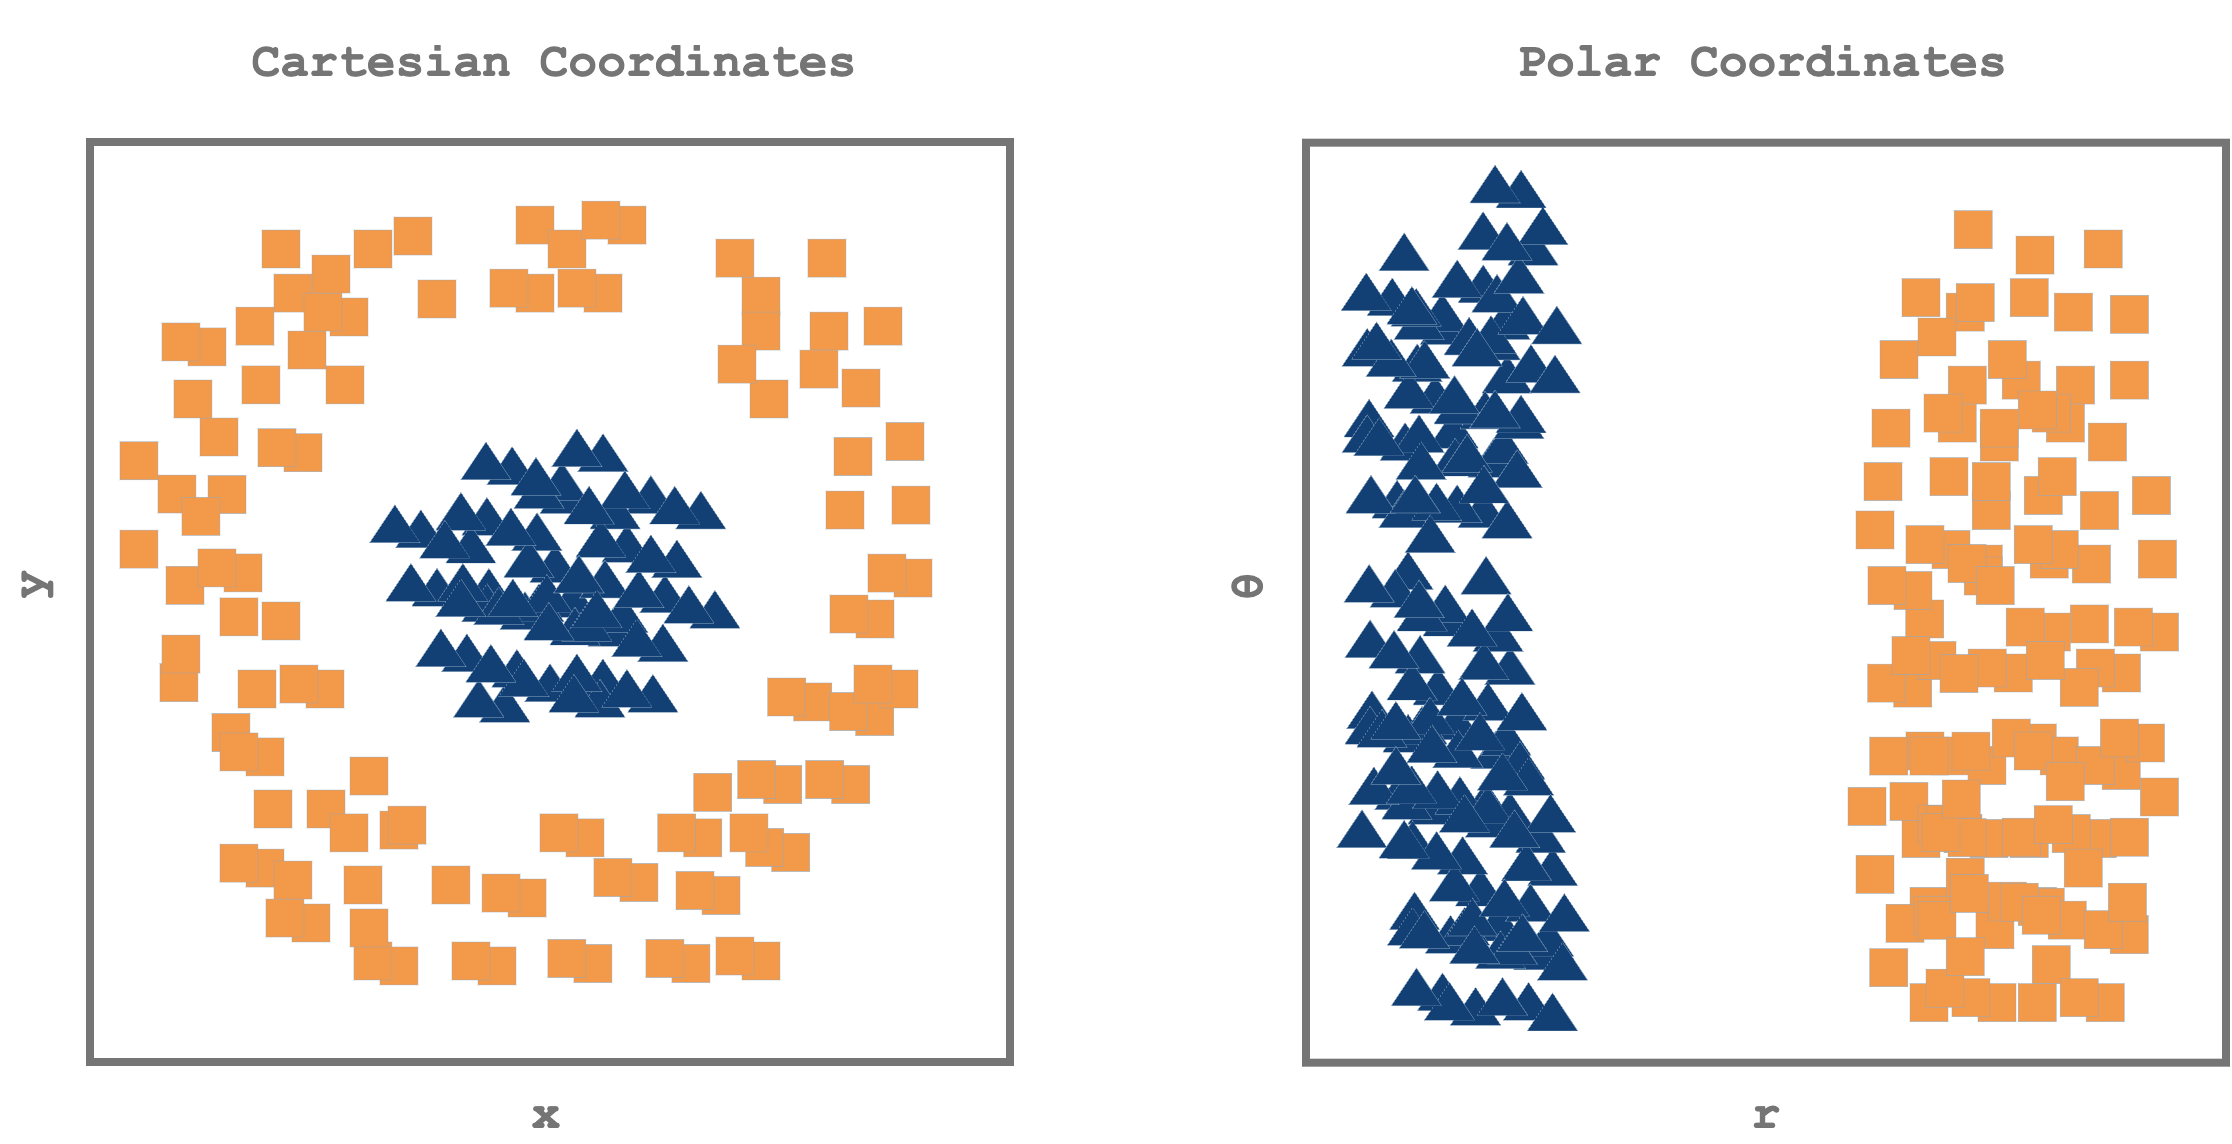
\includegraphics[width=0.8\textwidth]{Figures/representations.png}
    \caption{Illustration of representation learning: in Cartesian space the blue inner cluster and orange outer ring require a complex boundary, but in polar coordinates they separate linearly along the radial axis.}
    \label{fig:representations}
\end{figure}

The world's complexity could not be modeled linearly, often requiring non-linearity to capture complex relationships between concepts. For instance, separating foreground objects from camouflage backgrounds often requires a non‑linear transformation such as a colour‐opponent space (e.g.\ CIELAB \cite{CIELAB2018}), which renders the decision boundary almost linear.

A common task of a supervised learning\footnote{Self‑supervised and contrastive objectives have become the default pre‑training paradigm for large‑scale models, but supervised
examples remain essential for calibration and evaluation.} system is to predict an output $\hat{\bold{y}} \in \mathbb R^k$ from some input $\bold x \in \mathbb R^d$. That process can be called $f$ where $\hat{\bold{y}} = f(x)$. With the following simple equation,
\begin{equation}
    \hat{\bold{y}} = \sigma(W\bold x + \bold b),
    \label{eq:neuron}
\end{equation}
we can tweak the values of $W, b$ and $\sigma$ to produce accurate estimates of $\hat{y}$ if we have a valid training set to work with $\mathcal{D} = \{\bold x^{(i)}, \bold y^{(i)}\}^N_{i=1}$ where $\bold x^{(i)} \in \mathbb R^d$ and $\bold y^{(i)} \in \mathbb R^k$. $W$ is weight, $\bold b$ is bias and $\sigma$ is a non-linear activation function such as ReLU or sigmoid.

Stacking multiple units of \cref{eq:neuron} together into $L$ layers provides the depth necessary for more complicated representations to emerge.
\begin{equation}
    \bold a^{(\ell)} = \sigma(W^{(\ell)}\bold a^{(\ell -1)} + \bold b^{(\ell)}),\quad \ell = 1,\ldots ,L.
    \label{eq:layer}
\end{equation}

The final prediction can be computed by running a forward-pass from $\bold a^{(0)} = \bold x$ all the way through $L$ layers to $\hat{\bold y} = \bold a^{(L)}$. The first prediction will not be very good since the set of weights $W^{(\ell)} \in \mathbb R^{n_{\ell}\times n_{\ell - 1}}$ have not been updated to bring the predictions as close as possible to the original training set $\mathcal D$. This can be solved by minimizing the loss between $y_i$ and $\hat{y}_i$ with a loss function 
\begin{equation*}
    J(\theta) = \dfrac{1}{N} \sum_{i = 1}^{N} L(\bold{y}^{(i)},  \hat{\bold{y}}^{(i)}).
\end{equation*}
Typically this is performed by a gradient-based optimization, namely gradient-descent where there parameters are updated via $\theta \leftarrow \theta -\eta \nabla_{\theta}J(\theta)$ where $\theta \in \{W^{(\ell)}, b^{(\ell)}\}^L_{\ell=1}$ and $\eta$ configures the \textit{learning rate}.

Running this algorithm separately to improve the predictive $f$ capability is the machine learning; which becomes deep learning when $L > 2$.

The deeper the network the more complicated features it can learn. However the deeper it becomes the more parameters there are to train and the harder it is to \textit{understand} what is actually going on inside the black box $f$. 

Residual connections~\cite{RESNET2016} enable gradients to bypass
poorly conditioned layers, effectively learning a series of
incremental $\Delta f$ refinements rather than an entire mapping from
scratch.  Formally, a residual block learns
$\mathbf{y} = f(\mathbf{x}) + \mathbf{x}$, where
$f$ is a small stack of convolutions and
$\mathbf{x}$ is the identity shortcut.  This simple reformulation
mitigates vanishing gradients and allows networks hundreds of layers
deep to converge reliably.

\subsection{Convolutional Neural Networks} 

Building on \cref{eq:layer}, neural networks can learn to predict outputs from a primitive vector-based dataset $\mathcal D$, but a useful extension is to give a capable network the ability to see in the real world. 

Take an input (also called feature map) $X \in \mathbb R^{H\times W \times C}$ with $W, H$ and $C$ as the width, height and channel depth\footnote{An \ac{RGB} image has $C = 3$ for red, green and blue.} of the image. Passing even a small \ac{RGB} map $X\in \mathbb R^{100\times 100\times 3}$ through a fully connected layer would require 10,000 weights per neuron. This quickly becomes intractable for large enough feature maps so they must be compressed with minimal feature loss; a prime function of a \ac{CNN}.

The feature map is convolved with a kernel $K \in \mathbb R^{k_H\times k_W \times C \times C'}$, producing the $(i,j)$th compressed output as (where $i$ and $j$ correspond to individual pixels),
\begin{equation*}
    Y_{i,j,c}^{(\ell)} = (X * K)_{i,j,c} = 
\sum_{u=1}^{k_H}\sum_{v=1}^{k_W}\sum_{c=1}^{C}
X_{i+u-1,\,j+v-1,\,c}^{(\ell - 1)}\;K_{u,v,c',c}^{(\ell)}.
\end{equation*}

The final output of each layer with kernel  $K^{(\ell)}$ and bias $b^{(\ell)}$is,
\begin{equation*}
    A_{i,j,c}^{(\ell)} = \sigma\left(Y_{i,j,c}^{(\ell)} + b^{(\ell)}\right),
\end{equation*}
where $\sigma$ is a non-linearity. Stacking $A^{(\ell)}$  gives the next layer’s input of shape $(H^{(\ell+1)}, W^{(\ell+1)} , C^{(\ell+1)})$ which are depend on the padding $P$ and stride $S$ parameters,
\begin{equation*}
    H^{(\ell)} = \dfrac{H^{(\ell - 1)} - k_H +2P}{S} + 1, \quad
W^{(\ell)} = \dfrac{W^{(\ell - 1)} - k_w +2P}{S} + 1.
\end{equation*}

\paragraph{Pooling.} 

To reduce spatial size the input $X \in \mathbb R^{H\times W \times C_{\text{in}}}$ to something smaller, pixel regions are \textit{pooled} into smaller subregions and passed to the next layer (red layers in \cref{fig:conv_arch}). This is often taken over the max or average of a $p\times p$ patch,
\begin{equation*}
P_{i,j}^{(\ell)} = \max_{0\le u,v < p} A^{(\ell)}_{ip+u, jp+v},\quad \text{or}\quad P_{i,j}^{(\ell)} = \dfrac{1}{p^2}\sum_{0\le u,v < p} A^{(\ell)}_{ip+u, jp+v}.
\end{equation*}

\begin{figure}[ht]
    \centering
    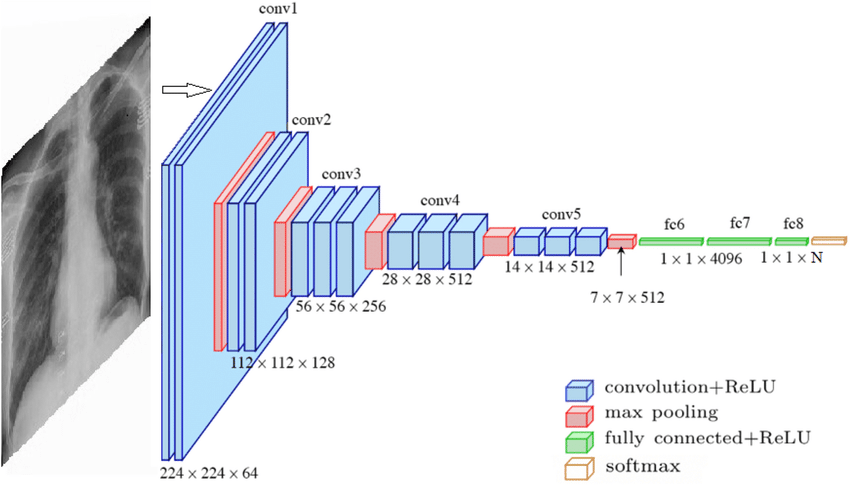
\includegraphics[width=0.7\textwidth]{Figures/conv-arch.png}
        \caption{Architecture of a deep convolutional network showing five convolutional blocks (blue: conv+ReLU, red: max-pooling) that transform a 224 × 224 × 3 input into a 7 × 7 × 512 feature map, followed by three fully connected layers (green: ReLU, orange: softmax) producing an $N$-way classification. Adapted from \textcite{CONVNETARCH2021}.}
    \label{fig:conv_arch}
\end{figure}

\paragraph{Fully Connected Layers.}

Convolutions and pooling are performed until the feature map has been reduced enough to a fully connected layer learn the features.

The final feature map is flattened into a vector $\bold h \in \mathbb R^D$ where $D$  is the product of the dimensions of the last pooling layer (green layers in \cref{fig:conv_arch}). Then final output is calculated using the softmax $\hat{\bold{y}} = \text{softmax}(W_{fc}\bold h+\bold b_{fc})$ which can be trained using  $\theta \leftarrow \theta - \eta \nabla_{\theta}L(\theta)$.

The \ac{CNN} was conceived by \textcite{CONV1980}, however it was \textcite{CONV1989} that introduced end-to-end supervised learning with trainable convolutional filters via backpropagation, formalized weight sharing, and demonstrated state-of-the-art handwritten digit recognition.

\paragraph{Vanishing Gradients.}

As networks grow deeper, gradients propagated through many layers tend to shrink toward zero, hindering effective weight updates in early layers. ResNets overcome this by adding identity skip connections,
\begin{equation*}
    A^{(\ell + 1)} = f(A^{(\ell)}) + A^{(\ell)},
\end{equation*}
that let gradients flow unimpeded through shortcut paths. This simple modification enables training of ultra-deep \ac{CNN} models without loss of signal \cite{RESNET2016}.

\paragraph{Compound Scaling.}

Scaling up \acp{CNN} to more layers can result in better accuracy as seen from ResNet-18 to ResNet-200 \cite{RESNET2016}. Although poorly understood, \ac{CNN} scaling can occur across three dimensions: width \cite{WIDERESNETS2016}, depth \cite{RESNET2016} or resolution scaling \cite{GPIPE2019}. \textcite{EFFICIENTNET2020} formulated a unified scaling framework by using single compound coefficient $\phi$ to scale depth, width and resolution from their baseline values $d^{(0)} = L, w^{(0)} = W$ and $r^{(0)}$. Each increment of $\phi$ roughly doubles compute by enforcing $ \alpha\,\beta^{2}\,\gamma^{2}\approx 2$, where $\alpha,\beta,\gamma>1$ are constants. The resulting dimensions are \begin{equation*}
(d,w,r) = \bigl(d^{(0)},\,w^{(0)},\,r^{(0)}\bigr) \odot \bigl(\alpha^{\phi},\,\beta^{\phi},\,\gamma^{\phi}\bigr).
\end{equation*}

\subsection{Autoencoders}

\acp{AE} are representation learning architectures that works in two parts: an encoder function $\bold h = f(\bold x)$ and decoder that produces reconstruction $\bold r = g(\bold h)$ with parameters $\{\theta_f, \theta_g\}$. It consists of a hidden layer $\bold h$ that describes the latent representation of the input to learn $g(f(\bold x)) \approx \bold x$ by, minimizing a loss 
\begin{equation*}
\min_{\theta_f, \theta_g} L(\bold x, g(f(\bold x)).
\end{equation*}

\acp{AE} come in many different forms, such as Sparse \acp{AE} $\min_{\theta_f, \theta_g} L(\bold x, g(f(\bold x)) + \Omega(\bold h)$ with a sparsity penalty $\Omega(\bold h)$ for classification \cite{SAE2024}, Denoising \acp{AE} $\min_{\theta_f, \theta_g} L(\bold x, g(f(\bold{\tilde{x}}))$ with $\bold{\tilde{x}}$ being a corrupted copy of $\bold x$ for filtering noise \cite{DAE2015} and others. \acp{VAE} are of particular interest where instead of propagating signals through a latent bottleneck $\bold h$ they impose a probabilistic prior on the latent space, 
\begin{equation*}
\min_{\theta_f,\theta_g}
\mathbb{E}_{f(\bold h\mid\bold x)}
[L(\bold x,\, g(\bold h))]
+ D_{\mathrm{KL}}\!\bigl(
  f(\bold h\mid\bold x)\,\|\,\mathcal{N}(0, I)
\bigr)
\end{equation*}
from $f(\bold h \mid\bold x) \sim \mathcal{N}(\mu, \sigma^2I)$, which yields continuous, disentangled representations that can be smoothly sampled to generate novel data like images \cite{VAE2020}\footnote{The \ac{KL} divergence measures how a distribution $q(\mathbf z)$ departs from a reference $p(\mathbf z)$: $D_{\mathrm{KL}}(q\,\|\,p)=\int q(\mathbf z)\log\bigl(\frac{q(\mathbf z)}{p(\mathbf z)}\bigr)\,d\mathbf z$. It is always non-negative, equals $0$ only when $q=p$, and is asymmetric \cite{KLDIV1951}.}.

\section{Transformers}

Sequence transduction modelling has been important for the fields of language translation and next token prediction,
\begin{align*}
    (x_1, x_2, \ldots, x_T) &\mapsto (\hat{y}_1, \hat{y}_2, \ldots, \hat{y}_{T'}) \\
    (x_1, x_2, \ldots, x_T) &\mapsto (\hat{y}_{T+1}),
\end{align*}
where $x_t \in \mathcal V_x, y_t \in \mathcal V_y$. \textcite{LSTM1997} introduced the \ac{LSTM} architecture for \acp{RNN}. \textcite{SEQ2SEQ2014} later used LSTMs for sequence-to-sequence learning. Calculating each hidden state $h_t = f(x_t, h_{t-1})$ requires the preceding state, which limits parallelism across time steps.

With the introduction of the transformer by \textcite{ATTENTION2023} paralleization was now possible with a new model architecture that calculated the self-attention between all tokens $(x_1, x_2, \ldots, x_T)$ in a sequence. Self-attention is computed by compiling three vectors: $\bold k = [k_1, k_2, \ldots, k_T]^T$ encoding the position of each token, $\bold q = [q_1, q_2, \ldots, q_T]^T$ the starting token, and $\bold v = [v_1, v_2, \ldots, v_T]^T$ a set of value vectors that store the information content of each token\footnote{In the literature $\bold k, \bold q$ and $\bold v$ are normally expressed as matrices $K, Q$ and $V$. Vectors were used here for exposition to highlight the per-token computation; in practice these are batched as matrices to enable efficient parallel processing.}. Mathematically, attention is the weighted sum\footnote{The sum of the product $\bold q_k \cdot \bold k_t$ should be evenly diffused to avoid softmax generating one-hot vectors, where very large values in the softmax can drown out the smaller values. We don’t want that. Hence it’s safer to scale the dot product i.e., $\bold q_k \cdot \bold k_t / \sqrt{d_k}$ where $d_k$ is the attention head size \cite{ATTENTION2023}.} from query vector $\bold q_k$,
\begin{equation*}
    \bold z _k = \text{Attention}(\bold q_k, \bold k, \bold v) = \sum^T_{t=0} \text{softmax}(\bold q_k \bold k_t^T) \bold v_t.
\end{equation*}

With the benefits of high parallezibility come from stacking multiple attention heads together into a multihead attention block,
\begin{align*}
    \text{MultiHeadAttention}(\bold q_k, \bold k, \bold v) &= \text{concat}(\text{head}_1(\bold q_k), \ldots,\text{head}_h(\bold q_k)) \\
    \text{where } \text{head}_i(\bold q_k) &= \text{Attention}(W_i^{Q} \bold q_k, W_i^{K} \bold k, W_i^{V} \bold v)W^O.
\end{align*}
Here the parameter matrices are $W_i^Q \in \mathbb{R}^{d_{\mathrm{model}}\times d_k}, W_i^K \in \mathbb{R}^{d_{\mathrm{model}}\times d_k}, W_i^V \in \mathbb{R}^{d_{\mathrm{model}}\times d_v}$ and $W^O \in \mathbb{R}^{h\,d_v\times d_{\mathrm{model}}}$.

This ability to capture long-range phenomena became noteworthy as language transduction models began to sound more human-like.

\begin{figure}[ht]
    \centering
    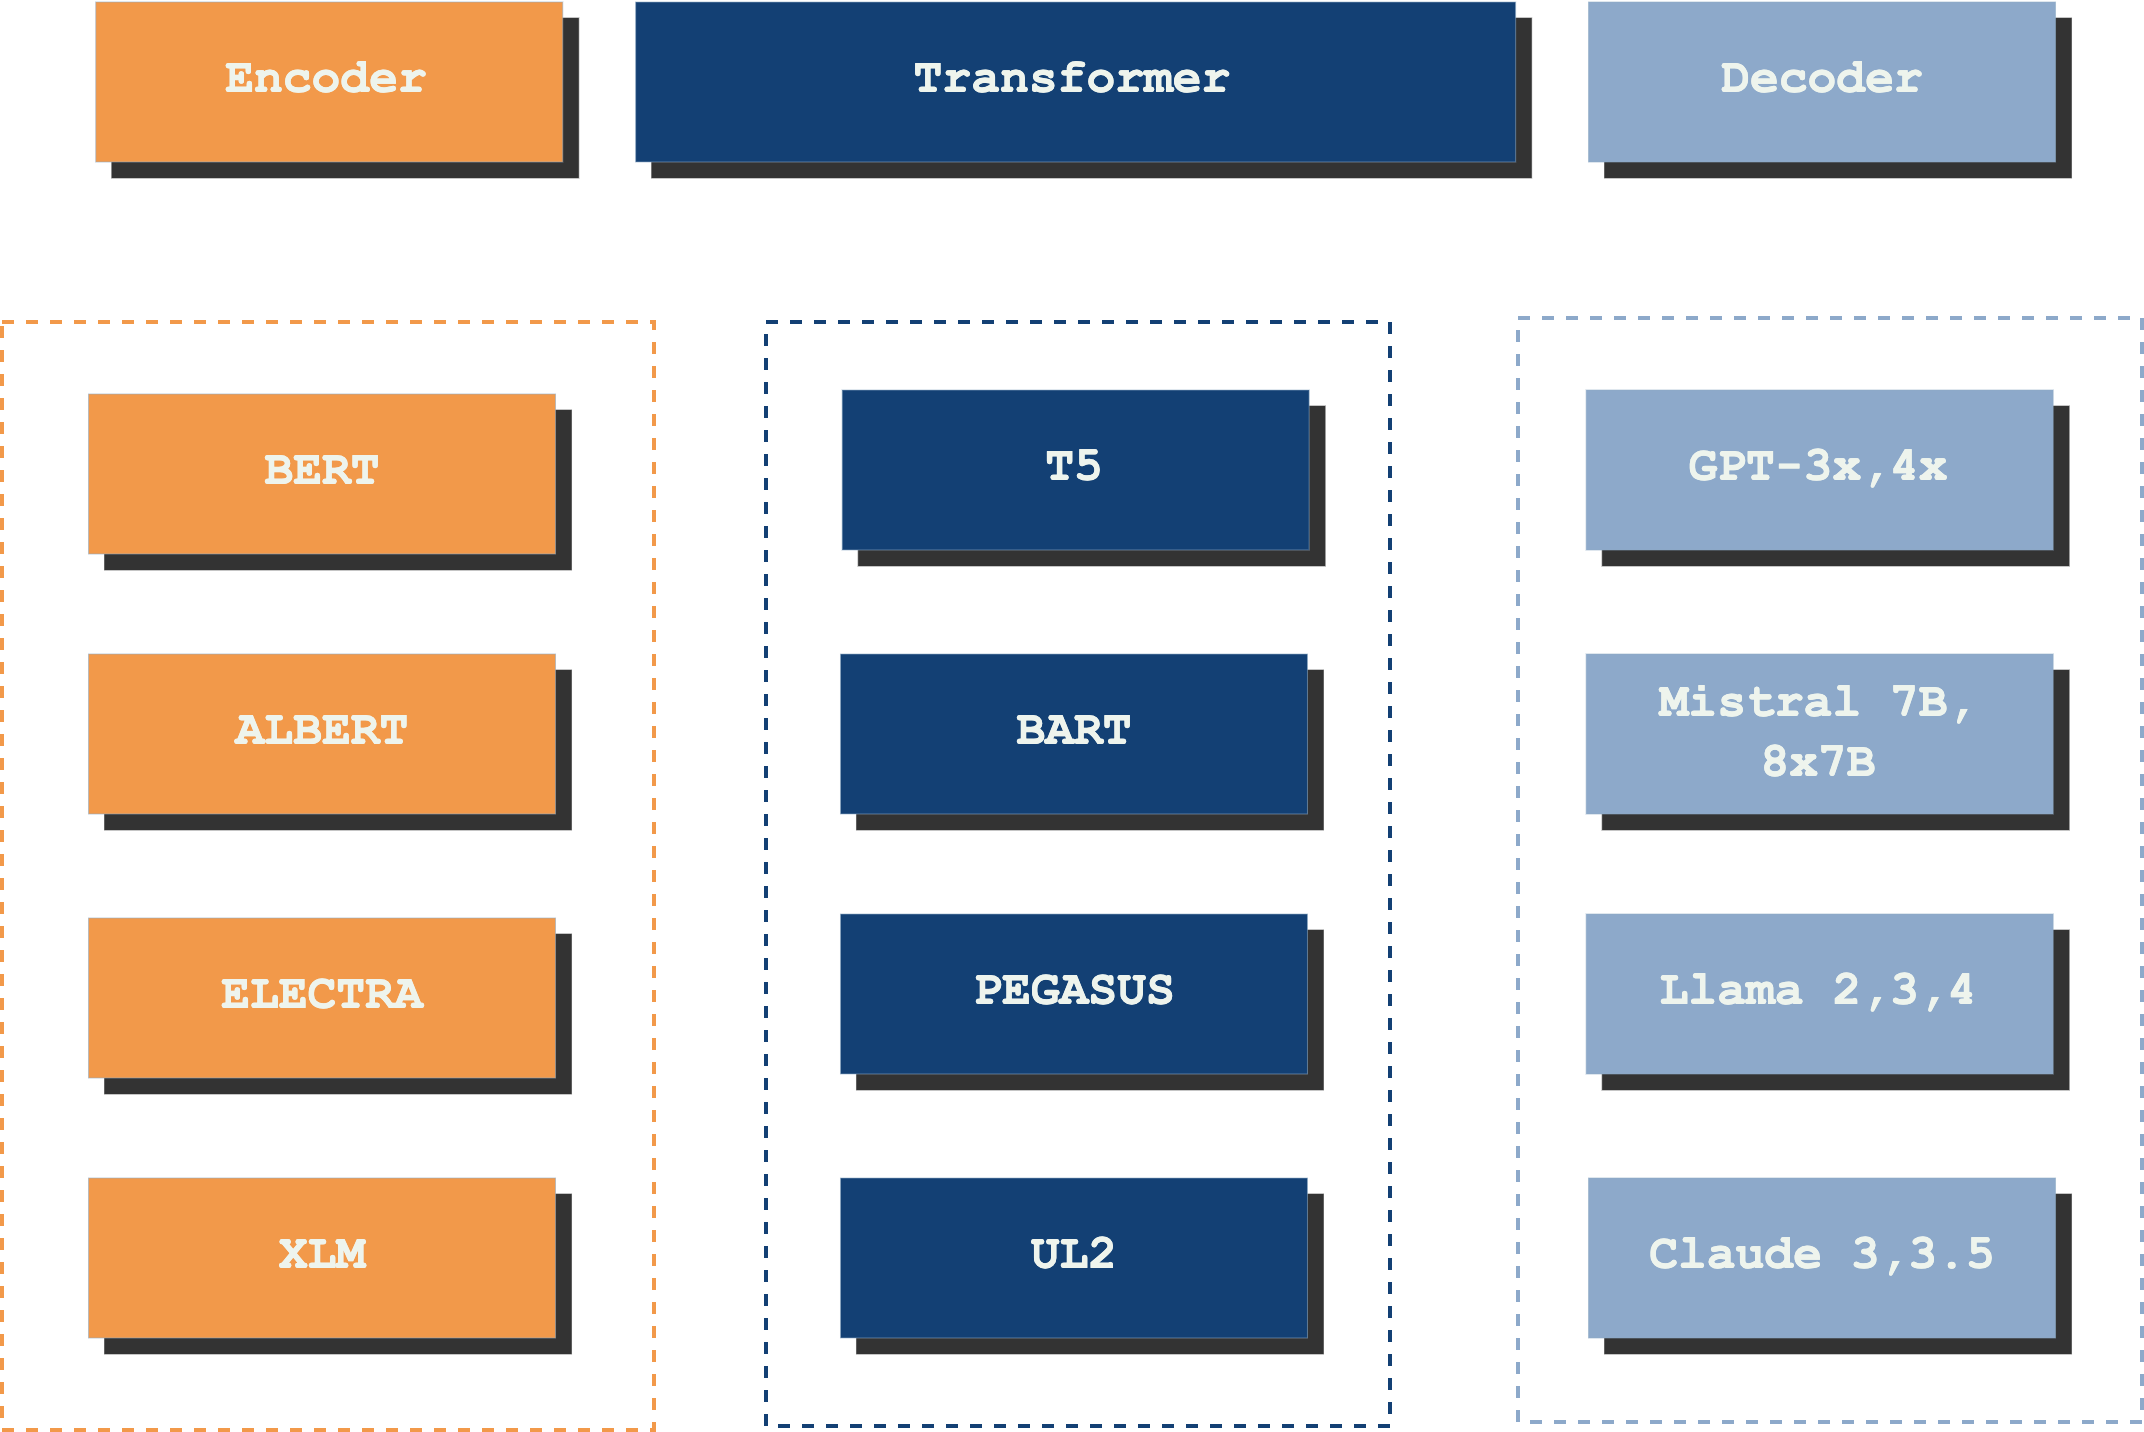
\includegraphics[width=0.8\textwidth]{Figures/transformers.png}
    \caption{Overview of transformer model families grouped by architecture. \textit{Left}: encoder only (BERT, ALBERT, ELECTRA, XLM). \textit{Middle}: encoder-decoder (T5, BART, PEGASUS, UL2). \textit{Right}: decoder only (GPT-3x/4x, Mistral 7B/8×7B, Llama 2/3/4, Claude 3/3.5).}
    \label{fig:transformers}
\end{figure}

\subsection{Large Language Models} 
\label{sec:llms}

Different types of transformers have emerged most notable decoder-only \cite{GPT32020}, encoder-only \cite{BERTGPT2023} and a encoder-decoder mix \cite{BART2019} as shown in \cref{fig:transformers}. Each has its advantages and disadvantages. Decoder-only transformers tend to perform better at open‑ended sequence generation, code synthesis and in‑context few‑shot prompting due to their autoregressive training. Encoder-only transformers perform better at discriminative tasks because of their \ac{MLM} bidirectional training.

Transformers, like any other neural network, can only take real numbers as inputs. Therefore translating language to numerical format, also known as tokenizing, can meaningfully dictate the capabilities of the language model. Nuemrous tokenizing schemes are employed today most notably WordPiece used by \ac{BERT} \cite{WORDPIECE2021} and \ac{BPE} used by \ac{GPT}-series \cite{BPE2024}. Formally, a tokenizer is a mapping $T:\Sigma^*\to V^*$ from an input string over alphabet $\Sigma$ to a sequence of tokens in vocabulary $V$ (with $|V|$ fixed). For any word $w\in\Sigma^*$ we write  
$T(w)=(s_1,s_2,\dots,s_k)$, where $s_i\in V$ and $w=s_1\circ s_2\circ\cdots\circ s_k$. Each token $s_i$ is then mapped to an integer ID via a lookup $f:V\to\{1,\dots,|V|\}$.

\paragraph{Byte-Pair Encoding.} Start with $V_0=\Sigma$ and counts $c_0(a,b)$ for every adjacent symbol pair $(a,b)$. At each merge step $t=1,\dots,N$, pick $(a^*,b^*)=\arg\max_{(a,b)}c_{t-1}(a,b)$,  
then define a new symbol $x=a^*b^*$ and update $V_t=V_{t-1}\cup\{x\}$ and counts by replacing all occurrences of $(a^*,b^*)$ with $x$. After $N=|V|-|\Sigma|$ merges, $V_N$ has the desired size. Tokenization greedily matches the longest symbol in $V_N$ at each step.

\paragraph{WordPiece.} Given corpus $C$, learn $V$ by maximizing the data likelihood under a subword model. One often maximizes  
\begin{equation*}
\max_V\prod_{w\in C}\sum_{(s_1,\dots,s_k)=w}\prod_{i=1}^k p(s_i\mid s_{<i}),
\end{equation*}
where $p(s_i\mid s_{<i})$ is estimated from subword counts. In practice a greedy heuristic adds the subword that most increases the log-likelihood until $|V|$ is reached.

% TODO
% \begin{importantbox}
% Backfil
% \end{importantbox}

\subsection{Vision Transformers} 

While the Transformer architecture \cite{ATTENTION2023} has become the de-facto standard for natural language tasks, it has proven to be effective at computer vision tasks when paired with an effect tokenizer and a high data regime (14M-300M images) \cite{16x162021}. Propagating an image $\bold x \in \mathbb R^{H\times W\times C}$ through a \ac{ViT}, requires it to be flattened into a linear sequence of patches $\bold x_p \in \mathbb R^{N\times (P^2C)}$ where $(P,P)$ is the resolution of each image patch and $N = HW/P^2$ is the resulting number of patchs. Patches can then be treated equal to word tokens in a natural language context allowing the model to be trained on tasks like image classification in a supervised fashion. \acp{ViT} have shown remarkable generalization when trained on a large corpus of images, even outperforming \acp{CNN} \cite{16x162021}.

\subsection{Vision Language Models} 
\label{sec:vlms}

\acp{VLM} extend the Transformer architecture to jointly model images and text. Modern \acp{VLM} fall into four broad families based on their pretraining objectives. Pioneering efforts such as Visual-\ac{BERT} and ViL\ac{BERT} embed image regions and words into a shared Transformer. They are trained on (a) masked token modelling to predict missing words or image regions, and (b) image–sentence matching to decide whether a caption describes an image \cite{VISUALBERT2019,VLBERT2019}.

\paragraph{Contrastive–based VLM.}
Models like \ac{CLIP} train separate image and text encoders on hundreds of millions of image–caption pairs using an InfoNCE loss. Matched pairs are pulled together in a shared embedding space while mismatched pairs are pushed apart. At inference, text prompts can retrieve semantically aligned images in zero-shot fashion (e.g.\ \ac{CLIP} with ResNet-101 attains 76.2\% zero-shot ImageNet accuracy) \cite{CLIP2021}.

SigLIP replaces \ac{CLIP}'s softmax-normalized contrastive loss with a pairwise sigmoid loss 
\begin{equation*}
    L_{\mathrm{sig}} = -\dfrac{1}{|\mathcal B|}\sum_{(i,j)\in\mathcal B}\bigl[y_{ij}\log\sigma(z_i\!\cdot\!z_j)+(1-y_{ij})\log(1-\sigma(z_i\!\cdot\!z_j))\bigr],
\end{equation*}
operating per image–text pair without global normalization and yielding improved zero-shot accuracy and batch-size scalability \cite{SIGLIP2023}.

\paragraph{Masking–based VLM.}
Masking approaches view \ac{VLM} pretraining as cross-modal denoising. FLAVA employs three Transformer encoders (image, text, multimodal) and combines unimodal/multimodal masked modelling with a contrastive loss, achieving state-of-the-art results on over 35 vision, language, and multimodal benchmarks after pretraining on 70 M image–text pairs \cite{FLAVA2022}. MaskVLM extends this by masking raw pixels and text tokens simultaneously, using each modality to help reconstruct the other \cite{MASKEDVLM2023}.

\paragraph{Generative–based VLM.}
Generative \acp{VLM} learn to produce text and/or images directly. CoCa adds a caption-generation loss atop contrastive training, enabling tasks like \ac{VQA} without extra fusion modules; it is pretrained on over 1 B images with alt-text annotations \cite{COCA2022}. Mixed-modal autoregressive models such as CM3Leon interleave image and text tokens in a single decoder, supporting both image-to-text and text-to-image generation with retrieval-augmented pretraining and supervised fine-tuning \cite{CM3LEON2023}.

\paragraph{VLM from Pretrained Backbones.}
To reduce compute and data demands, many \acp{VLM} map frozen pretrained encoders into each other's space. Frozen maps visual features (NF-ResNet-50) into a frozen 7B-parameter \ac{LLM}, fine-tuning only a lightweight projection head on Conceptual Captions for rapid zero-/few-shot multimodal capabilities \cite{FROZENLANGUAGE2021}. Mini\ac{GPT}-4 aligns BLIP-2's Q-Former+\ac{ViT} image embeddings to a Vicuna \ac{LLM} via a small projector trained on $\sim$5 M image–text pairs and an instruction-tuning step \cite{MINIGPT42023}.

\section{Reinforcement Learning}
\label{sec:rl_theory}

\begin{flushright}{\slshape    
    \textit{The most important thing for AI \\
    is to have systems that can \\
    learn from experience, like humans do.}} \\ \medskip
    --- \textsc{Yann LeCun} \cite{LECUNINTERVIEW2018}
\end{flushright}

\bigskip

\ac{RL} is a reward-based paradigm in which an agent improves its behavior through trial and error. Unlike supervised learning, which relies on labeled input–output pairs to minimize a predefined loss, and unsupervised learning, which uncovers structure without external feedback, \ac{RL} uses scalar rewards to guide policy improvement over time.

\subsection{Formal Framework}

An \ac{RL} problem is modeled as a \ac{MDP} defined by a 5-tuple $(\mathcal{S}, \mathcal{A}, P, r, \gamma)$. The transition function is defined as $P: S\times A \rightarrow S$ and the reward function is $r: S\times A \rightarrow \mathbb R$. In general, for solving any agent-world \ac{RL} task:
\begin{enumerate}
    \item At each time $t$ the agents observe the current state $s_t \in \mathcal{S}$
    \item Selects the appropriate action $a_t \in \mathcal{A}$ to perform
    \item Environment returns a reward $r_t=  r(s_t, a_t)$
    \item Agent transitions to state $s_{t+1} = P(s_t, a_t)$
\end{enumerate}

The goal should be to follow (and create) a policy $\pi: S \rightarrow A$ that maximizes the accumulated reward over time $V^\pi(s_t)$. That policy $\pi(a|s)$ maps states to action probabilities with the return from time $t$ as
\begin{equation*} 
    G_t = \sum_{k=0}^\infty \gamma^k r_{t+k+1},
\end{equation*}
with $\gamma \in [0,1)$ as the discount factor applied to each successive reward $r_t$ determining whether the agent is myopic $(\gamma =0)$ and foresighted $(\gamma = 1)$.

The value $v$ of a state $s$ under a policy $\pi$ is expressed as $V_\pi(s_t)$ or $V^\pi(s_t)$ depending on the textbook,
\begin{equation*} 
    V^\pi(s) = \mathbb{E}_\pi\bigl[G_t \mid s_t = s\bigr],
\end{equation*}

and the action–value function is
\begin{equation*} 
    Q^\pi(s,a) = \mathbb{E}_\pi\bigl[G_t \mid s_t = s,\;a_t = a\bigr].
\end{equation*}

The optimal policy $\pi^*$ then satisfies
\begin{equation*} 
\pi^*(s) = \argmax_a Q^\pi(s,a).
\end{equation*}

The search for $a$ is the ultimate goal of any \ac{RL} agent. There are two predominant methods: (1) if we know $Q(s,a)$ then solve for $a = \argmax_a Q(s,a)$, referred to as value-based methods and (2) first find $\pi(s)$ to then sample $a \sim \pi(s)$, referred to as policy-based methods. These will be the focus of the remainder of \S\ref{sec:rl_theory}.

\subsection{Value-Based Methods}

\paragraph{TD Learning.}

\ac{TD} agents learn from experience over time (i.e., temporally). Modeling their impact on an environment as a function of the current state and action taken can provide enough stimulus to inform successive decisions, 
$$
V(s_t) \leftarrow V(s_t)+\underbrace{\alpha}_{\text{learning rate}}\underbrace{\left[\underbrace{r_{t+1}}_{\text{reward}} + \underbrace{\gamma V(s_{t+1})}_{\text{discounted value of next state}} - V(s_t)\right]}_{\text{temporal difference}}.
$$
An action $a_t$ that is taken in state $s_t$ at time step $t$ in accordance with policy $\pi$ is denoted as $Q_\pi(s_t,a_t)$ which is the action-value function. With the optimal policy $\pi^*$ one can arrive at the optimal action-value function,
$$
Q^*(s_t,a_t) = \max_\pi Q^\pi(s_t, a_t).
$$

\paragraph{Q-Learning.}

The agent maintains a table of action-value estimates, $Q(s,a)$, which it updates at each time step using the Bellman equation. This table records expected returns for every state–action pair and serves as a dynamic reference for decision making. Because updates are based on the highest-valued actions rather than the behavior policy $\pi$, this approach is classified as off-policy control \cite{QLEARNMULTIAGENT2015}.

\begin{algorithm}
\caption{Q‑Learning with Flexible Action‑Selection}
\label{alg:qlearning_flex}
\begin{algorithmic}[1]
  \Require learning rate $\alpha$, discount $\gamma$, episodes $M$
  \Require decay factors $\lambda$ (for $\varepsilon$) and $\kappa$ (for $\tau$)
  \Require \texttt{policyType} $\in\{\text{greedy},\ \varepsilon\text{-greedy},\ \text{softmax}\}$
  \State Initialise $Q(s,a)\gets 0$ for all $s\in\mathcal{S}$, $a\in\mathcal{A}$
  \For{episode $=1$ to $M$}
    \State $S\gets$ initial state
    \For{$t=0$ \textbf{until} $S$ is terminal}
      \If{\texttt{policyType} $==$ \texttt{greedy}}
        \State $A\gets\arg\max_{a} Q(S,a)$
      \ElsIf{\texttt{policyType} $==$ \texttt{$\varepsilon$-greedy}}
        \State $\varepsilon \gets e^{-\lambda t}$
        \State Choose $A$ randomly with prob.\ $\varepsilon$ else $A\gets\arg\max_{a} Q(S,a)$
      \Else \Comment{softmax}
        \State $\tau \gets e^{-\kappa t}$
        \State Sample $A$ from $\displaystyle P(a)=\frac{\exp \bigl(Q(S,a)/\tau\bigr)}{\sum_{i}\exp \bigl(Q(S,i)/\tau\bigr)}$
      \EndIf
      \State Take $A$, observe $R$ and next state $S'$
      \State $Q(S,A)\gets Q(S,A)+\alpha\bigl[R+\gamma\max_{a}Q(S',a)-Q(S,A)\bigr]$
      \State $S\gets S'$
    \EndFor
  \EndFor
\end{algorithmic}
\end{algorithm}

In greedy action selection shown in \cref{alg:qlearning_flex}, the agent always chooses the highest-valued action, maximizing immediate reward but risking premature convergence to suboptimal behaviors. The $\varepsilon$-greedy policy mitigates this by selecting a random action with probability $\varepsilon$ (which decays over time) and otherwise exploiting the best known action; this ensures initial exploration of the state–action space while gradually shifting toward exploitation. The softmax policy offers a smoother trade-off by sampling actions according to a Boltzmann distribution over Q-values, controlled by a ``temperature'' $\tau$: high $\tau$ yields near-uniform exploration, low $\tau$ concentrates probability on the best actions. Thus, greedy maximizes exploitation, $\varepsilon$-greedy balances exploration and exploitation via occasional random moves, and softmax provides graded exploration proportional to relative action values.

\paragraph{SARSA.}

In \ac{SARSA} an update $(S_t, A_t, R_{t + 1}, S_{t + 1}, A_{t + 1})$ depends on the action that the behaviour policy $\pi$ actually executes, so the algorithm's evaluation and control are fully coupled. With a purely greedy policy the agent always selects $A_{t+1}=\arg\max_a Q(S_{t+1},a)$; \ac{SARSA} then improves rapidly but can still inherit any risk that stems from stochastic transitions. Under a decaying $\varepsilon$-greedy policy the same update incorporates exploratory actions with probability $\varepsilon$, producing more conservative value estimates that often yield safer paths than those found by off‑policy Q‑learning. If $\pi$ is a softmax policy, the contribution of $Q(S_{t+1},A_{t+1})$ is weighted by a Boltzmann distribution whose temperature $\tau$ gradually cools, allowing the algorithm to hedge among near‑optimal actions before committing. Thus greedy \ac{SARSA} maximises exploitation, $\varepsilon$-greedy \ac{SARSA} balances exploration and exploitation explicitly, and softmax \ac{SARSA} provides a graded, uncertainty‑aware compromise; each choice trading convergence speed against robustness to sub‑optimal early estimates.

\subsection{Policy-Based Methods}



\paragraph{Policy Gradient.}

The goal of policy learning is to directly optimize $\pi_{\theta}(a|s) \sim \mathcal N(\mu, \sigma)$ such that $\theta \in \mathbb R^d$ to sample the next best action $a \sim \pi(s)$. This can be achieved my maximizing the expected (discounted) return,
\begin{equation} 
J(\theta)=\mathbb{E}_{\pi_{\theta}}\Bigl[\sum_{t=0}^T\gamma^t r_t\Bigr]. 
\label{eq:rl_expected_return}
\end{equation}
Computing the gradient of \cref{eq:rl_expected_return}, $\nabla_{\theta}J(\theta)$ using the policy gradient theorem yields,
$$
\nabla_{\theta}J(\theta) = \mathbb E_{\pi_{\theta}}\left[\sum_{t=0}^T \nabla_{\theta}\log \pi_{\theta}(a_t|s_t)Q^{\pi}(s_t,a_t)\right].
$$
Gradient ascent can be used to the optimal $\pi^*(s)$.

\paragraph{Variance Reduction.}
The above gradient calculation incorporates high amounts of variance, so modifications can be made to ensure training is more stable with the choice of $\Psi_t$ in,
$$
\nabla_{\theta}J(\theta) = \mathbb E_{\pi_{\theta}}\left[\sum_{t=0}^T \Psi_t \nabla_{\theta}\log \pi_{\theta}(a_t|s_t)\right],
$$
from the following \cite{ADVEST2018},
\begin{enumerate}
\item $\sum_{t=0}^\infty r_{t}$ total reward for the trajectory
\item $\sum_{t'=t}^\infty r_{t'}$ reward following action $a_t$
\item $\sum_{t'=t}^\infty r_{t'} - b(s_t)$ baselined version of (2)
\item $Q^{\pi}(s_t,a_t) = \mathbb E_{\substack{s_{t+1}:\infty,\\ a_{t+1}:\infty}}\left[
\sum_{l=0}^{\infty}r_{t+l}
\right]$ state-action value function
\item $A^\pi(s_t,a_t) = Q^{\pi}(s_t,a_t) - V^{\pi}(s_t)$  advantage function
\item $r_t + V^\pi(s_{t+1}) - V^\pi(s_t)$ \ac{TD} residual where $V^{\pi}(s_t) = \mathbb E_{\substack{s_{t+1}:\infty,\\ a_{t}:\infty}}\left[
\sum_{l=0}^{\infty}r_{t+l}
\right]$
\end{enumerate}

Once a concrete value for $\nabla_{\theta}J(\theta)$ is selected, gradient updates are straightforward,

$$
\theta \leftarrow \theta + \alpha \nabla_{\theta}J(\theta).
$$

\subsection{Hybrid Methods}

\paragraph{Actor-Critic}
\begin{flushright}{\slshape    
    \textit{Give me six hours to chop down a tree and\\
    I will spend the first four sharpening the axe.}} \\ \medskip
    --- \textsc{Abraham Lincoln}
\end{flushright}

\bigskip

Actor–critic methods integrate policy‑gradient (actor) and value‑function (critic) ideas in a single on‑policy loop. The actor, parameterized by $\theta$, selects actions and is updated with the critic’s feedback, while the critic, parameterized by $w$, learns a low‑variance estimate of either $V_w(s)$ or $Q_w(s,a)$ as described in detail in \cref{alg:actor_critic}. The \ac{TD} error $\delta_t$ couples the two, yielding faster, more stable convergence than pure policy‑gradient and better asymptotic performance than value‑only control.

\begin{algorithm}
\caption{On‑Policy Actor–Critic (Q‑form)}
\label{alg:actor_critic}
\begin{algorithmic}[1]
  \State Initialise $s,\;\theta,\;w$ randomly
  \State Sample $a \sim \pi_{\theta}(a\mid s)$
  \For{$t = 1$ to $T$}
      \State Sample reward $r_t \sim R(s,a)$ and next state $s' \sim P(s'\mid s,a)$
      \State Sample next action $a' \sim \pi_{\theta}(a'\mid s')$ \Comment{on‑policy}
      \State $\displaystyle\theta \leftarrow \theta + \alpha_{\theta}\,Q_w(s,a)\,\nabla_{\theta}\log\pi_{\theta}(a\mid s)$
      \State $\displaystyle\delta_t \gets r_t + \gamma\,Q_w(s',a') - Q_w(s,a)$
      \State $\displaystyle w \leftarrow w + \alpha_{w}\,\delta_t\,\nabla_{w} Q_w(s,a)$
      \State $s \leftarrow s'\,,\quad a \leftarrow a'$
  \EndFor
\end{algorithmic}
\end{algorithm}

\paragraph{Trust Region Optimization.}

A policy parameter update step, $\theta \leftarrow \theta + \alpha \eta$ creates a new policy from the old counterpart $\pi_{\theta_{\text{old}}}$. If the gradient update is stable i.e., $\eta$  does not blow up then the ratio of the two should be relatively low.

\ac{TRPO} enforces this using a \ac{KL} divergence constraint,
$$
\mathbb E [{\text{KL}}(\pi_{\theta_{\text{old}}}(.\,| s) \| \pi_{\theta}(.\,| s))] \le \delta, \quad D_{\text{KL}}(p \|q) = \int _x p(x) \log \dfrac{p(x)}{q(x)} \, dx.
$$
where $\delta \in \mathbb R$ is a hyperparameter \cite{TRPO2017}.

\paragraph{Proximal Policy Optimization.}

\ac{PPO} replaces \ac{TRPO}'s second‑order trust‑region constraint with a first‑order penalty that is easier to compute yet preserves stability \cite{PPO2017}.  Given an old policy $\pi_{\theta_{\text{old}}}$ and an updated policy $\pi_\theta$, define the probability ratio
$$
r(\theta)=\frac{\pi_\theta(a\mid s)}{\pi_{\theta_{\text{old}}}(a\mid s)}.
$$
If $\hat{A}_{\theta_{\text{old}}}(s,a)$ is a high‑quality advantage estimate, vanilla policy‑gradient would maximize
$$
J^{\text{TRPO}}(\theta)=\mathbb{E}_{\pi_{\theta_{\text{old}}}}\bigl[r(\theta)\,\hat{A}_{\theta_{\text{old}}}(s,a)\bigr].
$$
Large deviations of $r(\theta)$ from unity, however, can cause destructive updates.  \ac{PPO} therefore clips the ratio to the interval $[1-\epsilon,\,1+\epsilon]$ with a hyperparameter $\epsilon$, yielding the clipped surrogate
$$
J^{\mathrm{CLIP}}(\theta)=\mathbb{E}_t\!\left[\min\!\Bigl(r_t(\theta)\,\hat{A}_t,\;
\operatorname{clip}\bigl(r_t(\theta),1-\epsilon,1+\epsilon\bigr)\hat{A}_t\Bigr)\right].
$$
If the sign of $\hat{A}_t$ is positive, the clip caps overly aggressive improvements; if negative, it limits harmful drops in probability.  The objective thus enforces a soft trust region without computing \ac{KL} divergences, Hessian–vector products, or line searches.

For practical training the surrogate is combined with a squared‑error value loss and an entropy bonus that encourages exploration:
$$
J^{\mathrm{CLIP}'}(\theta)=
J^{\mathrm{CLIP}}(\theta)
-c_1\bigl(V_\theta(s)-V_{\text{target}}\bigr)^{2}
+c_2\,H\!\bigl(s,\pi_\theta(\cdot)\bigr),
$$
where $V_\theta$ is the critic, $H$ is policy entropy, and $c_1, c_2$ balance the three terms.  Optimization proceeds with first‑order stochastic gradient ascent using multiple epochs and minibatches drawn from the same trajectory batch.  Empirically, \ac{PPO} matches or exceeds \ac{TRPO}'s performance while being simpler to implement and significantly faster per update.

\subsection{Methodological Considerations}

Value‑based algorithms learn quickly with low variance because each transition updates many state–action estimates, yet they rely on an explicit maximisation step that becomes expensive or brittle in large or continuous action spaces. Policy‑based algorithms sidestep this maximisation and naturally support continuous or stochastic behaviours, but their gradient estimates contain high variance and therefore consume far more samples. Hybrid actor–critic schemes exploit the strengths of each approach: a critic supplies low‑variance value targets to guide the actor, while the actor eliminates the costly arg‑max. This compromise tends to deliver steadier learning and better scalability for real‑world robotics and control tasks, where action spaces are high‑dimensional and data collection is costly.

\section{Embodied Intelligence and AGI}

% \epigraph{``It is comparatively easy to make computers exhibit adult level performance on intelligence tests or playing checkers, and difficult or impossible to give them the skills of a one-year-old when it comes to perception and mobility.''}{Hans Moravec \cite{MORAVEC1988}}

\begin{flushright}{\slshape    
    \textit{It is comparatively easy to make computers exhibit \\
    adult level performance on intelligence tests or playing \\
    checkers, and difficult or impossible to give them the \\
    skills of a one year old when it comes to perception \\
    and mobility.}} \\ \medskip
    --- \textsc{Hans Moravec} \cite{MORAVEC1988}
\end{flushright}

Modern consensus holds that intelligence emerges from the closed action loop between an agent and its environment. Embodiment theory therefore argues that a robot must \emph{experience} the world through its own sensorimotor contingencies to acquire transferable concepts. \acp{VLA} offer rich perceptual priors, while \ac{RL} supplies the machinery for continual interaction‑driven learning; together they form a plausible path toward embodied \ac{AGI}.  Throughout the review we emphasize how this triad-vision, language and action-grounds abstract reasoning in physical competence, a prerequisite for safe autonomous robots operating in open worlds.

% Notes to add: Infuse data (and citation) from EGI aka AI 2027 and construct thesis around we need a path to EGI to have useful domestic robots.

\newpage
\chapter{Robotic Foundation Models}
\label{sec:rfms}

The term ``foundation model'' in \ac{AI} refers to large models (often trained on vast data from the internet) that provide a general base which can be adapted to many downstream tasks. In robotics, foundation models are emerging as a way to achieve generalist behavior across many tasks and environments, leveraging multimodal understanding. Two lines of work converged here: (a) multi-task learning in robotics, where a single network is trained to perform many different tasks (across possibly different embodiments), and (b) vision-language models that exhibit general-purpose understanding and reasoning. The combination leads to \ac{VLA} models; policies that ingest visual observations and language instructions, and output robotic actions.

\section{Transformer Foundation Models}

The early work on Gato demonstrated transformer-based generalism across multiple domains. Gato was trained on 604 distinct tasks spanning vision, language, and control, from captioning images to playing Atari games and controlling a real robot arm \cite{GATO2022}. With a single set of weights, Gato could accomplish diverse tasks, including robotic manipulations. For instance, on a real-robot block stacking benchmark, Gato could stack objects of novel shapes with success rates comparable to a specialized imitation-learning policy \cite{GATO2022}. This suggests that large transformers can learn a multi-task prior that generalizes to some new variations. However, Gato’s performance also underscored limitations: while it mastered many training tasks, solving an entirely new task outside its training distribution still required fine-tuning or additional data \cite{GATO2022}.

Transformers have also been applied to narrow domains such as planning. SayCan used an \ac{LLM} to interpret high-level instructions and suggest possible robot actions, which were then executed by low-level policies \cite{SAYCAN2022}. SayCan demonstrated robots responding to commands like ``bring me a water bottle'' by decomposing them, but the approach was modular (LLM + separate learned skills) rather than end-to-end.

PaLM-E (Embodied PaLM) is another broad model, embedding sensor observations into a language model context, enabling a form of \ac{LLM}-planning for robotics (e.g. reasoning about visual inputs and issuing actions) \cite{PALM2023}. These broader models extend the concept of a ``robotic foundation model'' beyond just direct visuomotor policies, towards multimodal reasoning agents. The theoretical promise is an embodied general intelligence that flexibly applies knowledge to new scenarios, yet practically they reveal how far current models must go to truly generalize in the real world.

A landmark was Robotics Transformer 1 (RT-1), which collected 130,000 demonstrations across 700+ household tasks for a mobile manipulator and trained a Transformer policy that takes image and textual goal description, and outputs motor commands \cite{RT12022}. RT-1 achieved robust multi-task performance (e.g. picking up arbitrary objects specified by language) within its training distribution. 

\section{VLA Foundation Models}

\subsection{Architecture}

Recent breakthroughs introduce \ac{VLA} models as large-scale ``foundation'' policies that integrate vision and language understanding to directly generate low-level robot actions. By leveraging pre-trained vision-language knowledge from the web and massive multi-task training, these models aim to provide generalist skills out-of-the-box and zero-shot adaptation to new instructions, drastically reducing the need for task-specific programming or extensive new demonstrations.

\acp{VLA} extend the capabilities of \acp{VLM} and \acp{LLM} by incorporating an action-generation component, as illustrated in \cref{fig:vla-arch}. These models unify perception and instruction understanding into an end-to-end system that produces control outputs, enabling robots to act on internet-scale knowledge with minimal task-specific engineering.

\begin{figure}[ht]
    \centering
    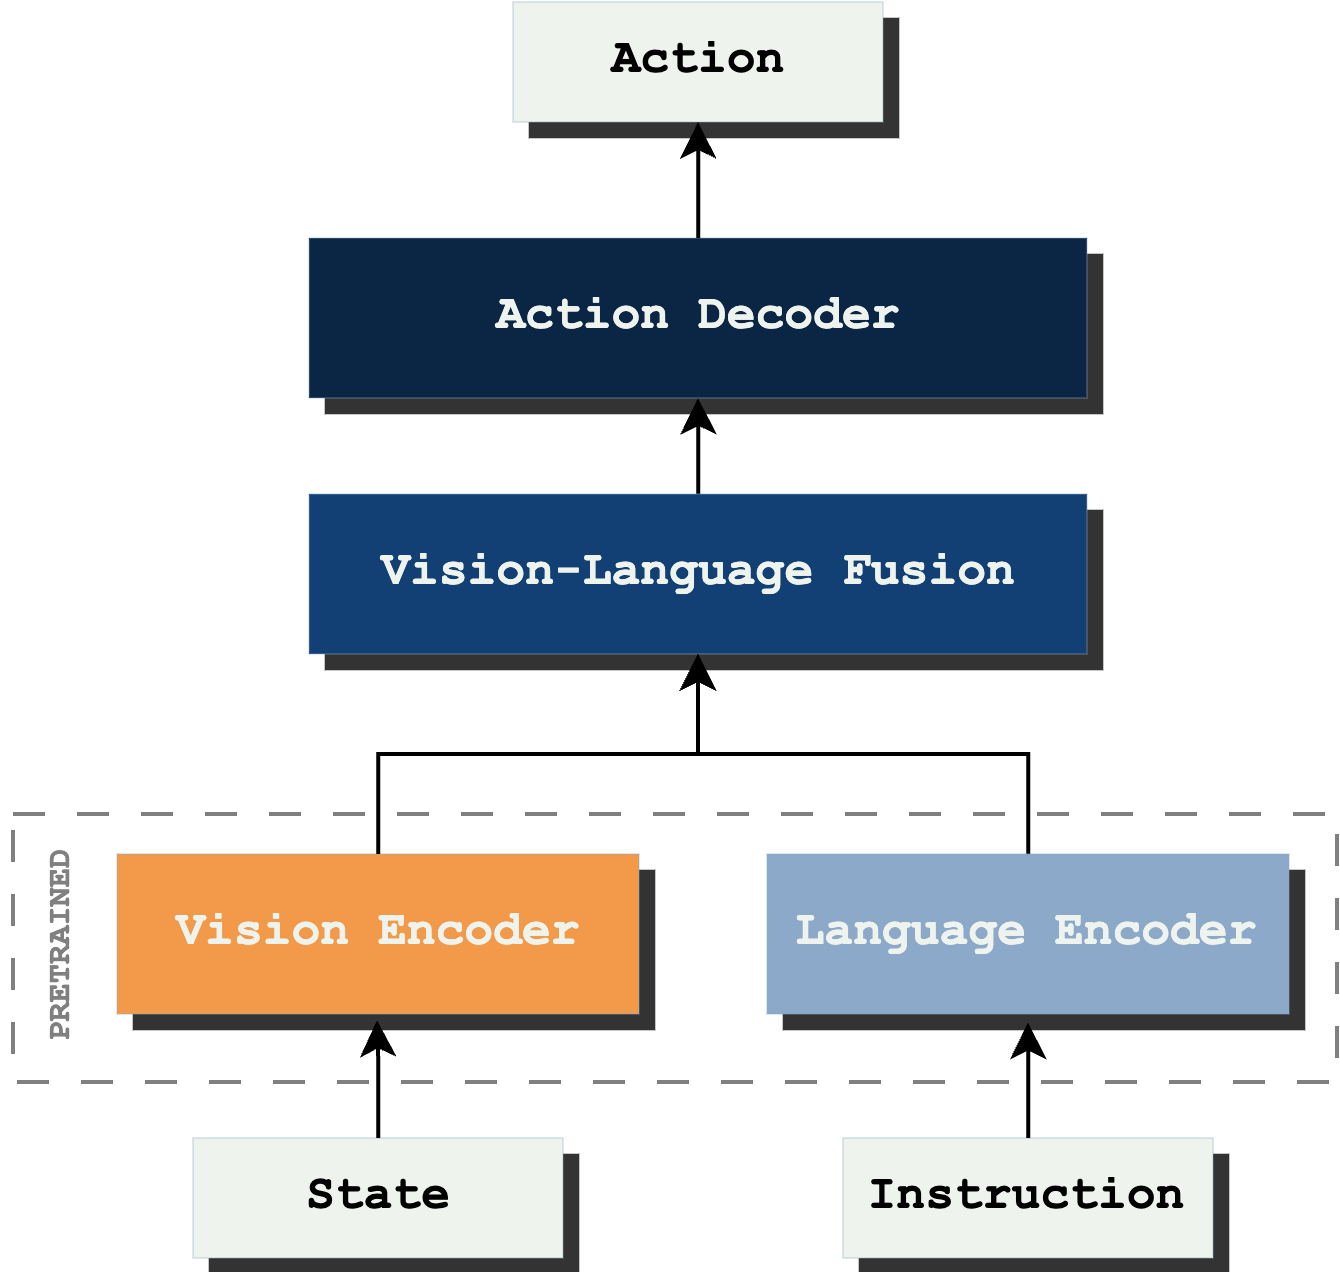
\includegraphics[width=0.5\textwidth]{Figures/vla-arch.png}
    \caption{\ac{VLA} architecture. A pretrained vision encoder ingests the robot's state and a pretrained language encoder processes the instruction. Their outputs feed into a shared action decoder, which generates the final action command.}
    \label{fig:vla-arch}
\end{figure}

The current landscape of \ac{VLA} models employ a variety of visual encoder backbones, namely \acp{CNN} \cite{MCIL2021,HULC2022,HULC++2022,PERACT2023, MTACT2024,OCTO2024}, ResNets \cite{CLIPORT2022,ACT3D2023,RVT2023,RVT22024,BCZ2022,ACT2023,DIFFPOLICY2023,SUDD2023, INTLANG2023, GATO2022}, EfficientNets \cite{QTRANSFORMER2023,RTTRAJ2023, RT12022}, \acp{ViT} \cite{LANGCOSTS2022,ROBOPOINT2024,VIMA2023,FLAMINGO2024,VOXPOSER2023,RTH2024,RTX2024, PI02024, OPENVLA2024, GR00T2025}, and hybrid \ac{ViT}-ResNets \cite{MDT2024} to compress visual input into a feature $v \in \mathbb R^{d_v}$. Each leverages different inductive biases, offering a spectrum of trade-offs between representational richness and computational efficiency \cite{VLASURVEY2025}. \acp{ViT} have exhibited superior accuracy relative to \ac{CNN} architectures under data-rich regimes, while requiring substantially less compute to train \cite{16x162021}. 

Visual encoding is only one half of the encoding process. Language encoders often use either a \ac{GPT} decoder-only \cite{CLIPORT2022, LANGCOSTS2022, INTLANG2023, PERACT2023, ACT3D2023, RVT2023, RVT22024, ROBOPOINT2024, FLAMINGO2024, VOXPOSER2023, SUDD2023, MDT2024}, \ac{BERT} encoder-only \cite{HULC2022, HULC++2022} or encoder-decoder \cite{BCZ2022, RT12022, QTRANSFORMER2023, VIMA2023, OCTO2024, RT22023, RTH2024, RTX2024} architecture to compress language input into a feature $\ell \in \mathbb R^{d_{\ell}}$. Relative performance of \ac{GPT} and \ac{BERT}-style models varies across different tasks e.g., paraphrasing vs predicting \cite{BERTGPT2023}.

The vision language fusion module then computes a joint representation $f = \psi(v, \ell) \in \mathbb R^{d_f}$ via cross-attention or \ac{FiLM} \cite{FiLM2017} for an action-decoder to produce a distribution over actions by 
\begin{equation*}
    \pi(a|f) = \text{softmax}\left(Wf+b\right),
\end{equation*}
where $\mathcal{A} = \{a_1, a_2, \ldots, a_{n}\}$, $W\in \mathbb R^{|\mathcal{A}|\times d_f}$ and $b \in \mathbb{R}^{|\mathcal{A}|}$. The final action output might include 6-\ac{DoF} \ac{SE3} end-effector velocities $a = [\dot{x}, \dot{y}, \dot{z}, \dot{\phi}, \dot{\theta}, \dot{\psi}]$, a binary gripper command \cite{RT22023} and the mean and covariance of the uncertainty in the velocities $a\sim \mathcal{N}(\mu_f, \Sigma_f)$ \cite{FLAMINGO2024, VOXPOSER2023}.

\subsection{Comparative Analysis}

Building on the architectural overview above, we now compare five representative \ac{VLA} systems across shared design axes and real-world benchmarks. RT-2 integrates a \ac{ViT} visual encoder with a \ac{GPT}-style decoder and softmax action head, yielding 62\% zero-shot success on novel-object pick-and-place tasks, an improvement from its predecessor RT-1 \cite{RT12022} driven by web-scale vision pretraining \cite{RT22023}. Gemini-ER combines a \ac{ViT} backbone and encoder–decoder language model, achieving a two-fold gain on generalization benchmarks by leveraging dual-stage fine-tuning across Internet and robot data \cite{GEMER2025}. NVIDIA's GR00T N1 emphasizes data efficiency: minimal on-robot tuning on a bimanual humanoid platform delivers 76.8\% average success, reflecting its lightweight ResNet-\ac{FiLM} fusion \cite{GR00T2025}. Figure AI’s Helix adopts separate slow (7 Hz) reasoning and fast (200 Hz) visuomotor loops, enabling high-frequency control of thousands of novel objects and robots \cite{HELIX2025}. Physical Intelligence’s $\pi_0$ model added a flow-matching policy head atop a pre-trained vision-language backbone, training on the largest cross-embodiment dataset to date and generating high-frequency continuous trajectories for 68 tasks over eight robotic platforms \cite{PI02024}. Its successor, $\pi_{0.5}$, incorporated 400 hours of teleoperated data from 100 environments and multiple embodiments, demonstrating superior real-world generalization by contraining on heterogeneous dataset \cite{PI0.52025}. While these results showcase the power of diverse encoder–fusion–head pipelines, direct comparisons as shown in \cref{tab:vla_eval} remain challenging due to inconsistent benchmarks and reporting. Standardized ablations of fusion strategies and unified evaluation suites are needed to identify which architectural choices most strongly drive data efficiency, generalization and control precision.

\Cref{fig:vla-taxonomy} highlights control frequency as a critical axis for real-time, continuous motor control. Models with large vision-language backbones such as PaLM-E and Gemini-ER often struggle to sustain fast inference rates and require special hardware to run, limiting their applicability in tasks requiring sub-millisecond feedback in embedded systems \cite{GEMER2025}. A dual-system design mitigates this bottleneck by decoupling high-level reasoning from low-level control: a lightweight, high-frequency (100–500 Hz) policy handles continuous actions, while the \ac{VLM} operates at slower rates to manage complex perception and planning. This separation underpins the modularity axis, allowing each subsystem to be optimized for its specific temporal demands and ensuring both rapid response and sophisticated interpretation.

% TODO
% \begin{importantbox}
% Despite only focusing on a few VLAs \cite{PI02024, HELIX2025, GEMER2025, GR00T2025, RT22023, OPENVLA2024, OCTO2024} they still do stand on the shoulders of multiple years of progress in both language modeling and multimodality \cite{MCIL2021,HULC2022,HULC++2022,PERACT2023, MTACT2024,OCTO2024, CLIPORT2022,ACT3D2023,RVT2023,RVT22024,BCZ2022,ACT2023,DIFFPOLICY2023,SUDD2023, INTLANG2023, GATO2022, QTRANSFORMER2023,RTTRAJ2023, RT12022, LANGCOSTS2022,ROBOPOINT2024,VIMA2023,FLAMINGO2024,VOXPOSER2023,RTH2024,RTX2024, PI02024, OPENVLA2024, GR00T2025}.
% \end{importantbox}

\begin{figure}[ht]
    \centering
    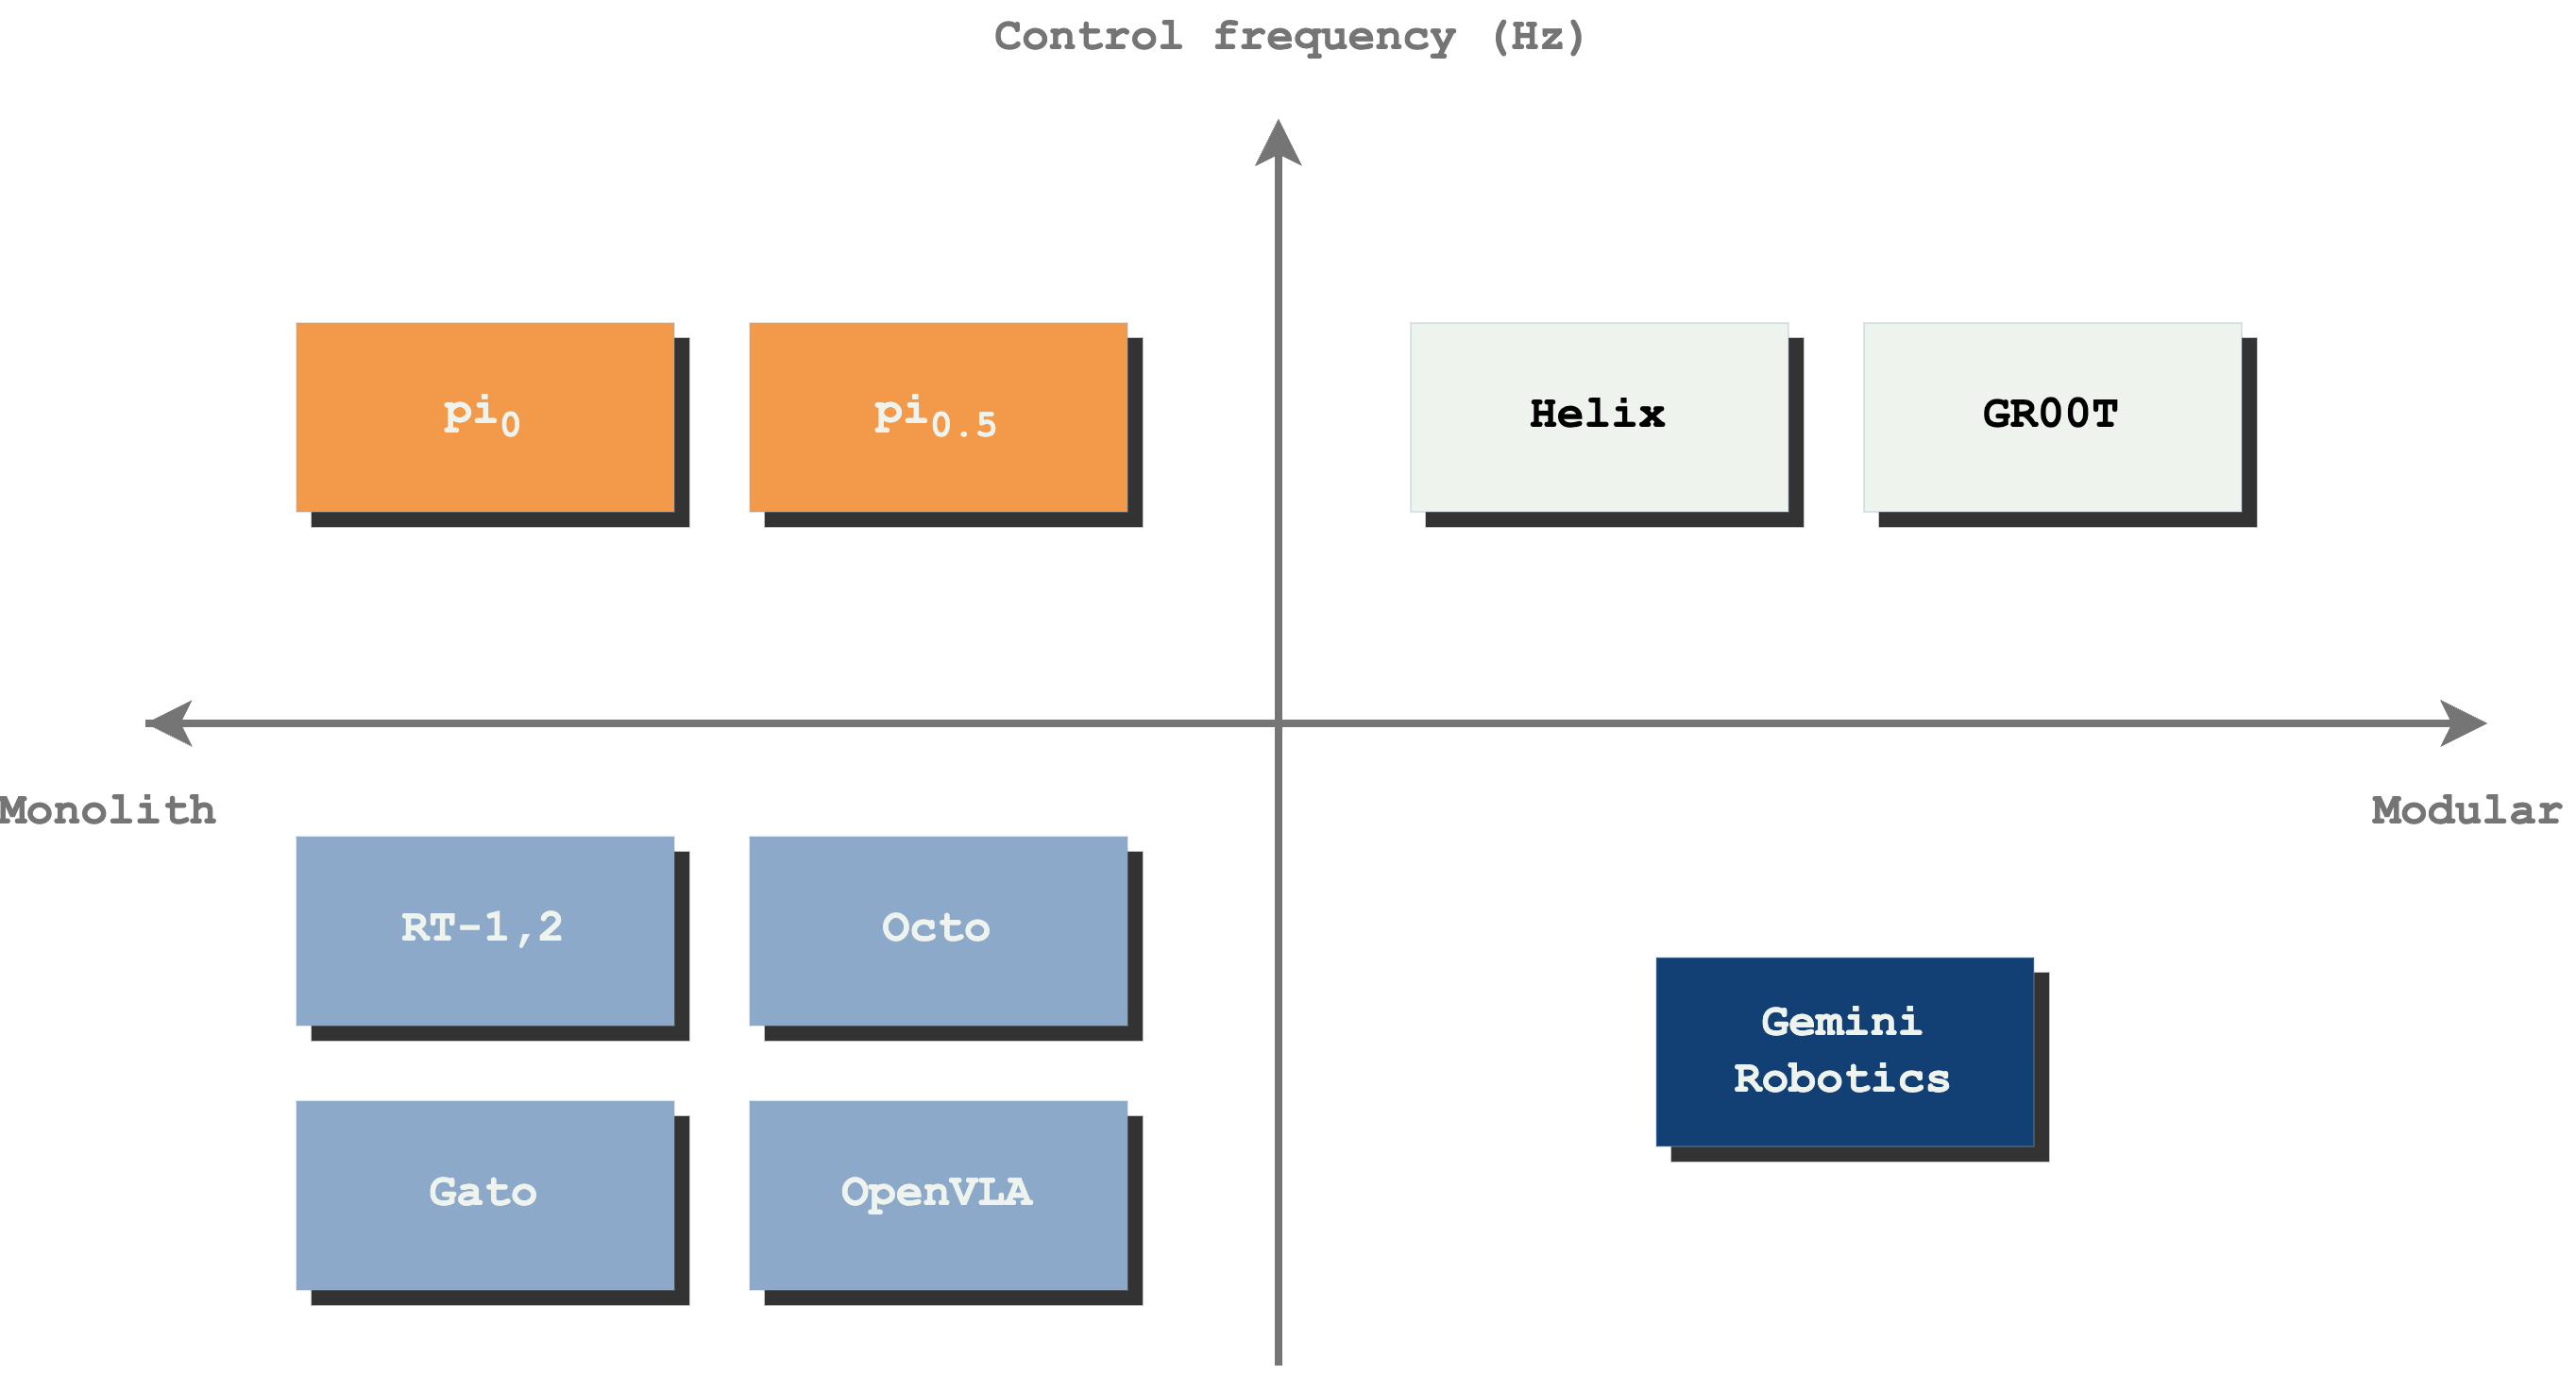
\includegraphics[width=1.0\textwidth]{Figures/taxonomy.png}
    \caption{Taxonomy of Robotic Foundation Models along the axes of Modularity (horizontal) and Control Frequency (vertical). Models in the upper half exhibit higher embodiment coupling (e.g., proprioceptive inputs, closed-loop control), while those on the right are more modular, decoupling perception, reasoning, and control.}
    \label{fig:vla-taxonomy}
\end{figure}

% TODO
% \begin{importantbox}
% Missing paragraph that ties \cref{fig:vla-taxonomy} into \cref{tab:vla_eval}...

% ... the results above show the increase in VLA realibility however they will follow a similar trajectory LLMs have... there isn't enough data to make them smart enough to be general enough to do anything a human can... this is why we need new techniques. Plug to RL.
% \end{importantbox}

\begin{widetable}[htbp]
  \footnotesize
  \begin{threeparttable}
    \caption[Real-world task success rates for VLA models]{Real-world task success rates for \ac{VLA} models. These average success rates were measured under diverse evaluation protocols and do not capture important nuances in real-world benchmarking. Differences in task definitions, completion criteria, environment variability, sensor noise, hardware configurations and quality-assurance procedures mean that values are not strictly comparable across models. Readers should interpret these rates in the context of each model's specific testing methodology.}
    \label{tab:vla_eval}

    \begin{tabularx}{\linewidth}{@{}>{\RaggedRight\arraybackslash}X l l r @{}}
      \toprule
      \tableheadline{Model} &
      \tableheadline{Avg.\ success rate (\%)} &
      \tableheadline{Model size} &
      \tableheadline{Training (steps)} \\
      \midrule
      Gato \cite{GATO2022}         & 50.0\tnote{a} & 1.18B             & 1M          \\
      RT-1 \cite{RT12022}          & 97.0\tnote{b} & 35.0M             & 130K        \\
      Octo \cite{OCTO2024}         & 72.0\tnote{c} & 93.0M             & --          \\
      RT-2 \cite{RT22023}          & 62.0\tnote{d} & 55.0B\tnote{i}    & 80K\tnote{i} \\
      Gemini Robotics \cite{GEMER2025} & 65.0\tnote{e} & --\tnote{*}   & --          \\
      OpenVLA \cite{OPENVLA2024}   & 70.6          & 7.00B             & 970K        \\
      GR00T N1 \cite{GR00T2025}    & 76.8\tnote{f} & 2.00B             & --          \\
      $\pi_{0}$ \cite{PI02024}     & 78.0\tnote{g} & 3.30B\tnote{k}    & 993M\tnote{l} \\
      $\pi_{0.5}$ \cite{PI0.52025} & 82.5\tnote{h} & 3.30B             & 993M+       \\
      \bottomrule
    \end{tabularx}

    \begin{tablenotes}[para,flushleft]
      \footnotesize
      \item[*] Not disclosed but rumored to be 1T+ parameters.\\
      \item[a] $\sim$50\% success on block-stacking of novel objects (5 held-out shapes, 200 trials each) after fine-tuning; on par with single-task expert.\\
      \item[b] $\sim$97\% on seen training tasks (700+ instructions) and $\sim$76\% zero-shot generalization to unseen instructions; tested on Everyday Robots fleet with distractors and novel backgrounds.\\
      \item[c] $\sim$72\% average across six manipulation scenarios (e.g. cable insertion, coffee making, bimanual tasks) after few-shot fine-tuning; $\sim$29\% higher than RT-1-X zero-shot and matched RT-2-X on shared tasks.\\
      \item[d] Measured on novel and unseen tasks using real-robot deployments.\\
      \item[e] Multi-task average across pick-and-place and industrial assembly on a bimanual humanoid platform.\\
      \item[f] Evaluated with few-shot demos on folding, handling, wiping.\\
      \item[g] Consolidated average across pre-training demos for stacking bowls, laundry, bussing and dryer unloading.\\
      \item[h] Similar to (g) but for dishes in sink, items in drawer, laundry and making bed.\\
      \item[i] 55B PaLI-X variant trained over 80K steps and 12B PaLM-E variant over 1M steps.\\
      \item[k] 3.3B = 3.0B \ac{VLM} + 300M action.\\
      \item[l] 993M = 903M from robot demos plus 90M steps from open datasets and task-specific fine-tuning of 1--10h per task.\\
    \end{tablenotes}

  \end{threeparttable}
\end{widetable}


\subsection{Real-World Benchmarks}

To measure progress towards general-purpose, real-world-capable robots, we require benchmarks that test both the breadth and adaptability of robotic intelligence. This section surveys existing benchmarks and proposes criteria for evaluating integrated \ac{RL}-\ac{VLA} systems, with emphasis on real-world performance.

\paragraph{Multi-Task and Generalization Benchmarks.}

Early benchmarks for generalist robots have emerged in simulation. Meta-World is a suite of 50 manipulation tasks (e.g., push button, open door) used to evaluate multi-task learning and meta-learning algorithms. A single policy’s ability to master all Meta-World tasks (and generalize to new ones) is an indicator of general-purpose skill. Another is RLBench, a library of 100+ simulated tasks with diverse tool use and settings, which provides a playground for language-conditioned policies and task generalization. Results from models like $\pi_0$ and Gato on these benchmarks show decent \textit{in-distribution} performance and some ability to adapt to withheld tasks \cite{GATO2022, PI02024}. For example, Gato was evaluated on DM Control Suite tasks and Atari games alongside robotic control, and scaling laws were studied to see performance trends across domains \cite{GATO2022}. However, simulation benchmarks, while useful, often don’t capture the noise and variability of the real world.

\paragraph{Real-World Performance Benchmarks.}

A few benchmarks explicitly target real robot generalization. One notable example is the RGB-Stacking Benchmark introduced by \textcite{PICKPL2021}, where a robot arm must learn to stack novel shapes of blocks by training on some shapes and testing on unseen ones. Gato’s evaluation on RGB-Stacking’s Skill Generalization task showed it could match a specialist policy’s success rate around $\sim$50\% \cite{GATO2022}, providing a quantitative measure of cross-generalization. There are also household task benchmarks, for instance, the BEHAVIOR benchmark (Benchmark for Everyday Household Activities in Virtual, 2021) defines 100 activities (like cleaning a table, making coffee) in simulation but with an eye towards real-world complexity; it has a concept of generalization to new object instances and environments \cite{BEHAV2021}. Some researchers have attempted these tasks on real robots like the Toyota HSR or Stretch, evaluating success in real home settings. Another emerging evaluation is open-vocabulary object manipulation: tests where a robot is asked to pick or arrange objects specified by category or attribute (possibly unseen during training). RT-2 and Helix were implicitly tested on this e.g., ``pick up the strawberry toy'' vs ``pick up the dinosaur toy'' where the latter might be novel. Embodiment transfer could also be considered a benchmark: how well a policy trained on one robot does on another with minimal adjustment (Gemini’s embodiment adaptation is a case study). A crucial piece for real-world benchmarking is measuring robustness and safety: for example, the ``Real-World RL'' suite \cite{CHRL2019} proposes metrics like how often policies fail catastrophically, how much human intervention is needed, etc. For integrated \ac{RL}+\ac{VLA}, we might want a benchmark that requires an agent to understand an instruction, then learn a new skill to fulfil it. Imagine a test where a robot is told, ``Here is a new tool, figure out how to use it to hang this picture,'' success would require comprehension (\ac{VLA}) and on-the-spot learning (\ac{RL}). While no standard benchmark yet captures this full spectrum, individual components exist that can be combined.

\paragraph{Evaluation Criteria and Research Gaps in Benchmarking.}

Current benchmarks often address either generalization \textit{or} learning, but integrated systems need both. Evaluation criteria should include: (a) Generalization to novel objects/tasks (test on things not in training data), (b) Sample efficiency/Adaptation (measure how many trials or demos needed to learn a new task to a certain performance level), (c) Multi-modality (the agent must handle vision, language and possibly other sensors), and (d) Long-horizon performance (tasks requiring many steps, where planning or subgoals are needed). A combination of simulated and real benchmarks is ideal; simulation for rapid testing and ablation, and real for ultimate validation. One gap is the lack of a widely-adopted real-world benchmark suite for generalist robots. This is partly because deploying identical evaluations on physical robots is hard (equipment differences, etc.). Some initiatives, like the REAL Competition \cite{REAL2022} or Roboturk/Robomimic datasets \cite{TURK2016}, push toward standardizing evaluation by providing common environments or datasets. Benchmarking \ac{RL}-\ac{VLA} integration might involve tasks like: follow a novel instruction that requires learning a new behavior (e.g., ``Learn to use this screwdriver to tighten a bolt'' where ``using a screwdriver'' was not in training). Success would be measured by the agent’s ability to figure it out within a limited number of tries. As research progresses, the community may define challenge tasks akin to a Robotic IQ test that spans reasoning, memory, and learning. For now, researchers rely on assembling evidence across multiple benchmarks: if a new model beats baselines on Meta-World, RGB-Stacking, and perhaps a real kitchen task, this is considered progress. In conclusion, developing better benchmarks is itself an open problem, necessary to drive the field toward truly general-purpose robotic intelligence.

\section[Generalization in Real-World Environments]{Generalization in Real-World Environments: Current State and Gaps}

While foundation models show impressive generalist capabilities in lab settings, their ability to handle the open-ended complexity of the real world is limited. This section examines the state-of-the-art in real-world capable transformer-based robotic learning and identifies gaps in generalization and online learning.

\paragraph{Robustness and Distribution Shift.}

Transformer-based policies often face a reality gap when moving from curated training data to unstructured real environments. Even the best \ac{VLA} models can struggle with \ac{OOD} scenarios i.e., situations not seen during training. For instance, a model trained on indoor tabletop manipulation might falter in a completely new setting (say, outdoors or in a cluttered home with novel object types). Generalization is typically tested by holding out some object types or task variations. As noted, Gato’s real-robot evaluation involved stacking objects of unseen shapes, where it achieved moderate success \cite{GATO2022}.

Similarly, RT-2 was demonstrated to handle some novel objects and instructions beyond its direct robot experience. However, these cases remain relatively constrained (novel combinations of familiar elements) \cite{RT22023}. Truly entirely unseen environments, with new lighting conditions, unfamiliar object categories, or unforeseen physics remain a tough challenge. The current state is that no transformer-based robotic agent can yet be deployed to any arbitrary real-world environment with reliable performance. Safety and reliability concerns also emerge: models might misinterpret unusual inputs, leading to unsafe actions. A research gap here is how to make these large models more robust to distribution shift, possibly through better simulation-to-real transfer, domain randomization, or online adaptation.

\paragraph{Lack of Online Learning and Adaptation.}

Most transformer-based policies are trained offline and then frozen (or only lightly fine-tuned) before deployment. In contrast, human and animal intelligence continuously learns from experience in real time. Current systems have little ability to improve on the fly when faced with new challenges. For example, if a robot encounters a tool it has never seen, a fixed model can only rely on its prior knowledge (which might be insufficient), whereas an ideal agent would experiment and learn about the tool. Online \ac{RL} (or other forms of continual learning) are generally absent from \ac{VLA} pipelines. This is a significant gap: without online learning, models cannot systematically improve in new environments or recover from errors by refining their policy. Some initial efforts are exploring this e.g., using \ac{RL} fine-tuning to improve pretrained \ac{VLA} models \cite{IREVLA2025} but integrating real-time learning remains an open research area. Challenges include catastrophic forgetting (learning new things without overwriting old knowledge) and safety during exploration. Thus, a crucial research direction is how to imbue transformer-based agents with online adaptation, possibly through hybrid architectures or constrained exploration that keeps the robot and its environment safe.

\paragraph{Sample Efficiency and Real-World Data Constraints.}

In real-world robotics, collecting data is expensive and time-consuming, which makes sample efficiency pivotal. Yet many transformer-based approaches demand huge datasets. \ac{VLA} models like RT-2, Gemini-ER and $\pi_o$ are enabled by internet-scale pretraining or thousands of human demonstrations \cite{RT22023, GEMER2025, PI02024}. This raises concerns: can these models generalize without such extensive data for every new situation? Current evidence suggests diminishing returns when encountering scenarios not covered by training data. For instance, Gemini Robotics needed additional fine-tuning to specialize in long-horizon tasks or new embodiments, implying that pretraining alone was insufficient for those capabilities. Moreover, models may not generalize to new embodiments (robot hardware) without retraining because the dynamics and kinematics differ. While Gemini reports some success in adapting to new robots via fine-tuning \cite{GEMER2025}, true embodiment-agnostic control remains unsolved. In summary, the current state-of-the-art transformer models mark substantial progress toward real-world robotics, but fall short in generalizing to truly novel situations, learning continuously, and minimizing data requirements. The following sections delve into specific limitations and complementary approaches addressing these issues.

\paragraph{Low-Latency Control.}

Dynamic environments demand not only robust policies but also rapid inference to close the perception-action loop. For smooth locomotion and manipulation, end-to-end latency (from sensor capture to motor command) must often fall within 2–10 ms or 100–500 Hz using $f = 1/T$, to match human-like responsiveness \cite{LOCOSURVEY2025}. Higher latencies introduce perceptible lag, degrading control stability and reducing the agent’s ability to react to unforeseen perturbations. Without real-time inference, even a well-trained model cannot generalize effectively in fast-changing settings; objects move, lighting shifts, and contacts occur unpredictably. Thus, designing transformer-based architectures or deployment pipelines that guarantee low-latency execution (via model compression, distillation, or hardware-aware optimizations) is essential for dependable real-world performance.

\newpage
\chapter{Robotic Reinforcement Learning}
\label{sec:rrl}

\epigraph{``It is comparatively easy to make computers exhibit adult level performance on intelligence tests or playing checkers, and difficult or impossible to give them the skills of a one-year-old when it comes to perception and mobility.''}{Hans Moravec \cite{MORAVEC1988}}

% \begin{importantbox}{Notes to add}
% Mentioned the focus on real-world trianing data on robots. The pro's and con's of simulation. It looks like co-trianing does produce stronger results but we need sample efficient means in the real world: SAC v PPO v TD3.
% \end{importantbox}

Building off the theoretical foundation developed in \S\ref{sec:rl_theory} now with focus on applying to \ac{RL} specifically to real robotic policies. \ac{RL} provides a complementary perspective to the largely offline-trained \ac{VLA} models. This section explores state-of-the-art \ac{RL} approaches in robotics, focusing on policy gradient methods and hybrid techniques, and briefly contrasts them with older, sample-inefficient algorithms.

\section{Policy-Gradient Methods}

\subsection{Actor-Critic}

% \epigraph{``Give me six hours to chop down a tree and I will spend the first four sharpening the axe.''}{Abraham Lincoln}

% \begin{flushright}{\slshape    
%     Give me six hours to chop down a tree and\\
%     I will spend the first four sharpening the axe.} \\ \medskip
%     --- Abraham Lincoln
% \end{flushright}

% \begin{importantbox}{Important}
%     Is this just repeating the section from elements? This should be talking more about residuals.
% \end{importantbox}

Policy gradient algorithms have become a cornerstone for continuous control in robotics. \ac{PPO} is a prime example, it's a model-free \ac{RL} method known for its stability and reliability in training complex policies \cite{PPO2017, IREVLA2025}. \ac{PPO} and related actor-critic methods (like \ac{A3C}/\ac{A2C}, \ac{DDPG}, \ac{SAC}) strike a balance between improving the policy and not deviating too far from the current policy (which can destabilize learning) \cite{A3C2016, DDPG2015, SAC2018}. In practice, \ac{PPO} has been used successfully in simulated robotics tasks and even on hardware for learning locomotion or manipulation, often achieving state-of-the-art results on benchmarks in terms of final performance. The theoretical appeal of policy gradient methods is that they directly optimize for the expected reward, which is aligned with the task goal, and can naturally handle continuous action spaces.

Methodologically, \ac{PPO} introduces a clipped objective that limits how much a policy can change per update, addressing the variance and collapse issues of earlier policy gradient attempts. In robotics, \ac{PPO} and \ac{SAC} are frequently used as baseline algorithms that provide strong performance given enough training time \cite{PPO2017, SAC2018}. Key findings include their ability to learn robust behaviors (like grasping or walking) in simulation. However, even these advanced methods often require thousands to millions of environment interactions to converge, which is a challenge for real-world use. Nonetheless, they represent the state-of-the-art \ac{RL} toolkit that any new robotic learning approach must consider, either as a competitor or a component.

% TODO
% \begin{importantbox}

% Leave the theoretical bedrock to \cref{sec:review}. Here lets mainly talk about the applications of PPO/GRPO in robotics. !IMPORTANT
% \end{importantbox}

\section{Hybrid RL Approaches}

Modern robotics research often blends pure \ac{RL} with other strategies to improve efficiency and effectiveness. One hybrid approach is rewarded imitation learning or initializing \ac{RL} with demonstration data (sometimes called warm-start or behavioral cloning initialization). This can dramatically cut down exploration time by starting the agent near a good policy. Another approach is hierarchical \ac{RL}, where a high-level policy (could be learned or hand-designed) breaks tasks into subtasks that low-level controllers execute. This can be seen as a coarse form of integration between symbolic planning and \ac{RL}. \ac{PPO} itself can be considered hybrid in the sense that it leverages a critic (value function) to guide the policy updates (actor), combining value-based and policy-based methods \cite{PPO2017}. There are also model-based \ac{RL} methods, which learn a model of the environment and plan or generate imagined experience from it. These have shown higher sample efficiency on some tasks but can struggle when learned models are inaccurate. A recent trend is combining learning-based policies with search or planning at runtime for example, using a library of learned skills and a high-level search (like in the SayCan paradigm \cite{SAYCAN2022}, where an \ac{LLM} chooses which skill to apply). In terms of algorithmic innovation, soft policy gradient methods (like \ac{SAC} \cite{SAC2018}) maintain a maximum entropy objective that encourages exploratory yet stable behavior, which has improved learning speed and robustness. The literature also explores sim-to-real transfer (domain randomization, fine-tuning in real) as a hybrid between pure learning and leveraging simulated experience. Key takeaway: The cutting edge in \ac{RL} for robotics is not one algorithm, but combinations of learning strategies that address exploration, credit assignment, and transfer, often built on the backbone of strong policy gradient methods like \ac{PPO} \cite{PPO2017}.

% \section{Real-World RL}

% \begin{importantbox}{Notes}
%    HI-SERL is the harness \cite{HISERL2024} supporting \ac{PPO}, \ac{SAC} and \ac{TD3}.

%    Must talk about: there are definitely challenges of operating in the real world, like: Sample inefficiency, Sparse rewards during long horizon tasks, Safety
% \end{importantbox}

% Lorem ipsum dolor sit amet, consectetur adipiscing elit. Sed do eiusmod tempor incididunt ut labore et dolore magna aliqua. Ut enim ad minim veniam, quis nostrud exercitation ullamco laboris nisi ut aliquip ex ea commodo consequat. Duis aute irure dolor in reprehenderit in voluptate velit esse cillum dolore eu fugiat nulla pariatur. Excepteur sint occaecat cupidatat non proident, sunt in culpa qui officia deserunt mollit anim id est laborum.

\section[Generalization in Real-World Environments]{Generalization in Real-World Environments: Current State and Gaps}

\paragraph{Sample-inefficiency.}

It's instructive to contrast the above with earlier generations of \ac{RL} that proved impractical for robotics due to sample inefficiency. Classic Q-learning and value-iteration methods (without function approximation) were limited to very small state spaces \cite{QLERN1992}. The advent of \ac{DQN} showed that neural nets could learn value functions from high-dimensional inputs, but algorithms like \ac{DQN} (and its variants) still required enormous numbers of steps (e.g., millions of frames on Atari) to learn, and extended poorly to continuous control \cite{DQN2013}. Early policy gradient algorithms like REINFORCE had high variance and typically needed careful tuning and baseline subtraction to work \cite{REINFORCE1992}. Methods like \ac{ES} or grid search over policies were even more sample-inefficient, though simpler \cite{ES2017}. In robotics, brute-force methods (like random search in policy space, or PILCO which attempted Gaussian process models) were limited by data requirements or model inaccuracies \cite{PILCO2011}. These outdated techniques are referenced for historical context: they underscore why the field pivoted to using function approximators (deep nets) and why on-policy learning alone is tough when each trial is costly. For instance, a robot hand learning to rotate an object with naive \ac{RL} could take hundreds of hours of practice, which is infeasible without simulation. Modern methods like \ac{PPO} improved stability but still rely on many trials \cite{PPO2017}; thus, much of the research has been about improving sample efficiency (via off-policy algorithms, better exploration, or leveraging prior data). Overall, the field has largely moved past pure trial-and-error learning towards more data-efficient hybrids, but the lessons from those older methods (the need for better exploration, the danger of unstable updates) inform today's algorithm design.

\newpage

\cleardoublepage
% \ctparttext{You can put some informational part preamble text here. 
% Illo principalmente su nos. Non message \emph{occidental} angloromanic
% da. Debitas effortio simplificate sia se, auxiliar summarios da que,
% se avantiate publicationes via. Pan in terra summarios, capital
% interlingua se que. Al via multo esser specimen, campo responder que
% da. Le usate medical addresses pro, europa origine sanctificate nos se.}
\labeledpart{Method}{part:method}

\chapter{Research Synthesis}
\label{sec:synthesis}

Transformer-based \ac{VLA} models have ushered robotics into an era of true quasi-generalist capability, demonstrating that a single model can, to an extent, see, reason and act across diverse tasks; yet leading examples \cite{PI0.52025, HELIX2025, GR00T2025, GEMER2025}, despite enabling zero-shot manipulation of novel objects, remain far from the master-of-all-trades that real-world deployment demands. By weaving together the threads of classical control, \ac{AI}, transformer-based foundation models, \ac{RL} and modular architectures, we synthesize these advances to shape our research approach, leveraging breadth from pre-trained models, depth from online adaptation and structure from modular design, and we highlight the gaps that must be bridged for truly adaptive robotic learning in \ac{OOD} environments.

\section{Key Insights}

\paragraph{Foundation Models Enable Breadth.}
Foundation models provide robots with a priori knowledge and generalization capabilities previously unseen in robotics. Models like RT-2 and PaLM-E demonstrate that a single model can leverage web-scale data to perform many tasks and even exhibit zero-shot behaviors \cite{RT22023,PALM2023}. This breakthrough allows handling \emph{novel inputs} (new objects or instructions) because the model likely encountered similar examples during training (e.g., RT-2 recognizing a ``coffee mug'' it never saw in fine-tuning). However, foundation models alone are not a panacea: they tend to be heavy, inflexible after training, and their real-world performance can degrade under distribution shift without further adaptation \cite{COLOSSEUM2024}.

\paragraph{RL Enables Depth.}
\ac{RL} gives robots the ability to improve with experience in new scenarios. \ac{RL} can fine-tune a policy to dynamics or reward specifics not covered in pre-training \cite{RLSURVEY2013}. It is essential for \emph{online learning}: when encountering an \ac{OOD} environment, \ac{RL} can adjust the policy incrementally. Yet \ac{RL} alone is too slow and unsafe to tackle large distribution shifts from scratch. The synergy is clear: a foundation model supplies a strong initial policy, and \ac{RL} refines that policy to the specific context efficiently \cite{PPO2017}, achieving \emph{fast adaptation} with orders of magnitude fewer trials than learning from zero.

\paragraph{Hybrid and Modular Architectures Provide a Structural Prior.}
By not relying on a single monolithic neural network, hybrid and modular architectures enforce safety, handle multi-objective trade-offs, and incorporate specialist knowledge. For example, a classical \ac{PID} loop can maintain low-level stability, and safety checks can override learned policies if a collision is imminent. Structured models often outperform end-to-end approaches in robustness \cite{CHRL2019}. Moreover, modular design aligns with practical engineering: individual modules (e.g., vision systems) can be upgraded without retraining the entire policy, which is vital for long-term system development.

\paragraph{Research Hypothesis.}
An approach that integrates a transformer-based foundation model (for generalization), \ac{RL} (for adaptation), and a modular architecture (for safety and structure) is a promising path to adaptive robotic learning. Alone, each component has limitations: foundation models without adaptation may fail under distribution shift, \ac{RL} without a strong prior is too slow, and rigid modular systems lack novelty handling. Together, they form a more complete solution.

From these insights, our research hypothesis is reinforced: an approach that integrates a transformer-based foundation model (for generalization), \ac{RL} (for adaptation), and a modular architecture (for safety and structure) is a promising path to adaptive robotic learning. None of these components alone would likely succeed: foundation models without adaptation might fail when their assumptions break, \ac{RL} without a strong prior is too slow, and a rigid modular system without learning can't handle novelty. Together, they form a more complete solution.

\section{Outstanding Gaps and Challenges}

\paragraph{Generalization vs. Specialization Balance.}
Large foundation models excel at broad generalization but can lack the precision or efficiency of smaller, specialized policies trained via \ac{RL} for specific robots and tasks. To bridge this gap, we must develop methods such as task-specific fine-tuning of large models or distilling their knowledge into compact high-frequency controllers that preserve broad capabilities while delivering task-level performance. For example, one could distill RT-2’s policy into a lightweight network optimized for real-time execution. Our research will investigate fine-tuning and distillation strategies that adapt foundation models to particular robots and environments without sacrificing their general knowledge.

\paragraph{Safety and Trustworthiness.}
Modular architectures allow embedding safety rules, yet formally verifying that a learning-enabled robot remains safe under all real-world variations is generally intractable. Control-theoretic tools (e.g., Lyapunov stability analysis) offer partial guarantees, but neural policies defy exhaustive analysis. Practical approaches include safety shields and extensive simulation under perturbations-practices we will adopt. A critical open problem is online monitoring: detecting when the robot enters an unknown regime and gracefully reverting to a provably safe baseline. We will explore anomaly-detection modules (e.g., flagging out-of-distribution sensor inputs via a generative model) to trigger safe mode, acknowledging this remains a challenging research frontier.

\paragraph{Continual Learning and Memory.}
While our current framework enables fast adaptation in a new environment, it does not ensure retention of prior skills. As a robot encounters ever more varied settings, it should accumulate competencies without catastrophic forgetting. True continual learning is unsolved: naively fine-tuning via \ac{RL} will overwrite earlier knowledge. Potential solutions include modular compartmentalization of new skills (e.g., adding task-specific subnetworks) or meta-learning schemes that consolidate parameters. We identify the stability–plasticity dilemma: maintaining performance on environment A while learning B, as a key gap. We plan experiments to measure forgetting and to test methods such as Elastic Weight Consolidation or orthogonal gradient descent for mitigating it.

\paragraph{Benchmarking and Evaluation.}
There is currently no standard benchmark for ``adaptive robotics.'' In this thesis we take a first step by introducing a structured real-robot evaluation protocol, but more broadly we argue that the community should develop a comprehensive evaluation suite drawing on modified Meta-World tasks, Colosseum-style real-world perturbation tests, and sensor-failure scenarios to measure adaptation across sensor, environment, and task changes. Such a protocol, spanning new objects, varied terrain, and shifting goals, would provide breadth and consistency and could serve as a shared benchmark for fair comparison.

\section{Synthesis for Approach}

Considering all of the above, we synthesize the approach as follows: We will start with a strong foundation (a pretrained transformer model endowed with multimodal understanding) and anchor it to a reliable control backbone (ensuring baseline competence and safety). On this foundation, we will layer an adaptation mechanism (\ac{RL} fine-tuning or online learning) that refines performance in novel scenarios. The expected outcome is a robot that, upon encountering an \ac{OOD} situation, initially behaves reasonably (not randomly, thanks to the foundation model) and then improves rapidly through experience (thanks to \ac{RL}), all while never venturing into catastrophic behavior (thanks to safety modules and constraints).

By iteratively testing this system on increasingly challenging distribution shifts, we will validate the core hypothesis. Success will be measured by the robot’s ability to maintain high task success with minimal drop after a shift and how quickly it can recover any lost performance. For example, if introducing a 30\% perturbation in the weight of an object causes the success to drop from 90\% to 50\%, can our system learn to return, say, 80\% + success in a small number of trials? Does it avoid dangerous attempts during that adjustment?

The literature gives optimism that each piece can achieve parts of these goals: foundation models have shown the ability to do things like pick up unfamiliar objects correctly on the first try, and meta-\ac{RL} has shown fast improvement within tens of trials on new tasks in simulation. The novel contribution of our work will be to seamlessly integrate these pieces in real robotic hardware and demonstrate end-to-end that the robot can take what it ``knows'' (from pre-training) and adapt what it does not (through experience), in a unified system.

In the next section, we transition from what needs to be done to how we will do it. We outline the concrete research questions we will answer and the experimental methodologies, metrics, and implementation steps that will operationalize this synthesized approach.
\newpage
\chapter{Methodology}
\label{sec:method}

\section{Formulated Research Questions}
\label{sec:rqs}

Drawing on the synthesis from \cref{sec:synthesis}, we set out four focused research questions that shape the experimental design. Each question links a concrete objective with a testable hypothesis and identifies the key methodological lever or research gap it addresses.

\begin{enumerate}
    \item \textbf{RQ1: To what extent does a transformer-based foundation model pre-trained on broad data generalize to novel robotic tasks and unseen environments?}\\[2pt]
    \textit{Objective}: Quantify zero-shot and few-shot success, failure modes and transfer gaps across varied manipulation tasks.\\[2pt]
    \textit{Hypothesis}: The model will handle moderate perceptual changes yet falter when action dynamics or task semantics shift significantly.

    \item \textbf{RQ2: Can online \ac{RL} fine-tuning restore or surpass baseline performance after large distribution shifts within tens of physical trials, and which fine-tuning strategy is most efficient?}\\[2pt]
    \textit{Objective}: Compare full-model versus partial-layer updates, on-policy versus off-policy data and safety-aware reward design. Record trials-to-recovery and asymptotic performance.\\[2pt]
    \textit{Hypothesis}: With a strong initialization from the foundation model and possibly demonstration data as a warm start, \ac{RL} adaptation will achieve substantial improvement in tens of episodes rather than thousands, representing a significant gain in sample efficiency.

    \item \textbf{RQ3: Do modular architectures that divide fast low-level control from slower high-level reasoning yield more robust real-time behavior than monolithic policies?}\\[2pt]
    \textit{Objective}: Benchmark a two-tier controller (embedded ``cerebellum'' at 200–500 Hz, cloud planner at 1–10 Hz) against an end-to-end baseline under latency, sensor noise and obstacle perturbations.\\[2pt]
    \textit{Hypothesis}: The modular design will sustain task success under latency stress whereas the monolith will degrade.

    \item \textbf{RQ4: What communication abstraction between modules best preserves global optimality while allowing independent retraining of sub-networks?}\\[2pt]
    \textit{Objective}: Evaluate interfaces such as shared latent spaces, explicit symbolic messages and probabilistic belief states in simulated pick-and-place and long-horizon assembly tasks. Measure learning stability, sample efficiency and retrain cost.\\[2pt]
    \textit{Hypothesis}: A compact stochastic latent protocol aligned with information-bottleneck theory will minimize retrain overhead while maintaining overall performance.
\end{enumerate}

This honours thesis investigates \textbf{RQ2} within the available timeframe. RQ1, RQ3 and RQ4 define the broader research landscape and motivate future work.

\section{Experimental Platform}

\subsection{Robotic Hardware}

The robotic hardware used for all real-world experiments is summarized in the tables in this section and illustrated by the STL layouts in \cref{fig:robot_parts}, the assembled SO-101 manipulators in \cref{fig:so101}, and the complete tabletop setup in \cref{fig:experimental_platform}. For real-world experiments, a physical SO-101 3D-printed robotic arm was used as the manipulator, as shown in \cref{fig:so101} \graffito{A complete material list can be found in \cref{tab:so101_bom}.}. The arm is a teleoperated tabletop platform with three rotational degrees of freedom and a parallel gripper, rigidly mounted to a flat work surface. Visual observations of the workspace were provided by fixed external RGB cameras positioned to capture both the robot and the task area. All control, data recording, and policy inference were performed on a desktop computer equipped with a consumer-grade NVIDIA RTX 3080 and RTX 5080 \acp{GPU}. Variations in the tabletop environment and object set across tasks introduced distribution shifts in object geometry and mass, surface friction, clutter, and camera viewpoint, providing a range of real-world conditions for evaluation.

\begin{figure}[ht]
    \centering
    \subfloat[Leader robot components\label{fig:leader_parts}]{
        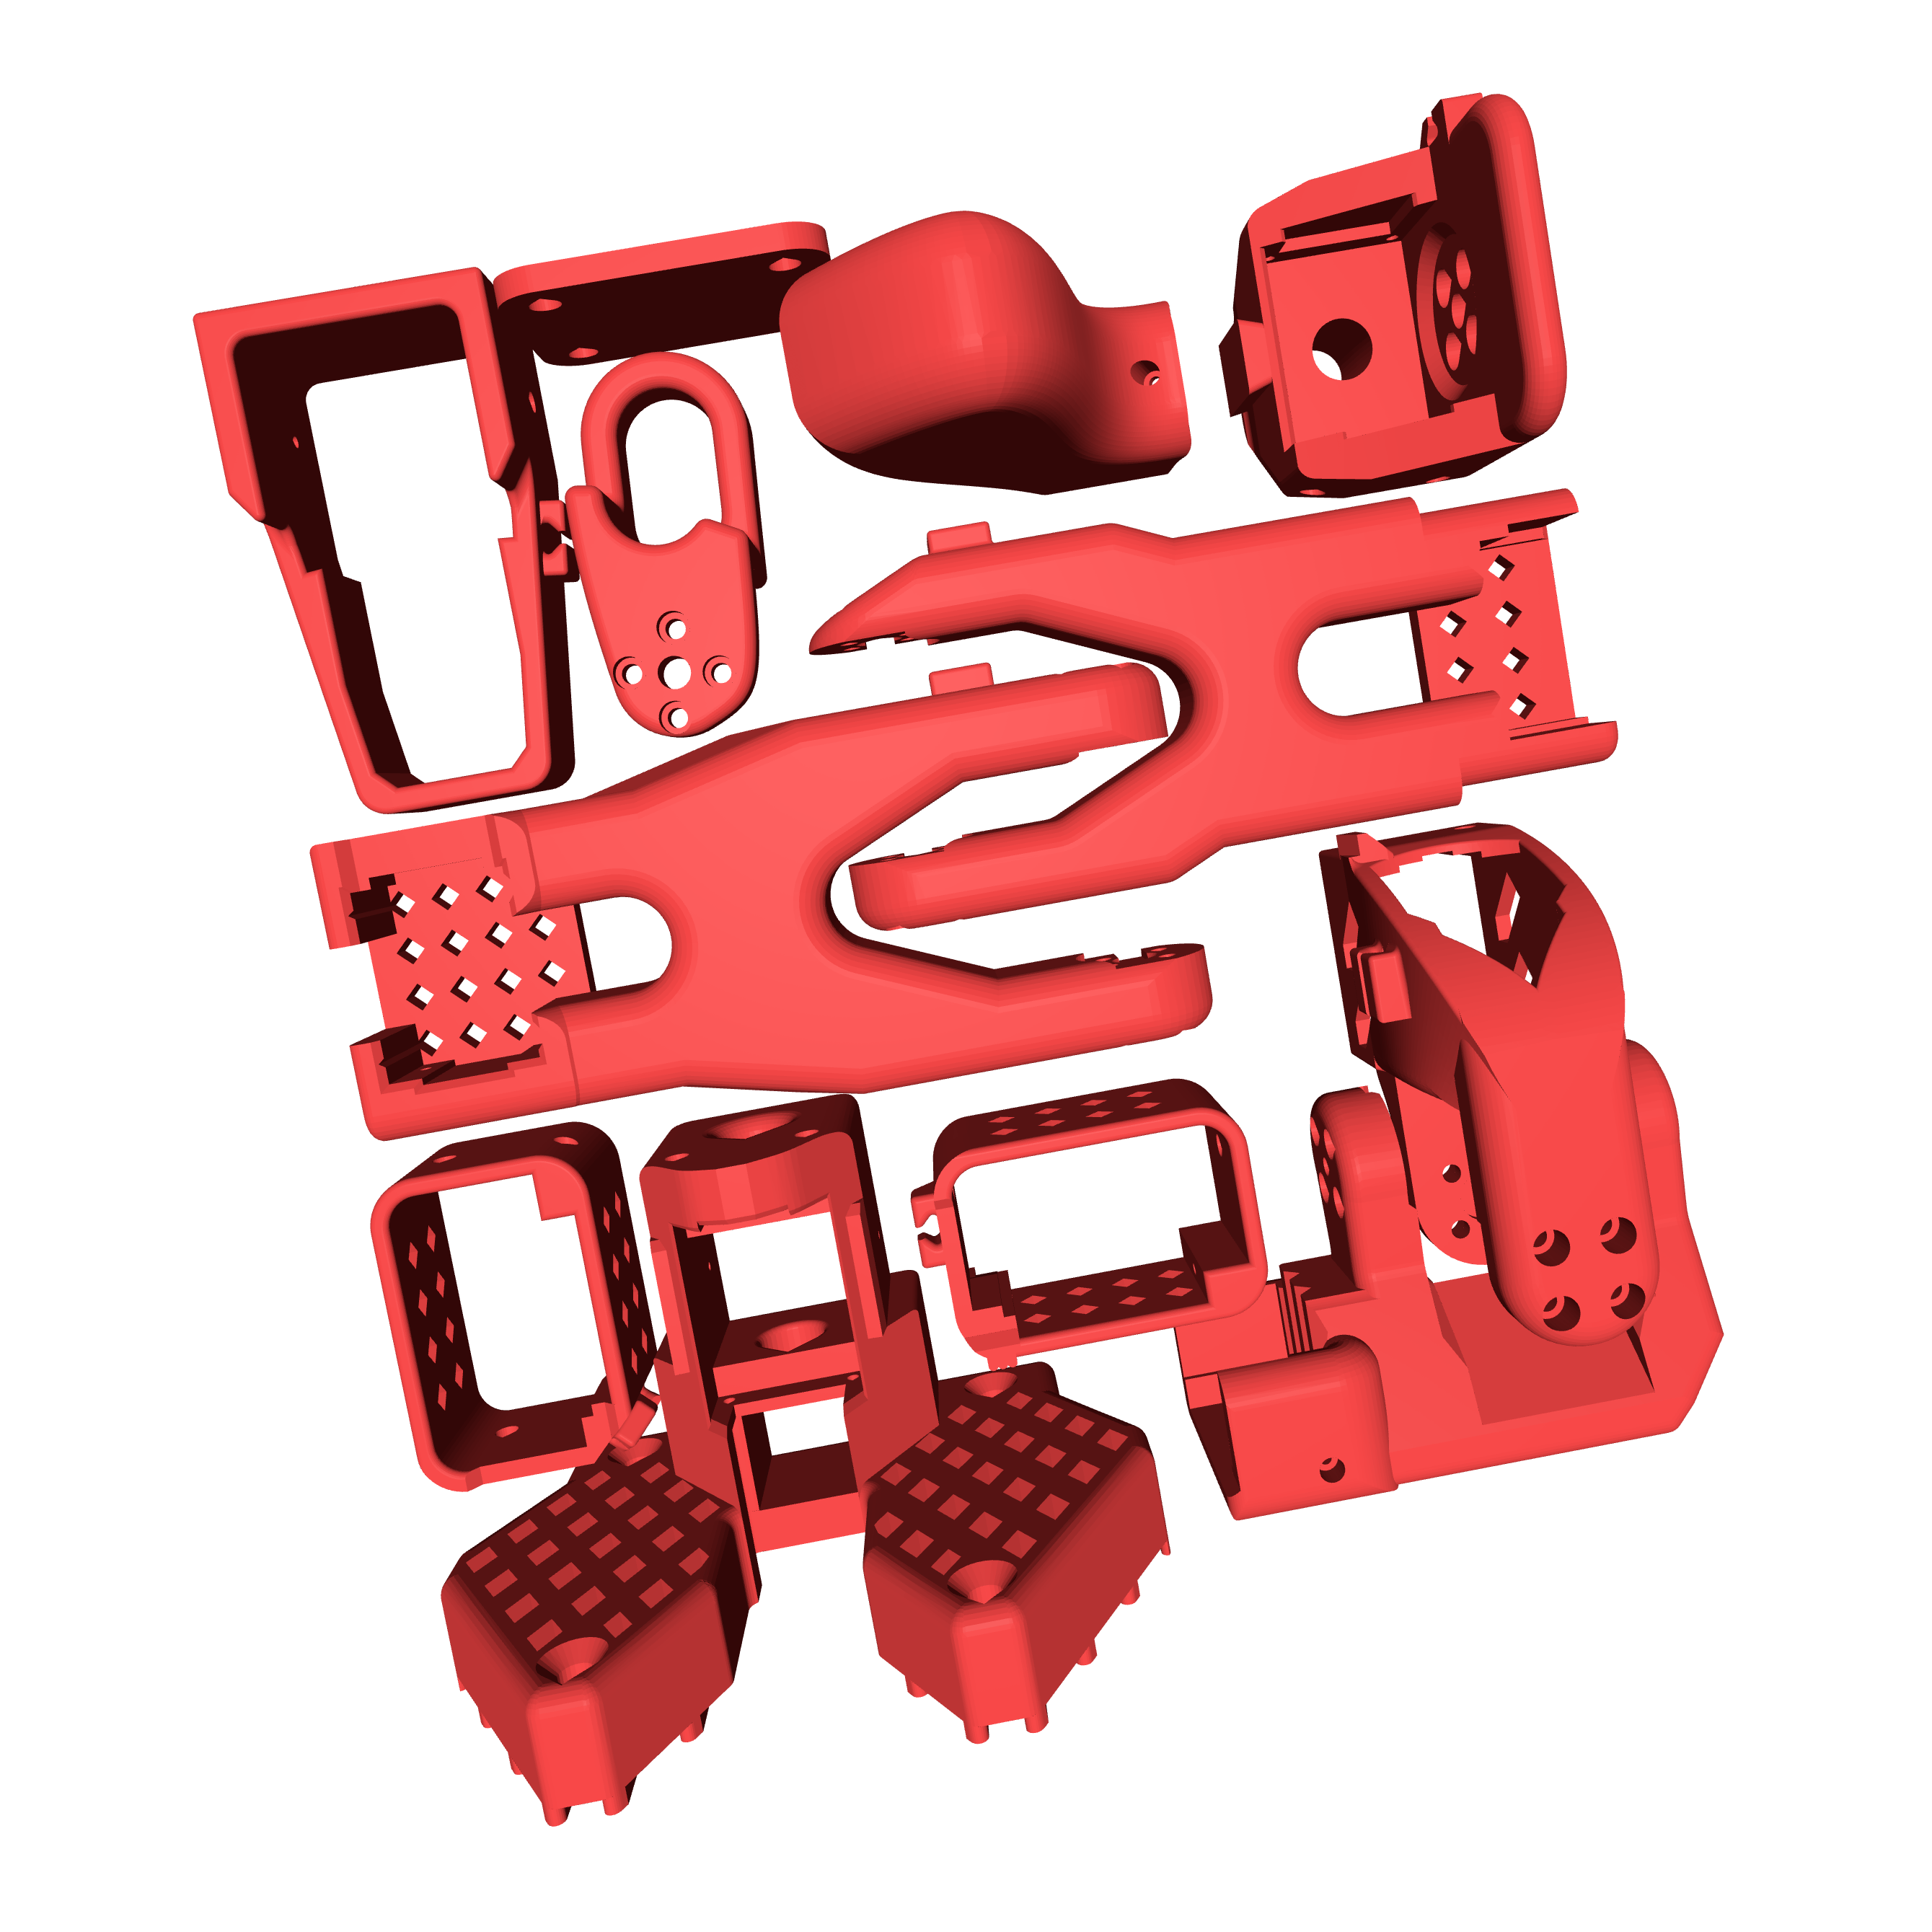
\includegraphics[width=0.45\linewidth]{Figures/leader_parts.png}
    }\hfill
    \subfloat[Follower robot components\label{fig:follower_parts}]{
        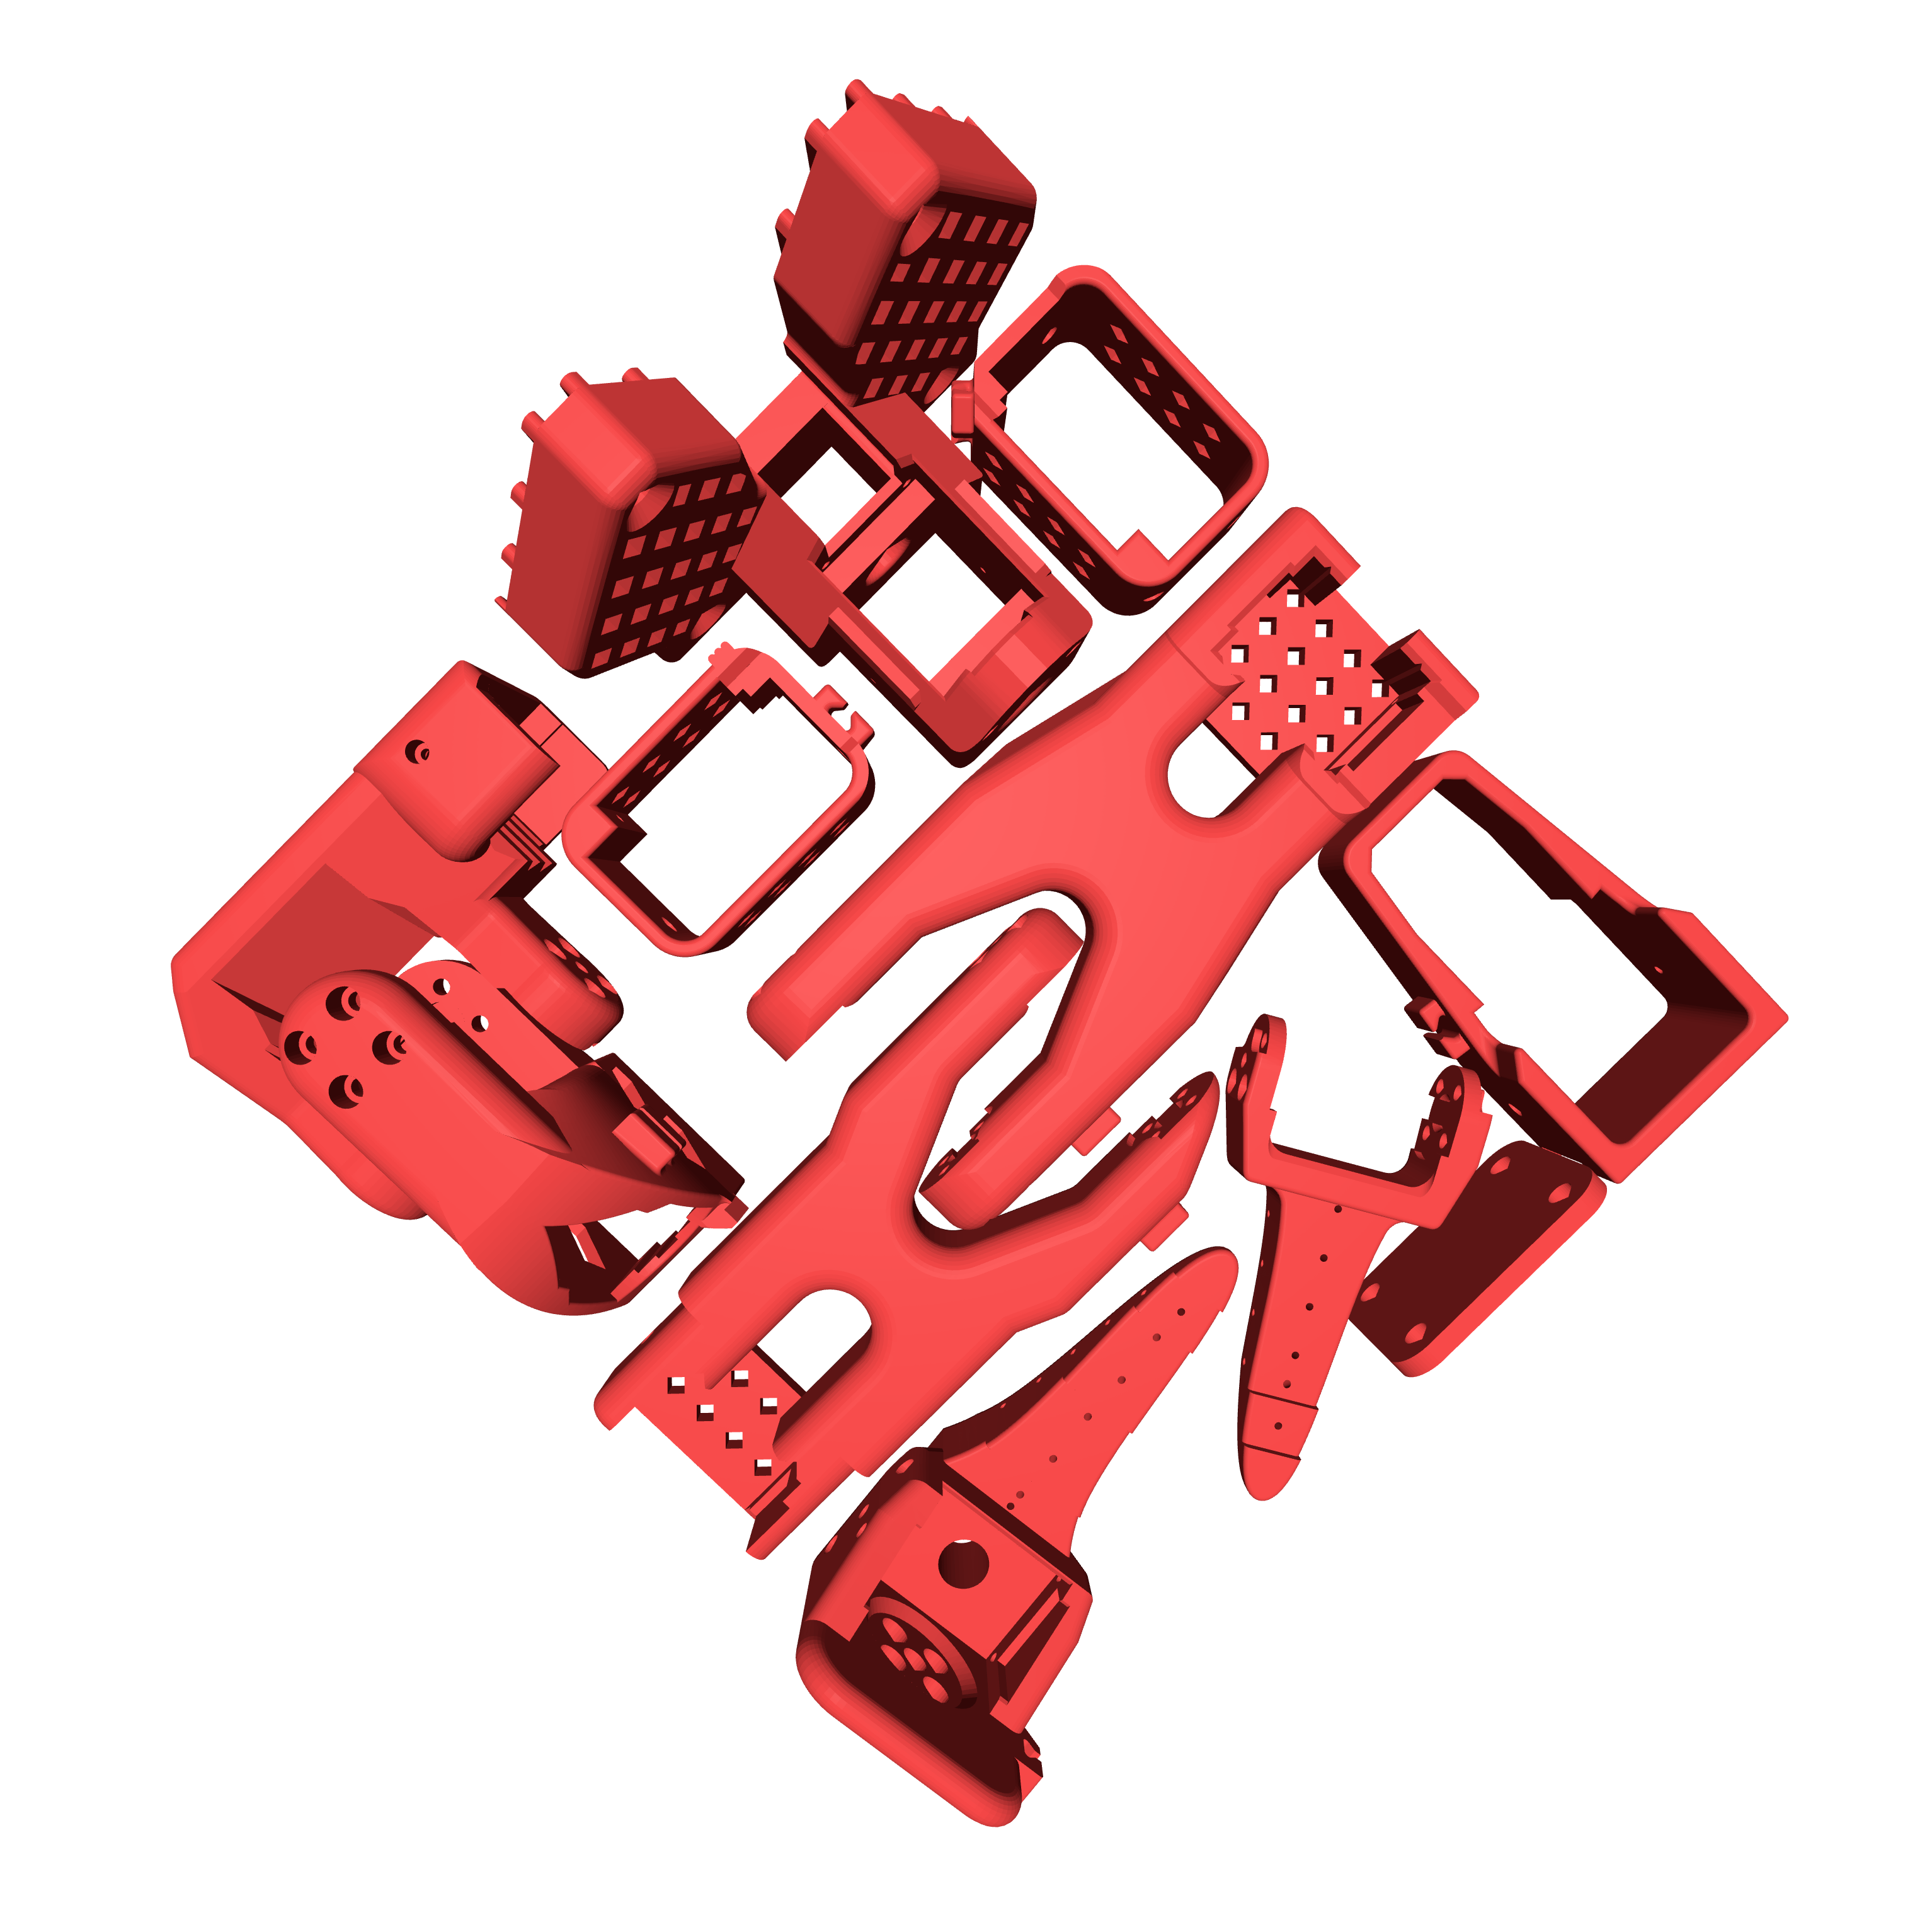
\includegraphics[width=0.45\linewidth]{Figures/follower_parts.png}
    }
    \caption{STL layouts of the leader and follower robot components arranged on the Ender 3 printer bed for fabrication.}
    \label{fig:robot_parts}
\end{figure}

\begin{figure}[ht]
    \centering
    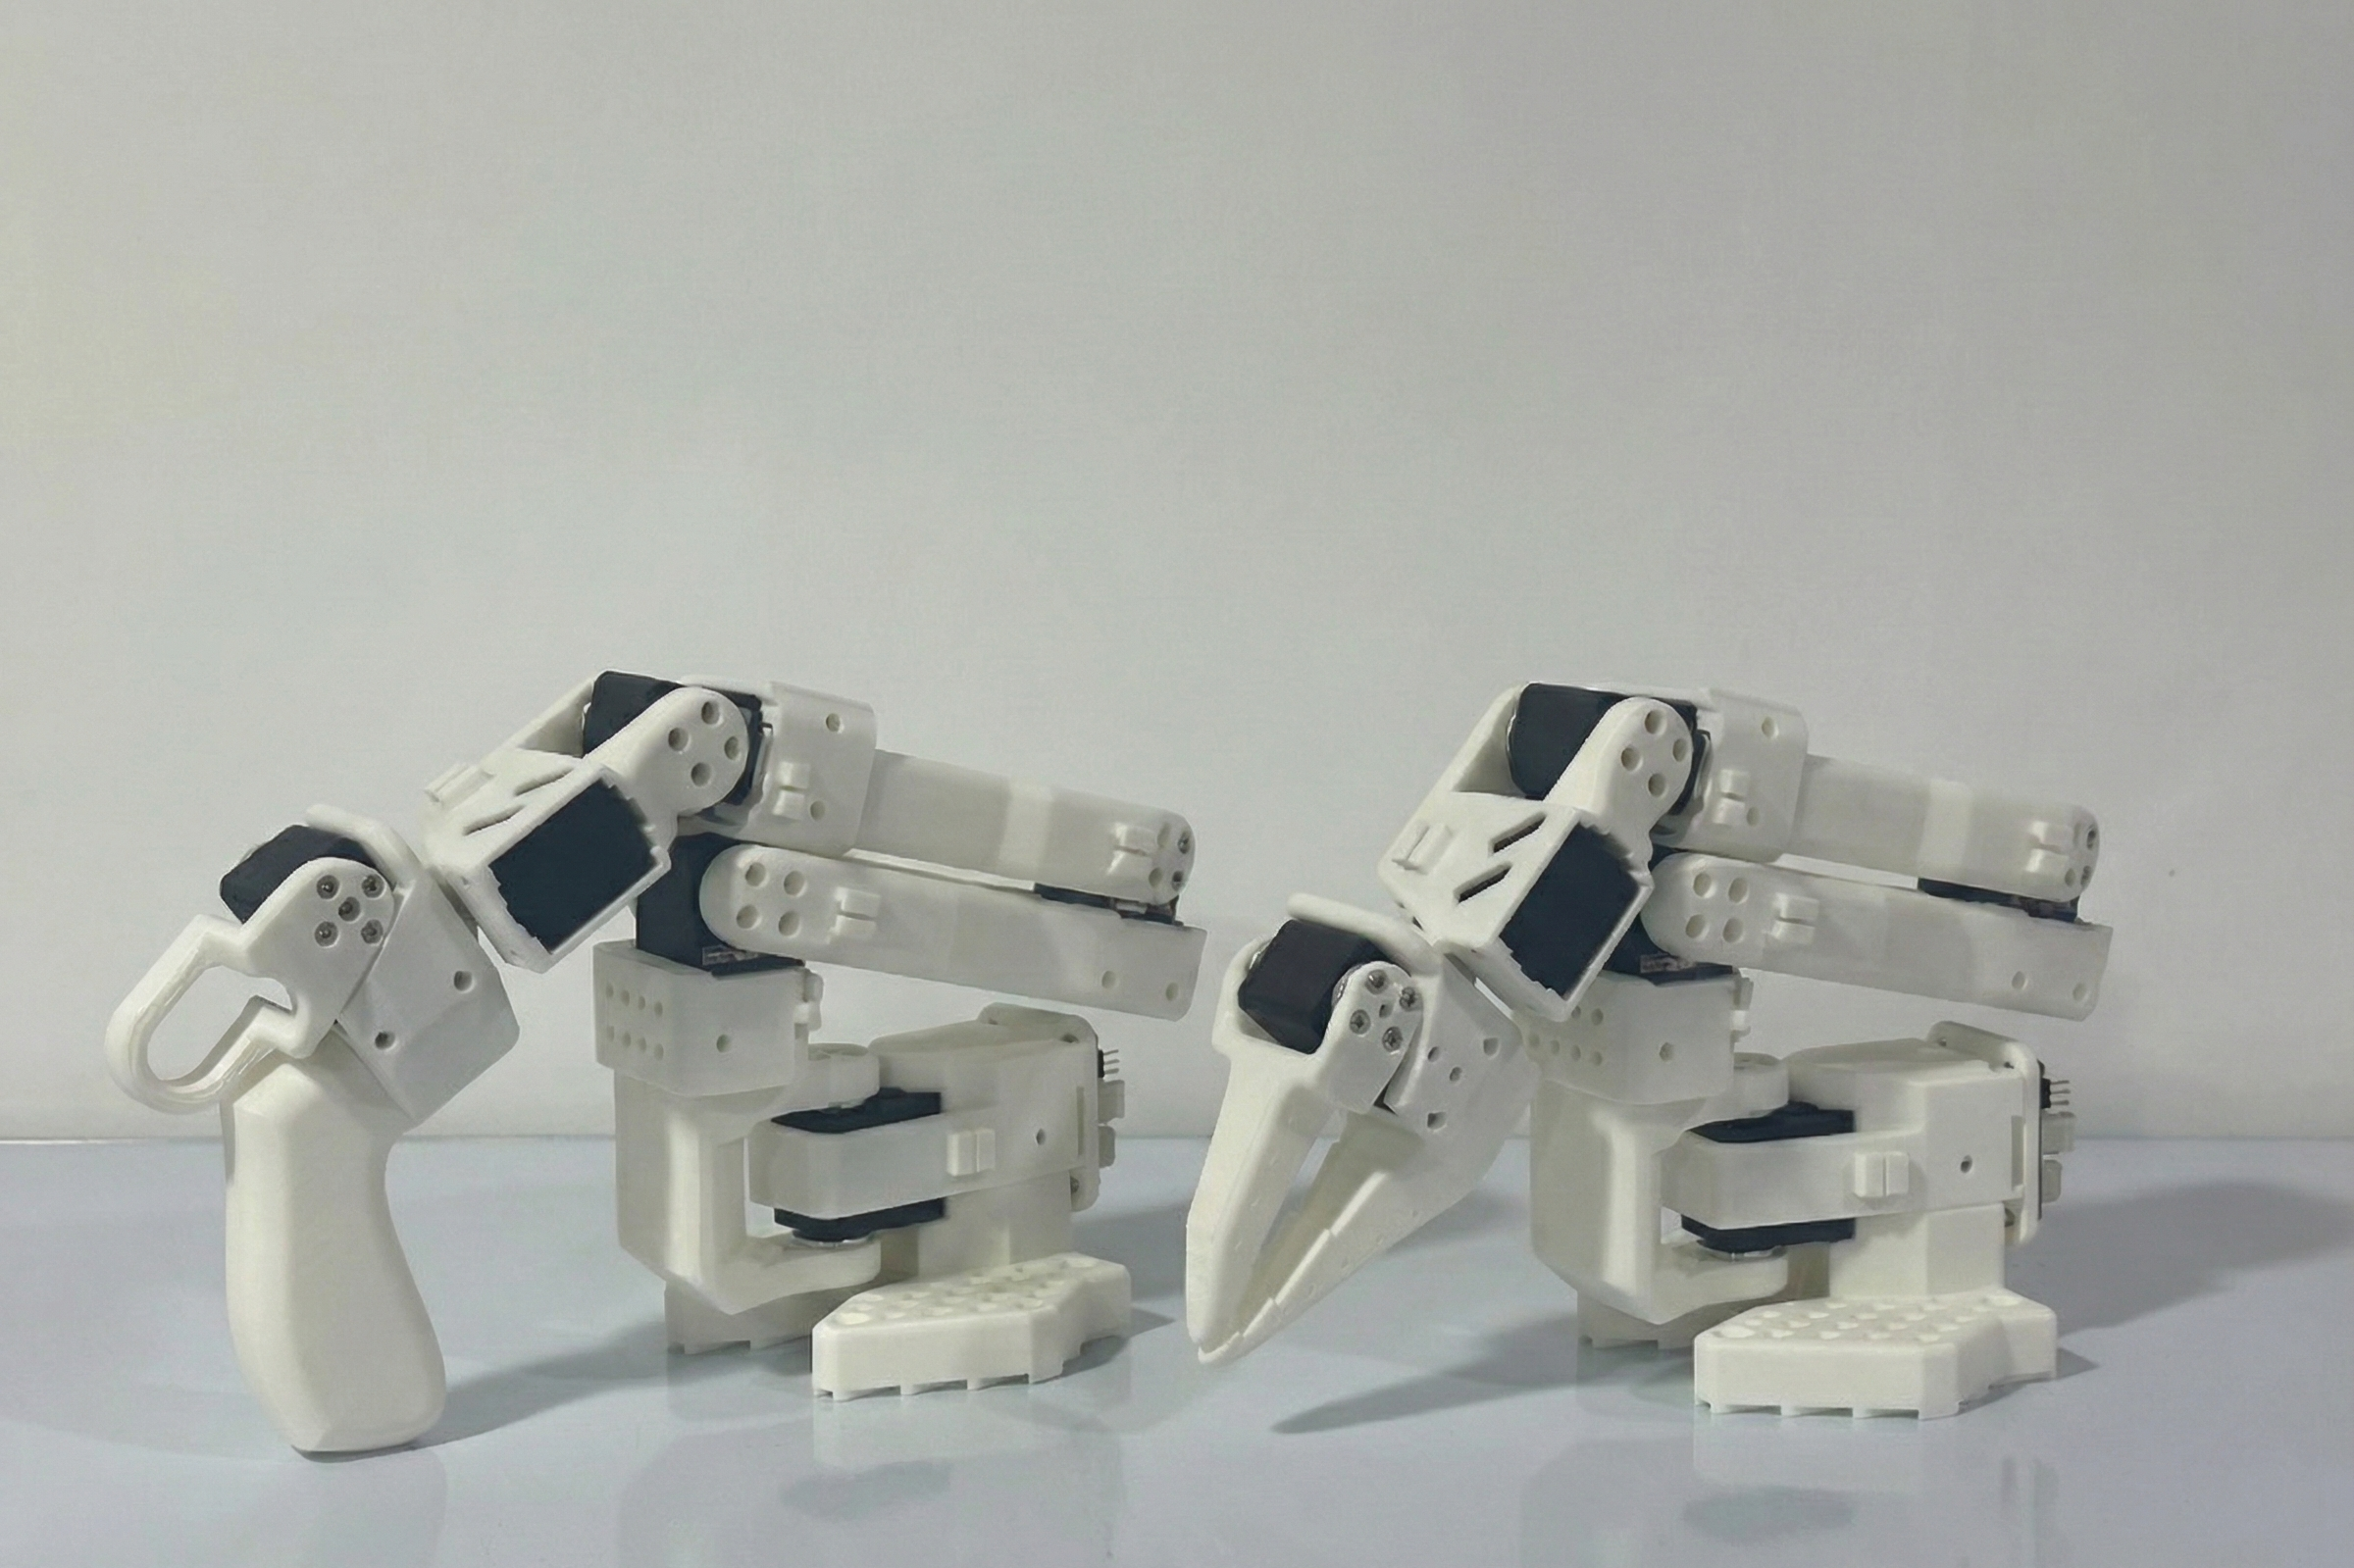
\includegraphics[width=1.0\linewidth]{Figures/so101-arms.png}
    \caption{A pair of white 3D-printed SO-101 robotic arms with black ST-3215-C0xx servos, resting side-by-side on a clean white surface.}
    \label{fig:so101}
\end{figure}

\begin{figure}[ht]
    \centering
    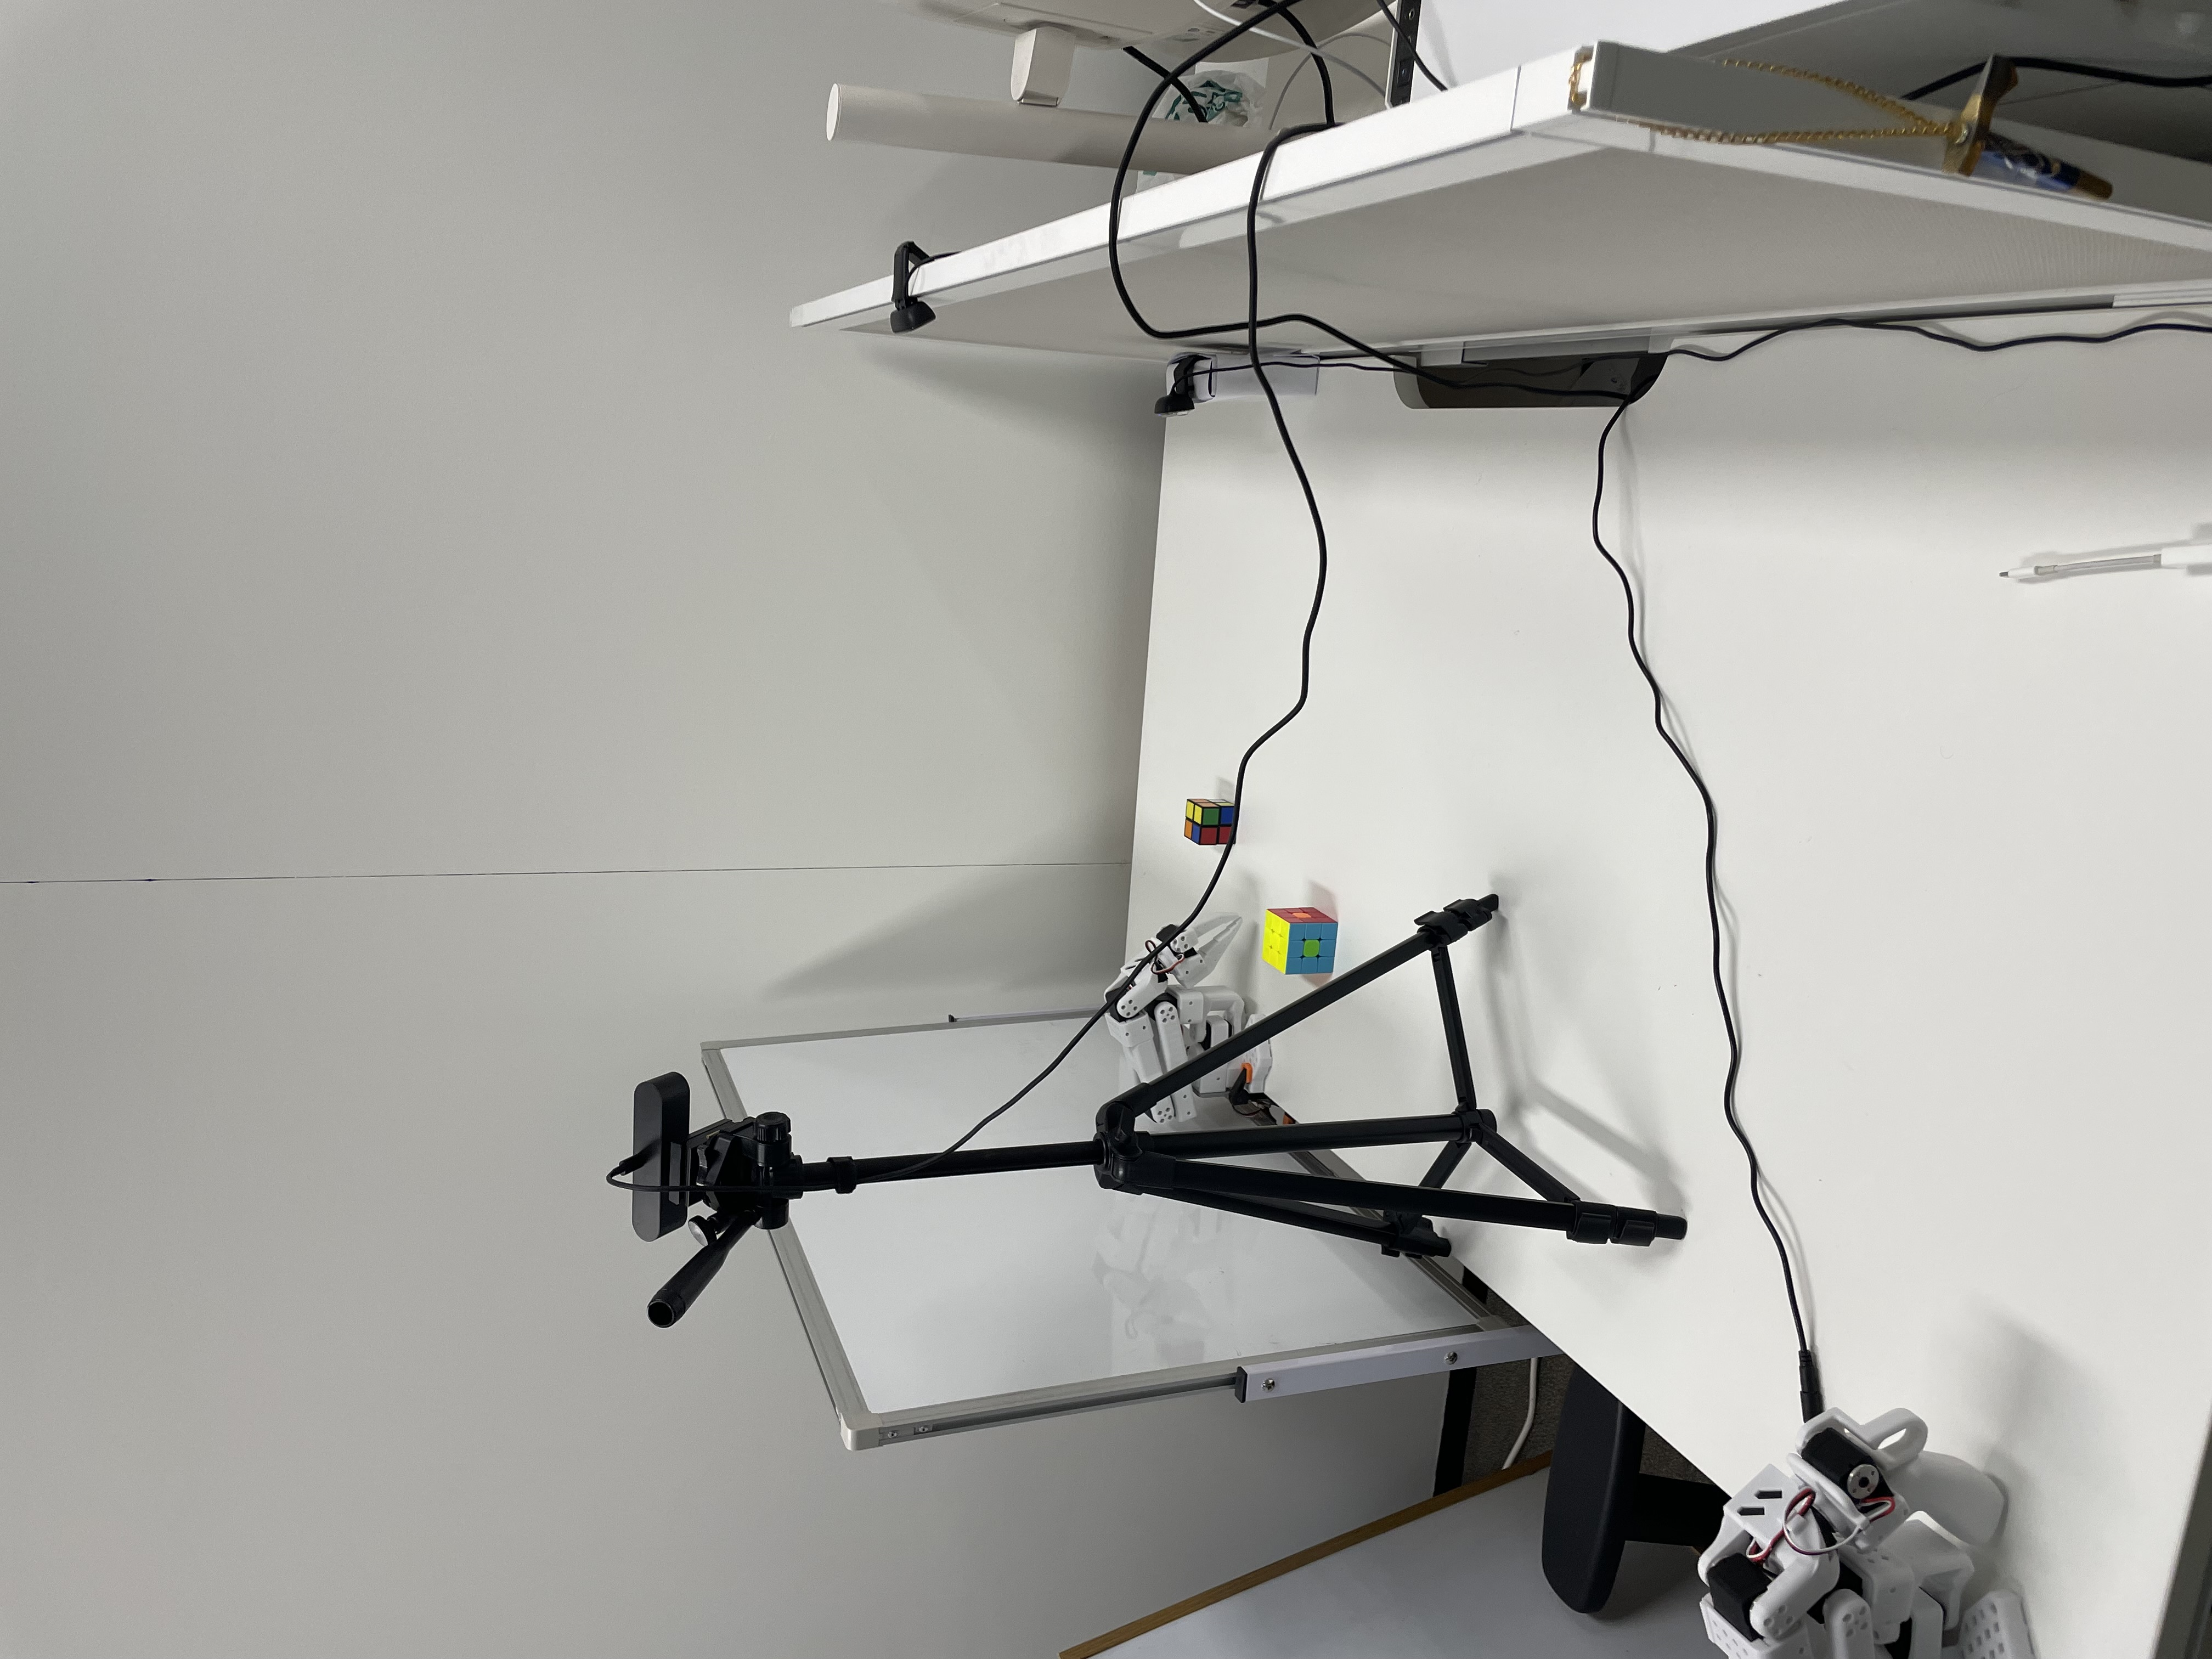
\includegraphics[width=\textwidth,angle=270]{Figures/experiment-setup.jpg}
    \caption{Experimental tabletop manipulation setup with a Lenovo top camera mounted on a tripod providing an overhead view of the white workspace, a front facing Microsoft LifeCam attached to the desk divider, and a Logitech auxiliary camera used for task monitoring, reward computation, and partitioning the workspace into discrete zones to curate balanced and diverse training data. A 3D printed SO-101 robotic arm and gripper operate on a colored training cube and a Rubik's cube on the central table, with whiteboards, an office chair, and USB cables routing connectivity between cameras and the control machine.}
    \label{fig:experimental_platform}
\end{figure}

\subsection{Sensing and Vision System}
\label{sec:method:vision_system}

The sensing and vision system was designed to provide visually simple, low-clutter observations to the visuomotor backbone and residual \ac{RL} adapters. Experiments were conducted in a predominantly white office environment with minimal background texture, including whiteboard panels placed directly behind the main manipulator to create a uniform backdrop, as visible in \cref{fig:so101,fig:experimental_platform}. This configuration reduces background clutter and high frequency visual noise, which can otherwise induce spurious correlations when policies are trained directly on pixel observations and lead to brittle behaviour under small appearance changes.

The primary camera configuration consists of a top camera mounted on a tripod that provides an overhead view of the workspace and a front facing camera attached to the desk divider, as illustrated in \cref{fig:experimental_platform}. The front camera captures lateral motions of the SO-101 arm and interactions across the horizontal extent of the task space, while the top camera supplies a bird's eye view that localises both the arm and the objects on the table with minimal occlusion. Multiple alternative camera placements were evaluated, including single front views and oblique side views\graffito{All cameras were running at the recommended 30 FPS \cite{HFHUBTUT2025}.}. These alternatives frequently suffered from occlusions when the arm or gripper passed between the camera and the objects, which degraded grasp accuracy and increased the rate of failed manipulations.

An auxiliary camera, also shown in \cref{fig:experimental_platform}, is used for task monitoring, reward computation, and partitioning the workspace into discrete zones to curate balanced and diverse training data, as illustrated in \cref{fig:partitioned_workspace}. Separating this monitoring stream from the main observation views allows the same physically fixed camera geometry to serve both control and data curation, while maintaining a consistent, noise reduced visual input for policy learning and evaluation.

\bigfigure[
    pos=ht,
    opt={width=\linewidth},
    label={fig:partitioned_workspace},
    shortcaption={Top-down view of the partitioned workspace grid.}
]{Workspace/workspace-grid.png}
{Top down view from the auxiliary monitoring camera with the workspace partitioned into a discrete grid using opencv \cite{OPENCV2000}. The zone indices are used to balance data collection across object positions and interaction regions for reward computation and dataset curation.}


\subsection{Computing Infrastructure}

All real time inference for Isaac-Gr00t and the residual \ac{RL} adapters runs on a local Linux workstation equipped with NVIDIA RTX 3080 and RTX 5080 \acp{GPU}. Initial experiments on the RTX 3080 (10\,GB VRAM) led to frequent crashes and unstable robot behaviour, as Isaac-Gr00t alone required at least 8\,GB of VRAM and left insufficient headroom for system and logging processes as displayed in \cref{tab:gpu_vram}. As a result, all final real robot experiments were executed on the RTX 5080, which provided enough memory headroom to ensure stable policy execution and reliable teleoperation. The workstation also hosted the LeRobot control stack and data logging pipeline, recording synchronized camera streams, proprioceptive states, and actions for analysis.

\begin{table}[H]
    \myfloatalign
    \scriptsize
    \begin{threeparttable}
        \caption[GPU VRAM, device counts, and cloud cost]{GPU VRAM, devices per job, and indicative cloud cost used in this work.}
        \label{tab:gpu_vram}
        
        \begin{tabular*}{\textwidth}{@{\extracolsep{\fill}} l r r r @{}}
            \toprule
            \tableheadline{GPU Model} & \tableheadline{VRAM} & \tableheadline{GPU per job} & \tableheadline{Cost per job hr (USD)} \\ 
            \midrule
            RTX~3080\tnote{a} & 10\,GB & 1 & 0.00\tnote{b} \\ 
            RTX~5080 & 16\,GB & 1 & 0.00\tnote{b} \\ 
            RTX~4090 & 24\,GB & 1 & 0.00\tnote{b} \\ 
            A100     & 40\,GB & 2 & 0.06996 \\ 
            \bottomrule
        \end{tabular*}
        
        \begin{tablenotes}
            \footnotesize
            \item[a] Isaac Gr00t requires $\ge$8\,GB of VRAM for inference. The 10\,GB capacity of the RTX~3080 operates near saturation when accounting for OS overhead and auxiliary processes.\\
            \item[b] Zero marginal cost incurred as these devices were pre-owned by the author or affiliates.
        \end{tablenotes}
    \end{threeparttable}
\end{table}

All learning of residual policies and value functions was performed remotely on Modal Cloud \cite{MODAL}. Training jobs were launched via the Modal SDK (see \cref{lst:modal}) and used two NVIDIA A100 \acp{GPU} per run, enabling efficient batched rollouts and gradient updates over the collected SO-101 trajectories. This separation of concerns placed computationally intensive training on scalable cloud hardware while reserving the local workstation for low latency control and high fidelity data capture on the physical robot.

\begin{lstlisting}[float=ht,language=Python,frame=tb,
caption={Minimal Modal SDK entrypoint that launches a two A100 cloud training run from a single \texttt{modal run train.py} command.}, label=lst:modal]
@app.function(gpu="A100:2")
def train():
  # training logic
  pass

@app.local_entrypoint()
def main():
  train.remote()
\end{lstlisting}

\subsection{Datasets and Pretraining}

Datasets are collected exclusively on the physical SO-101 3D printed arm using the HuggingFace LeRobot platform, which provides a unified interface for logging observations, actions, and task metadata. No third party robot datasets are incorporated, in order to avoid mismatches in camera geometry, sensing quality, and embodiment between this setup and external collections. For each manipulation task, a set of teleoperated demonstrations is recorded and then augmented with additional on robot rollouts generated during online learning. All trajectories share a consistent, calibrated camera configuration for the SO-101 workspace, together with proprioceptive state and low level control commands.

The visuomotor backbone is the pretrained Isaac-Gr00t policy, used in its publicly released configuration. No additional pretraining of Isaac-Gr00t is performed in this work. Learning is instead restricted to lightweight residual adapters and value functions that are trained on top of the frozen backbone using the task specific trajectories described above. Perception and instruction grounding capabilities therefore originate from Isaac-Gr00t's upstream pretraining, while the collected SO-101 dataset is used solely to specialise behaviour to the target hardware and task distribution.

\subsection{Control Architecture and Software Stack}

The control architecture is built on top of the LeRobot framework \cite{LEROBOT}, which provides a unified software stack for kinematics, low level control, and data logging for the SO-101 arm. High level components specify desired end effector poses or joint targets, while LeRobot handles conversion to hardware compatible commands and enforces joint limits and velocity constraints before streaming actions to the embedded controllers.

Geometric reasoning is implemented through a dedicated \texttt{RobotKinematics} module that wraps the \texttt{placo} library for both forward and inverse kinematics, as illustrated in \cref{lst:robot-kinematics}. The solver loads the SO-101 URDF, fixes the base, and defines a frame task at the \texttt{gripper\_frame\_link}. Forward kinematics takes joint angles in degrees, converts them to radians, updates the internal robot model, and returns a 4x4 transformation of the end effector in the world frame. This representation is used for logging, visualization, and defining Cartesian targets.

\begin{lstlisting}[float=ht,language=Python,frame=tb,
caption={Skeleton of the \texttt{RobotKinematics} helper used in the LeRobot stack. Forward and inverse kinematics run in the same URDF joint space used for control and joint limit enforcement.},
label=lst:robot-kinematics]
class RobotKinematics:
    def __init__(self, urdf_path: str,
                 target_frame_name: str = "gripper_frame_link"):
        import placo, numpy as np
        self.robot = placo.RobotWrapper(urdf_path)
        self.solver = placo.KinematicsSolver(self.robot)
        self.solver.mask_fbase(True)
        self.joint_names = list(self.robot.joint_names())
        self.tip_frame = self.solver.add_frame_task(
            target_frame_name, np.eye(4)
        )

    def forward_kinematics(self, q_deg):
        import numpy as np
        q_rad = np.deg2rad(q_deg[: len(self.joint_names)])
        for name, q in zip(self.joint_names, q_rad):
            self.robot.set_joint(name, q)
        self.robot.update_kinematics()
        return self.robot.get_T_world_frame("gripper_frame_link")

    def inverse_kinematics(self, q_deg, T_target):
        import numpy as np
        q_rad = np.deg2rad(q_deg[: len(self.joint_names)])
        for name, q in zip(self.joint_names, q_rad):
            self.robot.set_joint(name, q)
        self.tip_frame.T_world_frame = T_target
        self.solver.solve(True)
        self.robot.update_kinematics()
        q_sol = [self.robot.get_joint(n) for n in self.joint_names]
        return np.rad2deg(q_sol)
\end{lstlisting}

Inverse kinematics receives the current joint configuration and a desired 4x4 end effector pose, then uses \texttt{placo}'s \texttt{KinematicsSolver} to compute a new joint configuration. Position and orientation weights allow trading off strict pose tracking against more flexible solutions that prioritize positional accuracy over orientation when needed. The resulting joint angles are converted back to degrees, and any additional gripper joints are preserved from the input vector. In practice, this kinematics layer enables LeRobot policies and teleoperation commands that are expressed in task space to be executed as smooth joint space trajectories on the physical arm.

\subsection{Teleoperation Interface and Data Collection Pipeline}

Demonstration data are collected using LeRobot's leader follower teleoperation interface for the SO-101 arm. As shown in \cref{lst:lerobot-teleop}, a single command launches a process that configures one SO-101 as the leader device and a second SO-101 as the follower. The leader arm streams its measured joint angles over serial in real time, and the follower arm tracks these targets with low latency, reproducing the demonstrated motion in the main workspace.

During teleoperation, LeRobot records synchronized trajectories that include joint positions, gripper state, and derived end effector poses from the kinematics module, along with timestamps. When camera streams are active, RGB frames are captured and time aligned with the robot state, producing pixel based demonstrations suitable for visuomotor learning. The resulting trajectories are written in LeRobot's dataset v3 format, organized into episodes that can be directly consumed by the subsequent behavior cloning and residual reinforcement learning pipelines without additional conversion.

\begin{lstlisting}[float=ht,frame=tb,
caption={Command used to launch the SO101 leader follower teleoperation pair for data collection. The follower arm receives low latency joint targets from the leader device over serial, enabling real world demonstration recording.}, 
label=lst:lerobot-teleop]
python -m lerobot.scripts.teleoperate \
    --robot.type=so101_follower \
    --robot.port=/dev/ttyACM1 \
    --robot.id=so101_follower_arm \
    --teleop.type=so101_leader \
    --teleop.port=/dev/ttyACM0 \
    --teleop.id=so101_leader_arm
\end{lstlisting}

\subsection{Safety Protocols}

Safety constraints are implemented in the LeRobot action processing pipeline. Before any data collection or reinforcement learning, joint limits are calibrated using the built in \texttt{lerobot-find-joint-limits} utility shown in \cref{lst:joint-limits}. 

\begin{lstlisting}[float=ht,frame=tb,
caption={Command used to identify per-joint limits for the SO101 follower arm. The resulting configuration file is reused at training and deployment time to clip actions to a safe workspace.},
label=lst:joint-limits]
lerobot-find-joint-limits \
  --robot.type=so101_follower \
  --robot.port=/dev/ttyACM1 \
  --robot.id=so101_follower_arm \
  --teleop.type=so101_leader \
  --teleop.port=/dev/ttyACM0 \
  --teleop.id=so101_leader_arm \
  --config_path=src/lerobot/configs/joint_limit_config.json
\end{lstlisting}

The end effector processor in \cref{lst:ee-safety} clips Cartesian poses to a bounded workspace and limits per step translations, while joint space utilities cap relative motor targets (\texttt{max\_relative\_target}), gripper commands are clipped to a safe range, the motor bus disables torque on disconnect, and reset routines interpolate trajectories in small steps. Together, these mechanisms provide a simple safety layer around teleoperation and RL control on the SO-101 arm.

\begin{lstlisting}[float=ht,language=Python,frame=tb,
caption={End effector safety processor in the LeRobot stack. The step clips the commanded pose to a bounded workspace and limits the maximum translation between consecutive commands.},
label=lst:ee-safety]
@dataclass
class EEBoundsAndSafety(RobotActionProcessorStep):
    end_effector_bounds: dict
    max_ee_step_m: float = 0.05
    _last_pos: np.ndarray | None = field(default=None, init=False, repr=False)

    def action(self, action: RobotAction) -> RobotAction:
        # current target position in Cartesian space
        pos = action.ee_pose[:3, 3]

        # clip to workspace bounds
        pos = np.clip(
            pos,
            self.end_effector_bounds["min"],
            self.end_effector_bounds["max"],
        )

        # limit per step motion to max_ee_step_m
        if self._last_pos is not None:
            dpos = pos - self._last_pos
            n = float(np.linalg.norm(dpos))
            if n > self.max_ee_step_m and n > 0:
                scale = self.max_ee_step_m / n
                pos = self._last_pos + dpos * scale

        self._last_pos = pos
        action.ee_pose[:3, 3] = pos
        return action
\end{lstlisting}

\section{Evaluation Metrics}
\label{sec:method:evaluation_metrics}

To rigorously evaluate the generalization capabilities of the $\mResRL$ system compared to $\mBase$ and $\mRL$ baselines, this study moves beyond binary success rates to employ a fine-grained analysis of task execution. The evaluation framework centers on the \ac{DTP} metric, which quantifies partial success to isolate specific failure modes across perception, kinematics, and dynamics.

\subsection{Primary Metric: Discretized Task Progress (DTP)}
Standard binary metrics often obscure the underlying causes of failure in robotic manipulation. A failure to grasp an object (control error) is fundamentally different from a failure to locate it (perception error), yet both result in a zero-success score. To resolve this ambiguity, a continuous progress score $P_{\text{task}} \in [0, 1]$ is assigned to every trial instead of using $P_{\text{task}} \in \{0, 1\}$ \cite{PI02024}. This enables the measurement of the semantic stage reached by the policy.

As defined in \cref{tab:dtp_definitions}, each task is segmented into four semantic milestones. These scores are aggregated to calculate the \ac{MP} across $N$ trials,
\begin{equation}
MP = \frac{1}{N} \sum_{i=1}^{N} P_{\text{task}}^{(i)},
\end{equation}
where a higher $MP$ indicates robust partial completion and helps diagnose the specific bottleneck of a given policy.

\begin{table}[H]
  \myfloatalign
  \scriptsize
  \caption{Definitions of discretized task progress ($P_{\text{task}}$) milestones. This framework distinguishes between early perceptual failures and late-stage manipulation failures.}
  \label{tab:dtp_definitions}
  \begin{tabularx}{\textwidth}{c X X c}
    \toprule
    \textbf{Score} & \textbf{Semantic Stage} & \textbf{Definition} & \textbf{Testing Focus} \\
    \midrule
    0.00 & Detection Failure & The robot fails to approach the object or moves to an incorrect location. & Vision (VLA) \\
    0.25 & Approach/Contact & The end-effector makes physical contact with the target object but fails to initiate a stable grasp. & Calibration/IK \\
    0.50 & Grasp Stability & The object is successfully lifted $>5$cm off the surface but is dropped during transport. & Dynamics (RL) \\
    0.75 & Transport & The object is transported to within $5$cm of the target zone but placement fails (for example, collision). & Control (RL) \\
    1.00 & Task Success & The object is placed in the target state and the robot retreats successfully. & End-to-End \\
    \bottomrule
  \end{tabularx}
\end{table}

\subsection{Trial Protocol: The 5--5--10 Split}
\label{sec:method:trial_protocol}

For each combination of \textit{Method} ($\mBase$, $\mRL$, $\mResRL$) and \textit{Task}, the policy is evaluated with a fixed budget of $20$ real-world rollouts, indexed $i = 1,\dots,20$. Throughout, the method labels are written in small caps: $\mBase$ denotes the supervised base policy trained on offline demonstrations, $\mRL$ denotes the \ac{RL} baseline trained from scratch without access to $\mBase$, and $\mResRL$ denotes the residual \ac{RL} adapter composed with a frozen copy of the base policy. In $\mResRL$, \ac{RL} updates only the residual head; the base policy parameters are not modified.

A budget of $20$ trials balances statistical reliability with experimental feasibility. Fewer rollouts would make it difficult to distinguish systematic effects from stochastic variation, while substantially more rollouts would be prohibitive given the time required for data collection, training, and deployment across all method–task pairs. These trials follow a structured ``5--5--10'' protocol that separates calibration, kinematic reach, and generalization performance:

\begin{itemize}
    \item \textbf{Trials 1--5: \acf{ID}.}
    The target object is placed near the center of the workspace in an optimal configuration consistent with the training data distribution. This block serves as a sanity check to verify that the policy can complete the task under nominal conditions. It isolates the baseline competency of the model before introducing shifts; if persistent failure occurs in this phase, it indicates a fundamental failure in policy learning rather than a lack of robustness.
    
    \item \textbf{Trials 6--10: Dynamic Perturbation.}
    Active perturbations are applied during the rollout to stress the closed-loop reactive capabilities of the policy. These include manual non-destructive interference (e.g., nudging the object or the robot arm during trajectory execution) or initializing the robot in unstable states. This phase explicitly tests the \emph{residual} nature of the architecture, determining if the RL component can correct for deviations that would typically cause an open-loop $\mBase$ policy to fail.
    
    \item \textbf{Trials 11--20: \acf{OOD}.}
    The object is presented under added distribution conditions designed to test systematic generalization. This includes \ac{OOD} factors such as randomized poses, altered lighting conditions, added visual clutter, or changes in surface friction. These ten trials constitute the primary generalization regime, evaluating whether the policy has learned robust semantic representations and physical dynamics rather than memorizing specific visual cues.
\end{itemize}

The \ac{DTP} score $P_{\text{task}}^{(i)}$ is recorded for each trial in all three phases. Aggregate metrics are reported both over all $20$ trials and in specific subsets to isolate the gains provided by the residual RL adapter.

\subsection{Generalization and Transfer Metrics} 

To quantify the specific benefit of the RL adapter, two derived metrics are employed utilizing the DTP scores collected under \ac{OOD} conditions (randomized initialization and dynamics shifts).

\begin{itemize}
    \item \textbf{Generalization Score ($J_{\text{gen}}$):} calculated strictly on the final subset of trials within the \ac{OOD} protocol. This serves as the primary indicator of a model's robustness to unseen environments,
    \begin{equation}
        J_{\text{gen}} = \frac{1}{10} \sum_{i=11}^{20} P^{(i)}_{\text{task}}.
    \end{equation}
    \item \textbf{Transfer Gap ($\Delta_{gen}$):} measures the explicit performance gain provided by $\mResRL$ over the frozen $\mBase$. This is defined as,
    \begin{equation}
        \Delta_{gen} = J_{\text{gen}}(\mResRL) - J_{\text{gen}}(\mBase).
    \end{equation}
    A positive $\Delta_{gen}$ validates the hypothesis that online RL adaptation effectively bridges the sim-to-real or distribution gap that limits the frozen $\mBase$.
\end{itemize}

\subsection{Comprehensive Evaluation Protocol} 
Beyond progress scores, secondary metrics are tracked to ensure safety and statistical validity across all experimental phases. These are summarized in \cref{tab:comprehensive_metrics}.

{\small
\begin{longtable}{L{0.3\textwidth}L{0.62\textwidth}}
    \caption{Comprehensive evaluation metrics used in this work. The metrics of the groups quantify (i) task outcomes such as overall Task~Success~Rate, (ii) learning dynamics like Adaptation~Speed and Continual~Learning performance, (iii) safety and robustness through explicit Failure~Counts and constraint satisfaction, and (iv) statistical and qualitative diagnostics that verify the reliability and interpretability of observed gains.}
    \label{tab:comprehensive_metrics} \\
    \toprule
    \textbf{Metric} & \textbf{Description} \\
    \midrule
    \endfirsthead
    
    \multicolumn{2}{l}{\textit{(continued from previous page)}} \\
    \midrule
    \textbf{Metric} & \textbf{Description} \\
    \midrule
    \endhead
    
    \midrule \multicolumn{2}{r}{\textit{(continued on next page)}} \\
    \endfoot
    
    \bottomrule
    \endlastfoot
    
    Task Success Rate & Percentage of trials in which the robot completes the task across nominal and shifted conditions. \\
    \midrule
    Adaptation Speed & Number of episodes required to recover a target fraction of baseline performance. \\
    \midrule
    Safety and Failure Count & Number of unsafe incidents and constraint satisfaction, separated into minor and major failures. \\
    \midrule
    Continuous Control Performance & Trajectory error, task completion time, and continuous placement scores before and after adaptation. \\
    \midrule
    Continual Learning Metrics & Forward transfer and forgetting when learning sequential tasks. \\
    \midrule
    Ablation Comparisons & Performance of system variants to isolate the contribution of each module. \\
    \midrule
    Statistical Significance & Confidence intervals or hypothesis tests on success rates. \\
    \midrule
    Qualitative Evaluation & Behavioural observations such as smoothness, strategy changes, or motion quality. \\
\end{longtable}
}

% \section{Implementation Roadmap}

% \subsection{System Development Phases for RQ2}
% \label{sec:rq2_phases}

% The implementation of RQ2 is organised into four phases that structure the progression from baseline control to robustness evaluation. The phases provide a conceptual scaffold for the methodology rather than a strict chronological schedule. \cref{tab:implementation_phases} summarises the main objectives and key dependencies within each phase.

% \begin{table}[H]
%   \myfloatalign
%   \caption[System development phases for RQ2]{System development and evaluation phases for the residual \ac{RL} pipeline on a foundation-model-based visuomotor controller.}
%   \label{tab:implementation_phases}
%   \begin{tabularx}{\textwidth}{lX}
%     \toprule
%     \tableheadline{Phase} & \tableheadline{Main objectives and dependencies} \\
%     \midrule
%     Environment and controller setup &
%     Specification of the robotic platform and manipulation tasks; configuration of baseline controllers (e.g., \ac{IK} or \ac{PID}) and safety monitors for joint limits and collisions; activation of logging and task variation to support robust evaluation and later analysis. \\
%     \midrule
%     Residual \ac{RL} integration &
%     Freezing the pre-trained \ac{VLA} backbone; defining the interface between the backbone policy and the residual controller; selecting a continuous-control \ac{RL} algorithm (such as \ac{PPO}) and tuning hyperparameters on perturbed tasks to obtain stable learning behaviour and informative learning curves. \\
%     \midrule
%     Physical deployment on hardware &
%     Integration of the robotic platform with perception (\ac{RGB-D} sensing) and middleware; verification of baseline reachability and perception quality; cautious deployment of learned policies under conservative safety limits; iterative refinement of filtering and impedance settings to compensate for latency, noise, and dynamics mismatches. \\
%     \midrule
%     Robustness and ablation study &
%     Evaluation across multiple tasks and perturbations using success, adaptation, and safety metrics; comparison against ablated variants (for example, without pre-training or without safety monitors) to isolate the contribution of individual components; consolidation of results and observations into a consistent dataset for analysis and dissemination. \\
%     \bottomrule
%   \end{tabularx}
% \end{table}

\section{Risk Assessment and Mitigation}

This section presents a comprehensive risk assessment and mitigation plan for the SO-101 robotic foundation-model pipeline. It identifies six key risk categories: (i) reinforcement‐learning convergence, (ii) transformer latency and memory constraints, (iii) hardware or sensor failures, (iv) evaluation bias, (v) scope creep and time management, and (vi) module integration complexity, providing a succinct description of each threat alongside targeted countermeasures. For each of these risks, the following subsections outline the specific concern, along with corresponding mitigation strategies to ensure safe and efficient execution of the project.

\subsection{RL Convergence Issues}

Online fine-tuning may be slow, unstable, or converge to suboptimal behaviors, risking wasted real-robot trials. Mitigation strategies focus on the following: Employ off-policy or batch \ac{RL} with replay buffer; start with safe exploration (low learning rate, ensemble value functions); consider \ac{MAML} pretraining for fast adaptation; maintain human oversight for corrective demos in early trials.

\subsection{Transformer Too Slow or Memory-Heavy}
A Large multimodal model may only run at $\sim$1\,Hz or exceed onboard memory, preventing real-time control. To address this risk, the following measures are adopted: Apply knowledge distillation or model compression to create a smaller policy network; use a two-process architecture (heavy model offboard, low-level reflexes onboard); quantize weights or adopt efficient transformer variants with sparse/windowed attention.

\subsection{Unexpected Hardware Failures}
Gripper malfunctions, camera glare, or other hardware issues could disrupt experiments and cause downtime. To reduce the impact of such failures, the system is designed as follows: Add redundancy (force-sensor reflexes to detect and retry bad grasps); enable teleoperation/manual override; install secondary cameras or object markers for fallback sensing; schedule early experiments and keep spare parts on hand.

\subsection{Evaluation Bias or Insufficient Testing}
Overly easy or overly hard test conditions may misrepresent performance and generalization capabilities. To counteract this risk, the evaluation protocol incorporates the following: Leverage established benchmarks and a spectrum of shifts (mild to severe); always compare against baseline methods under identical conditions; solicit peer feedback on experimental design to catch blind spots.

\subsection{Scope Creep and Time Management}
Attempting too many tasks or variants can overwhelm resources and delay core results. The planned scope is therefore constrained using these strategies: Prioritize scenarios directly tied to research questions; focus on one representative task with key perturbations; reserve buffer time and treat extended tests (e.g., multi-task continual learning) as optional or future work if earlier phases take longer.

\subsection{Integration Complexity}
Conflicts between modules (e.g., model vs.\ safety override) can lead to oscillations or unsafe behavior. To manage integration risks, the following safeguards are introduced: Test modules individually and in pairs in simulation; implement detailed logging of each module’s decisions; design a safe-fail mechanism (watchdog to stop on conflicting commands); if needed, blend commands or introduce explicit ``unable to comply'' signals rather than hard overrides.

\newpage
\chapter{Experiments}

\section{Overview of Experiments}
\label{sec:exp_overview}

The experimental suite evaluates residual \ac{RL} adapters on top of a frozen pre trained \ac{VLA} backbone for real world tabletop manipulation. Three controller variants are compared: (i) the unmodified backbone policy, (ii) a fine tuned policy without residual adaptation, and (iii) residual \ac{RL} adapters that learn an additive correction to the base action. The design goal is to test how effectively different residual \ac{RL} algorithms exploit a fixed pre trained policy under real distribution shifts.

All experiments are conducted on a physical 3D printed SO-101 robotic arm without any use of simulation. Training and evaluation rely solely on real world interaction data from teleoperated demonstrations and on robot rollouts, so the reported results directly reflect performance under sensor noise, contact variability, and actuation delays.

The task suite consists of seven tabletop manipulation tasks that vary in difficulty, horizon, and contact complexity. These include stacking two Rubik's cubes, bussing a table of pens and small objects at three increasing levels of clutter, placing a metal lid onto a bottle, erasing a red marker from a whiteboard with a deformable cloth, and closing a French press. Together, these tasks probe vision, precision grasping, dexterous manipulation, and long horizon behavior, and are described in more detail in \S\ref{sec:task_descriptions}.

\section{Task Descriptions}
\label{sec:task_descriptions}

\subsection{Task 1: Rubik's Stack}

The \texttt{rubix-stack-v1} requires the robot to stack two Rubik's cubes, with a smaller cube placed on top of a larger one. The cubes differ in colour and are randomly rotated between episodes, which challenges the visual perception of the backbone policy and the ability of the residual adapter to execute precise, stable grasps on non-axis-aligned objects.

A rollout is considered successful when the smaller cube is grasped, lifted, and placed stably on top of the larger cube without either cube being knocked out of the workspace. The corresponding workspace layout is shown in \cref{fig:task1_rubiks_stack_views}.

\bigdoublefigure[
  pos=tbhp,
  mainlabel={fig:task1_rubiks_stack_views},
  maincaption={Front and top camera views of the Rubik's Stack workspace used for data collection and evaluation.},
  mainshortcaption={Rubik's Stack workspace camera views.},
  leftopt={width=0.47\textwidth},
  leftlabel={fig:task1_rubiks_stack_front},
  leftcaption={Front camera view of the Rubik's Stack workspace.},
  leftshortcaption={Front view.},
  rightopt={width=0.47\textwidth},
  rightlabel={fig:task1_rubiks_stack_top},
  rightcaption={Top camera view of the Rubik's Stack workspace.},
  rightshortcaption={Top view.},
  spacing={\hfill}
]
{Figures/Demos/rubix-stack-front}
{Figures/Demos/rubix-stack-top}

\subsection{Task 2: Bus Table (Easy)}
\label{sec:task:bus_table}

The \texttt{bus-table-easy-v1} asks the robot to clear a small tabletop by picking up a few coloured pens and a glue stick and placing them into a pen holder. The objects are glossy and interact with a PLA gripper, which induces slip and demands careful approach angles and positioning for reliable grasping.

A rollout is considered successful when all objects are placed inside the pen holder and none are pushed or knocked off the table. The corresponding workspace layout is shown in \cref{fig:task2_bus_table_easy_views}.

\bigdoublefigure[
  pos=tbhp,
  mainlabel={fig:task2_bus_table_easy_views},
  maincaption={Front and top camera views of the Bus Table (Easy) workspace used for data collection and evaluation.},
  mainshortcaption={Bus Table (Easy) workspace camera views.},
  leftopt={width=0.47\textwidth},
  leftlabel={fig:task2_bus_table_easy_front},
  leftcaption={Front camera view of the Bus Table (Easy) workspace.},
  leftshortcaption={Front view.},
  rightopt={width=0.47\textwidth},
  rightlabel={fig:task2_bus_table_easy_top},
  rightcaption={Top camera view of the Bus Table (Easy) workspace.},
  rightshortcaption={Top view.},
  spacing={\hfill}
]
{Figures/Demos/bus-table-easy-front}
{Figures/Demos/bus-table-easy-top}

\subsection{Task 3: Bus Table (Medium)}
\label{sec:task:bus_table_medium}

The \texttt{bus-table-medium-v1} scales up Task 2 by increasing the number of pens and introducing an additional pen type with fewer reliable grasp points. The longer horizon with sparser rewards tests planning and persistence, while the novel geometry provides a stricter probe of dexterous grasping for both the backbone policy and the residual adapter.

A rollout is considered successful when all objects are placed inside the pen holder and none are pushed or knocked off the table. The corresponding workspace layout is shown in \cref{fig:task3_bus_table_medium_views}.

\bigdoublefigure[
  pos=tbhp,
  mainlabel={fig:task3_bus_table_medium_views},
  maincaption={Front and top camera views of the Bus Table (Medium) workspace used for data collection and evaluation.},
  mainshortcaption={Bus Table (Medium) workspace camera views.},
  leftopt={width=0.47\textwidth},
  leftlabel={fig:task3_bus_table_medium_front},
  leftcaption={Front camera view of the Bus Table (Medium) workspace.},
  leftshortcaption={Front view.},
  rightopt={width=0.47\textwidth},
  rightlabel={fig:task3_bus_table_medium_top},
  rightcaption={Top camera view of the Bus Table (Medium) workspace.},
  rightshortcaption={Top view.},
  spacing={\hfill}
]
{Figures/Demos/bus-table-medium-front}
{Figures/Demos/bus-table-medium-top}

\subsection{Task 4: Bus Table (Hard)}
\label{sec:task:bus_table_hard}

The \texttt{bus-table-hard-v1} further increases the level of clutter, with many pens of varying shapes, diameters, and colours, together with a glue stick, arranged on a crowded tabletop. The robot must choose grasp sequences that avoid chain reactions, where an ill-chosen approach to one object can displace several others.

A rollout is considered successful when all objects are placed inside the pen holder and none are pushed or knocked off the table. The corresponding workspace layout is shown in \cref{fig:task4_bus_table_hard_views}.

\bigdoublefigure[
  pos=tbhp,
  mainlabel={fig:task4_bus_table_hard_views},
  maincaption={Front and top camera views of the Bus Table (Hard) workspace used for data collection and evaluation.},
  mainshortcaption={Bus Table (Hard) workspace camera views.},
  leftopt={width=0.47\textwidth},
  leftlabel={fig:task4_bus_table_hard_front},
  leftcaption={Front camera view of the Bus Table (Hard) workspace.},
  leftshortcaption={Front view.},
  rightopt={width=0.47\textwidth},
  rightlabel={fig:task4_bus_table_hard_top},
  rightcaption={Top camera view of the Bus Table (Hard) workspace.},
  rightshortcaption={Top view.},
  spacing={\hfill}
]
{Figures/Demos/bus-table-hard-front}
{Figures/Demos/bus-table-hard-top}


\subsection{Task 5: Close Bottle Lid}
\label{sec:task:bottle_lid}

The \texttt{close-bottle-lid-v1} task evaluates precise pose estimation and alignment by asking the robot to place a metal lid onto its corresponding metal bottle. The tight clearance between lid and bottle rim makes the outcome highly sensitive to errors in end-effector positioning and orientation, stressing both the precision of the backbone policy and the corrective capacity of the residual adapter.

A rollout is considered successful if the lid is grasped and lifted without being dropped, moved to a pose above the bottle opening, and placed so that it seats cleanly on the bottle rim. There is no requirement to twist or screw the lid on. The corresponding workspace layout is shown in \cref{fig:task5_bottle_lid_views}.

\bigdoublefigure[
  pos=tbhp,
  mainlabel={fig:task5_bottle_lid_views},
  maincaption={Front and top camera views of the Bottle Lid workspace used for data collection and evaluation.},
  mainshortcaption={Bottle Lid workspace camera views.},
  leftopt={width=0.47\textwidth},
  leftlabel={fig:task5_bottle_lid_front},
  leftcaption={Front camera view of the Bottle Lid workspace.},
  leftshortcaption={Front view.},
  rightopt={width=0.47\textwidth},
  rightlabel={fig:task5_bottle_lid_top},
  rightcaption={Top camera view of the Bottle Lid workspace.},
  rightshortcaption={Top view.},
  spacing={\hfill}
]
{Figures/Demos/bottle-lid-front}
{Figures/Demos/bottle-lid-top}

\subsection{Task 6: Erase Whiteboard}
\label{sec:task:erase_whiteboard}

The \texttt{erase-whiteboard-v1} involves using a deformable cloth to remove a red marker stroke from a vertical whiteboard. The deformable contact surface leads to variable contact patches and friction, making the dynamics non deterministic and challenging the ability of the residual adapter to compensate for unmodeled surface interactions.

A rollout is considered successful when the cloth is grasped, pressed against the whiteboard, and moved such that the marked region is largely erased and only faint traces of the original stroke remain. The corresponding workspace layout is shown in \cref{fig:task6_erase_whiteboard_views}.

\bigdoublefigure[
  pos=tbhp,
  mainlabel={fig:task6_erase_whiteboard_views},
  maincaption={Front and top camera views of the Erase Whiteboard workspace used for data collection and evaluation.},
  mainshortcaption={Erase Whiteboard workspace camera views.},
  leftopt={width=0.47\textwidth},
  leftlabel={fig:task6_erase_whiteboard_front},
  leftcaption={Front camera view of the Erase Whiteboard workspace.},
  leftshortcaption={Front view.},
  rightopt={width=0.47\textwidth},
  rightlabel={fig:task6_erase_whiteboard_top},
  rightcaption={Top camera view of the Erase Whiteboard workspace.},
  rightshortcaption={Top view.},
  spacing={\hfill}
]
{Figures/Demos/erase-whiteboard-front}
{Figures/Demos/erase-whiteboard-top}

\subsection{Task 7: Close French Press}
\label{sec:task:close_french_press}

The \texttt{close-french-press} requires manipulating the lid of a French press by its thin metal rod. The rod is narrower than the gripper aperture, so the robot cannot form an enclosing grasp. Instead it stabilizes the lid through surface contact on the plastic knob. The task also involves pressing the plunger down against water resistance, combining precise stabilization with forceful actuation.

A rollout is considered successful if the lid is grasped and lifted without sliding off the rod or knob, is properly positioned over the opening, and the plunger is pressed down until the knob reaches the closed position. The corresponding workspace layout is shown in \cref{fig:task7_close_french_press_views}.

\bigdoublefigure[
  pos=tbhp,
  mainlabel={fig:task7_close_french_press_views},
  maincaption={Front and top camera views of the Close French Press workspace used for data collection and evaluation.},
  mainshortcaption={Close French Press workspace camera views.},
  leftopt={width=0.47\textwidth},
  leftlabel={fig:task7_close_french_press_front},
  leftcaption={Front camera view of the Close French Press workspace.},
  leftshortcaption={Front view.},
  rightopt={width=0.47\textwidth},
  rightlabel={fig:task7_close_french_press_top},
  rightcaption={Top camera view of the Close French Press workspace.},
  rightshortcaption={Top view.},
  spacing={\hfill}
]
{Figures/Demos/french-press-front}
{Figures/Demos/french-press-top}


\section{Environment Setup for OOD Tests}
\label{sec:ood_env}

The tabletop workspace and sensing configuration are designed to induce controlled out-of-distribution (OOD) shifts along visual, dynamical, task, and environmental dimensions while remaining compatible with the tasks in \S\ref{sec:task_descriptions}. As summarized in \cref{tab:ood_shifts}, OOD conditions are introduced by modifying object appearance and geometry, contact properties, clutter, and partial failure events over repeated rollouts.

\begin{table}[H]
    \myfloatalign
    \scriptsize
    \caption[Out-of-distribution shift conditions]{Out-of-distribution (OOD) shift conditions used in the tabletop workspace. Each shift type is implemented by modifying the physical setup while keeping the underlying task instructions fixed.}
    \label{tab:ood_shifts}
    \begin{tabularx}{\textwidth}{lX}
        \toprule
        \tableheadline{Shift type} & \tableheadline{Workspace Implementation} \\
        \midrule
        Visual shift 
        & Vary object colour and texture (e.g., different Rubik's cube faces, pen colours, metal vs plastic surfaces), adjust ambient lighting intensity and hue, and alter background appearance within the camera field of view. \\[0.4em]
        Dynamics shift 
        & Change object mass and friction (e.g., different pen coatings, metal versus plastic lids, cloth on whiteboard), or vary table coverings to modify sliding and sticking behaviour in contact-rich interactions. \\[0.4em]
        Task configuration shift 
        & Scale the number and arrangement of objects (Tasks~2–4), alter initial poses and relative spacing, or require interaction with deformable or partially supported objects (Tasks~5–7). \\[0.4em]
        Environmental/clutter shift 
        & Introduce distractor objects and increased clutter around the primary task region, or slightly reconfigure the workspace within the camera frame while keeping the target objects present. \\[0.4em]
        Failure/recovery shift 
        & Allow objects to slip, topple, or roll during execution, creating intermediate states that require re-grasping, re-approach, or local replanning instead of a single straight-line solution. \\
        \bottomrule
    \end{tabularx}
\end{table}

All conditions are instantiated on the physical SO-101 tabletop setup using real objects, adjustable lighting, and fixed camera viewpoints. Success and failure on OOD trials are determined from synchronized RGB camera recordings and robot telemetry. This yields per-rollout success labels and, where applicable, intermediate progress indicators for reward definition and for reporting task success rates and failure modes.

\newpage

\labeledpart{Results and Discussion}{part:results}

\chapter{Results}

\section{Experimental Results}

\Cref{tab:main_results_condensed} summarizes performance on all seven evaluation tasks. The trials follow the 5--5--10 protocol in \cref{sec:method:trial_protocol}, with \ac{ID} trials (1--5), dynamic perturbation trials (6--10), and \ac{OOD} trials (11--20). \Cref{tab:main_results} gives the \ac{DTP} score $P_{\text{task}} \in [0, 1]$ for each trial. Recomputing from these trial scores gives different values for 60 of the 119 entries in the summary (see \cref{sec:appendix:results_monolith}).

\begin{widetable}[htbp]
    \footnotesize
    \caption[Condensed task progress for all seven tasks]{Condensed \ac{DTP} $P_{\text{task}}$ for all $7$ tasks. Rows report the \ac{MP} over all $20$ real world rollouts, the generalization score $J_{\text{gen}}$ over the OOD block (trials $11$–$20$), and the transfer gap $\Delta_{\text{gen}}$ between $\mResRL$ and $\mBase$. For compactness, this table reports point estimates only; 95\% confidence interval values are omitted and this summary is intended purely for display.}
    \label{tab:main_results_condensed}
    \begin{tabularx}{\linewidth}{@{}>{\RaggedRight\arraybackslash}X l *{7}{c} @{}}
        \toprule
        \multirow{2}{*}{\textbf{Task}} &
        \multirow{2}{*}{\textbf{Metric}} &
        \multirow{2}{*}{\shortstack[c]{\textbf{Base}\\\textbf{policy}}} &
        \multicolumn{3}{c}{\textbf{RL only}} &
        \multicolumn{3}{c}{\textbf{Residual}} \\
        \cmidrule(lr){4-6}\cmidrule(lr){7-9}
          &   &   & \textbf{TD3} & \textbf{SAC} & \textbf{PPO}
                  & \textbf{TD3} & \textbf{SAC} & \textbf{PPO} \\
        \midrule

        \multirow{3}{=}{\texttt{rubix-stack-v1}}
          & $MP$                 & $0.2625$ & $0.2375$ & $0.2750$ & $0.2125$ & $0.6750$ & $0.4375$ & $0.6750$ \\
          & $J_{\text{gen}}$     & $0.1250$ & $0.1250$ & $0.2500$ & $0.1250$ & $0.6000$ & $0.3750$ & $0.6000$ \\
          & $\Delta_{\text{gen}}$&
                \multicolumn{1}{c}{--} &
                \multicolumn{1}{c}{--} &
                \multicolumn{1}{c}{--} &
                \multicolumn{1}{c}{--} &
                \multicolumn{1}{c}{$0.4750$} &
                \multicolumn{1}{c}{$0.2500$} &
                \multicolumn{1}{c}{$0.4750$} \\
        \midrule

        \multirow{3}{=}{\texttt{bus-table-easy-v1}}
          & $MP$                 & $0.5000$ & $0.3625$ & $0.4500$ & $0.3375$ & $0.6750$ & $0.6000$ & $0.6750$ \\
          & $J_{\text{gen}}$     & $0.6250$ & $0.6250$ & $0.6750$ & $0.5750$ & $0.8750$ & $0.8000$ & $0.8750$ \\
          & $\Delta_{\text{gen}}$&
                \multicolumn{1}{c}{--} &
                \multicolumn{1}{c}{--} &
                \multicolumn{1}{c}{--} &
                \multicolumn{1}{c}{--} &
                \multicolumn{1}{c}{$0.2500$} &
                \multicolumn{1}{c}{$0.1750$} &
                \multicolumn{1}{c}{$0.2500$} \\
        \midrule

        \multirow{3}{=}{\texttt{bus-table-medium-v1}}
          & $MP$                 & $0.3125$ & $0.1875$ & $0.3125$ & $0.1750$ & $0.5500$ & $0.5375$ & $0.5250$ \\
          & $J_{\text{gen}}$     & $0.2500$ & $0.1500$ & $0.2750$ & $0.1250$ & $0.6000$ & $0.6000$ & $0.6000$ \\
          & $\Delta_{\text{gen}}$&
                \multicolumn{1}{c}{--} &
                \multicolumn{1}{c}{--} &
                \multicolumn{1}{c}{--} &
                \multicolumn{1}{c}{--} &
                \multicolumn{1}{c}{$0.3500$} &
                \multicolumn{1}{c}{$0.4500$} &
                \multicolumn{1}{c}{$0.3500$} \\
        \midrule

        \multirow{3}{=}{\texttt{bus-table-hard-v1}}
          & $MP$                 & $0.2188$ & $0.1562$ & $0.2188$ & $0.0625$ & $0.5625$ & $0.5312$ & $0.5312$ \\
          & $J_{\text{gen}}$     & $0.1250$ & $0.1250$ & $0.2250$ & $0.1250$ & $0.6000$ & $0.6250$ & $0.6000$ \\
          & $\Delta_{\text{gen}}$&
                \multicolumn{1}{c}{--} &
                \multicolumn{1}{c}{--} &
                \multicolumn{1}{c}{--} &
                \multicolumn{1}{c}{--} &
                \multicolumn{1}{c}{$0.4750$} &
                \multicolumn{1}{c}{$0.5000$} &
                \multicolumn{1}{c}{$0.4750$} \\
        \midrule

        \multirow{3}{=}{\texttt{close-bottle-lid-v1}}
          & $MP$                 & $0.5750$ & $0.3125$ & $0.4375$ & $0.3125$ & $0.6250$ & $0.6500$ & $0.7500$ \\
          & $J_{\text{gen}}$     & $0.4000$ & $0.3750$ & $0.4250$ & $0.3750$ & $0.6500$ & $0.7000$ & $0.7500$ \\
          & $\Delta_{\text{gen}}$&
                \multicolumn{1}{c}{--} &
                \multicolumn{1}{c}{--} &
                \multicolumn{1}{c}{--} &
                \multicolumn{1}{c}{--} &
                \multicolumn{1}{c}{$0.2500$} &
                \multicolumn{1}{c}{$0.3000$} &
                \multicolumn{1}{c}{$0.3500$} \\
        \midrule

        \multirow{3}{=}{\texttt{erase-whiteboard-v1}}
          & $MP$                 & $0.8125$ & $0.6250$ & $0.7875$ & $0.6000$ & $0.9625$ & $1.0000$ & $0.9625$ \\
          & $J_{\text{gen}}$     & $0.7000$ & $0.6250$ & $0.7750$ & $0.6000$ & $0.9250$ & $1.0000$ & $0.9500$ \\
          & $\Delta_{\text{gen}}$&
                \multicolumn{1}{c}{--} &
                \multicolumn{1}{c}{--} &
                \multicolumn{1}{c}{--} &
                \multicolumn{1}{c}{--} &
                \multicolumn{1}{c}{$0.2250$} &
                \multicolumn{1}{c}{$0.3000$} &
                \multicolumn{1}{c}{$0.2500$} \\
        \midrule

        \multirow{3}{=}{\texttt{close-french-press-v1}}
          & $MP$                 & $0.3750$ & $0.1250$ & $0.2000$ & $0.1250$ & $0.6250$ & $0.7375$ & $0.6250$ \\
          & $J_{\text{gen}}$     & $0.1250$ & $0.1250$ & $0.1750$ & $0.1250$ & $0.6000$ & $0.6750$ & $0.6000$ \\
          & $\Delta_{\text{gen}}$&
                \multicolumn{1}{c}{--} &
                \multicolumn{1}{c}{--} &
                \multicolumn{1}{c}{--} &
                \multicolumn{1}{c}{--} &
                \multicolumn{1}{c}{$0.4750$} &
                \multicolumn{1}{c}{$0.5500$} &
                \multicolumn{1}{c}{$0.4750$} \\
        \bottomrule
    \end{tabularx}
\end{widetable}

\section{Result Analysis}
\label{sec:results:analysis}

Across all seven tasks, the frozen \textsc{Base} policy achieves only moderate mean progress and generalization, while pure RL baselines rarely offer consistent gains and often underperform \textsc{Base} in both MP and $J_{\text{gen}}$. Residual RL adapters instead improve performance on every task, with higher MP and strictly positive transfer gaps $\Delta_{\text{gen}}$ in all settings. \cref{fig:results:overall} illustrates this hierarchy, showing residual methods consistently outperforming both baselines across aggregate metrics. The full per–trial breakdown in \cref{tab:main_results} confirms that these gains persist across ID, dynamic perturbation, and OOD phases rather than being driven by a few outlier rollouts.

\bigdoublefigure[
  pos=tbhp,
  mainlabel={fig:results:overall},
  maincaption={Overall performance comparison across all seven manipulation tasks. Left: Mean task progress aggregated across all 20 trials. Right: Generalization scores from \ac{OOD} trials (11--20). Residual \ac{RL} methods consistently outperform both the frozen base policy and pure \ac{RL} approaches. Error bars indicate 95\% confidence intervals.},
  mainshortcaption={Overall and generalization performance.},
  leftopt={width=0.47\textwidth},
  leftlabel={fig:results:overall:mp},
  leftcaption={Mean task progress (all trials).},
  leftshortcaption={Mean progress.},
  rightopt={width=0.47\textwidth},
  rightlabel={fig:results:overall:gen},
  rightcaption={Generalization score (\ac{OOD} trials).},
  rightshortcaption={Generalization.},
  spacing={\hfill}
]
{Plots/01_overall_mean_progress}{Plots/02_generalization_comparison}

In OOD conditions, residual adapters raise $J_{\text{gen}}$ by approximately $0.23$ to $0.55$ above the frozen \textsc{Base} across the task suite, with the largest improvements on the hardest, cluttered, or contact–rich tasks (\texttt{rubix-stack-v1}, \texttt{bus-table-hard-v1}, \texttt{close-french-press-v1}) and smaller but still positive gains where \textsc{Base} is already strong (\texttt{erase-whiteboard-v1}, \texttt{close-bottle-lid-v1}). This pattern is quantified in \cref{fig:results:transfer}, which presents both the transfer gap and a head-to-head comparison of pure versus residual RL. The consistent positive $\Delta_{\text{gen}}$ across all methods supports the hypothesis that residual RL is most valuable when the backbone struggles under distribution shift, while still offering incremental benefit on easier regimes.

\bigdoublefigure[
  pos=tbhp,
  mainlabel={fig:results:transfer},
  maincaption={Analysis of residual \ac{RL} benefits. Left: Transfer gap ($\Delta_{\text{gen}}$) measuring generalization improvement over the frozen base policy, with Res-SAC achieving $+0.46$. Right: Head-to-head comparison by algorithm family, demonstrating consistent improvements of $+0.50$ to $+0.55$ regardless of underlying \ac{RL} method. Error bars indicate 95\% confidence intervals.},
  mainshortcaption={Transfer gap and algorithm comparison.},
  leftopt={width=0.47\textwidth},
  leftlabel={fig:results:transfer:gap},
  leftcaption={Transfer gap by residual method.},
  leftshortcaption={Transfer gap.},
  rightopt={width=0.47\textwidth},
  rightlabel={fig:results:transfer:compare},
  rightcaption={Pure \ac{RL} vs.\ Residual \ac{RL}.},
  rightshortcaption={Pure vs.\ Residual.},
  spacing={\hfill}
]
{Plots/03_transfer_gap}{Plots/06_rl_vs_residual_rl}

\cref{fig:results:pertask} provides a per-task breakdown alongside a comparison of the three residual algorithms. Percentage improvements range from 18\% on tasks where \textsc{Base} already performs well to over 150\% on the most challenging manipulation scenarios.

\bigdoublefigure[
  pos=tbhp,
  mainlabel={fig:results:pertask},
  maincaption={Per-task performance analysis. Left: Comparison between base policy and best residual method, with relative improvements annotated. Right: Detailed breakdown of Res-TD3, Res-SAC, and Res-PPO across tasks for mean progress and generalization. Error bars indicate 95\% confidence intervals.},
  mainshortcaption={Per-task and algorithm breakdown.},
  leftopt={width=0.47\textwidth},
  leftlabel={fig:results:pertask:breakdown},
  leftcaption={Base vs.\ best Res-RL by task.},
  leftshortcaption={Base vs.\ Res-RL.},
  rightopt={width=0.47\textwidth},
  rightlabel={fig:results:pertask:algorithms},
  rightcaption={Residual algorithm comparison.},
  rightshortcaption={Algorithm comparison.},
  spacing={\hfill}
]
{Plots/04_per_task_breakdown}{Plots/05_residual_rl_comparison}

Comparing residual algorithms, SAC adapters are the most reliable, achieving the highest $J_{\text{gen}}$ on the most demanding tasks and the only near–perfect OOD block on \texttt{erase-whiteboard-v1}. TD3 and PPO residuals typically match SAC within one progress level, but exhibit slightly higher variance across trials and tasks. \cref{fig:results:summary} synthesizes these findings: Res-SAC achieves a generalization score of $0.78$, representing a 134\% improvement over the frozen \textsc{Base}. Furthermore, performance remains robust across task difficulty levels, as demonstrated on the Bus Table environment variants.

\bigdoublefigure[
  pos=tbhp,
  mainlabel={fig:results:summary},
  maincaption={Summary of key findings. Left: Comparison across policy paradigms showing Res-SAC achieves $0.78$ generalization; 134\% above the base policy. Right: Robustness to task difficulty on Bus Table, where \textsc{Base} degrades from $0.63$ to $0.13$ while Res-SAC maintains $0.68$--$1.00$. Shaded regions indicate 95\% confidence bands.},
  mainshortcaption={Summary and difficulty robustness.},
  leftopt={width=0.47\textwidth},
  leftlabel={fig:results:summary:hero},
  leftcaption={Policy paradigm comparison.},
  leftshortcaption={Paradigm comparison.},
  rightopt={width=0.47\textwidth},
  rightlabel={fig:results:summary:difficulty},
  rightcaption={Performance vs.\ task difficulty.},
  rightshortcaption={Difficulty robustness.},
  spacing={\hfill}
]
{Plots/07_hero_summary}{Plots/08_task_difficulty}

Overall, the results indicate that coupling a frozen VLA backbone with a lightweight residual RL head is a more effective use of limited real–world interaction than training RL policies from scratch on the same data budget.

\newpage
% \chapter{Discussion}
% \label{sec:discussion}

% \section{Implications of Residual RL on VLA Behaviour}

% \section{Limitations}

% Task success is very linked to hardware quality, and not having a wrist camera was a mistake that was made early on that was not rectified. This caused grasping accuracy to decrease exponentially significantly. Different camera angles helped fix this, but ultimately wrist cameras would be a superior decision. 

% The choice of only having a single arm manipulator limited the experiments to very simple one-arm tasks. Having a bimanual setup would allow for more complicated, dexterous tasks such as shirt folding to be completed. However, this would double the cost of the experiment. 

% The experiments are only run on a single embodiment of an SO-101 3D printed arm multiple other embodiments should be studied using this residual approach to test cross-embodiment, such as more sophisticated table-top arms, such as the Franka, the Panda, the URI 5. But this is all mostly time constraints. 

% Sparse rewards can make it challenging for RL to scale across long-horizon tasks due to the agent having difficulty finding the right direction in the gradient steps to accumulate the highest expected return. Potential strategies involve providing partial but denser rewards throughout the task where partial completion serves a stronger signal than a simple binary yes/no when the task is complete. 

% More real-world environments and camera angles.

% \section{Future Work}

% Adding more VLAs to ablate robustness of residual RL policiy

% Adding more RL algorithms to survey effectiveness of RL across the board

% \begin{importantbox}{Big idea}
% Experimenting with different manifolds  for generating stochastic noise on the residual layer to increase sample efficiency by removing redundant noise.

% Potentially the manifold could be learned by a neural network. This could be BS and called something else I'm not aware of.
% \end{importantbox}

% This works focused primarily on real-world results because I think that's where the industry is lacking the most. The deep motivations behind this work is to lay the foundations for one day abundant household robotics, and for that we need innovations in the real world. However, there are still gains to be made in simulation, and a very exciting avenue of future work is co-training the residual policies with both real and simulated data. 

% \begin{importantbox}{Big idea}
% This work does not concern itself with modifying the weights of the base policy and instead decides to add residual weights. There are exciting opportunities in the future for a hybrid policy that can dynamically regulate between residual updating and base policy fine-tuning/updating.

% What I mean by this is that there are certain times where the residual is all you need because it's not a huge dramatic shift in learning (e.g., just fine adjustments of motor skills). But there are times where the weights of the base policy need to be updated because it's a deeper lesson to be learned. A policy that can regulate between both of these modes is a very interesting avenue of research.
% \end{importantbox}

% \begin{importantbox}[blue]{Moved from appendix}
% This honors thesis addresses only \textbf{RQ2} from \S\ref{sec:rqs}. The remaining questions form a rich agenda for follow-up studies.

% \subsection{RQ1: Generalization of Foundation Models}
% Large teams with extensive resources are actively exploring this space, notably $\pi_0$ \cite{PI02024}, Google Gemini \cite{GEMER2025} and Helix \cite{HELIX2025}. Their progress highlights both the promise of broad pretraining and the significant compute budget required to close the generalization gap across diverse real-world domains.

% \subsection{RQ3: Modular Architectures for Robust Real-Time Control}
% Early prototypes such as GR00T and Helix already employ dual-system designs that separate fast motor control from slower deliberative planning \cite{GR00T2025, HELIX2025}. Robust empirical evaluations under latency stress, sensor noise, and unexpected obstacles remain limited. Future work should benchmark modular controllers on standardized manipulation suites and quantify the trade-off between safety guarantees and task optimality.

% \subsection{RQ4: Communication Protocols Between Modules}
% The optimal \textit{latent channel} abstraction remains a theoretical question. Information bottleneck formulations, symbolic interfaces, and stochastic latent channels each offer distinct advantages. Insights from neuroscience and cognitive science on hierarchical motor control can guide the design of the protocol. Small scale simulation experiments could compare these interfaces in sample efficiency and retrain cost, laying the foundation for larger physical studies.

% These avenues require substantial hardware, data, and interdisciplinary collaboration, but promise to advance the reliability and scalability of real-world robotic foundation models. They also provide an ideal scope for a focused graduate thesis.
% \end{importantbox}


% ======================== AI ========================  
% ======================== AI ========================  
% ======================== AI ========================  
% ======================== AI ========================  

\chapter{Discussion}
\label{sec:discussion}

\section{Implications of Residual RL on VLA Behaviour}

This thesis set out to answer \textbf{RQ2}: whether online residual RL can recover or surpass baseline performance of a frozen VLA policy under real distribution shift, within a small budget of real robot trials. Across all seven manipulation tasks, the experiments show that residual RL adapters consistently improve both mean progress (MP) and OOD generalization score ($J_{\text{gen}}$) relative to the frozen base policy and RL-only baselines.

In the hardest cluttered settings (\texttt{rubix-stack-v1}, \texttt{bus-table-\allowbreak medium-v1}, \texttt{bus-table-\allowbreak hard-v1}, \texttt{close-french-\allowbreak press-v1}), residual TD3, SAC, and PPO raise $J_{\text{gen}}$ by roughly $0.35$–$0.55$ over the base policy, while RL-only baselines remain at or below base performance. Residual adapters therefore exploit the visuomotor prior rather than relearning control from scratch. The VLA backbone provides reliable perception and coarse action proposals; the residual head refines contact geometry, approach angles, and recovery from small mistakes.

The DTP metric clarifies how this synergy manifests. Base policies often reach partial progress levels ($P_{\text{task}} \in \{0.25, 0.50, 0.75\}$) yet fail to convert near-success into completion, especially under OOD shifts. Residual adapters convert many of these borderline rollouts into full task success, indicating that RL mostly learns local corrections around competent but brittle behaviours rather than new skills from zero. This matches the design intent of residual RL as a “last mile” controller that closes the gap between generalist policies and robust manipulation.

Dynamic perturbation trials highlight another implication. When objects are nudged or the arm is disturbed mid-trajectory, base policies lack strong closed-loop recovery, while residual adapters track the evolving scene and steer the system back toward successful configurations. This suggests that residual RL is not only correcting static biases in the base policy but is also improving feedback control in contact-rich regimes.

Algorithm choice remains secondary to the architecture. Residual TD3, SAC, and PPO all deliver substantial gains with only tens of trials, while their RL-only counterparts underperform due to sparse rewards and limited data. The main lesson for VLA-based robot systems is architectural: with a strong frozen backbone and well-shaped progress rewards, a lightweight residual head offers a practical path to real-world adaptation that avoids catastrophic forgetting in the base model and respects tight trial budgets.


\section{Limitations}

Several limitations restrict both the breadth of the claims and the absolute performance reported.

First, hardware and sensing place a hard ceiling on task success. The SO-101 is a low-cost, 3D-printed platform with modest servo quality and no wrist-mounted camera. The reliance on fixed front and top cameras leads to occlusions and depth ambiguity during grasping, particularly for tightly constrained tasks such as \texttt{close-bottle-lid-v1} and \texttt{close-french-press-v1}. Alternative camera placements alleviated some failures, but a calibrated wrist camera would likely yield sharper improvements than any change in learning algorithm.

Second, the experiments consider only a single, mono-manual embodiment and a small suite of tabletop tasks. One-arm manipulation is a natural starting point for residual RL, yet it excludes bimanual behaviours such as cloth folding or coordinated container handling. Results may not transfer directly to higher-DOF or torque-controlled platforms such as Franka, Panda, or UR series arms, even though the residual architecture is, in principle, portable.

Third, the algorithmic scope is narrow. Only three actor–critic methods (TD3, SAC, PPO) are evaluated as residual adapters, under one reward shaping design based on DTP. Hyperparameters are tuned only coarsely, and no comparison is made against alternative adaptation mechanisms such as supervised fine-tuning of the VLA, MAML-style meta-learning, or pure behaviour cloning from post-adaptation rollouts. The observed ranking between residual algorithms should therefore be interpreted as indicative rather than definitive.

Fourth, data and evaluation are limited by feasibility. Each method–task pair is evaluated with a single training run and 20 real-world rollouts in the 5–5–10 protocol. This budget is sufficient to reveal clear trends but not to characterise rare failure modes, long-term continual learning, or safety statistics at industrial reliability levels. Moreover, all experiments are conducted in a single lab environment with controlled lighting and clutter distributions. Broader environmental diversity, more camera geometries, and repeated training seeds would strengthen external validity.


\section{Future Work}

This thesis focuses experimentally on \textbf{RQ2} and on a single residual architecture applied to one VLA backbone and one physical platform. The remaining research questions from \S\ref{sec:rqs}, together with the limitations above, define a broader agenda.

\subsection{Algorithmic extensions for residual RL}

Within the residual RL setting itself, several directions are immediate. A natural step is to ablate robustness across multiple VLA backbones and embodiments, testing whether the gains observed here persist when the backbone, robot, and sensing stack vary. Expanding the set of residual learners beyond TD3, SAC, and PPO would allow a more systematic survey of which RL design choices matter most in the low-data, real-world regime.

Exploration remains a key bottleneck. The current policies inject Gaussian action noise in the residual head, which ignores structure in the underlying control manifold. One promising idea is to learn a low-dimensional “noise manifold” inside the residual layer, so that exploration respects kinematic constraints and typical contact patterns instead of sampling redundant or unsafe directions. This manifold could be parameterised by a small neural network trained from residual gradients or offline demonstrations, turning exploration into a learned prior rather than a hand-crafted distribution.

Another avenue is to relax the strict freezing of the VLA backbone. The present work holds the backbone fixed and updates only the residual, which avoids catastrophic forgetting but prevents deeper representation updates when the environment truly diverges from pre-training. A hybrid policy that can switch between pure residual updates and selective base-policy fine-tuning, possibly with different learning rates or trust regions, could allow “shallow” corrections for small shifts and “deep” representation updates when new semantics must be learned. Designing a principled scheduler between these modes is an open problem.

Finally, the experiments here prioritise real-world results. A complementary extension is to co-train residual policies on a mixture of simulated and real rollouts, using simulation to pretrain exploration strategies and value functions, then refining them on hardware. Such mixed-regime training could reduce real-world trial budgets while preserving the safety and realism that motivated this work.

\subsection{RQ1: Generalization of Foundation Models}

Large teams with substantial compute are already probing the raw generalization capacity of VLA-style foundation models across many robots and tasks, for example $\pi_0$ \cite{PI0.52025}, Gemini Robotics \cite{GEMER2025}, and Helix \cite{HELIX2025}. Their progress highlights both the promise of broad pretraining and the steep cost of closing the generalization gap across diverse real-world domains. A natural extension of this thesis is to place residual RL in that context: quantify how much of the remaining gap after large-scale pretraining can be closed by modest residual adaptation, and under what conditions pretraining alone suffices.

\subsection{RQ3: Modular Architectures for Robust Real-Time Control}

Early systems such as GR00T and Helix already adopt modular designs that separate fast motor control from slower deliberative planning. Systematic evaluations under latency stress, sensor noise, and unexpected obstacles remain scarce. Future work should benchmark modular controllers, including residual RL adapters, on standard manipulation suites while varying communication delays and safety constraints. Quantifying the trade-off between hard safety guarantees and task optimality in these architectures is essential for deployment.

\subsection{RQ4: Communication Protocols Between Modules}

The choice of communication abstraction between modules is still largely theoretical. Symbolic messages, stochastic latent channels, and information bottleneck formulations each offer different balances between expressivity, robustness, and retraining cost. Insights from hierarchical motor control in neuroscience can guide the design of these protocols. Small-scale simulation studies that compare interfaces in terms of sample efficiency and transfer to new tasks would provide a grounded basis for later physical experiments.

Collectively, these directions extend the core result of this thesis – that residual RL can substantially strengthen VLA-based manipulation under distribution shift – into a broader programme for building reliable, adaptive robotic foundation-model systems.

\newpage

\newpage
\chapter{Conclusion}
\label{sec:conclusion}

This thesis investigated how residual reinforcement learning can adapt vision–language–action (VLA) foundation policies to real-world manipulation tasks under distribution shift. \Cref{sec:intro,sec:rqs} framed a broader agenda across four research questions but focused this work on \textbf{RQ2}: whether online residual RL can recover or surpass the performance of a frozen VLA backbone within a small budget of physical trials.

\Cref{sec:method} described the experimental setup: a low-cost SO-101 3D-printed arm, a frozen VLA policy as base controller, and residual TD3, SAC, and PPO adapters trained on seven tabletop tasks using the discretized task progress metric and the 5--5--10 evaluation protocol. The results and analysis in the preceding chapters show that residual adapters consistently increase mean progress and out-of-distribution generalization scores relative to both the base policy and RL-only baselines, often converting near-successful rollouts into reliable completions. In effect, the backbone supplies broad visuomotor competence, while the residual head provides the last-mile corrections required for robust deployment.

These findings have two main implications. First, strong pretrained policies combined with lightweight residual RL form a practical recipe for real-world adaptation under strict data budgets, without modifying backbone weights or requiring expensive retraining cycles. Second, they demonstrate that meaningful progress toward adaptive household-scale robotics is possible even on modest hardware, provided that architectures, reward shaping, and evaluation protocols are carefully aligned.

The work also has clear limits: a single robot embodiment, a narrow set of tasks, a small set of residual algorithms, and a controlled lab environment. The remaining research questions in \Cref{sec:rqs} define a natural roadmap. RQ1 calls for benchmarking residual adaptation on top of larger VLA foundations across diverse robots and environments. RQ3 and RQ4 point toward modular controllers and communication protocols that coordinate residual heads, planners, and safety layers at scale. Addressing these questions will require more hardware, data, and collaboration, but the core message of this thesis is simple: residual RL is a viable, sample-efficient way to turn generalist VLA policies into adaptive, task-reliable real robots.

\newpage

\newpage

% ********************************************************************
% Backmatter
%*******************************************************
\cleardoublepage
%********************************************************************
% Bibliography
%*******************************************************
\addtocontents{toc}{\protect\vspace{\beforebibskip}} % to have the bib a bit from the rest in the toc
\printbibliography[heading=bibintoc,label=app:bibliography]

\newpage

\appendix
\counterwithin{figure}{chapter}
\counterwithin{table}{chapter}

\labeledpart{Appendix}{part:appendix}

\chapter{Appendix}

\section{Gantt Chart of Project Timeline}
\label{sec:appendix_a}

The Gantt chart in \cref{fig:gantt} is intended as a guideline; task bars are not drawn to an exact 1:1 temporal scale.

% \begin{figure}[h]
%     \centering
%     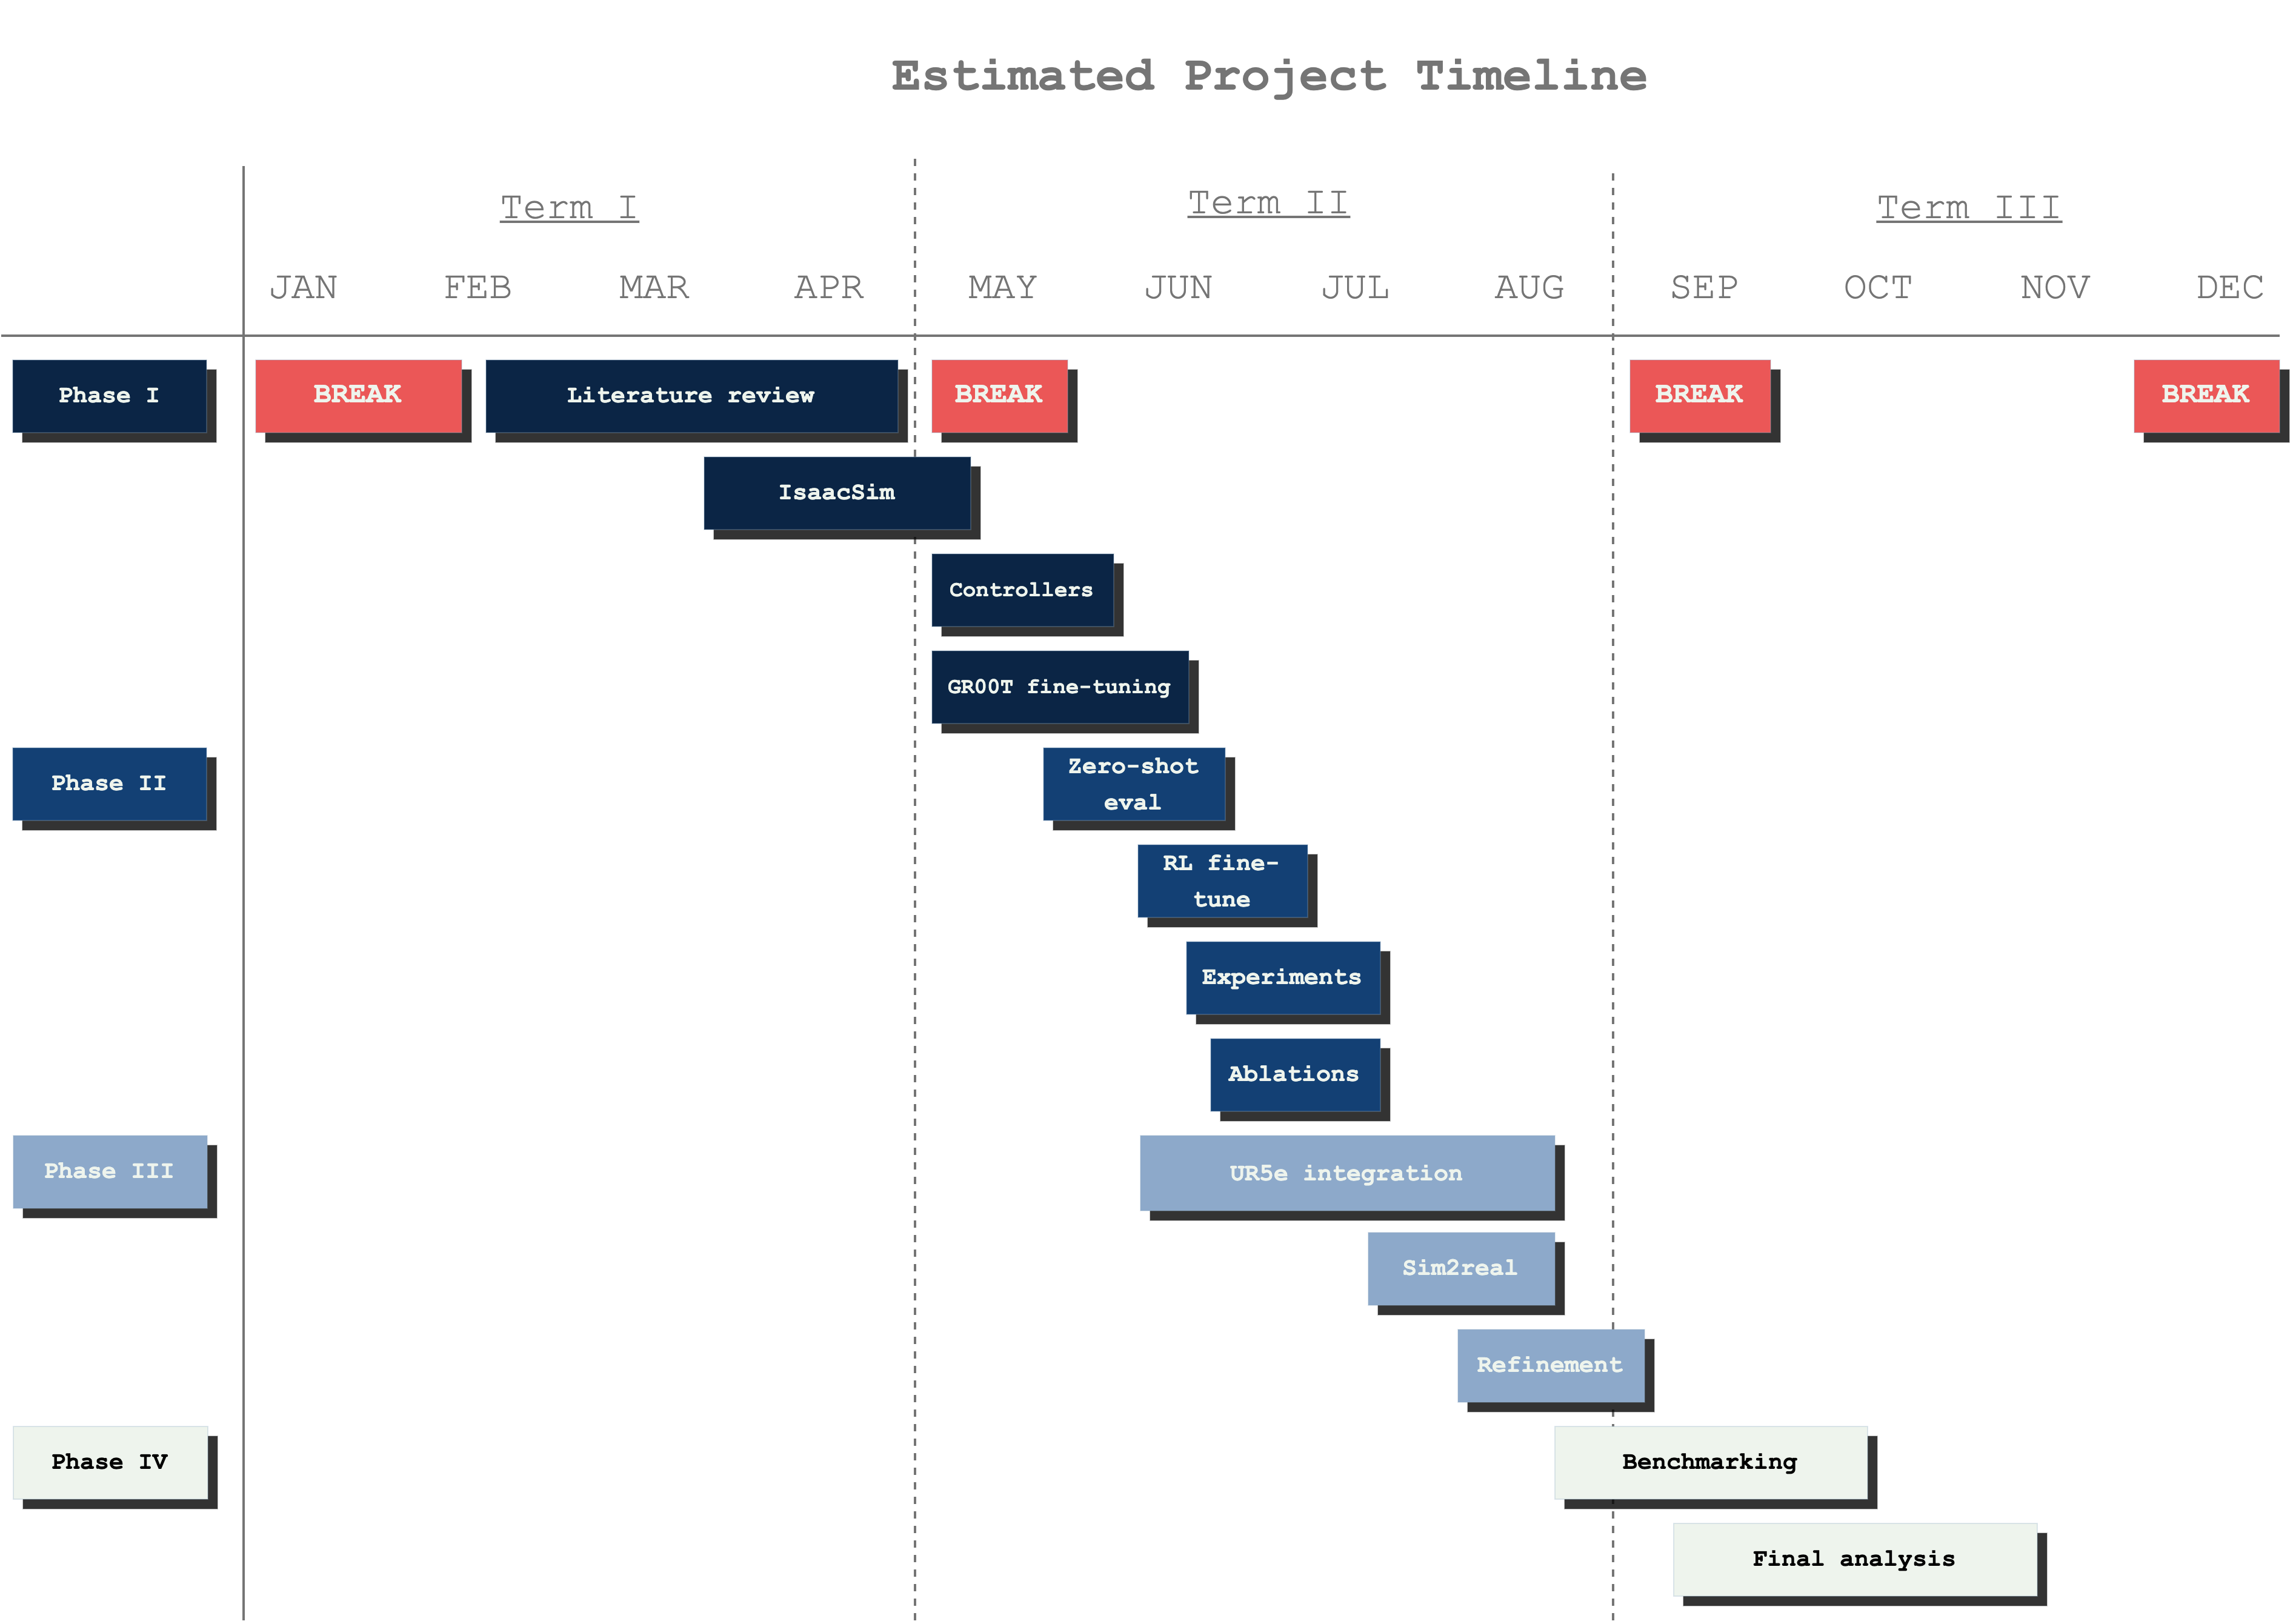
\includegraphics[width=\linewidth,height=0.75\textheight,keepaspectratio]{Figures/gantt.png}
%     \caption{Estimated project timeline broken down by academic term. The Gantt chart outlines four major phases of the project, beginning with simulation setup and literature review in Term 1, progressing through fine-tuning, evaluation, and integration in Term 2, and concluding with benchmarking and final analysis in Term 3. This timeline is a high-level guide and may be adjusted based on experimental findings and system performance.}
%     \label{fig:gantt}
% \end{figure}

\bigfigure[
    pos=H,
    opt={width=\linewidth,height=0.75\textheight,keepaspectratio},
    label={fig:gantt},
    shortcaption={Estimated project timeline by term, showing simulation setup, fine-tuning, evaluation, and final analysis phases.}
]
{gantt.png}
{Estimated project timeline broken down by academic term. The Gantt chart outlines four major phases of the project, beginning with simulation setup and literature review in Term 1, progressing through fine-tuning, evaluation, and integration in Term 2, and concluding with benchmarking and final analysis in Term 3. This timeline is a high-level guide and may be adjusted based on experimental findings and system performance.}

% \bigfigure[
%     pos=h,
%     opt={width=\linewidth},
%     \label{fig:gantt},
%     shortcaption={A short caption}
% ]
% {gantt.png}
% {Design process using a few \protect\acs{CFD} simulations (...) to be redone.}

\begin{widetablepages}
\begin{addmargin*}[0pt]{\fullmarginwidth}
\section{Full Discretized Task Progress Results}
\label{sec:appendix:results_monolith}

This appendix reports the per-trial \ac{DTP} scores $P_{\text{task}}$ for the frozen base policy, the three pure RL baselines (TD3, SAC, PPO), and their residual counterparts. Each method was evaluated on 20 physical rollouts per task under the 5--5--10 protocol.

The summary rows reproduce the values reported in \cref{tab:main_results_condensed}. Applying the metric definitions in \cref{sec:method:evaluation_metrics} to the printed trial rows gives different values for 60 of the 119 summary entries. For example, the 20 base-policy scores for \texttt{rubix-stack-v1} average 0.2500, while the reported mean is 0.2625. Reconciling these values requires the original rollout records.

\end{addmargin*}

\footnotesize
\begin{longtable}{@{\extracolsep{\fill}}l c *{7}{c} @{}}
    \caption[Full discretized task progress results]%
    {Full discretized task progress $P_{\text{task}}$ for all $7$ tasks and $20$ real-world rollouts per method. Columns report \ac{DTP} for the base policy, three pure RL baselines, and three residual RL adapters (\ac{TD3}, \ac{SAC}, \ac{PPO}) composed with the base policy. Trials are grouped into \ac{ID}, DP (dynamic perturbation), and \ac{OOD} conditions.}

    
    \label{tab:main_results} \\

    \toprule
    \multirow{2}{*}{\textbf{Block}} &
    \multirow{2}{*}{\textbf{Trial}} &
    % \multirow{2}{*}{\textbf{Base policy}} &
    \multirow{2}{*}{\shortstack[c]{\textbf{Base}\\\textbf{policy}}} &
    \multicolumn{3}{c}{\textbf{RL only}} &
    \multicolumn{3}{c}{\textbf{Residual}} \\
    \cmidrule(lr){4-6}\cmidrule(lr){7-9}
      &   &   & \textbf{TD3} & \textbf{SAC} & \textbf{PPO}
              & \textbf{TD3} & \textbf{SAC} & \textbf{PPO} \\
    \midrule
    \endfirsthead

    \multicolumn{9}{@{}l}{\textit{Table~\thetable\ (continued). Trials 1--5 are ID, 6--10 are DP, and 11--20 are OOD.}} \\
    \toprule
    \multirow{2}{*}{\textbf{Block}} &
    \multirow{2}{*}{\textbf{Trial}} &
    % \multirow{2}{*}{\textbf{Base policy}} &
    \multirow{2}{*}{\shortstack[c]{\textbf{Base}\\\textbf{policy}}} &
    \multicolumn{3}{c}{\textbf{RL only}} &
    \multicolumn{3}{c}{\textbf{Residual}} \\
    \cmidrule(lr){4-6}\cmidrule(lr){7-9}
      &   &   & \textbf{TD3} & \textbf{SAC} & \textbf{PPO}
              & \textbf{TD3} & \textbf{SAC} & \textbf{PPO} \\
    \midrule
    \endhead

    \midrule \multicolumn{9}{r@{}}{\textit{(continued on next page)}} \\
    \endfoot

    \bottomrule
    \endlastfoot

    %%%%%%%%%%%%%%%%%%%%%%%%%%%%%%%%%%%%%%%%%%%%%%%%%%%%%%%%%%%%%%
    % Task 1
    %%%%%%%%%%%%%%%%%%%%%%%%%%%%%%%%%%%%%%%%%%%%%%%%%%%%%%%%%%%%%%
    \multicolumn{9}{@{}l}{Task 1: \texttt{rubix-stack-v1}} \\*
    % --- In Distribution (1-5) ---
    \midrule
    \acs{ID}
      &  1 & 0.2500 & 0.2500 & 0.2500 & 0.2500 & 0.7500 & 0.5000 & 0.7500 \\
      &  2 & 0.5000 & 0.5000 & 0.5000 & 0.2500 & 0.7500 & 0.5000 & 0.7500 \\
      &  3 & 0.2500 & 0.2500 & 0.2500 & 0.2500 & 0.7500 & 0.5000 & 0.7500 \\
      &  4 & 0.5000 & 0.2500 & 0.2500 & 0.2500 & 0.7500 & 0.5000 & 0.7500 \\
      &  5 & 0.2500 & 0.2500 & 0.2500 & 0.2500 & 0.7500 & 0.5000 & 0.7500 \\
    \midrule
    % --- Dynamic Perturbation (6-10) ---
    DP
      &  6 & 0.5000 & 0.5000 & 0.5000 & 0.2500 & 0.7500 & 0.5000 & 0.7500 \\
      &  7 & 0.2500 & 0.2500 & 0.2500 & 0.2500 & 0.7500 & 0.5000 & 0.7500 \\
      &  8 & 0.5000 & 0.2500 & 0.2500 & 0.2500 & 0.7500 & 0.5000 & 0.7500 \\
      &  9 & 0.2500 & 0.2500 & 0.2500 & 0.2500 & 0.7500 & 0.5000 & 0.7500 \\
      & 10 & 0.5000 & 0.5000 & 0.5000 & 0.2500 & 0.7500 & 0.5000 & 0.7500 \\
    \midrule
    % --- OOD (11-20) ---
    \acs{OOD}
      & 11 & 0.2500 & 0.2500 & 0.2500 & 0.2500 & 0.7500 & 0.5000 & 0.7500 \\
      & 12 & 0.0000 & 0.0000 & 0.2500 & 0.0000 & 0.5000 & 0.2500 & 0.5000 \\
      & 13 & 0.2500 & 0.2500 & 0.5000 & 0.2500 & 0.7500 & 0.5000 & 0.7500 \\
      & 14 & 0.0000 & 0.0000 & 0.2500 & 0.0000 & 0.5000 & 0.2500 & 0.5000 \\
      & 15 & 0.2500 & 0.2500 & 0.0000 & 0.2500 & 0.7500 & 0.5000 & 0.7500 \\
      & 16 & 0.0000 & 0.0000 & 0.2500 & 0.0000 & 0.5000 & 0.2500 & 0.5000 \\
      & 17 & 0.2500 & 0.2500 & 0.2500 & 0.2500 & 0.7500 & 0.5000 & 0.7500 \\
      & 18 & 0.0000 & 0.0000 & 0.2500 & 0.0000 & 0.5000 & 0.2500 & 0.5000 \\
      & 19 & 0.2500 & 0.2500 & 0.5000 & 0.2500 & 0.7500 & 0.5000 & 0.7500 \\
      & 20 & 0.0000 & 0.0000 & 0.2500 & 0.0000 & 0.5000 & 0.2500 & 0.5000 \\
    \midrule
    \addlinespace
    \multicolumn{2}{r}{Mean progress $MP$}             &
        0.2625 & 0.2375 & 0.2750 & 0.2125 & 0.6750 & 0.4375 & 0.6750 \\
    \multicolumn{2}{r}{Generalization $J_{\text{gen}}$} &
        0.1250 & 0.1250 & 0.2500 & 0.1250 & 0.6000 & 0.3750 & 0.6000 \\
    \multicolumn{2}{r}{Transfer gap $\Delta_{\text{gen}}$} &
        \multicolumn{1}{c}{--} &  % Base
        \multicolumn{1}{c}{--} &  % RL TD3
        \multicolumn{1}{c}{--} &  % RL SAC
        \multicolumn{1}{c}{--} &  % RL PPO
        \multicolumn{1}{c}{0.4750} & % Res TD3
        \multicolumn{1}{c}{0.2500} & % Res SAC
        \multicolumn{1}{c}{0.4750}   % Res PPO
        \\
    \addlinespace
    \midrule

    %%%%%%%%%%%%%%%%%%%%%%%%%%%%%%%%%%%%%%%%%%%%%%%%%%%%%%%%%%%%%%
    % Task 2
    %%%%%%%%%%%%%%%%%%%%%%%%%%%%%%%%%%%%%%%%%%%%%%%%%%%%%%%%%%%%%%
    \multicolumn{9}{@{}l}{Task 2: \texttt{bus-table-easy-v1}} \\*
    % --- In Distribution (1-5) ---
    \midrule
    \acs{ID}
      &  1 & 0.2500 & 0.0000 & 0.0000 & 0.0000 & 0.2500 & 0.2500 & 0.2500 \\
      &  2 & 0.5000 & 0.2500 & 0.2500 & 0.2500 & 0.5000 & 0.5000 & 0.5000 \\
      &  3 & 0.2500 & 0.0000 & 0.5000 & 0.0000 & 0.2500 & 0.2500 & 0.2500 \\
      &  4 & 0.5000 & 0.2500 & 0.2500 & 0.2500 & 0.5000 & 0.5000 & 0.5000 \\
      &  5 & 0.2500 & 0.0000 & 0.0000 & 0.0000 & 0.2500 & 0.2500 & 0.2500 \\
    \midrule
    % --- Dynamic Perturbation (6-10) ---
    DP
      &  6 & 0.5000 & 0.2500 & 0.2500 & 0.2500 & 0.5000 & 0.5000 & 0.5000 \\
      &  7 & 0.2500 & 0.0000 & 0.5000 & 0.0000 & 0.2500 & 0.2500 & 0.2500 \\
      &  8 & 0.5000 & 0.2500 & 0.2500 & 0.2500 & 0.5000 & 0.5000 & 0.5000 \\
      &  9 & 0.2500 & 0.0000 & 0.0000 & 0.0000 & 0.2500 & 0.2500 & 0.2500 \\
      & 10 & 0.5000 & 0.2500 & 0.2500 & 0.2500 & 0.5000 & 0.5000 & 0.5000 \\
    \midrule
    % --- OOD (11-20) ---
    \acs{OOD}
      & 11 & 0.2500 & 0.2500 & 0.2500 & 0.2500 & 0.5000 & 0.5000 & 0.5000 \\
      & 12 & 0.7500 & 0.7500 & 0.7500 & 0.7500 & 1.0000 & 0.7500 & 1.0000 \\
      & 13 & 0.5000 & 0.5000 & 0.5000 & 0.5000 & 0.7500 & 0.7500 & 0.7500 \\
      & 14 & 0.7500 & 0.7500 & 1.0000 & 0.7500 & 1.0000 & 1.0000 & 1.0000 \\
      & 15 & 0.5000 & 0.5000 & 0.5000 & 0.5000 & 0.7500 & 0.7500 & 0.7500 \\
      & 16 & 0.7500 & 0.7500 & 0.7500 & 0.5000 & 1.0000 & 1.0000 & 1.0000 \\
      & 17 & 0.5000 & 0.5000 & 0.5000 & 0.5000 & 0.7500 & 0.7500 & 0.7500 \\
      & 18 & 0.7500 & 0.7500 & 0.7500 & 0.7500 & 1.0000 & 0.7500 & 1.0000 \\
      & 19 & 0.5000 & 0.5000 & 0.5000 & 0.5000 & 0.7500 & 0.7500 & 0.7500 \\
      & 20 & 0.7500 & 0.7500 & 1.0000 & 0.7500 & 1.0000 & 1.0000 & 1.0000 \\
    \midrule
    \addlinespace
    \multicolumn{2}{r}{Mean progress $MP$}             &
        0.5000 & 0.3625 & 0.4500 & 0.3375 & 0.6750 & 0.6000 & 0.6750 \\
    \multicolumn{2}{r}{Generalization $J_{\text{gen}}$} &
        0.6250 & 0.6250 & 0.6750 & 0.5750 & 0.8750 & 0.8000 & 0.8750 \\
    \multicolumn{2}{r}{Transfer gap $\Delta_{\text{gen}}$} &
        \multicolumn{1}{c}{--} &  % Base
        \multicolumn{1}{c}{--} &  % RL TD3
        \multicolumn{1}{c}{--} &  % RL SAC
        \multicolumn{1}{c}{--} &  % RL PPO
        \multicolumn{1}{c}{0.2500} & % Res TD3
        \multicolumn{1}{c}{0.1750} & % Res SAC
        \multicolumn{1}{c}{0.2500}   % Res PPO
        \\
    \addlinespace
    \midrule

    %%%%%%%%%%%%%%%%%%%%%%%%%%%%%%%%%%%%%%%%%%%%%%%%%%%%%%%%%%%%%%
    % Task 3
    %%%%%%%%%%%%%%%%%%%%%%%%%%%%%%%%%%%%%%%%%%%%%%%%%%%%%%%%%%%%%%
    \multicolumn{9}{@{}l}{Task 3: \texttt{bus-table-medium-v1}} \\*
    % --- In Distribution (1-5) ---
    \midrule
    \acs{ID}
      &  1 & 0.2500 & 0.0000 & 0.2500 & 0.0000 & 0.2500 & 0.2500 & 0.2500 \\
      &  2 & 0.5000 & 0.2500 & 0.2500 & 0.2500 & 0.5000 & 0.5000 & 0.5000 \\
      &  3 & 0.2500 & 0.0000 & 0.0000 & 0.0000 & 0.2500 & 0.2500 & 0.2500 \\
      &  4 & 0.5000 & 0.2500 & 0.2500 & 0.2500 & 0.5000 & 0.7500 & 0.5000 \\
      &  5 & 0.2500 & 0.0000 & 0.2500 & 0.0000 & 0.2500 & 0.2500 & 0.2500 \\
    \midrule
    % --- Dynamic Perturbation (6-10) ---
    DP
      &  6 & 0.5000 & 0.2500 & 0.2500 & 0.2500 & 0.5000 & 0.5000 & 0.5000 \\
      &  7 & 0.2500 & 0.0000 & 0.0000 & 0.0000 & 0.2500 & 0.2500 & 0.2500 \\
      &  8 & 0.5000 & 0.2500 & 0.2500 & 0.2500 & 0.5000 & 0.7500 & 0.5000 \\
      &  9 & 0.2500 & 0.0000 & 0.2500 & 0.0000 & 0.2500 & 0.2500 & 0.2500 \\
      & 10 & 0.5000 & 0.2500 & 0.2500 & 0.2500 & 0.5000 & 0.5000 & 0.5000 \\
    \midrule
    % --- OOD (11-20) ---
    \acs{OOD}
      & 11 & 0.2500 & 0.0000 & 0.0000 & 0.0000 & 0.5000 & 0.2500 & 0.5000 \\
      & 12 & 0.2500 & 0.2500 & 0.2500 & 0.2500 & 0.7500 & 0.7500 & 0.7500 \\
      & 13 & 0.0000 & 0.0000 & 0.2500 & 0.0000 & 0.5000 & 0.5000 & 0.5000 \\
      & 14 & 0.2500 & 0.2500 & 0.5000 & 0.2500 & 0.7500 & 0.7500 & 0.7500 \\
      & 15 & 0.0000 & 0.0000 & 0.2500 & 0.0000 & 0.5000 & 0.5000 & 0.5000 \\
      & 16 & 0.2500 & 0.2500 & 0.0000 & 0.0000 & 0.5000 & 0.5000 & 0.5000 \\
      & 17 & 0.0000 & 0.0000 & 0.2500 & 0.2500 & 0.5000 & 0.5000 & 0.5000 \\
      & 18 & 0.2500 & 0.2500 & 0.2500 & 0.2500 & 0.7500 & 0.7500 & 0.7500 \\
      & 19 & 0.0000 & 0.0000 & 0.2500 & 0.0000 & 0.5000 & 0.5000 & 0.5000 \\
      & 20 & 0.2500 & 0.2500 & 0.5000 & 0.2500 & 0.7500 & 0.7500 & 0.7500 \\
    \midrule
    \addlinespace
    \multicolumn{2}{r}{Mean progress $MP$}             &
        0.3125 & 0.1875 & 0.3125 & 0.1750 & 0.5500 & 0.5375 & 0.5250 \\
    \multicolumn{2}{r}{Generalization $J_{\text{gen}}$} &
        0.2500 & 0.1500 & 0.2750 & 0.1250 & 0.6000 & 0.6000 & 0.6000 \\
    \multicolumn{2}{r}{Transfer gap $\Delta_{\text{gen}}$} &
        \multicolumn{1}{c}{--} &  % Base
        \multicolumn{1}{c}{--} &  % RL TD3
        \multicolumn{1}{c}{--} &  % RL SAC
        \multicolumn{1}{c}{--} &  % RL PPO
        \multicolumn{1}{c}{0.3500} & % Res TD3
        \multicolumn{1}{c}{0.4500} & % Res SAC
        \multicolumn{1}{c}{0.3500}   % Res PPO
        \\
    \addlinespace
    \midrule

    %%%%%%%%%%%%%%%%%%%%%%%%%%%%%%%%%%%%%%%%%%%%%%%%%%%%%%%%%%%%%%
    % Task 4
    %%%%%%%%%%%%%%%%%%%%%%%%%%%%%%%%%%%%%%%%%%%%%%%%%%%%%%%%%%%%%%
    \multicolumn{9}{@{}l}{Task 4: \texttt{bus-table-hard-v1}} \\*
    % --- In Distribution (1-5) ---
    \midrule
    \acs{ID}
      &  1 & 0.0000 & 0.0000 & 0.0000 & 0.0000 & 0.2500 & 0.2500 & 0.2500 \\
      &  2 & 0.2500 & 0.2500 & 0.2500 & 0.0000 & 0.5000 & 0.5000 & 0.5000 \\
      &  3 & 0.0000 & 0.0000 & 0.0000 & 0.0000 & 0.2500 & 0.2500 & 0.2500 \\
      &  4 & 0.2500 & 0.0000 & 0.2500 & 0.0000 & 0.5000 & 0.5000 & 0.5000 \\
      &  5 & 0.0000 & 0.0000 & 0.0000 & 0.0000 & 0.2500 & 0.2500 & 0.2500 \\
    \midrule
    % --- Dynamic Perturbation (6-10) ---
    DP
      &  6 & 0.2500 & 0.2500 & 0.2500 & 0.0000 & 0.5000 & 0.5000 & 0.5000 \\
      &  7 & 0.0000 & 0.0000 & 0.0000 & 0.0000 & 0.2500 & 0.2500 & 0.2500 \\
      &  8 & 0.2500 & 0.0000 & 0.2500 & 0.0000 & 0.5000 & 0.5000 & 0.5000 \\
      &  9 & 0.0000 & 0.0000 & 0.0000 & 0.0000 & 0.2500 & 0.2500 & 0.2500 \\
      & 10 & 0.2500 & 0.2500 & 0.2500 & 0.0000 & 0.5000 & 0.5000 & 0.5000 \\
    \midrule
    % --- OOD (11-20) ---
    \acs{OOD}
      & 11 & 0.0000 & 0.0000 & 0.2500 & 0.0000 & 0.5000 & 0.5000 & 0.5000 \\
      & 12 & 0.0000 & 0.2500 & 0.0000 & 0.2500 & 0.5000 & 0.5000 & 0.5000 \\
      & 13 & 0.2500 & 0.0000 & 0.2500 & 0.0000 & 0.7500 & 0.7500 & 0.7500 \\
      & 14 & 0.0000 & 0.2500 & 0.0000 & 0.2500 & 0.5000 & 0.7500 & 0.5000 \\
      & 15 & 0.2500 & 0.0000 & 0.2500 & 0.0000 & 0.7500 & 0.7500 & 0.7500 \\
      & 16 & 0.0000 & 0.2500 & 0.0000 & 0.2500 & 0.5000 & 0.5000 & 0.5000 \\
      & 17 & 0.2500 & 0.0000 & 0.2500 & 0.0000 & 0.7500 & 0.7500 & 0.7500 \\
      & 18 & 0.0000 & 0.2500 & 0.0000 & 0.2500 & 0.5000 & 0.7500 & 0.5000 \\
      & 19 & 0.2500 & 0.0000 & 0.2500 & 0.0000 & 0.7500 & 0.7500 & 0.7500 \\
      & 20 & 0.0000 & 0.2500 & 0.0000 & 0.2500 & 0.5000 & 0.5000 & 0.5000 \\
    \midrule
    \addlinespace
    \multicolumn{2}{r}{Mean progress $MP$}             &
        0.2188 & 0.1562 & 0.2188 & 0.0625 & 0.5625 & 0.5312 & 0.5312 \\
    \multicolumn{2}{r}{Generalization $J_{\text{gen}}$} &
        0.1250 & 0.1250 & 0.2250 & 0.1250 & 0.6000 & 0.6250 & 0.6000 \\
    \multicolumn{2}{r}{Transfer gap $\Delta_{\text{gen}}$} &
        \multicolumn{1}{c}{--} &  % Base
        \multicolumn{1}{c}{--} &  % RL TD3
        \multicolumn{1}{c}{--} &  % RL SAC
        \multicolumn{1}{c}{--} &  % RL PPO
        \multicolumn{1}{c}{0.4750} & % Res TD3
        \multicolumn{1}{c}{0.5000} & % Res SAC
        \multicolumn{1}{c}{0.4750}   % Res PPO
        \\
    \addlinespace
    \midrule

    %%%%%%%%%%%%%%%%%%%%%%%%%%%%%%%%%%%%%%%%%%%%%%%%%%%%%%%%%%%%%%
    % Task 5
    %%%%%%%%%%%%%%%%%%%%%%%%%%%%%%%%%%%%%%%%%%%%%%%%%%%%%%%%%%%%%%
    \multicolumn{9}{@{}l}{Task 5: \texttt{close-bottle-lid-v1}} \\*
    % --- In Distribution (1-5) ---
    \midrule
    \acs{ID}
      &  1 & 0.7500 & 0.2500 & 0.2500 & 0.2500 & 0.5000 & 0.5000 & 0.7500 \\
      &  2 & 0.7500 & 0.2500 & 0.5000 & 0.2500 & 0.7500 & 0.7500 & 0.7500 \\
      &  3 & 0.5000 & 0.2500 & 0.2500 & 0.2500 & 0.5000 & 0.5000 & 0.7500 \\
      &  4 & 0.7500 & 0.2500 & 0.5000 & 0.2500 & 0.7500 & 0.7500 & 0.7500 \\
      &  5 & 0.7500 & 0.2500 & 0.2500 & 0.2500 & 0.5000 & 0.5000 & 0.7500 \\
    \midrule
    % --- Dynamic Perturbation (6-10) ---
    DP
      &  6 & 0.7500 & 0.2500 & 0.5000 & 0.2500 & 0.7500 & 0.7500 & 0.7500 \\
      &  7 & 0.5000 & 0.2500 & 0.2500 & 0.2500 & 0.5000 & 0.5000 & 0.7500 \\
      &  8 & 0.7500 & 0.2500 & 0.5000 & 0.2500 & 0.7500 & 0.7500 & 0.7500 \\
      &  9 & 0.7500 & 0.2500 & 0.2500 & 0.2500 & 0.5000 & 0.5000 & 0.7500 \\
      & 10 & 0.5000 & 0.2500 & 0.5000 & 0.2500 & 0.7500 & 0.7500 & 0.7500 \\
    \midrule
    % --- OOD (11-20) ---
    \acs{OOD}
      & 11 & 0.5000 & 0.2500 & 0.2500 & 0.2500 & 0.5000 & 0.5000 & 0.7500 \\
      & 12 & 0.5000 & 0.5000 & 0.5000 & 0.5000 & 0.7500 & 0.7500 & 0.7500 \\
      & 13 & 0.2500 & 0.2500 & 0.5000 & 0.2500 & 0.5000 & 0.7500 & 0.7500 \\
      & 14 & 0.5000 & 0.5000 & 0.5000 & 0.5000 & 0.7500 & 0.7500 & 0.7500 \\
      & 15 & 0.2500 & 0.2500 & 0.2500 & 0.2500 & 0.5000 & 0.5000 & 0.7500 \\
      & 16 & 0.5000 & 0.5000 & 0.5000 & 0.5000 & 0.7500 & 0.7500 & 0.7500 \\
      & 17 & 0.2500 & 0.2500 & 0.5000 & 0.2500 & 0.5000 & 0.7500 & 0.7500 \\
      & 18 & 0.5000 & 0.5000 & 0.5000 & 0.5000 & 0.7500 & 0.7500 & 0.7500 \\
      & 19 & 0.2500 & 0.2500 & 0.2500 & 0.2500 & 0.5000 & 0.5000 & 0.7500 \\
      & 20 & 0.5000 & 0.5000 & 0.5000 & 0.5000 & 0.7500 & 0.7500 & 0.7500 \\
    \midrule
    \addlinespace
    \multicolumn{2}{r}{Mean progress $MP$}             &
        0.5750 & 0.3125 & 0.4375 & 0.3125 & 0.6250 & 0.6500 & 0.7500 \\
    \multicolumn{2}{r}{Generalization $J_{\text{gen}}$} &
        0.4000 & 0.3750 & 0.4250 & 0.3750 & 0.6500 & 0.7000 & 0.7500 \\
    \multicolumn{2}{r}{Transfer gap $\Delta_{\text{gen}}$} &
        \multicolumn{1}{c}{--} &  % Base
        \multicolumn{1}{c}{--} &  % RL TD3
        \multicolumn{1}{c}{--} &  % RL SAC
        \multicolumn{1}{c}{--} &  % RL PPO
        \multicolumn{1}{c}{0.2500} & % Res TD3
        \multicolumn{1}{c}{0.3000} & % Res SAC
        \multicolumn{1}{c}{0.3500}   % Res PPO
        \\
    \addlinespace
    \midrule

    %%%%%%%%%%%%%%%%%%%%%%%%%%%%%%%%%%%%%%%%%%%%%%%%%%%%%%%%%%%%%%
    % Task 6
    %%%%%%%%%%%%%%%%%%%%%%%%%%%%%%%%%%%%%%%%%%%%%%%%%%%%%%%%%%%%%%
    \multicolumn{9}{@{}l}{Task 6: \texttt{erase-whiteboard-v1}} \\*
    % --- In Distribution (1-5) ---
    \midrule
    \acs{ID}
      &  1 & 1.0000 & 0.7500 & 0.7500 & 0.5000 & 1.0000 & 1.0000 & 1.0000 \\
      &  2 & 0.7500 & 0.7500 & 0.7500 & 0.7500 & 1.0000 & 1.0000 & 0.7500 \\
      &  3 & 1.0000 & 0.7500 & 1.0000 & 0.7500 & 1.0000 & 1.0000 & 1.0000 \\
      &  4 & 0.7500 & 0.7500 & 0.7500 & 0.7500 & 1.0000 & 1.0000 & 0.7500 \\
      &  5 & 1.0000 & 0.7500 & 1.0000 & 0.7500 & 1.0000 & 1.0000 & 1.0000 \\
    \midrule
    % --- Dynamic Perturbation (6-10) ---
    DP
      &  6 & 0.7500 & 0.7500 & 0.7500 & 0.7500 & 1.0000 & 1.0000 & 0.7500 \\
      &  7 & 1.0000 & 0.7500 & 1.0000 & 0.7500 & 1.0000 & 1.0000 & 1.0000 \\
      &  8 & 0.7500 & 0.7500 & 0.7500 & 0.7500 & 1.0000 & 1.0000 & 0.7500 \\
      &  9 & 1.0000 & 0.7500 & 1.0000 & 0.7500 & 1.0000 & 1.0000 & 1.0000 \\
      & 10 & 0.7500 & 0.7500 & 0.7500 & 0.7500 & 1.0000 & 1.0000 & 0.7500 \\
    \midrule
    % --- OOD (11-20) ---
    \acs{OOD}
      & 11 & 0.7500 & 0.5000 & 0.7500 & 0.5000 & 1.0000 & 1.0000 & 1.0000 \\
      & 12 & 0.7500 & 0.7500 & 0.7500 & 0.7500 & 0.7500 & 1.0000 & 0.7500 \\
      & 13 & 0.5000 & 0.5000 & 0.7500 & 0.5000 & 1.0000 & 1.0000 & 1.0000 \\
      & 14 & 0.7500 & 0.7500 & 1.0000 & 0.7500 & 1.0000 & 1.0000 & 1.0000 \\
      & 15 & 0.7500 & 0.5000 & 0.7500 & 0.5000 & 0.7500 & 1.0000 & 1.0000 \\
      & 16 & 0.7500 & 0.7500 & 0.7500 & 0.5000 & 1.0000 & 1.0000 & 1.0000 \\
      & 17 & 0.5000 & 0.5000 & 0.5000 & 0.5000 & 1.0000 & 1.0000 & 1.0000 \\
      & 18 & 0.7500 & 0.7500 & 0.7500 & 0.7500 & 1.0000 & 1.0000 & 0.7500 \\
      & 19 & 0.7500 & 0.5000 & 1.0000 & 0.5000 & 0.7500 & 1.0000 & 1.0000 \\
      & 20 & 0.7500 & 0.7500 & 0.7500 & 0.7500 & 1.0000 & 1.0000 & 1.0000 \\
    \midrule
    \addlinespace
    \multicolumn{2}{r}{Mean progress $MP$}             &
        0.8125 & 0.6250 & 0.7875 & 0.6000 & 0.9625 & 1.0000 & 0.9625 \\
    \multicolumn{2}{r}{Generalization $J_{\text{gen}}$} &
        0.7000 & 0.6250 & 0.7750 & 0.6000 & 0.9250 & 1.0000 & 0.9500 \\
    \multicolumn{2}{r}{Transfer gap $\Delta_{\text{gen}}$} &
        \multicolumn{1}{c}{--} &  % Base
        \multicolumn{1}{c}{--} &  % RL TD3
        \multicolumn{1}{c}{--} &  % RL SAC
        \multicolumn{1}{c}{--} &  % RL PPO
        \multicolumn{1}{c}{0.2250} & % Res TD3
        \multicolumn{1}{c}{0.3000} & % Res SAC
        \multicolumn{1}{c}{0.2500}   % Res PPO
        \\
    \addlinespace
    \midrule

    %%%%%%%%%%%%%%%%%%%%%%%%%%%%%%%%%%%%%%%%%%%%%%%%%%%%%%%%%%%%%%
    % Task 7
    %%%%%%%%%%%%%%%%%%%%%%%%%%%%%%%%%%%%%%%%%%%%%%%%%%%%%%%%%%%%%%
    \multicolumn{9}{@{}l}{Task 7: \texttt{close-french-press-v1}} \\*
    % --- In Distribution (1-5) ---
    \midrule
    \acs{ID}
      &  1 & 0.7500 & 0.0000 & 0.2500 & 0.0000 & 0.5000 & 0.7500 & 0.5000 \\
      &  2 & 0.5000 & 0.2500 & 0.0000 & 0.2500 & 0.7500 & 0.7500 & 0.7500 \\
      &  3 & 0.7500 & 0.0000 & 0.2500 & 0.0000 & 0.5000 & 0.7500 & 0.5000 \\
      &  4 & 0.5000 & 0.2500 & 0.5000 & 0.2500 & 0.7500 & 1.0000 & 0.7500 \\
      &  5 & 0.7500 & 0.0000 & 0.0000 & 0.0000 & 0.7500 & 0.7500 & 0.7500 \\
    \midrule
    % --- Dynamic Perturbation (6-10) ---
    DP
      &  6 & 0.5000 & 0.2500 & 0.2500 & 0.2500 & 0.5000 & 0.7500 & 0.5000 \\
      &  7 & 0.7500 & 0.0000 & 0.2500 & 0.0000 & 0.7500 & 0.7500 & 0.7500 \\
      &  8 & 0.5000 & 0.2500 & 0.0000 & 0.2500 & 0.5000 & 0.7500 & 0.5000 \\
      &  9 & 0.7500 & 0.0000 & 0.5000 & 0.0000 & 0.7500 & 1.0000 & 0.7500 \\
      & 10 & 0.5000 & 0.2500 & 0.2500 & 0.2500 & 0.7500 & 0.7500 & 0.7500 \\
    \midrule
    % --- OOD (11-20) ---
    \acs{OOD}
      & 11 & 0.2500 & 0.0000 & 0.0000 & 0.0000 & 0.5000 & 0.7500 & 0.5000 \\
      & 12 & 0.0000 & 0.2500 & 0.2500 & 0.2500 & 0.7500 & 0.7500 & 0.7500 \\
      & 13 & 0.2500 & 0.0000 & 0.2500 & 0.0000 & 0.5000 & 0.5000 & 0.5000 \\
      & 14 & 0.0000 & 0.2500 & 0.0000 & 0.2500 & 0.5000 & 0.7500 & 0.5000 \\
      & 15 & 0.2500 & 0.0000 & 0.5000 & 0.2500 & 0.7500 & 0.7500 & 0.7500 \\
      & 16 & 0.0000 & 0.2500 & 0.2500 & 0.0000 & 0.5000 & 0.5000 & 0.5000 \\
      & 17 & 0.2500 & 0.0000 & 0.0000 & 0.2500 & 0.5000 & 0.7500 & 0.5000 \\
      & 18 & 0.0000 & 0.2500 & 0.2500 & 0.0000 & 0.7500 & 0.7500 & 0.7500 \\
      & 19 & 0.2500 & 0.0000 & 0.2500 & 0.2500 & 0.5000 & 0.5000 & 0.5000 \\
      & 20 & 0.0000 & 0.2500 & 0.0000 & 0.0000 & 0.7500 & 0.7500 & 0.7500 \\
    \midrule
    \addlinespace
    \multicolumn{2}{r}{Mean progress $MP$}             &
        0.3750 & 0.1250 & 0.2000 & 0.1250 & 0.6250 & 0.7375 & 0.6250 \\
    \multicolumn{2}{r}{Generalization $J_{\text{gen}}$} &
        0.1250 & 0.1250 & 0.1750 & 0.1250 & 0.6000 & 0.6750 & 0.6000 \\
    \multicolumn{2}{r}{Transfer gap $\Delta_{\text{gen}}$} &
        \multicolumn{1}{c}{--} &  % Base
        \multicolumn{1}{c}{--} &  % RL TD3
        \multicolumn{1}{c}{--} &  % RL SAC
        \multicolumn{1}{c}{--} &  % RL PPO
        \multicolumn{1}{c}{0.4750} & % Res TD3
        \multicolumn{1}{c}{0.5500} & % Res SAC
        \multicolumn{1}{c}{0.4750}   % Res PPO
        \\
    \addlinespace

    % \midrule

    % Repeat same pattern for Tasks 3–7
\end{longtable}
\end{widetablepages}

\section{SO-101 Bill of Materials}
\label{sec:bom}

The bill of materials in \cref{tab:so101_bom} provides a consolidated overview of all hardware components required to assemble the two-arm SO-101 setup, including servos, motor control boards, cabling, power supplies, mounting hardware, and tools.

\begin{table}[H]
  \myfloatalign
  \scriptsize
  \caption{Bill of materials for the SO-101 leader and follower robotic arms (two-arm setup).}
  \label{tab:so101_bom}
  \begin{tabularx}{\textwidth}{X c}
    \toprule
    \textbf{Part} & \textbf{Qty} \\
    \midrule
    STS3215 Servo 7.4V, 1/345 gear (C001) & 7 \\
    STS3215 Servo 7.4V, 1/191 gear (C044) & 2 \\
    STS3215 Servo 7.4V, 1/147 gear (C046) & 3 \\
    Motor control board & 2 \\
    USB-C cable (pack of 2) & 1 \\
    Power supply & 2 \\
    Table clamp (pack of 4) & 1 \\
    Screwdriver set & 1 \\
    \bottomrule
  \end{tabularx}
\end{table}

\newpage
\pagestyle{empty}

\hfill

\vfill

\pdfbookmark[-1]{Colophon}{colophon}
\section*{Colophon}
This document was typeset using the typographical look-and-feel \texttt{classicthesis} developed by Andr\'e Miede. 
The style was inspired by Robert Bringhurst's seminal book on typography ``\emph{The Elements of Typographic Style}''. 
\texttt{classicthesis} is available for both \LaTeX\ and \mLyX: 
\begin{center}
\url{https://bitbucket.org/amiede/classicthesis/}
\end{center}

\begin{spacedparagraphs}
\doclicenseImage

\myLicenseNotice{} (\doclicenseName).

You may copy and share this material for noncommercial purposes if you credit
the authors and link to the license. Commercial use and distribution of
adaptations require separate permission, subject to applicable copyright
exceptions and limitations. The license terms are available at
\expandafter\url\expandafter{\doclicenseURL}.
\end{spacedparagraphs}


%********************************************************************
% Other Stuff in the Back
%*******************************************************

% ********************************************************************
% Game Over: Restore, Restart, or Quit?
%*******************************************************

\end{document}
% ********************************************************************
